%% Run LaTeX on this file several times to get Table of Contents,
%% cross-references, and citations.

\documentclass[11pt]{book}
\usepackage{gvv-book}
\usepackage{gvv}
%\usepackage{Wiley-AuthoringTemplate}
\usepackage[sectionbib,authoryear]{natbib}% for name-date citation comment the below line
%\usepackage[sectionbib,numbers]{natbib}% for numbered citation comment the above line

%%********************************************************************%%
%%       How many levels of section head would you like numbered?     %%
%% 0= no section numbers, 1= section, 2= section, 3= subsection %%
\setcounter{secnumdepth}{3}
%%********************************************************************%%
%%**********************************************************************%%
%%     How many levels of section head would you like to appear in the  %%
%%				Table of Contents?			%%
%% 0= chapter, 1= section, 2= section, 3= subsection titles.	%%
\setcounter{tocdepth}{2}
%%**********************************************************************%%

%\includeonly{ch01}
\makeindex

\begin{document}

\frontmatter
%%%%%%%%%%%%%%%%%%%%%%%%%%%%%%%%%%%%%%%%%%%%%%%%%%%%%%%%%%%%%%%%
%% Title Pages
%% Wiley will provide title and copyright page, but you can make
%% your own titlepages if you'd like anyway
%% Setting up title pages, type in the appropriate names here:

\booktitle{Geometry}

\subtitle{Through Algebra}

\AuAff{G. V. V. Sharma}


%% \\ will start a new line.
%% You may add \affil{} for affiliation, ie,
%\authors{Robert M. Groves\\
%\affil{Universitat de les Illes Balears}
%Floyd J. Fowler, Jr.\\
%\affil{University of New Mexico}
%}

%% Print Half Title and Title Page:
%\halftitlepage
\titlepage

%%%%%%%%%%%%%%%%%%%%%%%%%%%%%%%%%%%%%%%%%%%%%%%%%%%%%%%%%%%%%%%%
%% Copyright Page

\begin{copyrightpage}{2022}
%Title, etc
\end{copyrightpage}

% Note, you must use \ to start indented lines, ie,
% 
% \begin{copyrightpage}{2004}
% Survey Methodology / Robert M. Groves . . . [et al.].
% \       p. cm.---(Wiley series in survey methodology)
% \    ``Wiley-Interscience."
% \    Includes bibliographical references and index.
% \    ISBN 0-471-48348-6 (pbk.)
% \    1. Surveys---Methodology.  2. Social 
% \  sciences---Research---Statistical methods.  I. Groves, Robert M.  II. %
% Series.\\

% HA31.2.S873 2004
% 001.4'33---dc22                                             2004044064
% \end{copyrightpage}

%%%%%%%%%%%%%%%%%%%%%%%%%%%%%%%%%%%%%%%%%%%%%%%%%%%%%%%%%%%%%%%%
%% Only Dedication (optional) 

%\dedication{To my parents}

\tableofcontents

%\listoffigures %optional
%\listoftables  %optional

%% or Contributor Page for edited books
%% before \tableofcontents

%%%%%%%%%%%%%%%%%%%%%%%%%%%%%%%%%%%%%%%%%%%%%%%%%%%%%%%%%%%%%%%%
%  Contributors Page for Edited Book
%%%%%%%%%%%%%%%%%%%%%%%%%%%%%%%%%%%%%%%%%%%%%%%%%%%%%%%%%%%%%%%%

% If your book has chapters written by different authors,
% you'll need a Contributors page.

% Use \begin{contributors}...\end{contributors} and
% then enter each author with the \name{} command, followed
% by the affiliation information.

% \begin{contributors}
% \name{Masayki Abe,} Fujitsu Laboratories Ltd., Fujitsu Limited, Atsugi, Japan
%
% \name{L. A. Akers,} Center for Solid State Electronics Research, Arizona State University, Tempe, Arizona
%
% \name{G. H. Bernstein,} Department of Electrical and Computer Engineering, University of Notre Dame, Notre Dame, South Bend, Indiana; formerly of
% Center for Solid State Electronics Research, Arizona
% State University, Tempe, Arizona 
% \end{contributors}

%%%%%%%%%%%%%%%%%%%%%%%%%%%%%%%%%%%%%%%%%%%%%%%%%%%%%%%%%%%%%%%%
% Optional Foreword:

%\begin{foreword}
%\lipsum[1-2]
%\end{foreword}

%%%%%%%%%%%%%%%%%%%%%%%%%%%%%%%%%%%%%%%%%%%%%%%%%%%%%%%%%%%%%%%%
% Optional Preface:

%\begin{preface}
%\lipsum[1-1]
%\prefaceauthor{}
%\where{place\\
% date}
%\end{preface}

% ie,
% \begin{preface}
% This is an example preface.
% \prefaceauthor{R. K. Watts}
% \where{Durham, North Carolina\\
% September, 2004}

%%%%%%%%%%%%%%%%%%%%%%%%%%%%%%%%%%%%%%%%%%%%%%%%%%%%%%%%%%%%%%%%
% Optional Acknowledgments:

%\acknowledgments
%\lipsum[1-2]
%\authorinitials{I. R. S.}  

%%%%%%%%%%%%%%%%%%%%%%%%%%%%%%%%
%% Glossary Type of Environment:

% \begin{glossary}
% \term{<term>}{<description>}
% \end{glossary}

%%%%%%%%%%%%%%%%%%%%%%%%%%%%%%%%
%\begin{acronyms}
%\acro{ASTA}{Arrivals See Time Averages}
%\acro{BHCA}{Busy Hour Call Attempts}
%\acro{BR}{Bandwidth Reservation}
%\acro{b.u.}{bandwidth unit(s)}
%\acro{CAC}{Call / Connection Admission Control}
%\acro{CBP}{Call Blocking Probability(-ies)}
%\acro{CCS}{Centum Call Seconds}
%\acro{CDTM}{Connection Dependent Threshold Model}
%\acro{CS}{Complete Sharing}
%\acro{DiffServ}{Differentiated Services}
%\acro{EMLM}{Erlang Multirate Loss Model}
%\acro{erl}{The Erlang unit of traffic-load}
%\acro{FIFO}{First in - First out}
%\acro{GB}{Global balance}
%\acro{GoS}{Grade of Service}
%\acro{ICT}{Information and Communication Technology}
%\acro{IntServ}{Integrated Services}
%\acro{IP}{Internet Protocol}
%\acro{ITU-T}{International Telecommunication Unit -- Standardization sector}
%\acro{LB}{Local balance}
%\acro{LHS}{Left hand side}
%\acro{LIFO}{Last in - First out}
%\acro{MMPP}{Markov Modulated Poisson Process}
%\acro{MPLS}{Multiple Protocol Labeling Switching}
%\acro{MRM}{Multi-Retry Model}
%\acro{MTM}{Multi-Threshold Model}
%\acro{PASTA}{Poisson Arrivals See Time Averages}
%\acro{PDF}{Probability Distribution Function}
%\acro{pdf}{probability density function}
%\acro{PFS}{Product Form Solution}
%\acro{QoS}{Quality of Service}
%\acro{r.v.}{random variable(s)}
%\acro{RED}{random early detection}
%\acro{RHS}{Right hand side}
%\acro{RLA}{Reduced Load Approximation}
%\acro{SIRO}{service in random order}
%\acro{SRM}{Single-Retry Model}
%\acro{STM}{Single-Threshold Model}
%\acro{TCP}{Transport Control Protocol}
%\acro{TH}{Threshold(s)}
%\acro{UDP}{User Datagram Protocol}
%\end{acronyms}

\setcounter{page}{1}

\begin{introduction}
This book shows how to solve problems in geometry using trigonometry and coordinate geometry. 

\end{introduction}

\mainmatter

\chapter{Triangle}
Consider a triangle with vertices
		\begin{align}
			\label{eq:tri-pts}
			\vec{A} = \myvec{1 \\ -1},\,
			\vec{B} = \myvec{-4 \\ 6},\,
			\vec{C} = \myvec{-3 \\ -5}
		\end{align}
\section{Vectors}
%\renewcommand{\theequation}{\theenumi}
%\begin{enumerate}[label=\arabic*.,ref=\theenumi]
\begin{enumerate}[label=\thesection.\arabic*.,ref=\thesection.\theenumi]
\numberwithin{equation}{enumi}
\item The direction vector of $AB$ is defined as
		\begin{align}
			\vec{B}-
			\vec{A}
		\end{align}
Find the direction vectors of $AB, BC$ and $CA$.
\\
	\iffalse
\let\negmedspace\undefined
\let\negthickspace\undefined
\documentclass[journal,12pt,twocolumn]{IEEEtran}
\usepackage{cite}
\usepackage{amsmath,amssymb,amsfonts,amsthm}
\usepackage{algorithmic}
\usepackage{graphicx}
\usepackage{textcomp}
\usepackage{xcolor}
\usepackage{txfonts}
\usepackage{listings}
\usepackage{enumitem}
\usepackage{mathtools}
\usepackage{gensymb}
\usepackage[breaklinks=true]{hyperref}
\usepackage{tkz-euclide} % loads  TikZ and tkz-base
\usepackage{listings}
\usepackage{gvv}
%
%\usepackage{setspace}
%\usepackage{gensymb}
%\doublespacing
%\singlespacing

%\usepackage{graphicx}
%\usepackage{amssymb}
%\usepackage{relsize}
%\usepackage[cmex10]{amsmath}
%\usepackage{amsthm}
%\interdisplaylinepenalty=2500
%\savesymbol{iint}
%\usepackage{txfonts}
%\restoresymbol{TXF}{iint}
%\usepackage{wasysym}
%\usepackage{amsthm}
%\usepackage{iithtlc}
%\usepackage{mathrsfs}
%\usepackage{txfonts}
%\usepackage{stfloats}
%\usepackage{bm}
%\usepackage{cite}
%\usepackage{cases}
%\usepackage{subfig}
%\usepackage{xtab}
%\usepackage{longtable}
%\usepackage{multirow}
%\usepackage{algorithm}
%\usepackage{algpseudocode}
%\usepackage{enumitem}
%\usepackage{mathtools}
%\usepackage{tikz}
%\usepackage{circuitikz}
%\usepackage{verbatim}
%\usepackage{tfrupee}
%\usepackage{stmaryrd}
%\usetkzobj{all}
%    \usepackage{color}                                            %%
%    \usepackage{array}                                            %%
%    \usepackage{longtable}                                        %%
%    \usepackage{calc}                                             %%
%    \usepackage{multirow}                                         %%
%    \usepackage{hhline}                                           %%
%    \usepackage{ifthen}                                           %%
  %optionally (for landscape tables embedded in another document): %%
%    \usepackage{lscape}     
%\usepackage{multicol}
%\usepackage{chngcntr}
%\usepackage{enumerate}

%\usepackage{wasysym}
%\documentclass[conference]{IEEEtran}
%\IEEEoverridecommandlockouts
% The preceding line is only needed to identify funding in the first footnote. If that is unneeded, please comment it out.

\newtheorem{theorem}{Theorem}[section]
\newtheorem{problem}{Problem}
\newtheorem{proposition}{Proposition}[section]
\newtheorem{lemma}{Lemma}[section]
\newtheorem{corollary}[theorem]{Corollary}
\newtheorem{example}{Example}[section]
\newtheorem{definition}[problem]{Definition}
%\newtheorem{thm}{Theorem}[section] 
%\newtheorem{defn}[thm]{Definition}
%\newtheorem{algorithm}{Algorithm}[section]
%\newtheorem{cor}{Corollary}
\newcommand{\BEQA}{\begin{eqnarray}}
\newcommand{\EEQA}{\end{eqnarray}}
\newcommand{\define}{\stackrel{\triangle}{=}}
\theoremstyle{remark}
\newtheorem{rem}{Remark}

%\bibliographystyle{ieeetr}
\begin{document}
%

\bibliographystyle{IEEEtran}


\vspace{3cm}

\title{
    Solution to problem number 1.1.1
}
\author{ Aditya Vikram Singh - EE22BTECH11001}
%\title{
%	\logo{Matrix Analysis through Octave}{\begin{center}\includegraphics[scale=.24]{tlc}\end{center}}{}{HAMDSP}
%}


% paper title
% can use linebreaks \\ within to get better formatting as desired
%\title{Matrix Analysis through Octave}
%
%
% author names and IEEE memberships
% note positions of commas and nonbreaking spaces ( ~ ) LaTeX will not break
% a structure at a ~ so this keeps an author's name from being broken across
% two lines.
% use \thanks{} to gain access to the first footnote area
% a separate \thanks must be used for each paragraph as LaTeX2e's \thanks
% was not built to handle multiple paragraphs
%

%\author{<-this % stops a space
%\thanks{}}
%}
% note the % following the last \IEEEmembership and also \thanks - 
% these prevent an unwanted space from occurring between the last author name
% and the end of the author line. i.e., if you had this:
% 
% \author{....lastname \thanks{...} \thanks{...} }
%                     ^------------^------------^----Do not want these spaces!
%
% a space would be appended to the last name and could cause every name on that
% line to be shifted left slightly. This is one of those "LaTeX things". For
% instance, "\textbf{A} \textbf{B}" will typeset as "A B" not "AB". To get
% "AB" then you have to do: "\textbf{A}\textbf{B}"
% \thanks is no different in this regard, so shield the last } of each \thanks
% that ends a line with a % and do not let a space in before the next \thanks.
% Spaces after \IEEEmembership other than the last one are OK (and needed) as
% you are supposed to have spaces between the names. For what it is worth,
% this is a minor point as most people would not even notice if the said evil
% space somehow managed to creep in.



% The paper headers
%\markboth{Journal of \LaTeX\ Class Files,~Vol.~6, No.~1, January~2007}%
%{Shell \MakeLowercase{\textit{et al.}}: Bare Demo of IEEEtran.cls for Journals}
% The only time the second header will appear is for the odd numbered pages
% after the title page when using the twoside option.
% 
% *** Note that you probably will NOT want to include the author's ***
% *** name in the headers of peer review papers.                   ***
% You can use \ifCLASSOPTIONpeerreview for conditional compilation here if
% you desire.




% If you want to put a publisher's ID mark on the page you can do it like
% this:
%\IEEEpubid{0000--0000/00\$00.00~\copyright~2007 IEEE}
% Remember, if you use this you must call \IEEEpubidadjcol in the second
% column for its text to clear the IEEEpubid mark.



% make the title area
\maketitle

\newpage

%\tableofcontents

\bigskip

\renewcommand{\thefigure}{\theenumi}
\renewcommand{\thetable}{\theenumi}
%\renewcommand{\theequation}{\theenumi}

%\begin{abstract}
%%\boldmath
%In this letter, an algorithm for evaluating the exact analytical bit error rate  (BER)  for the piecewise linear (PL) combiner for  multiple relays is presented. Previous results were available only for upto three relays. The algorithm is unique in the sense that  the actual mathematical expressions, that are prohibitively large, need not be explicitly obtained. The diversity gain due to multiple relays is shown through plots of the analytical BER, well supported by simulations. 
%
%\end{abstract}
% IEEEtran.cls defaults to using nonbold math in the Abstract.
% This preserves the distinction between vectors and scalars. However,
% if the journal you are submitting to favors bold math in the abstract,
% then you can use LaTeX's standard command \boldmath at the very start
% of the abstract to achieve this. Many IEEE journals frown on math
% in the abstract anyway.

% Note that keywords are not normally used for peerreview papers.
%\begin{IEEEkeywords}
%Cooperative diversity, decode and forward, piecewise linear
%\end{IEEEkeywords}



% For peer review papers, you can put extra information on the cover
% page as needed:
% \ifCLASSOPTIONpeerreview
% \begin{center} \bfseries EDICS Category: 3-BBND \end{center}
% \fi
%
% For peerreview papers, this IEEEtran command inserts a page break and
% creates the second title. It will be ignored for other modes.
%\IEEEpeerreviewmaketitle
Consider a triangle with vertices
\begin{align} 
 \vec{A} &= \myvec{ 1\\ -1 } \\ \vec{B} &= \myvec{ -4\\ 6 }
  \\\vec{C} &= \myvec{ -3\\ -5}
 \end{align}
\textbf{Question}1.1.1\\  The Direction Vector of $AB$ is defined as 
  %The given coordinates are \\
\begin{align} 
\vec{B} - \vec{A}
\end{align}
Find the Direction Vectors of $AB$,$BC$,$CA$.\\
\fi
\solution %\begin{align} 
 %\vec{A} &= \myvec{ 1\\ -1 } \\ \vec{B} &= \myvec{ -4\\ 6 }
  %\\\vec{C} &= \myvec{ -3\\ -5}
 %\end{align}


\begin{enumerate} 
\item  The Direction vector of $AB$ is \begin{align} &= \vec{B} - \vec{A} \\
 &= \myvec{ -4 - (1)\\ 6 - (-1) } \\&= \myvec{ -5\\ 7 }
 \end{align}
\item The Direction vector of $BC$ \begin{align}&= \vec{C} - \vec{B}\\
 &= \myvec{ -3 - (-4)\\ -5 - (6) } \\&= \myvec{1\\ -11 }
  \end{align}
  \item  The Direction vector of $CA$  \begin{align} &= \vec{A} - \vec{C} \\ 
 &= \myvec{ 1 - (-3)\\ -1 - (-5) } \\&= \myvec{ 4\\ 4 }
  \end{align}
 \end{enumerate}


	\item The length of side $BC$ is 
		\begin{align}
			\norm{\vec{B}-\vec{A}} \triangleq \sqrt{\brak{\vec{B}-\vec{A}}^{\top}{\vec{B}-\vec{A}}}
		\end{align}
		where
		\begin{align}
			\vec{A}^{\top}\triangleq\myvec{1 & -1}
		\end{align}
\item   Points $\vec{A}, \vec{B}, \vec{C}$ are defined to be collinear if 
		\begin{align}
			\rank{\myvec{1 & 1 & 1 \\ \vec{A}& \vec{B}&\vec{C}}} = 2
		\end{align}
Are the given points in
			\eqref{eq:tri-pts}
collinear?
\item The parameteric form of the equation  of $AB$ is 
		\begin{align}
			\vec{x}=\vec{A}+k\vec{m}
		\end{align}
		where
		\begin{align}
\vec{m}=\vec{B}-\vec{A}
		\end{align}
is the direction vector of $AB$.
Find the parameteric equations of $AB, BC$ and $CA$.
\\
		\iffalse
\let\negmedspace\undefined
\let\negthickspace\undefined
\documentclass[journal,12pt,twocolumn]{IEEEtran}
\usepackage{cite}
\usepackage{amsmath,amssymb,amsfonts,amsthm}
\usepackage{algorithmic}
\usepackage{graphicx}
\usepackage{textcomp}
\usepackage{xcolor}
\usepackage{txfonts}
\usepackage{listings}
\usepackage{enumitem}
\usepackage{mathtools}
\usepackage{gensymb}
\usepackage[breaklinks=true]{hyperref}
\usepackage{tkz-euclide} % loads  TikZ and tkz-base
\usepackage{listings}
%\usepackage{gvv}

\newtheorem{theorem}{Theorem}[section]
\newtheorem{problem}{Problem}
\newtheorem{proposition}{Proposition}[section]
\newtheorem{lemma}{Lemma}[section]
\newtheorem{corollary}[theorem]{Corollary}
\newtheorem{example}{Example}[section]
\newtheorem{definition}[problem]{Definition}
\newcommand{\BEQA}{\begin{eqnarray}}
\newcommand{\EEQA}{\end{eqnarray}}
\newcommand{\define}{\stackrel{\triangle}{=}}
\theoremstyle{remark}
\newtheorem{rem}{Remark}

\begin{document}
\bibliographystyle{IEEEtran}
\vspace{3cm}
\title{
%	\logo{
Assignment
%	}
}
\author{ Antalene (EE22BTECH11008)}
\maketitle
\newpage
\bigskip
\renewcommand{\thefigure}{\theenumi}
\renewcommand{\thetable}{\theenumi}

\providecommand{\pr}[1]{\ensuremath{\Pr\left(#1\right)}}
\providecommand{\prt}[2]{\ensuremath{p_{#1}^{\left(#2\right)} }}        % own macro for this question
\providecommand{\qfunc}[1]{\ensuremath{Q\left(#1\right)}}
\providecommand{\sbrak}[1]{\ensuremath{{}\left[#1\right]}}
\providecommand{\lsbrak}[1]{\ensuremath{{}\left[#1\right.}}
\providecommand{\rsbrak}[1]{\ensuremath{{}\left.#1\right]}}
\providecommand{\brak}[1]{\ensuremath{\left(#1\right)}}
\providecommand{\lbrak}[1]{\ensuremath{\left(#1\right.}}
\providecommand{\rbrak}[1]{\ensuremath{\left.#1\right)}}
\providecommand{\cbrak}[1]{\ensuremath{\left\{#1\right\}}}
\providecommand{\lcbrak}[1]{\ensuremath{\left\{#1\right.}}
\providecommand{\rcbrak}[1]{\ensuremath{\left.#1\right\}}}
\newcommand{\sgn}{\mathop{\mathrm{sgn}}}
\providecommand{\abs}[1]{\left\vert#1\right\vert}
\providecommand{\res}[1]{\Res\displaylimits_{#1}} 
\providecommand{\norm}[1]{\left\lVert#1\right\rVert}
%\providecommand{\norm}[1]{\lVert#1\rVert}
\providecommand{\mtx}[1]{\mathbf{#1}}
\providecommand{\mean}[1]{E\left[ #1 \right]}
\providecommand{\cond}[2]{#1\middle|#2}
\providecommand{\fourier}{\overset{\mathcal{F}}{ \rightleftharpoons}}
\newenvironment{amatrix}[1]{%
  \left(\begin{array}{@{}*{#1}{c}|c@{}}
}{%
  \end{array}\right)
}
%\providecommand{\hilbert}{\overset{\mathcal{H}}{ \rightleftharpoons}}
%\providecommand{\system}{\overset{\mathcal{H}}{ \longleftrightarrow}}
	%\newcommand{\solution}[2]{\textbf{Solution:}{#1}}
\newcommand{\solution}{\noindent \textbf{Solution: }}
\newcommand{\cosec}{\,\text{cosec}\,}
\providecommand{\dec}[2]{\ensuremath{\overset{#1}{\underset{#2}{\gtrless}}}}
\newcommand{\myvec}[1]{\ensuremath{\begin{pmatrix}#1\end{pmatrix}}}
\newcommand{\mydet}[1]{\ensuremath{\begin{vmatrix}#1\end{vmatrix}}}
\newcommand{\myaugvec}[2]{\ensuremath{\begin{amatrix}{#1}#2\end{amatrix}}}
\providecommand{\rank}{\text{rank}}
\providecommand{\pr}[1]{\ensuremath{\Pr\left(#1\right)}}
\providecommand{\qfunc}[1]{\ensuremath{Q\left(#1\right)}}
	\newcommand*{\permcomb}[4][0mu]{{{}^{#3}\mkern#1#2_{#4}}}
\newcommand*{\perm}[1][-3mu]{\permcomb[#1]{P}}
\newcommand*{\comb}[1][-1mu]{\permcomb[#1]{C}}
\providecommand{\qfunc}[1]{\ensuremath{Q\left(#1\right)}}
\providecommand{\gauss}[2]{\mathcal{N}\ensuremath{\left(#1,#2\right)}}
\providecommand{\diff}[2]{\ensuremath{\frac{d{#1}}{d{#2}}}}
\providecommand{\myceil}[1]{\left \lceil #1 \right \rceil }
\newcommand\figref{Fig.~\ref}
\newcommand\tabref{Table~\ref}
\newcommand{\sinc}{\,\text{sinc}\,}
\newcommand{\rect}{\,\text{rect}\,}
%%
%	%\newcommand{\solution}[2]{\textbf{Solution:}{#1}}
%\newcommand{\solution}{\noindent \textbf{Solution: }}
%\newcommand{\cosec}{\,\text{cosec}\,}
%\numberwithin{equation}{section}
%\numberwithin{equation}{subsection}
%\numberwithin{problem}{section}
%\numberwithin{definition}{section}
%\makeatletter
%\@addtoreset{figure}{problem}
%\makeatother

%\let\StandardTheFigure\thefigure
\let\vec\mathbf




%my code starts from here

Question 1.1.4\\
Find the parametric equation of $AB$,$BC$,$CA$.\\
\fi
\solution
The parametric equation for AB is given by
\begin{align}
\vec{x} &= \vec{A} + k\vec{m}\\
\text{where, } \vec{m} &= \vec{B} -\vec{A}\\
&= \myvec{-4 \\ 6} -\myvec{1\\ -1}\\
&= \myvec{-5 \\7}
\end{align}
Hence we get,
\begin{align}
AB: \vec{x} = &\myvec{1\\-1} + k \myvec{-5\\7}
\end{align}
Similarly, 
\begin{align}
BC: \vec{x} = &\myvec{-4\\6} + k \myvec{1\\-11}\\
CA: \vec{x} = &\myvec{-3\\-5} + k \myvec{4\\4}
\end{align}


\item The normal form of the equation of $AB$  is 
		\begin{align}
			\vec{n}^{\top}\brak{	\vec{x}-\vec{A}} = 0
		\end{align}
		where 
		\begin{align}
			\vec{n}^{\top}\vec{m}&=\vec{n}^{\top}\brak{\vec{B}-\vec{A}} = 0
			\\
			\text{or, } \vec{n}&=\myvec{0 & 1 \\ -1 & 0} \vec{m}
		\end{align}
Find the normal form of the equations of $AB, BC$ and $CA$.
\\
		
\let\negmedspace\undefined
\let\negthickspace\undefined
\documentclass[journal,12pt,twocolumn]{IEEEtran}
\usepackage{cite}
\usepackage{amsmath,amssymb,amsfonts,amsthm}
\usepackage{algorithmic}
\usepackage{graphicx}
\graphicspath{./codes}
\usepackage{textcomp}
\usepackage{xcolor}
\usepackage{txfonts}
\usepackage{listings}
\usepackage{enumitem}
\usepackage{mathtools}
\usepackage{gensymb}
\usepackage[breaklinks=true]{hyperref}
\usepackage{tkz-euclide} % loads  TikZ and tkz-base
\usepackage{listings}

%
%\usepackage{setspace}
%\usepackage{gensymb}
%\doublespacing
%\singlespacing

%\usepackage{graphicx}
%\usepackage{amssymb}
%\usepackage{relsize}
%\usepackage[cmex10]{amsmath}
%\usepackage{amsthm}
%\interdisplaylinepenalty=2500
%\savesymbol{iint}
%\usepackage{txfonts}
%\restoresymbol{TXF}{iint}
%\usepackage{wasysym}
%\usepackage{amsthm}
%\usepackage{iithtlc}
%\usepackage{mathrsfs}
%\usepackage{txfonts}
%\usepackage{stfloats}
%\usepackage{bm}
%\usepackage{cite}
%\usepackage{cases}
%\usepackage{subfig}
%\usepackage{xtab}
%\usepackage{longtable}
%\usepackage{multirow}
%\usepackage{algorithm}
%\usepackage{algpseudocode}
%\usepackage{enumitem}
%\usepackage{mathtools}
%\usepackage{tikz}
%\usepackage{circuitikz}
%\usepackage{verbatim}
%\usepackage{tfrupee}
%\usepackage{stmaryrd}
%\usetkzobj{all}
%    \usepackage{color}                                            %%
%    \usepackage{array}                                            %%
%    \usepackage{longtable}                                        %%
%    \usepackage{calc}                                             %%
%    \usepackage{multirow}                                         %%
%    \usepackage{hhline}                                           %%
%    \usepackage{ifthen}                                           %%
  %optionally (for landscape tables embedded in another document): %%
%    \usepackage{lscape}     
%\usepackage{multicol}
%\usepackage{chngcntr}
%\usepackage{enumerate}

%\usepackage{wasysym}
%\documentclass[conference]{IEEEtran}
%\IEEEoverridecommandlockouts
% The preceding line is only needed to identify funding in the first footnote. If that is unneeded, please comment it out.

\newtheorem{theorem}{Theorem}[section]
\newtheorem{problem}{Problem}
\newtheorem{proposition}{Proposition}[section]
\newtheorem{lemma}{Lemma}[section]
\newtheorem{corollary}[theorem]{Corollary}
\newtheorem{example}{Example}[section]
\newtheorem{definition}[problem]{Definition}
%\newtheorem{thm}{Theorem}[section] 
%\newtheorem{defn}[thm]{Definition}
%\newtheorem{algorithm}{Algorithm}[section]
%\newtheorem{cor}{Corollary}
\newcommand{\BEQA}{\begin{eqnarray}}
\newcommand{\EEQA}{\end{eqnarray}}
\newcommand{\define}{\stackrel{\triangle}{=}}
\theoremstyle{remark}
\newtheorem{rem}{Remark}

%\bibliographystyle{ieeetr}
\begin{document}
%


\providecommand{\pr}[1]{\ensuremath{\Pr\left(#1\right)}}
\providecommand{\prt}[2]{\ensuremath{p_{#1}^{\left(#2\right)} }}        % own macro for this question
\providecommand{\qfunc}[1]{\ensuremath{Q\left(#1\right)}}
\providecommand{\sbrak}[1]{\ensuremath{{}\left[#1\right]}}
\providecommand{\lsbrak}[1]{\ensuremath{{}\left[#1\right.}}
\providecommand{\rsbrak}[1]{\ensuremath{{}\left.#1\right]}}
\providecommand{\brak}[1]{\ensuremath{\left(#1\right)}}
\providecommand{\lbrak}[1]{\ensuremath{\left(#1\right.}}
\providecommand{\rbrak}[1]{\ensuremath{\left.#1\right)}}
\providecommand{\cbrak}[1]{\ensuremath{\left\{#1\right\}}}
\providecommand{\lcbrak}[1]{\ensuremath{\left\{#1\right.}}
\providecommand{\rcbrak}[1]{\ensuremath{\left.#1\right\}}}
\newcommand{\sgn}{\mathop{\mathrm{sgn}}}
\providecommand{\abs}[1]{\left\vert#1\right\vert}
\providecommand{\res}[1]{\Res\displaylimits_{#1}} 
\providecommand{\norm}[1]{\left\lVert#1\right\rVert}
%\providecommand{\norm}[1]{\lVert#1\rVert}
\providecommand{\mtx}[1]{\mathbf{#1}}
\providecommand{\mean}[1]{E\left[ #1 \right]}
\providecommand{\cond}[2]{#1\middle|#2}
\providecommand{\fourier}{\overset{\mathcal{F}}{ \rightleftharpoons}}
\newenvironment{amatrix}[1]{%
  \left(\begin{array}{@{}*{#1}{c}|c@{}}
}{%
  \end{array}\right)
}
%\providecommand{\hilbert}{\overset{\mathcal{H}}{ \rightleftharpoons}}
%\providecommand{\system}{\overset{\mathcal{H}}{ \longleftrightarrow}}
	%\newcommand{\solution}[2]{\textbf{Solution:}{#1}}
\newcommand{\solution}{\noindent \textbf{Solution: }}
\newcommand{\cosec}{\,\text{cosec}\,}
\providecommand{\dec}[2]{\ensuremath{\overset{#1}{\underset{#2}{\gtrless}}}}
\newcommand{\myvec}[1]{\ensuremath{\begin{pmatrix}#1\end{pmatrix}}}
\newcommand{\mydet}[1]{\ensuremath{\begin{vmatrix}#1\end{vmatrix}}}
\newcommand{\myaugvec}[2]{\ensuremath{\begin{amatrix}{#1}#2\end{amatrix}}}
\providecommand{\rank}{\text{rank}}
\providecommand{\pr}[1]{\ensuremath{\Pr\left(#1\right)}}
\providecommand{\qfunc}[1]{\ensuremath{Q\left(#1\right)}}
	\newcommand*{\permcomb}[4][0mu]{{{}^{#3}\mkern#1#2_{#4}}}
\newcommand*{\perm}[1][-3mu]{\permcomb[#1]{P}}
\newcommand*{\comb}[1][-1mu]{\permcomb[#1]{C}}
\providecommand{\qfunc}[1]{\ensuremath{Q\left(#1\right)}}
\providecommand{\gauss}[2]{\mathcal{N}\ensuremath{\left(#1,#2\right)}}
\providecommand{\diff}[2]{\ensuremath{\frac{d{#1}}{d{#2}}}}
\providecommand{\myceil}[1]{\left \lceil #1 \right \rceil }
\newcommand\figref{Fig.~\ref}
\newcommand\tabref{Table~\ref}
\newcommand{\sinc}{\,\text{sinc}\,}
\newcommand{\rect}{\,\text{rect}\,}
%%
%	%\newcommand{\solution}[2]{\textbf{Solution:}{#1}}
%\newcommand{\solution}{\noindent \textbf{Solution: }}
%\newcommand{\cosec}{\,\text{cosec}\,}
%\numberwithin{equation}{section}
%\numberwithin{equation}{subsection}
%\numberwithin{problem}{section}
%\numberwithin{definition}{section}
%\makeatletter
%\@addtoreset{figure}{problem}
%\makeatother

%\let\StandardTheFigure\thefigure
\let\vec\mathbf


\bibliographystyle{IEEEtran}


\vspace{3cm}

\title{Problem 1.1.5
}
\author{EE22BTECH11010 - Aryan Bubna
}	
%\title{
%	\logo{Matrix Analysis through Octave}{\begin{center}\includegraphics[scale=.24]{tlc}\end{center}}{}{HAMDSP}
%}


% paper title
% can use linebreaks \\ within to get better formatting as desired
%\title{Matrix Analysis through Octave}
%
%
% author names and IEEE memberships
% note positions of commas and nonbreaking spaces ( ~ ) LaTeX will not break
% a structure at a ~ so this keeps an author's name from being broken across
% two lines.
% use \thanks{} to gain access to the first footnote area
% a separate \thanks must be used for each paragraph as LaTeX2e's \thanks
% was not built to handle multiple paragraphs
%

%\author{<-this % stops a space
%\thanks{}}
%}
% note the % following the last \IEEEmembership and also \thanks - 
% these prevent an unwanted space from occurring between the last author name
% and the end of the author line. i.e., if you had this:
% 
% \author{....lastname \thanks{...} \thanks{...} }
%                     ^------------^------------^----Do not want these spaces!
%
% a space would be appended to the last name and could cause every name on that
% line to be shifted left slightly. This is one of those "LaTeX things". For
% instance, "\textbf{A} \textbf{B}" will typeset as "A B" not "AB". To get
% "AB" then you have to do: "\textbf{A}\textbf{B}"
% \thanks is no different in this regard, so shield the last } of each \thanks
% that ends a line with a % and do not let a space in before the next \thanks.
% Spaces after \IEEEmembership other than the last one are OK (and needed) as
% you are supposed to have spaces between the names. For what it is worth,
% this is a minor point as most people would not even notice if the said evil
% space somehow managed to creep in.



% The paper headers
%\markboth{Journal of \LaTeX\ Class Files,~Vol.~6, No.~1, January~2007}%
%{Shell \MakeLowercase{\textit{et al.}}: Bare Demo of IEEEtran.cls for Journals}
% The only time the second header will appear is for the odd numbered pages
% after the title page when using the twoside option.
% 
% *** Note that you probably will NOT want to include the author's ***
% *** name in the headers of peer review papers.                   ***
% You can use \ifCLASSOPTIONpeerreview for conditional compilation here if
% you desire.




% If you want to put a publisher's ID mark on the page you can do it like
% this:
%\IEEEpubid{0000--0000/00\$00.00~\copyright~2007 IEEE}
% Remember, if you use this you must call \IEEEpubidadjcol in the second
% column for its text to clear the IEEEpubid mark.



% make the title area
\maketitle

\newpage

%\tableofcontents

\bigskip

\renewcommand{\thefigure}{\theenumi}
\renewcommand{\thetable}{\theenumi}
question :The normal form of the equation of $\vec{AB}$ is
\begin{align}
\vec{n}^{\top}\myvec{\vec{x}-\vec{A}}=0
\end{align}
where
\begin{align}
\vec{n}^{\top}\vec{m}&=\vec{n}^{\top}\myvec{\vec{B}-\vec{A}}=0
\end{align}
or,\begin{align}
\vec{n}&=\myvec{0 &1 \\-1 & 0}\vec{m}
\end{align}
Find the normal form of the equations of $\vec{AB}$ $\vec{BC}$ and $\vec{CA}$\\
\solution:
       The normal equation for the side $BC$ is
\begin{align}
\vec{n}^{\top}\myvec{\vec{x}-\vec{B}}&=0\\
\implies
\vec{n}^{\top}\vec{x}&=\vec{n}^{\top}\vec{B}
\end{align}
Now our task is to find the $\vec{n}$ so that we can find $\vec{n}^{\top}$.
As given in the question 
\begin{align}
  \vec{n} &= \myvec{0 & 1\\
  -1 & 0}\vec{m}
\end{align}
Here $\vec{m} = \vec{C}- \vec{B}$ for side $\vec{BC}$
\begin{align}
\implies
\vec{m}&=\myvec{-3\\-5} - \myvec{-4\\6}\\
&=\myvec{1\\-11}
\end{align}
Now as we have obtained vector $\vec{m}$.
we can use this to obtain vector $\vec{n}$
\begin{align}
\vec{n} &= \myvec{0 & 1\\
  -1 & 0}\myvec{1\\-11}
 = \myvec{-11\\-1}
\end{align}
The transpose of $\vec{n}$ is
\begin{align}
  \vec{n}^{\top}&=\myvec{-11 & -1}
\end{align}
Hence the normal equation of side $BC$ is 
\begin{align}
    \myvec{-11 & -1}\vec{x}&=\myvec{-11 & -1}\myvec{-4\\6}\\
    \implies
    \myvec{-11 & -1}\vec{x}&=38
\end{align}
\begin{figure}
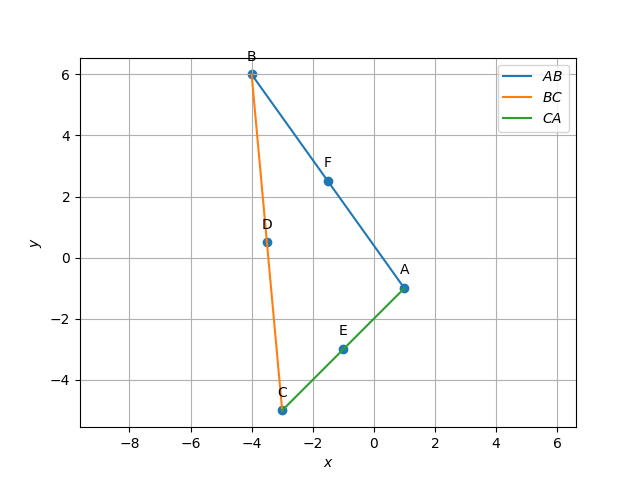
\includegraphics [width=\columnwidth] {./figs/figure.png}
\caption{ The line $\vec{BC}$ plotted using python}
\label{fig: i_line_py}
\end{figure}
\end{document}



\item The area of $\triangle ABC$ is defined as
		\begin{align}
			\frac{1}{2}\norm{{\brak{\vec{A}-\vec{B}}\times {\vec{A}-\vec{C}}}}
		\end{align}
		where
		\begin{align}
			\vec{A}\times\vec{B} \triangleq \mydet{1 & -4 \\-1 & 6}
		\end{align}
		Find the area of $\triangle ABC$.
	\item Find the angles $A, B, C$ if 
    \label{prop:angle2d}
  \begin{align}
    \label{eq:angle2d}
			\cos A \triangleq 
\frac{\brak{\vec{B}-\vec{A}}^{\top}{\vec{C}-\vec{A}}}{\norm{\vec{B}-\vec{A}}\norm{\vec{C}-\vec{A}}}
  \end{align}\\
  	\iffalse
\let\negmedspace\undefined
\let\negthickspace\undefined
\documentclass[journal,12pt,twocolumn]{IEEEtran}
\usepackage{cite}
\usepackage{amsmath,amssymb,amsfonts,amsthm}
\usepackage{algorithmic}
\usepackage{graphicx}
\usepackage{textcomp}
\usepackage{xcolor}
\usepackage{txfonts}
\usepackage{listings}
\usepackage{enumitem}
\usepackage{mathtools}
\usepackage{gensymb}
\usepackage[breaklinks=true]{hyperref}
\usepackage{tkz-euclide} % loads  TikZ and tkz-base
\usepackage{listings}
%\usepackage{gvv}

\newtheorem{theorem}{Theorem}[section]
\newtheorem{problem}{Problem}
\newtheorem{proposition}{Proposition}[section]
\newtheorem{lemma}{Lemma}[section]
\newtheorem{corollary}[theorem]{Corollary}
\newtheorem{example}{Example}[section]
\newtheorem{definition}[problem]{Definition}
\newcommand{\BEQA}{\begin{eqnarray}}
\newcommand{\EEQA}{\end{eqnarray}}
\newcommand{\define}{\stackrel{\triangle}{=}}
\theoremstyle{remark}
\newtheorem{rem}{Remark}

\begin{document}
\bibliographystyle{IEEEtran}
\vspace{3cm}
\title{
%	\logo{
Assignment 1
%	}
}
\author{ Barath Surya M (EE22BTECH11014)}
\maketitle
\newpage
\bigskip
\renewcommand{\thefigure}{\theenumi}
\renewcommand{\thetable}{\theenumi}

\providecommand{\pr}[1]{\ensuremath{\Pr\left(#1\right)}}
\providecommand{\prt}[2]{\ensuremath{p_{#1}^{\left(#2\right)} }}        % own macro for this question
\providecommand{\qfunc}[1]{\ensuremath{Q\left(#1\right)}}
\providecommand{\sbrak}[1]{\ensuremath{{}\left[#1\right]}}
\providecommand{\lsbrak}[1]{\ensuremath{{}\left[#1\right.}}
\providecommand{\rsbrak}[1]{\ensuremath{{}\left.#1\right]}}
\providecommand{\brak}[1]{\ensuremath{\left(#1\right)}}
\providecommand{\lbrak}[1]{\ensuremath{\left(#1\right.}}
\providecommand{\rbrak}[1]{\ensuremath{\left.#1\right)}}
\providecommand{\cbrak}[1]{\ensuremath{\left\{#1\right\}}}
\providecommand{\lcbrak}[1]{\ensuremath{\left\{#1\right.}}
\providecommand{\rcbrak}[1]{\ensuremath{\left.#1\right\}}}
\newcommand{\sgn}{\mathop{\mathrm{sgn}}}
\providecommand{\abs}[1]{\left\vert#1\right\vert}
\providecommand{\res}[1]{\Res\displaylimits_{#1}} 
\providecommand{\norm}[1]{\left\lVert#1\right\rVert}
%\providecommand{\norm}[1]{\lVert#1\rVert}
\providecommand{\mtx}[1]{\mathbf{#1}}
\providecommand{\mean}[1]{E\left[ #1 \right]}
\providecommand{\cond}[2]{#1\middle|#2}
\providecommand{\fourier}{\overset{\mathcal{F}}{ \rightleftharpoons}}
\newenvironment{amatrix}[1]{%
  \left(\begin{array}{@{}*{#1}{c}|c@{}}
}{%
  \end{array}\right)
}
%\providecommand{\hilbert}{\overset{\mathcal{H}}{ \rightleftharpoons}}
%\providecommand{\system}{\overset{\mathcal{H}}{ \longleftrightarrow}}
	%\newcommand{\solution}[2]{\textbf{Solution:}{#1}}
\newcommand{\solution}{\noindent \textbf{Solution: }}
\newcommand{\cosec}{\,\text{cosec}\,}
\providecommand{\dec}[2]{\ensuremath{\overset{#1}{\underset{#2}{\gtrless}}}}
\newcommand{\myvec}[1]{\ensuremath{\begin{pmatrix}#1\end{pmatrix}}}
\newcommand{\mydet}[1]{\ensuremath{\begin{vmatrix}#1\end{vmatrix}}}
\newcommand{\myaugvec}[2]{\ensuremath{\begin{amatrix}{#1}#2\end{amatrix}}}
\providecommand{\rank}{\text{rank}}
\providecommand{\pr}[1]{\ensuremath{\Pr\left(#1\right)}}
\providecommand{\qfunc}[1]{\ensuremath{Q\left(#1\right)}}
	\newcommand*{\permcomb}[4][0mu]{{{}^{#3}\mkern#1#2_{#4}}}
\newcommand*{\perm}[1][-3mu]{\permcomb[#1]{P}}
\newcommand*{\comb}[1][-1mu]{\permcomb[#1]{C}}
\providecommand{\qfunc}[1]{\ensuremath{Q\left(#1\right)}}
\providecommand{\gauss}[2]{\mathcal{N}\ensuremath{\left(#1,#2\right)}}
\providecommand{\diff}[2]{\ensuremath{\frac{d{#1}}{d{#2}}}}
\providecommand{\myceil}[1]{\left \lceil #1 \right \rceil }
\newcommand\figref{Fig.~\ref}
\newcommand\tabref{Table~\ref}
\newcommand{\sinc}{\,\text{sinc}\,}
\newcommand{\rect}{\,\text{rect}\,}
%%
%	%\newcommand{\solution}[2]{\textbf{Solution:}{#1}}
%\newcommand{\solution}{\noindent \textbf{Solution: }}
%\newcommand{\cosec}{\,\text{cosec}\,}
%\numberwithin{equation}{section}
%\numberwithin{equation}{subsection}
%\numberwithin{problem}{section}
%\numberwithin{definition}{section}
%\makeatletter
%\@addtoreset{figure}{problem}
%\makeatother

%\let\StandardTheFigure\thefigure
\let\vec\mathbf





\textbf{Question 1.1.7}
find the angles $\vec{A},\vec{B},\vec{C}$, given that 
\begin{align}
	\cos{A} \triangleq \frac{(\vec{B}-\vec{A})\top(\vec{C}-\vec{A})}{\norm{\vec{B}-\vec{A}}\norm{\vec{C}-\vec{A}}}
\end{align}
\fi
\textbf{Solution}:\\
From the given values of $\vec{A},\vec{B},\vec{C}$,\\
\begin{enumerate}
	\item Finding the value of angle A
\begin{align}
	\vec{B}-\vec{A} &=\myvec{-5\\7}
\end{align}
and 
\begin{align}
	\vec{C}-\vec{A}&= \myvec{-4\\-4}
\end{align}
also calculating the values of norms
\begin{align}
	\norm{\vec{B}-\vec{A}} &= \sqrt{74}\\
	\norm{\vec{C}-\vec{A}} &= \sqrt{32}
\end{align}
and by doing matrix multiplication we get,
\begin{align}
\begin{split}
	(\vec{B}-\vec{A})^{\top}(\vec{C}-\vec{A})&=\myvec{-5&7}\myvec{-4\\-4}\\
	&=-8
\end{split}
\end{align}
so 
\begin{align}
	\cos{A}&= \frac{-8}{\sqrt{74} \sqrt{32}}\\
	&= \frac{-1}{\sqrt{37}}\\
	\implies A&=\cos^{-1}{\frac{-1}{\sqrt{37}}}
\end{align}




\item Finding the value of angle B
\begin{align}
	\vec{C}-\vec{B} &=\myvec{1\\-11}
\end{align}
and 
\begin{align}
	\vec{A}-\vec{B}&= \myvec{5\\-7}
\end{align}
also calculating the values of norms
\begin{align}
	\norm{\vec{C}-\vec{B}} &= \sqrt{122}\\
	\norm{\vec{A}-\vec{B}} &= \sqrt{74}
\end{align}
and by doing matrix multiplication we get,
\begin{align}
\begin{split}
	(\vec{C}-\vec{B})^{\top}(\vec{A}-\vec{B})&=\myvec{1&-11}\myvec{5\\-7}\\
	&= 82
\end{split}
\end{align}
so 
\begin{align}
	\cos{B}&= \frac{82}{\sqrt{74} \sqrt{122}}\\
	&= \frac{41}{\sqrt{2257}}\\
	\implies B&=\cos^{-1}{\frac{41}{\sqrt{2257}}}
\end{align}



\item Finding the value of angle C
\begin{align}
	\vec{A}-\vec{C} &=\myvec{4\\4}
\end{align}
and 
\begin{align}
	\vec{B}-\vec{C}&= \myvec{-1\\11}
\end{align}
also calculating the values of norms
\begin{align}
	\norm{\vec{A}-\vec{C}} &= \sqrt{32}\\
	\norm{\vec{B}-\vec{C}} &= \sqrt{122}
\end{align}
and by doing matrix multiplication we get,
\begin{align}
\begin{split}
	(\vec{A}-\vec{C})^{\top}(\vec{B}-\vec{C})&=\myvec{4&4}\myvec{-1\\11}\\
	&=40
\end{split}
\end{align}
so 
\begin{align}
	\cos{C}&= \frac{40}{\sqrt{32} \sqrt{122}}\\
	&= \frac{5}{\sqrt{61}}\\
	\implies C&=\cos^{-1}{\frac{5}{\sqrt{61}}}
\end{align}

\end{enumerate}

\end{enumerate}

\section{Median}
%\renewcommand{\theequation}{\theenumi}
%\begin{enumerate}[label=\arabic*.,ref=\theenumi]
\begin{enumerate}[label=\thesection.\arabic*.,ref=\thesection.\theenumi]
\numberwithin{equation}{enumi}
\item If $\vec{D}$ divides $BC$ in the ratio $k : 1$,
		\begin{align}
			\vec{D}= \frac{k\vec{C}+\vec{B}}{k+1}
		\end{align}
		Find the mid points $\vec{D}, \vec{E}, \vec{F}$ of the sides $BC, CA$ and $AB$ respectively. 
	\item Find the equations of $AD, BE$ and $CF$.
	\item Find the intersection $\vec{G}$ of $BE$ and $CF$.
	\item Verify that 
		\begin{align}
			\frac{BG}{GE} = 
			\frac{CG}{GF} =
			\frac{AG}{GD} =2 
		\end{align}
	\item Show that $\vec{A}, \vec{G}$ and $\vec{D}$ are collinear.
	\item Verify that 
		\begin{align}
			\vec{G}=\frac{\vec{A}+\vec{B}+\vec{C}}{3}
		\end{align}
			$\vec{G}$ is known as the {\em centroid} of $\triangle ABC$.
	\item Verify that 
		\begin{align}
\vec{A}-\vec{F}=\vec{E}-\vec{D}
		\end{align}
		The quadrilateral $AFDE$ is defined to be a parallelogram.
\end{enumerate}

\section{Altitude}
%\renewcommand{\theequation}{\theenumi}
%\begin{enumerate}[label=\arabic*.,ref=\theenumi]
\begin{enumerate}[label=\thesection.\arabic*.,ref=\thesection.\theenumi]
\numberwithin{equation}{enumi}
\item $\vec{D}_1$ is a point on $BC$ such that
		\begin{align}
			AD_1 \perp BC
		\end{align}
		and $AD_1$ is defined to be the altitude. 
		Find the normal vector of $AD_1$.
	\item Find the equation of $AD_1$.

	\item Find the equations of the altitudes $BE_1$ and $CF_1$ to the sides $AC$ and $AB$ respectively. 
	\item Find the intersection $\vec{H}$ of $BE_1$ and $CF_1$.
	\item Verify that 
		\begin{align}
			\brak{\vec{A}-\vec{H}}^{\top}\brak{\vec{B}-\vec{C}} = 0
		\end{align}
\end{enumerate}

\section{Perpendicular Bisector}
%\renewcommand{\theequation}{\theenumi}
%\begin{enumerate}[label=\arabic*.,ref=\theenumi]
\begin{enumerate}[label=\thesection.\arabic*.,ref=\thesection.\theenumi]
\numberwithin{equation}{enumi}
\item The equation of the perpendicular bisector of $BC$ is
		\begin{align}
			\label{eq:tri-perp-bisect}
			\brak{\vec{x}-\frac{\vec{B}+\vec{C}}{2}}\brak{\vec{B}-\vec{C}} = 0
		\end{align}
		Substitute numerical values and find the equations of the perpendicular bisectors of $AB, BC$ and $CA$.
	\item Find the intersection $\vec{O}$ of the perpendicular bisectors of $AB$ and $AC$.
	\item Verify that $\vec{O}$ satisfies
			\eqref{eq:tri-perp-bisect}.
$\vec{O}$ is known as the circumcentre.
		\item Verify that 
		\begin{align}
			OA = OB = OC 
		\end{align}
	\item Draw the circle with centre at $\vec{O}$ and radius 
		\begin{align}
			R = OA
		\end{align}
		This is known as the {\em circumradius}. 
	\item Verify that 
		\begin{align}
			\angle BOC = 2\angle BAC.
		\end{align}
	\item Let 
		\begin{align}
			\vec{P} = \myvec{\cos \theta & -\sin \theta \\ \sin \theta & \cos \theta}
		\end{align}
		Find $\theta$ if 
		\begin{align}
			\vec{C}-\vec{O}=\vec{P}\brak{\vec{A}-\vec{O}}
		\end{align}
\end{enumerate}

\section{Angle Bisector}
%\renewcommand{\theequation}{\theenumi}
%\begin{enumerate}[label=\arabic*.,ref=\theenumi]
\begin{enumerate}[label=\thesection.\arabic*.,ref=\thesection.\theenumi]
\numberwithin{equation}{enumi}
\item Suppose the equations $AB, BC$ and $CA$ are respectively given by 
		\begin{align}
			\label{eq:tri-sides}
			\vec{n}_i^{\top}\vec{x}=c_i \quad i = 1, 2, 3 
		\end{align}
		The equations of the respective angle bisectors are then given by 
		\begin{align}
			\frac{\vec{n}_i^{\top}\vec{x}-c_i}{\norm{\vec{n}_i}}
		=
	\pm	\frac{\vec{n}_j^{\top}\vec{x}-c_j}{\norm{\vec{n}_j}}
\quad i \ne j
		\end{align}
		Substitute numerical values and find the equations of the angle bisectors of $A, B$ and $C$.
	\\
		\iffalse
\let\negmedspace\undefined
\let\negthickspace\undefined
\documentclass[journal,12pt,twocolumn]{IEEEtran}
\usepackage{cite}
\usepackage{amsmath,amssymb,amsfonts,amsthm}
\usepackage{algorithmic}
\usepackage{graphicx}
\usepackage{textcomp}
\usepackage{xcolor}
\usepackage{txfonts}
\usepackage{listings}
\usepackage{enumitem}
\usepackage{mathtools}
\usepackage{gensymb}
\usepackage[breaklinks=true]{hyperref}
\usepackage{tkz-euclide} % loads  TikZ and tkz-base
\usepackage{listings}
\usepackage{gvv}
%
%\usepackage{setspace}
%\usepackage{gensymb}
%\doublespacing
%\singlespacing

%\usepackage{graphicx}
%\usepackage{amssymb}
%\usepackage{relsize}
%\usepackage[cmex10]{amsmath}
%\usepackage{amsthm}
%\interdisplaylinepenalty=2500
%\savesymbol{iint}
%\usepackage{txfonts}
%\restoresymbol{TXF}{iint}
%\usepackage{wasysym}
%\usepackage{amsthm}
%\usepackage{iithtlc}
%\usepackage{mathrsfs}
%\usepackage{txfonts}
%\usepackage{stfloats}
%\usepackage{bm}
%\usepackage{cite}
%\usepackage{cases}
%\usepackage{subfig}
%\usepackage{xtab}
%\usepackage{longtable}
%\usepackage{multirow}
%\usepackage{algorithm}
%\usepackage{algpseudocode}
%\usepackage{enumitem}
%\usepackage{mathtools}
%\usepackage{tikz}
%\usepackage{circuitikz}
%\usepackage{verbatim}
%\usepackage{tfrupee}
%\usepackage{stmaryrd}
%\usetkzobj{all}
%    \usepackage{color}                                            %%
%    \usepackage{array}                                            %%
%    \usepackage{longtable}                                        %%
%    \usepackage{calc}                                             %%
%    \usepackage{multirow}                                         %%
%    \usepackage{hhline}                                           %%
%    \usepackage{ifthen}                                           %%
  %optionally (for landscape tables embedded in another document): %%
%    \usepackage{lscape}     
%\usepackage{multicol}
%\usepackage{chngcntr}
%\usepackage{enumerate}

%\usepackage{wasysym}
%\documentclass[conference]{IEEEtran}
%\IEEEoverridecommandlockouts
% The preceding line is only needed to identify funding in the first footnote. If that is unneeded, please comment it out.

\newtheorem{theorem}{Theorem}[section]
\newtheorem{problem}{Problem}
\newtheorem{proposition}{Proposition}[section]
\newtheorem{lemma}{Lemma}[section]
\newtheorem{corollary}[theorem]{Corollary}
\newtheorem{example}{Example}[section]
\newtheorem{definition}[problem]{Definition}
%\newtheorem{thm}{Theorem}[section] 
%\newtheorem{defn}[thm]{Definition}
%\newtheorem{algorithm}{Algorithm}[section]
%\newtheorem{cor}{Corollary}
\newcommand{\BEQA}{\begin{eqnarray}}
\newcommand{\EEQA}{\end{eqnarray}}
\newcommand{\define}{\stackrel{\triangle}{=}}
\theoremstyle{remark}
\newtheorem{rem}{Remark}

%\bibliographystyle{ieeetr}
\begin{document}
%

\bibliographystyle{IEEEtran}


\vspace{3cm}

\title{
%	\logo{
ASSIGNMENT-1
%	}
}
\author{ RAMBHA SATVIK - EE22BTECH11043$^{*}$% <-this % stops a space
	\thanks{*The author is with the Department
		of Electrical Engineering, Indian Institute of Technology, Hyderabad
		502285 India e-mail:  ee22btech11043@iith.ac.in. All content in this manual is released under GNU GPL.  Free and open source.}
	
}	
%\title{
%	\logo{Matrix Analysis through Octave}{\begin{center}\includegraphics[scale=.24]{tlc}\end{center}}{}{HAMDSP}
%}


% paper title
% can use linebreaks \\ within to get better formatting as desired
%\title{Matrix Analysis through Octave}
%
%
% author names and IEEE memberships
% note positions of commas and nonbreaking spaces ( ~ ) LaTeX will not break
% a structure at a ~ so this keeps an author's name from being broken across
% two lines.
% use \thanks{} to gain access to the first footnote area
% a separate \thanks must be used for each paragraph as LaTeX2e's \thanks
% was not built to handle multiple paragraphs
%

%\author{<-this % stops a space
%\thanks{}}
%}
% note the % following the last \IEEEmembership and also \thanks - 
% these prevent an unwanted space from occurring between the last author name
% and the end of the author line. i.e., if you had this:
% 
% \author{....lastname \thanks{...} \thanks{...} }
%                     ^------------^------------^----Do not want these spaces!
%
% a space would be appended to the last name and could cause every name on that
% line to be shifted left slightly. This is one of those "LaTeX things". For
% instance, "\textbf{A} \textbf{B}" will typeset as "A B" not "AB". To get
% "AB" then you have to do: "\textbf{A}\textbf{B}"
% \thanks is no different in this regard, so shield the last } of each \thanks
% that ends a line with a % and do not let a space in before the next \thanks.
% Spaces after \IEEEmembership other than the last one are OK (and needed) as
% you are supposed to have spaces between the names. For what it is worth,
% this is a minor point as most people would not even notice if the said evil
% space somehow managed to creep in.



% The paper headers
%\markboth{Journal of \LaTeX\ Class Files,~Vol.~6, No.~1, January~2007}%
%{Shell \MakeLowercase{\textit{et al.}}: Bare Demo of IEEEtran.cls for Journals}
% The only time the second header will appear is for the odd numbered pages
% after the title page when using the twoside option.
% 
% *** Note that you probably will NOT want to include the author's ***
% *** name in the headers of peer review papers.                   ***
% You can use \ifCLASSOPTIONpeerreview for conditional compilation here if
% you desire.




% If you want to put a publisher's ID mark on the page you can do it like
% this:
%\IEEEpubid{0000--0000/00\$00.00~\copyright~2007 IEEE}
% Remember, if you use this you must call \IEEEpubidadjcol in the second
% column for its text to clear the IEEEpubid mark.



% make the title area
\maketitle

\newpage

%\tableofcontents

\bigskip

\renewcommand{\thefigure}{\theenumi}
\renewcommand{\thetable}{\theenumi}
%\renewcommand{\theequation}{\theenumi}

%\begin{abstract}
%%\boldmath
%In this letter, an algorithm for evaluating the exact analytical bit error rate  (BER)  for the piecewise linear (PL) combiner for  multiple relays is presented. Previous results were available only for upto three relays. The algorithm is unique in the sense that  the actual mathematical expressions, that are prohibitively large, need not be explicitly obtained. The diversity gain due to multiple relays is shown through plots of the analytical BER, well supported by simulations. 
%
%\end{abstract}
% IEEEtran.cls defaults to using nonbold math in the Abstract.
% This preserves the distinction between vectors and scalars. However,
% if the journal you are submitting to favors bold math in the abstract,
% then you can use LaTeX's standard command \boldmath at the very start
% of the abstract to achieve this. Many IEEE journals frown on math
% in the abstract anyway.

% Note that keywords are not normally used for peerreview papers.
%\begin{IEEEkeywords}
%Cooperative diversity, decode and forward, piecewise linear
%\end{IEEEkeywords}



% For peer review papers, you can put extra information on the cover
% page as needed:
% \ifCLASSOPTIONpeerreview
% \begin{center} \bfseries EDICS Category: 3-BBND \end{center}
% \fi
%
% For peerreview papers, this IEEEtran command inserts a page break and
% creates the second title. It will be ignored for other modes.
%\IEEEpeerreviewmaketitle

\textbf{Question :} Suppose the equations \textit{AB, BC} and \textit{CA} are respectively given by
		\begin{align}
			\vec{n}_{i}^{\top} \vec{x} = c_{i} \hspace{0.25in} i = 1,2,3
		\end{align}
		The equations of the respective angle bisectors are given by
		\begin{align}
			\frac{\vec{n}_{i}^{\top} \vec{x}-c_{i}}{\norm{\vec{n}_{i}}}=\pm\frac{\vec{n}_{j}^{\top} \vec{x}-c_{j}}{\norm{\vec{n}_{j}}} \hspace{0.25in}i\neq j 
		\end{align}
		Substitute numerical values and find the equations of the angle bisectors of \textit{A,B} and \textit{C}.\\
\fi
\textbf{Solution :}
	The parametric equations of sides;
	\begin{align}
	BC:\quad &\myvec{11&1}\vec{x}=-38,\\
	CA:\quad &\myvec{1&-1}\vec{x}=2,\\
	AB:\quad &\myvec{7&5}\vec{x}=2\\	  
	\end{align}
	Using the formula mentioned in the question to find out the angular bisector for sides \text{AB} and \text{AC}, naming the angular bisector $L$ we get,
	\begin{align}
		\frac{\vec{n}_{3}^{\top} \vec{x}-c_{3}}{\norm{\vec{n}_{3}}}=\pm \frac{\vec{n}_{2}^{\top} \vec{x}-c_{2}}{\norm{\vec{n}_{2}}}
	\end{align}
	\begin{figure}
	\centering
	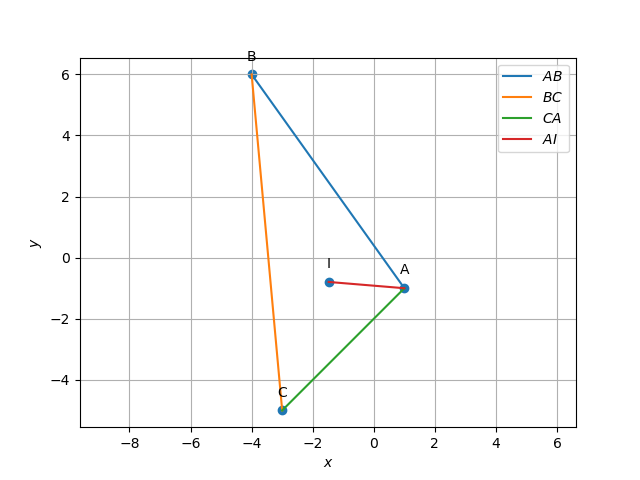
\includegraphics[width=\columnwidth]{solutions/1/5/1/figs/angular_bisector.png}
	\caption{Triangle generated using python}
	\label{fig:angular_bisector}
	\end{figure}
	As we can see we will get 2 solutions for $L$. This is because one of them is internal angular bisector and the other is the external angular bisector. Internal angular bisector can be evaluated if we take + in the above formula.
	Hence, $L$ is given by,
	\begin{align}
		\frac{\vec{n}_{3}^{\top} \vec{x}-c_{3}}{\norm{\vec{n}_{3}}}&=\frac{\vec{n}_{2}^{\top} \vec{x}-c_{2}}{\norm{\vec{n}_{2}}}\\
		\implies \brak{\frac{\vec{n_{3}}}{\norm{\vec{n_{3}}}}-\frac{\vec{n_{3}}}{\norm{\vec{n_{3}}}}} \vec{x}&=\brak{\frac{c_{3}}{\norm{\vec{n_{3}}}}-\frac{c_{2}}{\norm{\vec{n_{2}}}}}\\
		\implies \brak{\frac{\myvec{7&5}}{\sqrt{74}}-\frac{\myvec{1&-1}}{\sqrt{2}}} \vec{x}&=\frac{2}{\sqrt{74}}-\frac{2}{\sqrt{2}}\\
		\implies \myvec{\frac{7-\sqrt{37}}{\sqrt{74}}&\frac{5+\sqrt{37}}{\sqrt{74}}}\vec{x}&=\frac{2-2\sqrt{37}}{\sqrt{74}}
	\end{align}
	Hence, the internal angluar bisector of angle $A$, $L$ will be,
	\begin{align}
		\implies\myvec{\frac{7-\sqrt{37}}{\sqrt{74}}&\frac{5+\sqrt{37}}{\sqrt{74}}} \vec{x}=\frac{2-2\sqrt{37}}{\sqrt{74}}
		\label{eq:1.5.1}
	\end{align}
	

	\item Find the intersection $\vec{I}$ of the angle bisectors of $B$ and $C$.
 \\
		\documentclass[journal,12pt,twocolumn]{IEEEtran}
\usepackage{cite}
\usepackage{amsmath,amssymb,amsfonts,amsthm}
\usepackage{algorithmic}
\usepackage{graphicx}
\usepackage{textcomp}
\usepackage{xcolor}
\usepackage{txfonts}
\usepackage{listings}
\usepackage{enumitem}
\usepackage{mathtools}
\usepackage{gensymb}
\usepackage[breaklinks=true]{hyperref}
\usepackage{tkz-euclide} % loads  TikZ and tkz-base
\usepackage{listings}
\usepackage{float}


\begin{document}
\providecommand{\pr}[1]{\ensuremath{\Pr\left(#1\right)}}
\providecommand{\prt}[2]{\ensuremath{p_{#1}^{\left(#2\right)} }}        % own macro for this question
\providecommand{\qfunc}[1]{\ensuremath{Q\left(#1\right)}}
\providecommand{\sbrak}[1]{\ensuremath{{}\left[#1\right]}}
\providecommand{\lsbrak}[1]{\ensuremath{{}\left[#1\right.}}
\providecommand{\rsbrak}[1]{\ensuremath{{}\left.#1\right]}}
\providecommand{\brak}[1]{\ensuremath{\left(#1\right)}}
\providecommand{\lbrak}[1]{\ensuremath{\left(#1\right.}}
\providecommand{\rbrak}[1]{\ensuremath{\left.#1\right)}}
\providecommand{\cbrak}[1]{\ensuremath{\left\{#1\right\}}}
\providecommand{\lcbrak}[1]{\ensuremath{\left\{#1\right.}}
\providecommand{\rcbrak}[1]{\ensuremath{\left.#1\right\}}}
\newcommand{\sgn}{\mathop{\mathrm{sgn}}}
\providecommand{\abs}[1]{\left\vert#1\right\vert}
\providecommand{\res}[1]{\Res\displaylimits_{#1}} 
\providecommand{\norm}[1]{\left\lVert#1\right\rVert}
%\providecommand{\norm}[1]{\lVert#1\rVert}
\providecommand{\mtx}[1]{\mathbf{#1}}
\providecommand{\mean}[1]{E\left[ #1 \right]}
\providecommand{\cond}[2]{#1\middle|#2}
\providecommand{\fourier}{\overset{\mathcal{F}}{ \rightleftharpoons}}
\newenvironment{amatrix}[1]{%
  \left(\begin{array}{@{}*{#1}{c}|c@{}}
}{%
  \end{array}\right)
}
%\providecommand{\hilbert}{\overset{\mathcal{H}}{ \rightleftharpoons}}
%\providecommand{\system}{\overset{\mathcal{H}}{ \longleftrightarrow}}
	%\newcommand{\solution}[2]{\textbf{Solution:}{#1}}
\newcommand{\solution}{\noindent \textbf{Solution: }}
\newcommand{\cosec}{\,\text{cosec}\,}
\providecommand{\dec}[2]{\ensuremath{\overset{#1}{\underset{#2}{\gtrless}}}}
\newcommand{\myvec}[1]{\ensuremath{\begin{pmatrix}#1\end{pmatrix}}}
\newcommand{\mydet}[1]{\ensuremath{\begin{vmatrix}#1\end{vmatrix}}}
\newcommand{\myaugvec}[2]{\ensuremath{\begin{amatrix}{#1}#2\end{amatrix}}}
\providecommand{\rank}{\text{rank}}
\providecommand{\pr}[1]{\ensuremath{\Pr\left(#1\right)}}
\providecommand{\qfunc}[1]{\ensuremath{Q\left(#1\right)}}
	\newcommand*{\permcomb}[4][0mu]{{{}^{#3}\mkern#1#2_{#4}}}
\newcommand*{\perm}[1][-3mu]{\permcomb[#1]{P}}
\newcommand*{\comb}[1][-1mu]{\permcomb[#1]{C}}
\providecommand{\qfunc}[1]{\ensuremath{Q\left(#1\right)}}
\providecommand{\gauss}[2]{\mathcal{N}\ensuremath{\left(#1,#2\right)}}
\providecommand{\diff}[2]{\ensuremath{\frac{d{#1}}{d{#2}}}}
\providecommand{\myceil}[1]{\left \lceil #1 \right \rceil }
\newcommand\figref{Fig.~\ref}
\newcommand\tabref{Table~\ref}
\newcommand{\sinc}{\,\text{sinc}\,}
\newcommand{\rect}{\,\text{rect}\,}
%%
%	%\newcommand{\solution}[2]{\textbf{Solution:}{#1}}
%\newcommand{\solution}{\noindent \textbf{Solution: }}
%\newcommand{\cosec}{\,\text{cosec}\,}
%\numberwithin{equation}{section}
%\numberwithin{equation}{subsection}
%\numberwithin{problem}{section}
%\numberwithin{definition}{section}
%\makeatletter
%\@addtoreset{figure}{problem}
%\makeatother

%\let\StandardTheFigure\thefigure
\let\vec\mathbf

\bibliographystyle{IEEEtran}


\vspace{3cm}

Question 1.5.2\\
Find the intersection $\vec{I}$ of the angle bisectors of $\vec{B}$ and $\vec{C}$
\fi
Solution:\\
From \ref{eq:1.5.1} the bisectors of $\vec{B}$ and $\vec{C}$ are obtained as 
\begin{align}
\myvec{
\frac{11}{\sqrt{122}}+\frac{7}{\sqrt{74}} & \frac{1}{\sqrt{122}}+\frac{5}{\sqrt{74}}\\
}
\vec{x}
=\frac{2}{\sqrt{74}}-\frac{38}{\sqrt{122}}
\end{align}
and 
\begin{align}
\myvec{
\frac{11}{\sqrt{122}}+\frac{1}{\sqrt{2}} & \frac{1}{\sqrt{122}}-\frac{1}{\sqrt{2}}\\
}
\vec{x}
=\frac{2}{\sqrt{2}}-\frac{38}{\sqrt{122}}
\end{align}
respectively.
The pair of linear equations can be solved using the Augmented matrix $\myvec{
\vec{P}|\vec{Q}}$
Here,
\begin{align}
\vec{P}&=\myvec{
\frac{11}{\sqrt{122}}+\frac{7}{\sqrt{74}} & \frac{1}{\sqrt{122}}+\frac{5}{\sqrt{74}}\\
\frac{11}{\sqrt{122}}+\frac{1}{\sqrt{2}} & \frac{1}{\sqrt{122}}-\frac{1}{\sqrt{2}}\\
}\\
\vec{Q}&=\myvec{
\frac{2}{\sqrt{74}}-\frac{38}{\sqrt{122}}\
\frac{2}{\sqrt{2}}-\frac{38}{\sqrt{122}}\\
}\\
\myaugvec{1}{\vec{P}&\vec{Q}} 
 &= \myaugvec{2}
 {
\frac{11}{\sqrt{122}}+\frac{7}{\sqrt{74}} & \frac{1}{\sqrt{122}}+\frac{5}{\sqrt{74}} & \frac{2}{\sqrt{74}}-\frac{38}{\sqrt{122}} \\
\frac{11}{\sqrt{122}}+\frac{1}{\sqrt{2}} & \frac{1}{\sqrt{122}}-\frac{1}{\sqrt{2}} & \frac{2}{\sqrt{2}}-\frac{38}{\sqrt{122}} \\
}
\end{align}
The augmented matrix is converted into decimal notations for easier calculations and then can be solved using row reduction as follows 
\begin{align}
\myaugvec{2}
{
1.81 & 0.67 & -3.21 \\
 1.7 & -0.62 & -2.03\\
}
 \xleftrightarrow[]{R_2\leftarrow 1.7R_1-1.81R_2}
\myaugvec{2}
{1.81 & 0.67 & -3.21 \\
0 & 1.33 & -1.05\\
}\\
\xleftrightarrow[]{R_1\leftarrow 1.33R_1-0.67R_2}
\myaugvec{2}
{1.81 & 0 & -2.68 \\
0 & 1.33 & -1.05\\
}\\
\xleftrightarrow[]{R_1\leftarrow \frac{R_1}{1.81}}
\myaugvec{2}
{
1 & 0 & -1.48 \\
0 & 1.33 & -1.05\\
}\\
\xleftrightarrow[]{R_2\leftarrow \frac{R_2}{1.33}}
\myaugvec{2}{1 & 0 & -1.48 \\ 0 & 1 & -0.79} 
\end{align}
We obtain 
\begin{align}
\vec{I}=\myvec{-1.48\\-0.79}
\end{align}
\begin{figure}[H]
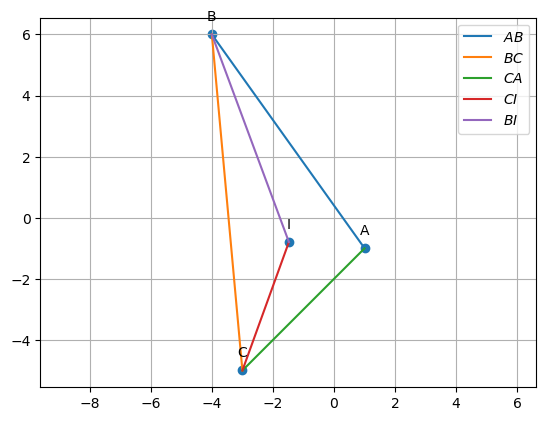
\includegraphics[width=\columnwidth]{./figs/Incentre.png}
\caption{Intersection point $\vec{I}$ of angle bisectors of $\vec{B}$and$\vec{C}$ plotted using python}
\label{fig:i_tri_py}
\end{figure}



	\item Using 
    \eqref{eq:angle2d}
verify that 
		\begin{align}
			\angle BAI = \angle CAI.
		\end{align}
	\item Find the distance from $\vec{I}$ to $BC$.  
	\item Repeat the above exercise for the sides $AB$ and $AC$.
	\item This distance is known as the {\em inradius} $r$.
	\item Draw a circle with center $\vec{I}$ and radius $r$.  $\vec{I}$ is known as the {\em incentre}.
	\item The equation of the {\em incircle} is given by 
		\begin{align}
			\norm{\vec{x}-\vec{I}}^2 = r^2
		\end{align}
		Find the parameteric equation of $BC$ and use it to verify that $BC$ intersects the incircle at exactly one point $\vec{D}_3$.  $BC$ is defined to be a {\em tangent} to the incircle.  $\vec{D}_3$ is defined to be {\em point of contact}.
	\\
		\iffalse
\documentclass[journal,12pt,twocolumn]{IEEEtran}
\usepackage{cite}
\usepackage{amsmath,amssymb,amsfonts,amsthm}
\usepackage{algorithmic}
\usepackage{graphicx}
\usepackage{textcomp}
\usepackage{xcolor}
\usepackage{txfonts}
\usepackage{listings}
\usepackage{enumitem}
\usepackage{mathtools}
\usepackage{gensymb}
\usepackage[breaklinks=true]{hyperref}
\usepackage{tkz-euclide} % loads  TikZ and tkz-base
\usepackage{listings}
\usepackage{float}


\begin{document}
\providecommand{\pr}[1]{\ensuremath{\Pr\left(#1\right)}}
\providecommand{\prt}[2]{\ensuremath{p_{#1}^{\left(#2\right)} }}        % own macro for this question
\providecommand{\qfunc}[1]{\ensuremath{Q\left(#1\right)}}
\providecommand{\sbrak}[1]{\ensuremath{{}\left[#1\right]}}
\providecommand{\lsbrak}[1]{\ensuremath{{}\left[#1\right.}}
\providecommand{\rsbrak}[1]{\ensuremath{{}\left.#1\right]}}
\providecommand{\brak}[1]{\ensuremath{\left(#1\right)}}
\providecommand{\lbrak}[1]{\ensuremath{\left(#1\right.}}
\providecommand{\rbrak}[1]{\ensuremath{\left.#1\right)}}
\providecommand{\cbrak}[1]{\ensuremath{\left\{#1\right\}}}
\providecommand{\lcbrak}[1]{\ensuremath{\left\{#1\right.}}
\providecommand{\rcbrak}[1]{\ensuremath{\left.#1\right\}}}
\newcommand{\sgn}{\mathop{\mathrm{sgn}}}
\providecommand{\abs}[1]{\left\vert#1\right\vert}
\providecommand{\res}[1]{\Res\displaylimits_{#1}} 
\providecommand{\norm}[1]{\left\lVert#1\right\rVert}
%\providecommand{\norm}[1]{\lVert#1\rVert}
\providecommand{\mtx}[1]{\mathbf{#1}}
\providecommand{\mean}[1]{E\left[ #1 \right]}
\providecommand{\cond}[2]{#1\middle|#2}
\providecommand{\fourier}{\overset{\mathcal{F}}{ \rightleftharpoons}}
\newenvironment{amatrix}[1]{%
  \left(\begin{array}{@{}*{#1}{c}|c@{}}
}{%
  \end{array}\right)
}
%\providecommand{\hilbert}{\overset{\mathcal{H}}{ \rightleftharpoons}}
%\providecommand{\system}{\overset{\mathcal{H}}{ \longleftrightarrow}}
	%\newcommand{\solution}[2]{\textbf{Solution:}{#1}}
\newcommand{\solution}{\noindent \textbf{Solution: }}
\newcommand{\cosec}{\,\text{cosec}\,}
\providecommand{\dec}[2]{\ensuremath{\overset{#1}{\underset{#2}{\gtrless}}}}
\newcommand{\myvec}[1]{\ensuremath{\begin{pmatrix}#1\end{pmatrix}}}
\newcommand{\mydet}[1]{\ensuremath{\begin{vmatrix}#1\end{vmatrix}}}
\newcommand{\myaugvec}[2]{\ensuremath{\begin{amatrix}{#1}#2\end{amatrix}}}
\providecommand{\rank}{\text{rank}}
\providecommand{\pr}[1]{\ensuremath{\Pr\left(#1\right)}}
\providecommand{\qfunc}[1]{\ensuremath{Q\left(#1\right)}}
	\newcommand*{\permcomb}[4][0mu]{{{}^{#3}\mkern#1#2_{#4}}}
\newcommand*{\perm}[1][-3mu]{\permcomb[#1]{P}}
\newcommand*{\comb}[1][-1mu]{\permcomb[#1]{C}}
\providecommand{\qfunc}[1]{\ensuremath{Q\left(#1\right)}}
\providecommand{\gauss}[2]{\mathcal{N}\ensuremath{\left(#1,#2\right)}}
\providecommand{\diff}[2]{\ensuremath{\frac{d{#1}}{d{#2}}}}
\providecommand{\myceil}[1]{\left \lceil #1 \right \rceil }
\newcommand\figref{Fig.~\ref}
\newcommand\tabref{Table~\ref}
\newcommand{\sinc}{\,\text{sinc}\,}
\newcommand{\rect}{\,\text{rect}\,}
%%
%	%\newcommand{\solution}[2]{\textbf{Solution:}{#1}}
%\newcommand{\solution}{\noindent \textbf{Solution: }}
%\newcommand{\cosec}{\,\text{cosec}\,}
%\numberwithin{equation}{section}
%\numberwithin{equation}{subsection}
%\numberwithin{problem}{section}
%\numberwithin{definition}{section}
%\makeatletter
%\@addtoreset{figure}{problem}
%\makeatother

%\let\StandardTheFigure\thefigure
\let\vec\mathbf

\bibliographystyle{IEEEtran}


\vspace{3cm}


\title{
Probability Assignment 1	}
}
\author{EE22BTECH11052 - SUJAL GUPTA
	
}	
%\title{
%	\logo{Matrix Analysis through Octave}{\begin{center}\includegraphics[scale=.24]{tlc}\end{center}}{}{HAMDSP}
%}


% paper title
% can use linebreaks \\ within to get better formatting as desired
%\title{Matrix Analysis through Octave}
%
%
% author names and IEEE memberships
% note positions of commas and nonbreaking spaces ( ~ ) LaTeX will not break
% a structure at a ~ so this keeps an author's name from being broken across
% two lines.
% use \thanks{} to gain access to the first footnote area
% a separate \thanks must be used for each paragraph as LaTeX2e's \thanks
% was not built to handle multiple paragraphs
%

%\author{<-this % stops a space
%\thanks{}}
%}
% note the % following the last \IEEEmembership and also \thanks - 
% these prevent an unwanted space from occurring between the last author name
% and the end of the author line. i.e., if you had this:
% 
% \author{....lastname \thanks{...} \thanks{...} }
%                     ^------------^------------^----Do not want these spaces!
%
% a space would be appended to the last name and could cause every name on that
% line to be shifted left slightly. This is one of those "LaTeX things". For
% instance, "\textbf{A} \textbf{B}" will typeset as "A B" not "AB". To get
% "AB" then you have to do: "\textbf{A}\textbf{B}"
% \thanks is no different in this regard, so shield the last } of each \thanks
% that ends a line with a % and do not let a space in before the next \thanks.
% Spaces after \IEEEmembership other than the last one are OK (and needed) as
% you are supposed to have spaces between the names. For what it is worth,
% this is a minor point as most people would not even notice if the said evil
% space somehow managed to creep in.



% The paper headers
%\markboth{Journal of \LaTeX\ Class Files,~Vol.~6, No.~1, January~2007}%
%{Shell \MakeLowercase{\textit{et al.}}: Bare Demo of IEEEtran.cls for Journals}
% The only time the second header will appear is for the odd numbered pages
% after the title page when using the twoside option.
% 
% *** Note that you probably will NOT want to include the author's ***
% *** name in the headers of peer review papers.                   ***
% You can use \ifCLASSOPTIONpeerreview for conditional compilation here if
% you desire.




% If you want to put a publisher's ID mark on the page you can do it like
% this:
%\IEEEpubid{0000--0000/00\$00.00~\copyright~2007 IEEE}
% Remember, if you use this you must call \IEEEpubidadjcol in the second
% column for its text to clear the IEEEpubid mark.



% make the title area
\maketitle

\newpage

%\tableofcontents

\bigskip

\renewcommand{\thefigure}{\theenumi}
\renewcommand{\thetable}{\theenumi}
%\renewcommand{\theequation}{\theenumi}

%\begin{abstract}
%%\boldmath
%In this letter, an algorithm for evaluating the exact analytical bit error rate  (BER)  for the piecewise linear (PL) combiner for  multiple relays is presented. Previous results were available only for upto three relays. The algorithm is unique in the sense that  the actual mathematical expressions, that are prohibitively large, need not be explicitly obtained. The diversity gain due to multiple relays is shown through plots of the analytical BER, well supported by simulations. 
%
%\end{abstract}
% IEEEtran.cls defaults to using nonbold math in the Abstract.
% This preserves the distinction between vectors and scalars. However,
% if the journal you are submitting to favors bold math in the abstract,
% then you can use LaTeX's standard command \boldmath at the very start
% of the abstract to achieve this. Many IEEE journals frown on math
% in the abstract anyway.

% Note that keywords are not normally used for peerreview papers.
%\begin{IEEEkeywords}
%Cooperative diversity, decode and forward, piecewise linear
%\end{IEEEkeywords}



% For peer review papers, you can put extra information on the cover
% page as needed:
% \ifCLASSOPTIONpeerreview
% \begin{center} \bfseries EDICS Category: 3-BBND \end{center}
% \fi
%
% For peerreview papers, this IEEEtran command inserts a page break and
% creates the second title. It will be ignored for other modes.
%\IEEEpeerreviewmaketitle

%\begin{abstract}
%his manual includes \LaTeX figures.
%book provides an introduction to optimization  based on the NCERT textbooks from Class 6-12.  Links to sample Python codes are available in the text.  
%\end{abstract}
%Download 
%\begin{lstlisting}
%svn co https://github.com/gadepall/school/trunk/training
%\end{lstlisting}

%\renewcommand{\theequation}{\theenumi}
%\subsection{Problem}

%\section{Chemistry}
%\begin{enumerate}[label=\arabic*.,ref=\thesection.\theenumi]
%\numberwithin{equation}{enumi}
Given in the question:
% \begin{description}
  % \item 
  \begin{align}
    \vec{A} &= \myvec{1\\-1}  ,\\
  % \item 
    \vec{B} &= \myvec{-4\\6} ,\\
  % \item 
    \vec{C} &= \myvec{-3\\-5}
    \end{align}
% \end{description}

The equation of the incircle is given by
\begin{align}
\norm{\vec{x}-\vec{I}}^2 = r^2
\end{align}
Find the parameteric equation of $BC$ and use it to verify that $BC$
intersects the incircle at exactly one point $\vec{D_{3}}$ . $BC$ is defined to be a
tangent to the incircle. $\vec{D_{3}}$ is defined to be point of contact.
\fi
\solution
Let us define 
\begin{align}
\vec{m} = \vec{C}-\vec{B} 
\end{align}
and $\vec{I}$ is the incentre of the $\triangle ABC$

\begin{align}
\vec{I} &= \frac{1}{\sqrt{74}+\sqrt{32}+\sqrt{122}}\myvec{{\sqrt{122}-4\sqrt{32}-3\sqrt{74}}\\{-\sqrt{122}+6\sqrt{32}-5\sqrt{74}}}\\
&=\myvec{-1.47756217 \\-0.79495069}
\end{align}
The general position vector on the line $BC$ (in parametric form)  and the equation of incircle are:
\begin{align}
\vec{x} &= \vec{B} + k{\vec{m}}\label{eq:8}\\
\norm{\ \vec{x} - \vec{I}\ }^2 &= r^2 \label{eq:9}
\end{align}
Substituting the value of $ \vec{x} $ from \eqref{eq:8} in \eqref{eq:9}
\begin{align}
  \norm{ \vec{B} + k{\vec{m}}- \vec{I} }^2 &= r^2 \\
  \sbrak{\vec{B} + k{\vec{m}}- \vec{I}}^{\top} \sbrak{\vec{B} + k{\vec{m}}- \vec{I}} &= r^2 
\end{align}
On simplifying the above equation:
\begin{multline}
k^2\norm{\vec{m}}^2 +2k{\vec{m}^{\top}}\brak{{\vec{B}-\vec{I}}}+\norm{\vec{I}}^2 +\norm{\vec{B}}^2\\-2\brak{\vec{B}^{\top}\vec{I}} - r^2=0
\end{multline}
The above is a quadratic equation in $k$.
The Discriminant of the quadratic equation is:
\begin{multline}
D = {\cbrak{2\sbrak{\vec{m}^{\top}\brak{\vec{B}-\vec{I}}}}}^2-4(\ \norm{\vec{m}}^2)(\ \norm{\vec{I}}^2 +\norm{\vec{B}}^2\\-2\brak{\vec{B}^{\top}\vec{I}} - r^2)\\
= {\sbrak{2\myvec{1&-11}\myvec{-4+1.47756217\\6+0.79495069}}}^2 \\-4[122][2.8151+52-2(1.140544)\\-3.59820]\\
=4\sbrak{{\brak{-2.522-74.744}}^2-5970.173}\\
=4[5970.173121-5970.173121]\\
=0
\end{multline}
%\end{multline}
%\begin{multline}
%\begin{align}

We substituted the values of $\vec{B},\vec{I},\vec{m}$
On solving this Discriminant turns out to be zero.
Hence, the quadratic equation has only one solution.
To find the unique solution of the equation (i.e. the unique value of $k$), Set discriminant value to 0.
And the solution is \begin{align}k=\frac{-2\vec{m}^{\top}\brak{\vec{B}-\vec{I}}}{2{\ \norm{\vec{m}}^2}}\end{align}

On substituting the values, the value of $k$ is 
\begin{align}
k&=-\myvec{1&-11}\myvec{-4-\frac{\sqrt{122}-4\sqrt{32}-3\sqrt{74}}{\sqrt{74}+\sqrt{32}+\sqrt{122}}\\6-\frac{-\sqrt{122}+6\sqrt{32}-5\sqrt{74}}{\sqrt{74}+\sqrt{32}+\sqrt{122}}}\\
&=\myvec{1&-11}\myvec{\frac{5\sqrt{122}+\sqrt{74}}{\sqrt{74}+\sqrt{32}+\sqrt{122}}\\\frac{-7\sqrt{122}-11\sqrt{74}}{\sqrt{74}+\sqrt{32}+\sqrt{122}}}\\
&=\frac{122\sqrt{74}+82\sqrt{122}}{122(\sqrt{74}+\sqrt{122}+\sqrt{32})}\\
&=0.6333352080102638
\end{align}

So on substituting this value in \eqref{eq:8}, we get the point $\vec{D_{3}}$ 
\begin{align}
\vec{D_{3}} &=\myvec{-4\\6} + \frac{122\sqrt{74}+82\sqrt{122}}{122\brak{\sqrt{74}+\sqrt{122}+\sqrt{32}}}\myvec{1\\-11}\\
&=\myvec{-4+\frac{122\sqrt{74}+82\sqrt{122}}{122\brak{\sqrt{74}+\sqrt{122}+\sqrt{32}}}\\6-11\frac{122\sqrt{74}+82\sqrt{122}}{122\brak{\sqrt{74}+\sqrt{122}+\sqrt{32}}}}\\
&=\myvec{{\frac{-366\sqrt{74}-406\sqrt{122}-488\sqrt{32}}{122\brak{\sqrt{74}+\sqrt{32}+\sqrt{122}}}}\\{\frac{-610\sqrt{74}+732\sqrt{32}-170\sqrt{122}}{122\brak{\sqrt{74}+\sqrt{32}+\sqrt{122}}}}}\\
&=\myvec{-3.36666479\\-0.96668729}
\end{align}

\begin{figure}[H]
\centering
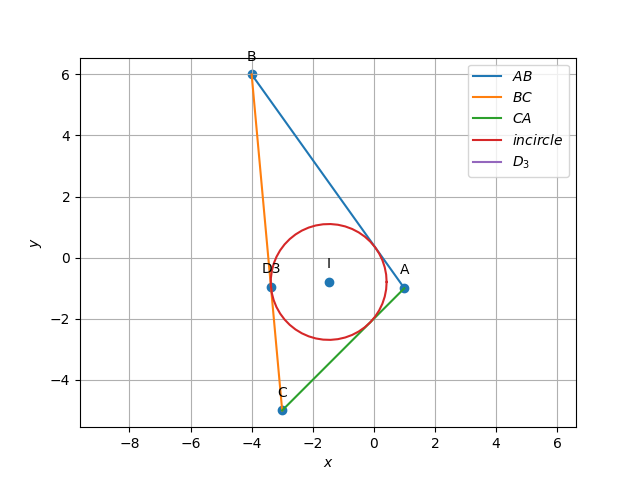
\includegraphics[width=\columnwidth]{solutions/1/5/8/figs/incircle.png}
\caption{Incircle generated using python}
\label{fig:Incircle_py}
\end{figure}

  \item Find the other points of contact $\vec{E}_3$ and $\vec{F}_3$.
	\item Verify that 
		\begin{align}
			AE_3 = AF_3=m, BD_3 = BF_3=n, CD_3 = CE_3=p.
		\end{align}
	\item Obtain $m,n,p$ in terms of $a,b,c$, the sides of the triangle using a matrix equation.  Obtain the numerical values.
 \\
 		
\let\negmedspace\undefined
\let\negthickspace\undefined
\documentclass[journal,12pt,twocolumn]{IEEEtran}
\usepackage{cite}
\usepackage{amsmath,amssymb,amsfonts,amsthm}
\usepackage{algorithmic}
\usepackage{graphicx}
\usepackage{textcomp}
\usepackage{xcolor}
\usepackage{txfonts}
\usepackage{listings}
\usepackage{enumitem}
\usepackage{mathtools}
\usepackage{gensymb}
\usepackage[breaklinks=true]{hyperref}
\usepackage{tkz-euclide} % loads  TikZ and tkz-base
\usepackage{listings}
\usepackage{gvv}
%
%\usepackage{setspace}
%\usepackage{gensymb}
%\doublespacing
%\singlespacing

%\usepackage{graphicx}
%\usepackage{amssymb}
%\usepackage{relsize}
%\usepackage[cmex10]{amsmath}
%\usepackage{amsthm}
%\interdisplaylinepenalty=2500
%\savesymbol{iint}
%\usepackage{txfonts}
%\restoresymbol{TXF}{iint}
%\usepackage{wasysym}
%\usepackage{amsthm}
%\usepackage{iithtlc}
%\usepackage{mathrsfs}
%\usepackage{txfonts}
%\usepackage{stfloats}
%\usepackage{bm}
%\usepackage{cite}
%\usepackage{cases}
%\usepackage{subfig}
%\usepackage{xtab}
%\usepackage{longtable}
%\usepackage{multirow}
%\usepackage{algorithm}
%\usepackage{algpseudocode}
%\usepackage{enumitem}
%\usepackage{mathtools}
%\usepackage{tikz}
%\usepackage{circuitikz}
%\usepackage{verbatim}
%\usepackage{tfrupee}
%\usepackage{stmaryrd}
%\usetkzobj{all}
%    \usepackage{color}                                            %%
%    \usepackage{array}                                            %%
%    \usepackage{longtable}                                        %%
%    \usepackage{calc}                                             %%
%    \usepackage{multirow}                                         %%
%    \usepackage{hhline}                                           %%
%    \usepackage{ifthen}                                           %%
  %optionally (for landscape tables embedded in another document): %%
%    \usepackage{lscape}     
%\usepackage{multicol}
%\usepackage{chngcntr}
%\usepackage{enumerate}

%\usepackage{wasysym}
%\documentclass[conference]{IEEEtran}
%\IEEEoverridecommandlockouts
% The preceding line is only needed to identify funding in the first footnote. If that is unneeded, please comment it out.

\newtheorem{theorem}{Theorem}[section]
\newtheorem{problem}{Problem}
\newtheorem{proposition}{Proposition}[section]
\newtheorem{lemma}{Lemma}[section]
\newtheorem{corollary}[theorem]{Corollary}
\newtheorem{example}{Example}[section]
\newtheorem{definition}[problem]{Definition}
%\newtheorem{thm}{Theorem}[section] 
%\newtheorem{defn}[thm]{Definition}
%\newtheorem{algorithm}{Algorithm}[section]
%\newtheorem{cor}{Corollary}
\newcommand{\BEQA}{\begin{eqnarray}}
\newcommand{\EEQA}{\end{eqnarray}}
\newcommand{\define}{\stackrel{\triangle}{=}}
\theoremstyle{remark}
\newtheorem{rem}{Remark}

%\bibliographystyle{ieeetr}
\begin{document}
%

\bibliographystyle{IEEEtran}


\vspace{3cm}

\title{
    Solution to problem number 1.5.11
}
\author{ Yash Patil - EE22BTECH11058}
%\title{
%	\logo{Matrix Analysis through Octave}{\begin{center}\includegraphics[scale=.24]{tlc}\end{center}}{}{HAMDSP}
%}


% paper title
% can use linebreaks \\ within to get better formatting as desired
%\title{Matrix Analysis through Octave}
%
%
% author names and IEEE memberships
% note positions of commas and nonbreaking spaces ( ~ ) LaTeX will not break
% a structure at a ~ so this keeps an author's name from being broken across
% two lines.
% use \thanks{} to gain access to the first footnote area
% a separate \thanks must be used for each paragraph as LaTeX2e's \thanks
% was not built to handle multiple paragraphs
%

%\author{<-this % stops a space
%\thanks{}}
%}
% note the % following the last \IEEEmembership and also \thanks - 
% these prevent an unwanted space from occurring between the last author name
% and the end of the author line. i.e., if you had this:
% 
% \author{....lastname \thanks{...} \thanks{...} }
%                     ^------------^------------^----Do not want these spaces!
%
% a space would be appended to the last name and could cause every name on that
% line to be shifted left slightly. This is one of those "LaTeX things". For
% instance, "\textbf{A} \textbf{B}" will typeset as "A B" not "AB". To get
% "AB" then you have to do: "\textbf{A}\textbf{B}"
% \thanks is no different in this regard, so shield the last } of each \thanks
% that ends a line with a % and do not let a space in before the next \thanks.
% Spaces after \IEEEmembership other than the last one are OK (and needed) as
% you are supposed to have spaces between the names. For what it is worth,
% this is a minor point as most people would not even notice if the said evil
% space somehow managed to creep in.



% The paper headers
%\markboth{Journal of \LaTeX\ Class Files,~Vol.~6, No.~1, January~2007}%
%{Shell \MakeLowercase{\textit{et al.}}: Bare Demo of IEEEtran.cls for Journals}
% The only time the second header will appear is for the odd numbered pages
% after the title page when using the twoside option.
% 
% *** Note that you probably will NOT want to include the author's ***
% *** name in the headers of peer review papers.                   ***
% You can use \ifCLASSOPTIONpeerreview for conditional compilation here if
% you desire.




% If you want to put a publisher's ID mark on the page you can do it like
% this:
%\IEEEpubid{0000--0000/00\$00.00~\copyright~2007 IEEE}
% Remember, if you use this you must call \IEEEpubidadjcol in the second
% column for its text to clear the IEEEpubid mark.



% make the title area
\maketitle

\newpage

%\tableofcontents

\bigskip

\renewcommand{\thefigure}{\theenumi}
\renewcommand{\thetable}{\theenumi}
%\renewcommand{\theequation}{\theenumi}

%\begin{abstract}
%%\boldmath
%In this letter, an algorithm for evaluating the exact analytical bit error rate  (BER)  for the piecewise linear (PL) combiner for  multiple relays is presented. Previous results were available only for upto three relays. The algorithm is unique in the sense that  the actual mathematical expressions, that are prohibitively large, need not be explicitly obtained. The diversity gain due to multiple relays is shown through plots of the analytical BER, well supported by simulations. 
%
%\end{abstract}
% IEEEtran.cls defaults to using nonbold math in the Abstract.
% This preserves the distinction between vectors and scalars. However,
% if the journal you are submitting to favors bold math in the abstract,
% then you can use LaTeX's standard command \boldmath at the very start
% of the abstract to achieve this. Many IEEE journals frown on math
% in the abstract anyway.

% Note that keywords are not normally used for peerreview papers.
%\begin{IEEEkeywords}
%Cooperative diversity, decode and forward, piecewise linear
%\end{IEEEkeywords}



% For peer review papers, you can put extra information on the cover
% page as needed:
% \ifCLASSOPTIONpeerreview
% \begin{center} \bfseries EDICS Category: 3-BBND \end{center}
% \fi
%
% For peerreview papers, this IEEEtran command inserts a page break and
% creates the second title. It will be ignored for other modes.
%\IEEEpeerreviewmaketitle
\textbf{Question:}
Obtain p, q, r in terms of a, b, c, the sides of the triangle using a matrix
equation. Obtain the numerical values.\\
\indent\textbf{Solution:}
Given in the question:
\begin{align}
    \vec{A} &= \myvec{ 1 \\ -1 }\\
    \vec{B} &= \myvec{ -4 \\ 6 }\\
    \vec{C} &= \myvec{ -3 \\ -5 } 
\end{align}
Now, the side lengths a, b and c can be calculated as:
\begin{align}
    a &= \sqrt{(\vec{C}-\vec{B})^{\top}(\vec{C}-\vec{B})}\\
    &= \sqrt{\myvec{1&-11} \myvec{1\\-11}}\\
    &= \sqrt{1+121}\\
    &=\sqrt{122}    \\
    b &= \sqrt{(\vec{A}-\vec{C})^{\top}(\vec{A}-\vec{C})}\\
    &= \sqrt{\myvec{4&4} \myvec{4\\4}}\\
    &= \sqrt{16+16}\\
    &=\sqrt{32}     \\
    c &= \sqrt{(\vec{B}-\vec{A})^{\top}(\vec{B}-\vec{A})}\\
    &= \sqrt{\myvec{-5&7} \myvec{-5\\7}}\\
    &= \sqrt{25+49}\\
    &=\sqrt{74}
\end{align}
AB being a straight line with $F_3$ a point on it, it can be said that
\begin{align}
    AB &= AF_3 + BF_3\\
    BC &= BD_3 + CD_3\\
    CA &= AE_3 + BE_3\\
% 
    \therefore 
    c &= m+n,\\
    a &= n+p, \\
    b &= m+p 
\end{align}
these 3 equations can be written as:
\begin{align}
    \myvec{1&1&0\\0&1&1\\1&0&1\\}\myvec{m\\n\\p} &= \myvec{1&0&0\\0&1&0\\0&0&1}\myvec{c\\a\\b}\\
    \implies\myvec{1&1&0\\0&1&1\\1&0&1\\}\myvec{m\\n\\p} &= \myvec{c\\a\\b}
\end{align}
solving by row reduction method,
\begin{align}
    \myvec{1&1&0&c\\0&1&1&a\\1&0&1&b}\\
    \xleftrightarrow[]{R_1 \leftarrow R_1+R_3-R_2}&
    \myvec{2&0&0&c+b-a\\0&1&1&a\\1&0&1&b}\\
    \xleftrightarrow[]{R_1 \leftarrow \frac{R_1}{2}}&
    \myvec{1&0&0&\frac{c+b-a}{2}\\0&1&1&a\\1&0&1&b}\\
    \xleftrightarrow[]{R_3 \leftarrow R_3-R_1}&
    \myvec{1&0&0&\frac{c+b-a}{2}\\0&1&1&a\\0&0&1&\frac{a+b-c}{2}}\\
    \xleftrightarrow[]{R_2 \leftarrow R_2-R_3}&
    \myvec{1&0&0&\frac{c+b-a}{2}\\0&1&0&\frac{a+c-b}{2}\\0&0&1&\frac{a+b-c}{2}}
\end{align}
\begin{align}
    \therefore
    m&=\frac{c+b-a}{2}\\ 
    &=\frac{\sqrt{74}+\sqrt{32}-\sqrt{122}}{2}\\
    n&=\frac{a+c-b}{2}\\ 
    &=\frac{\sqrt{74}+\sqrt{122}-\sqrt{32}}{2}\\
    p&=\frac{a+b-c}{2}\\
    &=\frac{\sqrt{122}+\sqrt{32}-\sqrt{74}}{2}
\end{align}

\end{document}

\end{enumerate}

%
\chapter{Trigonometry}
\section{Ratios}
A right angled triangle looks like Fig. \ref{fig:tri_right_angle}.
\begin{figure}[!ht]
\centering
\resizebox{\columnwidth}{!}{%Code by GVV Sharma
%December 6, 2019
%released under GNU GPL
%Drawing a right angled triangle

\begin{tikzpicture}[scale=2]

%Triangle sides
\def\a{4}
\def\c{3}

%Marking coordiantes
\coordinate [label=above:$A$] (A) at (0,\c);
\coordinate [label=left:$B$] (B) at (0,0);
\coordinate [label=right:$C$] (C) at (\a,0);

%Drawing triangle ABC
\draw (A) -- node[left] {$\textrm{c}$} (B) -- node[below] {$\textrm{a}$} (C) -- node[above,,xshift=2mm] {$\textrm{b}$} (A);

%Drawing and marking angles
\tkzMarkAngle[fill=orange!40,size=0.5cm,mark=](A,C,B)
\tkzMarkRightAngle[fill=blue!20,size=.3](A,B,C)
\tkzLabelAngle[pos=0.65](A,C,B){$\theta$}
\end{tikzpicture}
}
\caption{Right Angled Triangle}
\label{fig:tri_right_angle}	
\end{figure}
with angles $\angle A,\angle B$ and $\angle C$ and sides $a, b$ and $c$.  The unique feature of this triangle is $\angle B$ which is defined to be $90\degree$.
%\renewcommand{\theequation}{\theenumi}
\begin{enumerate}[label=\thesection.\arabic*.,ref=\thesection.\theenumi]
\numberwithin{equation}{enumi}
\item
	For simplicity, let the greek letter $\theta = \angle C$.  We have the following definitions.
\begin{equation}
\label{eq:tri_trig_defs}
\begin{matrix}
	\sin \theta = \frac{c}{b} & 	\cos \theta = \frac{a}{b} \\
	\tan \theta = \frac{c}{a} & \cot \theta = \frac{1}{\tan \theta} \\
	\csc \theta = \frac{1}{\sin \theta} & \sec \theta = \frac{1}{\cos \theta}
	\end{matrix}
\end{equation}
%
\item  Show that
	\begin{equation}
	\cos \theta = \sin \brak{90\degree - \theta}
	\label{eq:tri_baudh_comp}	
	\end{equation}
\solution From \eqref{eq:tri_trig_defs},
%
\begin{align}
\label{eq:tri_90-ang}
\cos \angle BAC = \cos \alpha =	\cos \brak{90\degree-\theta} = \frac{c}{b} 
%\\
= \sin \angle ABC = \sin \theta
\end{align}
\iffalse
\item Draw Fig. \ref{fig:tri_right_angle} for $a = 4, c =3$.
\label{const:tri_right_angle}
%
\\
\solution The vertices of $\triangle ABC$ are 
\begin{align}
\vec{A} = \myvec{0\\c} = \myvec{0\\3}, \vec{B} = \myvec{0\\0}, \vec{C} = \myvec{a\\0}=\myvec{4\\0}
\end{align}
%
The python code for  Fig. \ref{fig:tri_right_angle} is
\begin{lstlisting}
codes/triangle/tri_right_angle.py
\end{lstlisting}
%
and the equivalent latex-tikz code is
%
\begin{lstlisting}
figs/triangle/tri_right_angle.tex
\end{lstlisting}
%
The above latex code can be compiled as a standalone document as
%
\begin{lstlisting}
figs/triangle/tri_right_angle_alone.tex
\end{lstlisting}
%
\item Draw Fig. \ref{fig:tri_polar} for $a = 4, c =3$.
\label{const:tri_polar}
%
\\
\solution The vertices of $\triangle ABC$ are 
\begin{align}
\vec{A} = \myvec{a\\c} = \myvec{4\\3}, \vec{B} = \myvec{a\\0}  = \myvec{4\\0}, \vec{C} = \myvec{0\\0}.
\end{align}
%
The python code for  Fig. \ref{fig:tri_polar} is
\begin{lstlisting}
codes/triangle/tri_polar.py
\end{lstlisting}
%
and the equivalent latex-tikz code is
%
\begin{lstlisting}
figs/triangle/tri_polar.tex
\end{lstlisting}
\begin{figure}[!ht]
\centering
\resizebox{\columnwidth}{!}{%Code by GVV Sharma
%December 6, 2019
%released under GNU GPL
%Drawing a right angled triangle

\begin{tikzpicture}[scale=2]

%Triangle sides
\def\a{4}
\def\c{3}

%Marking coordiantes
\coordinate [label=above:$A$] (A) at (\a,\c);
\coordinate [label=below:$B$] (B) at (\a,0);
\coordinate [label=left:$C$] (C) at (0,0);

%Drawing triangle ABC
\draw (A) -- node[left] {$\textrm{c}$} (B) -- node[below] {$\textrm{a}$} (C) -- node[above left,xshift=2mm] {$\textrm{b}$} (A);

%Drawing and marking angles
\tkzMarkAngle[fill=orange!40,size=0.5cm,mark=](B,C,A)
\tkzMarkRightAngle[fill=blue!20,size=.3](A,B,C)
\tkzLabelAngle[pos=0.65](A,C,B){$\theta$}
\end{tikzpicture}
}
\caption{Right Angled Triangle}
\label{fig:tri_polar}	
\end{figure}
%
\item The vertex  $\vec{A}$ can also be expressed  in {\em polar coordinate form} as
\label{prob:tri_polar}
%
\begin{align}
\vec{A} = \myvec{b\cos \theta\\ b \sin \theta} 
\end{align}
%
\fi

\end{enumerate}


\section{The Baudhayana Theorem}
Use Fig. \ref{fig:tri_baudh} for all problems in this section.
\begin{figure}[!ht]
	\begin{center}
		\resizebox{\columnwidth}{!}{%Code by GVV Sharma
%December 7, 2019
%released under GNU GPL
%Proof of Baudhyana Theorem

\begin{tikzpicture}
[scale=2,>=stealth,point/.style={draw,circle,fill = black,inner sep=0.5pt},]

%Triangle sides
\def\a{4}
\def\c{3}
\def\b{sqrt(\a^2+\c^2)}

%Trigonometric ratios
\def\ct{\a/\b}
\def\st{\c/\b}

%perp distance
\def\r{\a*\st}

%Section Ratio
\def\k{1.2}


%Labeling points
\node (A) at (0,\c)[point,label=above right:$A$] {};
\node (B) at (0, 0)[point,label=below left:$B$] {};
\node (C) at (\a, 0)[point,label=below right:$C$] {};

%Foot of perpendicular

\node (D) at ($({\r*\st}, {\r*\ct})$)[point,label=above right:$D$] {};


%Drawing triangle ABC
\draw (A) -- node[left] {$\textrm{c}$} (B) -- node[below] {$\textrm{a}$} (C) -- node[above,xshift=2mm] {$\textrm{b}$} (A);

%Joining BD
\draw (B)--(D);

%Drawing and marking angles
\tkzMarkAngle[fill=orange!40,size=0.5cm,mark=](A,C,B)
\tkzMarkAngle[fill=orange!40,size=0.4cm,mark=](D,B,A)
\tkzMarkAngle[fill=green!40,size=0.5cm,mark=](B,A,C)
\tkzMarkAngle[fill=green!40,size=0.5cm,mark=](C,B,D)
\tkzMarkRightAngle[fill=blue!20,size=.2](A,B,C)
\tkzMarkRightAngle[fill=blue!20,size=.2](B,D,A)
\tkzLabelAngle[pos=0.65](A,C,B){$\theta$}
\tkzLabelAngle[pos=0.65](A,B,D){$\theta$}
\tkzLabelAngle[pos=1](B,A,C){\rotatebox{-45}{$\alpha = 90\degree -\theta$}}
\tkzLabelAngle[pos=0.65](C,B,D){$\alpha$}

\end{tikzpicture}
}
	\end{center}
	\caption{Baudhayana Theorem}
	\label{fig:tri_baudh}	
\end{figure}
\renewcommand{\theequation}{\theenumi}
\begin{enumerate}[label=\thesection.\arabic*.,ref=\thesection.\theenumi]
\numberwithin{equation}{enumi}

%
\item
Show that 
%
\begin{equation}
\label{ch1_budh_basic}
b = a \cos \theta + c \sin \theta
\end{equation}
%
\solution We observe that
%
\begin{align}
BD &= a \cos \theta \\
AD &= c \cos\alpha = c \sin \theta \quad \brak{\text{From} \quad \eqref{eq:tri_90-ang}
}
\end{align}
%
Thus,
\begin{equation}
BD + AD = b = a \cos \theta + c \sin \theta
\end{equation}
\item
From \eqref{ch1_budh_basic}, show that
%
\begin{equation}
%
\label{eq:tri_sin_cos_id}
\sin ^2 \theta + \cos ^2 \theta = 1
\end{equation}
%
\solution Dividing both sides of \eqref{ch1_budh_basic} by $b$, 
\begin{align}
1 &= \frac{a}{b}\cos\theta + \frac{c}{b}\sin\theta\\
\Rightarrow &\sin ^2 \theta + \cos ^2 \theta = 1 \quad \brak{\text{from} \quad \eqref{eq:tri_trig_defs}}
\end{align}
\item In a right angled triangle, the hypotenuse is the longest side.
\label{them:hyp_largest}
\\
\solution From 
\eqref{eq:tri_sin_cos_id},
\begin{align}
	0 \le \sin \theta, \cos \theta \le 1
\end{align}
Hence, 
\begin{align}
	b \sin \theta \le b \implies  c \le b
\end{align}
Similalry,
\begin{align}
	a \le b
\end{align}

\item
	Using \eqref{ch1_budh_basic}, show that
	\begin{equation}
	\label{eq:tri_baudh}
	b^2 = a^2 + c^2
	\end{equation}
	\eqref{eq:tri_baudh} is known as the Baudhayana theorem.  It is also known as the Pythagoras theorem.
\\
\solution From \eqref{ch1_budh_basic},
\begin{align}
b &= a\frac{a}{b} + c \frac{c}{b} \quad \brak{\text{from} \quad \eqref{eq:tri_trig_defs}}\\
\implies b^2 &= a^2 + c^2
\end{align}
\end{enumerate}
%
\iffalse
\section{Applications}
\begin{enumerate}[label=\thesection.\arabic*.,ref=\thesection.\theenumi]
\numberwithin{equation}{enumi}
\item Show that $c > a, c > b$
%
	\\
\solution From 	\eqref{eq:tri_baudh},
	\begin{align}
	c^2 - a^2 &= b^2
\\
\implies c-a &= \frac{b^2}{c+a} > 0 
\\
\implies c &> a
	\end{align}
%
Similarly, it can be shown that $c > b$.
\iffalse
\item Draw Fig. \ref{fig:tri_baudh} for $a = 4, c =3$.
\label{const:tri_baudh}
%
\\
\solution Problem \ref{const:tri_right_angle} is used to draw $\triangle ABC$.
%
Using Problem \ref{prob:tri_polar},
\begin{align}
\vec{D} &= BD\myvec{\cos \alpha\\  \sin \alpha} 
&= a \sin \theta \myvec{ \sin \theta \\ \cos \theta } 
\label{eq:tri_baudh_foot}
\end{align}
%
Using \eqref{eq:tri_baudh_foot}, the python code for  Fig. \ref{fig:tri_baudh} is
\begin{lstlisting}
codes/triangle/tri_baudh.py
\end{lstlisting}
%
and the equivalent latex-tikz code is
%
\begin{lstlisting}
figs/triangle/tri_baudh.tex
\end{lstlisting}
%
\item Using 	\eqref{eq:tri_baudh}, for $a = 4, c = 3$,
%
\begin{align}
b = \sqrt{a^2+c^2} = \sqrt{4^2+3^2} = 5
\end{align}
%
\item For  point $\vec{D} = \myvec{d_1\\d_2}$, its {\em norm} is defined as
%
\begin{align}
OD = d_1^2+d_2^2 = \norm{\vec{D}} \define \sqrt{\vec{D}^{\top}\vec{D}}, 
\label{eq:tri_norm_def}
\end{align}
%
where 
%
\begin{align}
\label{eq:tri_transpose_def}
 \vec{D}^{\top}  \define \myvec{d_1 & d_2},
\\
\vec{D}^{\top}\vec{D} \define \myvec{d_1 & d_2} \myvec{d_1 \\ d_2} = d_1^2+d_2^2
\end{align}
%
\eqref{eq:tri_transpose_def} is the definition of {\em transpose}. $\vec{D}$ is defined to be a {\em column vector} and $\vec{D}^{\top}$  is the corresponding {\em row vector} representing the same point.

\item Also, it is easy to verify that
%
\begin{align}
\label{eq:tri_norm_dist}
AC \define  \norm{\vec{A}-\vec{C}} =  \norm{\myvec{4\\-3}} = \sqrt{3^2+4^2} = 5
\end{align}
%
This is known as the {\em distance formula}.
\fi
%
\item Prove the distance formula in 
  \eqref{eq:norm2d_dist}
 using the Baudhayana theorem.
%
\item Show that 
\label{them:tri_baudh_orth}
\begin{align}
\label{eq:tri_baudh_orth}
\brak{\vec{A}-\vec{B}}^{\top}\brak{\vec{B}-\vec{C}} = 0
\end{align}
\\
\solution From the Baudhayana theorem,
\begin{align}
a^2+c^2 &= b^2
\\
\implies \norm{\vec{B}-\vec{A}}^2+\norm{\vec{C}-\vec{A}}^2&=\norm{\vec{B}-\vec{C}}^2
\label{eq:tri_baudh_orth_norm}
\end{align}
which, from 
  \eqref{eq:norm2d}
 can be expressed as
\begin{multline}
\brak{\vec{B}-\vec{A}}^{\top}\brak{\vec{B}-\vec{A}}
+
\brak{\vec{C}-\vec{B}}^{\top}\brak{\vec{C}-\vec{B}}
\\
=
\brak{\vec{A}-\vec{C}}^{\top}\brak{\vec{A}-\vec{C}}
\end{multline}
%
Expanding
\begin{multline}
\brak{\vec{B}-\vec{A}}^{\top}\brak{\vec{B}-\vec{A}} 
%\\
= \vec{B}^{\top}\vec{B} - \vec{B}^{\top}\vec{A} - \vec{A}^{\top}\vec{B}+\vec{A}^{\top}\vec{A}
\end{multline}
$\because \vec{A}^{\top}\vec{B} = \vec{B}^{\top}\vec{A}$, the above equation can be expressed as
\begin{align}
\norm{\vec{B}-\vec{A}}^2 = 
\norm{\vec{A}}^2 + \norm{\vec{B}}^2 - 2\vec{A}^{\top}\vec{B}
\end{align}
%
Thus, \eqref{eq:tri_baudh_orth_norm} can be expressed using the above equation as
\begin{multline}
\norm{\vec{A}}^2 + \norm{\vec{B}}^2 - 2\vec{A}^{\top}\vec{B}
%\\
+
\norm{\vec{B}}^2 + \norm{\vec{C}}^2 - 2\vec{B}^{\top}\vec{C}
\\
=
\norm{\vec{A}}^2 + \norm{\vec{C}}^2 - 2\vec{A}^{\top}\vec{C}
\end{multline}
%
which can be simplified to obtain
%
\begin{align}
2\norm{\vec{B}}^2 - 2\vec{B}^{\top}\vec{C}
%\\
- 2\vec{A}^{\top}\vec{B}+ 2\vec{A}^{\top}\vec{C}
=0
\\
\text{or, } \vec{B}^{\top}\brak{\vec{B}-\vec{C}}
-\vec{A}^{\top}\brak{\vec{B}-\vec{C}} = 0
\\
\implies \brak{\vec{B}^{\top}-\vec{A}^{\top}}\brak{\vec{B}-\vec{C}} = 0
\end{align}
yielding \eqref{eq:tri_baudh_orth}.
\end{enumerate}
\fi

%
\section{Area of a Triangle}
\begin{figure}[!ht]
	\begin{center}
			\resizebox{\columnwidth}{!}{%Code by GVV Sharma
%December 7, 2019
%released under GNU GPL
%Drawing a triangle given 3 sides

\begin{tikzpicture}
[scale=2,>=stealth,point/.style={draw,circle,fill = black,inner sep=0.5pt},]

%Triangle sides
\def\a{6}
\def\b{5}
\def\c{4}
 
%Coordinates of A
%\def\p{{\a^2+\c^2-\b^2}/{(2*\a)}}
\def\p{2.25}
\def\q{{sqrt(\c^2-\p^2)}}

%Labeling points
\node (A) at (\p,\q)[point,label=above right:$A$] {};
\node (B) at (0, 0)[point,label=below left:$B$] {};
\node (C) at (\a, 0)[point,label=below right:$C$] {};

%Foot of perpendicular

\node (D) at (\p,0)[point,label=above right:$D$] {};

%Drawing triangle ABC
\draw (A) -- node[left] {$\textrm{c}$} (B) -- node[below] {$\textrm{a}$} (C) -- node[above,xshift=2mm] {$\textrm{b}$} (A);

%Drawing altitude AD
\draw (A) -- node[left] {$\textrm{h}$}(D);

%Drawing and marking angles
%\tkzMarkAngle[fill=orange!40,size=0.5cm,mark=](A,C,B)
%\tkzMarkAngle[fill=orange!40,size=0.4cm,mark=](D,B,A)
%\tkzMarkAngle[fill=green!40,size=0.5cm,mark=](B,A,C)
%\tkzMarkAngle[fill=green!40,size=0.5cm,mark=](C,B,D)
\tkzMarkRightAngle[fill=blue!20,size=.2](A,D,B)
%\tkzMarkRightAngle[fill=blue!20,size=.2](B,D,A)
%\tkzLabelAngle[pos=0.65](A,C,B){$\theta$}
%\tkzLabelAngle[pos=0.65](A,B,D){$\theta$}
%\tkzLabelAngle[pos=1](B,A,C){\rotatebox{-45}{$\alpha = 90\degree -\theta$}}
%\tkzLabelAngle[pos=0.65](C,B,D){$\alpha$}

\end{tikzpicture}
}
	\end{center}
	\caption{Area of a Triangle}
	\label{fig:tri_sss}	
\end{figure}
\iffalse
\begin{figure}[!ht]
\centering
\resizebox{\columnwidth}{!}{%Code by GVV Sharma
%December 6, 2019
%released under GNU GPL
%Drawing a right angled triangle

\begin{tikzpicture}[scale=2]

%Triangle sides
\def\a{4}
\def\c{3}

%Marking coordiantes
\coordinate [label=above:$A$] (A) at (0,\c);
\coordinate [label=left:$B$] (B) at (0,0);
\coordinate [label=right:$C$] (C) at (\a,0);

%Drawing triangle ABC
\draw (A) -- node[left] {$\textrm{c}$} (B) -- node[below] {$\textrm{a}$} (C) -- node[above,,xshift=2mm] {$\textrm{b}$} (A);

%Drawing and marking angles
\tkzMarkAngle[fill=orange!40,size=0.5cm,mark=](A,C,B)
\tkzMarkRightAngle[fill=blue!20,size=.3](A,B,C)
\tkzLabelAngle[pos=0.65](A,C,B){$\theta$}
\end{tikzpicture}
}
\caption{}
\label{fig:tri_right_angle_area}	
\end{figure}
\fi
\renewcommand{\theequation}{\theenumi}
\begin{enumerate}[label=\thesection.\arabic*.,ref=\thesection.\theenumi]
\numberwithin{equation}{enumi}

\item
\label{prob:tri_area_sin}
	Show that the area of $\Delta ABC$ in Fig. 	\ref{fig:tri_sss}	is $\frac{1}{2}ab \sin C$.

\solution We have
%
\begin{equation}
ar\brak{\Delta ABC} = \frac{1}{2}ah = \frac{1}{2}ab\sin C \quad \brak{\because \quad h = b \sin C}.
\label{eq:tri_area_sin}
\end{equation}

\item
	Show that 
	\begin{equation}
	\frac{\sin A}{a} = \frac{\sin B}{b} = \frac{\sin C}{c}
	\end{equation}

\solution Fig. \ref{fig:tri_sss} can be suitably modified to obtain 
\begin{align}
ar\brak{\Delta ABC} = 
\frac{1}{2}ab\sin C = \frac{1}{2}bc\sin A = \frac{1}{2}ca\sin B
\end{align}
Dividing the above by $abc$, we obtain
	\begin{equation}
\label{eq:tri_sin_form}
	\frac{\sin A}{a} = \frac{\sin B}{b} = \frac{\sin C}{c}
	\end{equation}
This is known as the sine formula.	
%
%
\item Show that 
%
\begin{align}
\label{eq:trig_id_sin_inc}
\alpha > \beta \implies \sin \alpha > \sin \beta
\end{align}
%

\begin{figure}[!ht]
	\begin{center}
		
		%\includegraphics[width=\columnwidth]{./figs/fig:tri_sin_inc}
		%\vspace*{-10cm}
		\resizebox{\columnwidth}{!}{\begin{tikzpicture}
[scale =3,>=stealth,point/.style = {draw, circle, fill = black, inner sep = 1pt},]

\node (A) at (0,3)[point,label=above :$A$] {};
\node (B) at (3,0)[point,label=below :$B$] {};
\node (C) at (0,0)[point,label=below :$C$] {};
\node (D) at (0,1.5)[point,label=left :$D$] {};
\draw (A)--(B);
\draw (C)--(B);
\draw (A)--(C);
\draw (B)--(D);
\tkzMarkAngle[size=.4](A,B,D);
\tkzMarkAngle[size=.3](D,B,C);
\tkzMarkRightAngle[size=.15](A,C,B);

\node [above] at (1.6,1.5){$c$};
\node [below] at (1.6,0){$a$};
\node [below] at (1.6,1){$l$};
\node [above] at (-0.2,1.5){$b$};
\node [above] at (2.5,0){$\theta_2$};
\node [above] at (2.5,0.3){$\theta_1$};
\end{tikzpicture}}
	\end{center}
	\caption{}
	%\caption{$\sin \brak{\theta_1+\theta_2} = \sin\theta_1\cos\theta_2 + \cos\theta_1\sin\theta_2$}
	\label{fig:tri_sin_inc}	
\end{figure}
\solution In Fig. \ref{fig:tri_sin_inc}, 	
%
\begin{align}
ar\brak{\triangle ABD} &< ar \brak{\triangle ABC}
\\
\implies \frac{1}{2}lc \sin \theta_1 &<  \frac{1}{2}ac \sin \brak{\theta_1 + \theta_2 }
\\
\implies \frac{l}{a} &< \frac{\sin \brak{\theta_1 + \theta_2 }}{\sin \theta_1}
\\
\text{or, } 1 < \frac{l}{a} &< \frac{\sin \brak{\theta_1 + \theta_2 }}{\sin \theta_1}
\\
\implies \frac{\sin \brak{\theta_1 + \theta_2 }}{\sin \theta_1} > 1
\end{align}
%
from Theorem \ref{them:hyp_largest}. This proves \eqref{eq:trig_id_sin_inc}.
%From \eqref{eq:trig_id_sum_diff3},
%%
%\begin{multline}
% \sin \theta_1 - \sin \theta_2 = 2\sin\brak{\frac{\theta_1-\theta_2}{2}}
%\\
%\times \cos\brak{\frac{\theta_1+\theta_2}{2}} > 0, \because \theta_1-\theta_2 > 0
%\end{multline}
%
\item
	Using 
	\figref{fig:tri_sin_inc},
%Fig. \ref{trig_id_sin_theta}, 
show that 
	%
\begin{equation}
\label{trig_id_sin_theta_eq}
\sin  \theta_1 = \sin \brak{\theta_1 + \theta_2}\cos \theta_2 - \cos\brak{\theta_1+\theta_2}\sin\theta_2
\end{equation}	
	%
\iffalse
\begin{figure}[!ht]
	\begin{center}
		
		%\includegraphics[width=\columnwidth]{./figs/trig_id_sin_theta}
		%\vspace*{-10cm}
		\resizebox{\columnwidth}{!}{\begin{tikzpicture}
[scale =3,>=stealth,point/.style = {draw, circle, fill = black, inner sep = 1pt},]

\node (A) at (0,3)[point,label=above :$A$] {};
\node (B) at (3,0)[point,label=below :$B$] {};
\node (C) at (0,0)[point,label=below :$C$] {};
\node (D) at (0,1.5)[point,label=left :$D$] {};
\draw (A)--(B);
\draw (C)--(B);
\draw (A)--(C);
\draw (B)--(D);
\tkzMarkAngle[size=.4](A,B,D);
\tkzMarkAngle[size=.3](D,B,C);
\tkzMarkRightAngle[size=.15](A,C,B);

\node [above] at (1.6,1.5){$c$};
\node [below] at (1.6,0){$a$};
\node [below] at (1.6,1){$l$};
\node [above] at (-0.2,1.5){$b$};
\node [above] at (2.5,0){$\theta_2$};
\node [above] at (2.5,0.3){$\theta_1$};
\end{tikzpicture}}
	\end{center}
	\caption{$\sin \brak{\theta_1+\theta_2} = \sin\theta_1\cos\theta_2 + \cos\theta_1\sin\theta_2$}
	\label{trig_id_sin_theta}	
\end{figure}
\fi
%

\solution The following equations can be obtained from the figure using the forumula for the area of a triangle
%
\begin{align}
ar \brak{\Delta ABC} &= \frac{1}{2}ac \sin\brak{\theta_1 + \theta_2} \\
&= ar \brak{\Delta BDC} + ar \brak{\Delta ADB} \\
&= \frac{1}{2}cl \sin{\theta_1} + \frac{1}{2}al \sin{\theta_2} \\ 
&= \frac{1}{2}ac \sin{\theta_1} \sec \theta_2 + \frac{1}{2}a^2 \tan{\theta_2} 
\end{align}
$\brak{\because
	l = a \sec \theta_2}$.  From the above,
\begin{align}
\sin\brak{\theta_1 + \theta_2} &=  \sin{\theta_1} \sec \theta_2 + \frac{a}{c} \tan{\theta_2} \\
	&=  \sin{\theta_1} \sec \theta_2 
+ \cos\brak{\theta_1 + \theta_2} \tan{\theta_2} 
\end{align}
Multiplying both sides by $\cos \theta_2$,
\begin{align}
\sin\brak{\theta_1 + \theta_2}\cos{\theta_2} =  \sin{\theta_1}  
+ \cos\brak{\theta_1 + \theta_2} \sin\theta_2  
\end{align}
%
resulting in
\eqref{trig_id_sin_theta_eq}.
\item Find Hero's formula for the area of a triangle.
\\
\solution 
%In Fig. \ref{fig:rt_triangle}, from Baudhayana's theorem, 
%\begin{align}
%\label{eq:tri_geo_baudh}
%b^2 = a^2+c^2 &
%\\
%=b^2\cos^2C+b^2\sin^2C &
%\\
%\implies \cos^2C+\sin^2C &= 1
%\end{align}
%
%In Fig. \ref{fig:tri_const_ex_cos_form}, 
From \eqref{prob:tri_area_sin}, the area of $\triangle ABC$ is 
{\footnotesize
\begin{align}
\label{eq:tri_geo_area_sin_form}
 \frac{1}{2}ab\sin C
%\\
&=\frac{1}{2}ab\sqrt{1-\cos^2C} 
\quad \brak{\text{from } \eqref{eq:tri_sin_cos_id}
%\eqref{eq:tri_geo_baudh}
}
\\
&=\frac{1}{2}ab\sqrt{1-\brak{\frac{a^2+b^2-c^2}{2ab}}^2} \brak{\text{from } \eqref{eq:tri_cos_form}
}
\\
&=\frac{1}{4}\sqrt{\brak{2ab}^2-\brak{a^2+b^2-c^2}}
\\
&=\frac{1}{4}\sqrt{\brak{2ab+a^2+b^2-c^2}\brak{2ab-a^2-b^2+c^2}}
\\
&= \frac{1}{4}\sqrt{\cbrak{\brak{a+b}^2-c^2}\cbrak{c^2-\brak{a-b}^2}}
\\
&= \frac{1}{4}\sqrt{\brak{a+b+c}\brak{a+b-c}\brak{a+c-b}\brak{b+c-a}}
\label{eq:tri_ex_hero_temp}
\end{align}
}
Substituting 
%
\begin{align}
s=\frac{a+b+c}{2}
\end{align}
%
in \eqref{eq:tri_ex_hero_temp}, the area of $\triangle ABC$ is 
%
\begin{align}
\label{eq:tri_area_hero}
\sqrt{s\brak{s-a}\brak{s-b}\brak{s-c}}
\end{align}
%
This is known as Hero's formula.
\iffalse
\item In a triangle, the side opposite the greater angle is greater.
\begin{figure}[!ht]
	\begin{center}
			\resizebox{\columnwidth}{!}{%Code by GVV Sharma
%December 14, 2019
%released under GNU GPL
%Drawing a triangle given 3 sides

\begin{tikzpicture}
[scale=2,>=stealth,point/.style={draw,circle,fill = black,inner sep=0.5pt},]

%Triangle sides
\def\a{6}
\def\b{5}
\def\c{4}
 
%Coordinates of A
%\def\p{{\a^2+\c^2-\b^2}/{(2*\a)}}
\def\p{2.25}
\def\q{{sqrt(\c^2-\p^2)}}

%Labeling points
\node (A) at (\p,\q)[point,label=above right:$A$] {};
\node (B) at (0, 0)[point,label=below left:$B$] {};
\node (C) at (\a, 0)[point,label=below right:$C$] {};


%Drawing triangle ABC
\draw (A) -- node[left] {$\textrm{c}$} (B) -- node[below] {$\textrm{a}$} (C) -- node[above,xshift=2mm] {$\textrm{b}$} (A);
\end{tikzpicture}
}
	\end{center}
	\caption{Side opposite the greater angle is greater}
	\label{fig:tri_ang_side}	
\end{figure}
\\
\solution In Fig. 	\ref{fig:tri_ang_side},	let
%
\begin{align}
\angle B > \angle C
\end{align}
%
Then, using the sine formula,
%
\begin{align}
\frac{\sin B}{b} &=\frac{\sin C}{c}
\\
\implies   \frac{\sin B}{\sin C} &= \frac{b}{c} > 1
\end{align}
using \eqref{eq:trig_id_sin_inc}.


\fi
\end{enumerate}

\section{Angle Bisectors}

\begin{enumerate}[label=\thesection.\arabic*.,ref=\thesection.\theenumi]
\numberwithin{equation}{enumi}
\numberwithin{figure}{enumi}
\item  In  
	\figref{fig:tri_icentre}, the bisectors of $\angle B$ and $\angle C$	 meet at $\vec{I}$.
Show that $IA$ bisects $\angle A$.
\begin{figure}[!ht]
	\begin{center}
		
		\resizebox{\columnwidth}{!}{%Code by GVV Sharma
%July 4, 2023
%released under GNU GPL
%Angle bisectors are concurrent

\begin{tikzpicture}
[scale=2,>=stealth,point/.style={draw,circle,fill = black,inner sep=0.5pt},]

%Triangle sides
\def\a{5}
\def\b{6}
\def\c{4}
 
%Coordinates of A
%\def\p{{\a^2+\c^2-\b^2}/{(2*\a)}}
\def\p{0.5}
\def\q{{sqrt(\c^2-\p^2)}}

%Labeling points
\node (A) at (\p,\q)[point,label=above right:$A$] {};
\node (B) at (0, 0)[point,label=below left:$B$] {};
\node (C) at (\a, 0)[point,label=below right:$C$] {};

%Circumcentre

\node (I) at (1.5,1.32287566)[point,label=right:$I$] {};
\node (D) at (1.5,0) {};
\node (E) at (2.375,2.3150324) {};
\node (F) at (0.1875,1.48823511) {};

%Drawing triangle ABC
%\draw (A) -- node[left] {$\textrm{c}$} (B) -- node[below] {$\textrm{a}$} (C) -- node[above,yshift=2mm] {$\textrm{b}$} (A);
\draw (A) --   (B) --   (C) --   (A);
%Drawing OA, OB, OC
\draw (I) -- node[right] {$l_1$}(A);
\draw (I) --  node[left,yshift=1mm] {$l_2$}(B);
\draw (I) --  node[right,yshift=2mm] {$l_3$}(C);

\iffalse
%Drawing OD, OE, OF
\draw (I) -- node[right] {$\textrm{r}$} (D);
\draw (I) -- node[below] {$\textrm{r}$} (E);
\draw (I) -- node[below] {$\textrm{r}$} (F);
\fi

\tkzMarkAngle[fill=green!60,size=.3](I,B,F)
\tkzMarkAngle[fill=green!40,size=.3](D,B,I)
%
%
\tkzMarkAngle[size=.3](F,A,I)
\tkzMarkAngle[size=.4](I,A,E)
\iffalse
\tkzMarkAngle[fill=red!60,size=.3](F,A,I)
\tkzMarkAngle[fill=red!40,size=.3](I,A,E)
\fi


\tkzMarkAngle[fill=orange!60](E,C,I)
\tkzMarkAngle[fill=orange!40](I,C,D)
%
\iffalse
\tkzMarkRightAngle[fill=blue!20,size=.3](A,E,I)
\tkzMarkRightAngle[fill=blue!20,size=.3](A,F,I)
\tkzMarkRightAngle[fill=blue!20,size=.3](I,D,C)

%Labeling x,y,z
\node (x1) at ($(B)!0.5!(D)$)[label=below:$x$] {};
\node (x2) at ($(B)!0.5!(F)$)[label=left:$x$] {};
\node (y1) at ($(C)!0.5!(D)$)[label=below:$y$] {};
\node (y2) at ($(C)!0.5!(E)$)[label=right:$y$] {};
\node (z1) at ($(A)!0.5!(E)$)[label=right:$z$] {};
\node (z2) at ($(A)!0.5!(F)$)[label=left:$z$] {};
\fi

\tkzLabelAngle[pos=0.65](B,A,I){$\theta$}
\tkzLabelAngle[pos=0.85,sloped](I,A,C){$A - \theta$}

\end{tikzpicture}
}
	\end{center}
	\caption{Incentre $I$ of $\triangle ABC$}
	\label{fig:tri_icentre}	
\end{figure}
\\
\solution
Using sine formula
in
\eqref{eq:tri_sin_form}
  \begin{align}
  \frac{l_1}{\sin\frac{C}{2}}
  &= 
   \frac{l_3}{\sin \brak{A-\theta}}
  \\
   \frac{l_3}{\sin\frac{B}{2}}
&=\frac{l_2}{\sin\frac{C}{2}}
  \\
  \frac{l_1}{\sin\frac{B}{2}}
	  &=\frac{l_2}{\sin \theta}
  \end{align}
  Multiplying the above equations, 
  \begin{align}
  \sin \theta &= \sin \brak{A - \theta}
  \implies \theta = \frac{A}{2}
  \end{align}
  \item In
	\figref{fig:tri_iradius}, 
  \begin{align}
	  ID \perp BC, \, 
	  IE \perp AC, \, 
	  IF \perp AB.
  \end{align}
		\begin{figure}[!ht]
	\begin{center}
		\resizebox{\columnwidth}{!}{%Code by GVV Sharma
%July 4, 2023
%released under GNU GPL
%Distance for the incentre to the sides is the same

\begin{tikzpicture}
[scale=2,>=stealth,point/.style={draw,circle,fill = black,inner sep=0.5pt},]

%Triangle sides
\def\a{5}
\def\b{6}
\def\c{4}
 
%Coordinates of A
%\def\p{{\a^2+\c^2-\b^2}/{(2*\a)}}
\def\p{0.5}
\def\q{{sqrt(\c^2-\p^2)}}

%Labeling points
\node (A) at (\p,\q)[point,label=above right:$A$] {};
\node (B) at (0, 0)[point,label=below left:$B$] {};
\node (C) at (\a, 0)[point,label=below right:$C$] {};

%Incentre

\node (I) at (1.5,1.32287566)[point,label=right:$I$] {};
\node (D) at (1.5,0)[point,label=below:$D$] {};
\node (E) at (2.375,2.3150324)[point,label=above right:$E$] {};
\node (F) at (0.1875,1.48823511)[point,label=left:$F$] {};

%Drawing triangle ABC
%\draw (A) -- node[left] {$\textrm{c}$} (B) -- node[below] {$\textrm{a}$} (C) -- node[above,yshift=2mm] {$\textrm{b}$} (A);
\draw (A) --   (B) --   (C) --   (A);
%Drawing OA, OB, OC
\draw (I) -- node[right] {$l_1$}(A);
\draw (I) --  node[left,yshift=1mm] {$l_2$}(B);
\draw (I) --  node[right,yshift=2mm] {$l_3$}(C);

%Drawing OD, OE, OF
\draw (I) -- node[right] {$\textrm{r}$} (D);
\draw (I) --  (E);
\draw (I) --  (F);

\tkzMarkAngle[fill=green!60,size=.3](I,B,F)
\tkzMarkAngle[fill=green!40,size=.3](D,B,I)
%
%
\iffalse
\tkzMarkAngle[size=.3](F,A,I)
\tkzMarkAngle[size=.4](I,A,E)
\fi
\tkzMarkAngle[fill=red!60,size=.3](F,A,I)
\tkzMarkAngle[fill=red!40,size=.3](I,A,E)


\tkzMarkAngle[fill=orange!60](E,C,I)
\tkzMarkAngle[fill=orange!40](I,C,D)
%
\tkzMarkRightAngle[fill=blue!20,size=.3](A,E,I)
\tkzMarkRightAngle[fill=blue!20,size=.3](A,F,I)
\tkzMarkRightAngle[fill=blue!20,size=.3](I,D,C)
\iffalse

%Labeling x,y,z
\node (x1) at ($(B)!0.5!(D)$)[label=below:$x$] {};
\node (x2) at ($(B)!0.5!(F)$)[label=left:$x$] {};
\node (y1) at ($(C)!0.5!(D)$)[label=below:$y$] {};
\node (y2) at ($(C)!0.5!(E)$)[label=right:$y$] {};
\node (z1) at ($(A)!0.5!(E)$)[label=right:$z$] {};
\node (z2) at ($(A)!0.5!(F)$)[label=left:$z$] {};

\tkzLabelAngle[pos=0.65](B,A,I){$\theta$}
\tkzLabelAngle[pos=0.85,sloped](I,A,C){$A - \theta$}
\fi

\end{tikzpicture}
}
	\end{center}
	\caption{Inradius $r$ of $\triangle ABC$}
	\label{fig:tri_iradius}	
\end{figure}
  Show that 
  \begin{align}
	  ID=   
	  IE= 
	  IF=r 
	\label{eq:tri_iradius}	
  \end{align}
  \\
		\solution
In $\triangle$s $IDC$ and $IEC$, 
		\begin{align}
ID = IE=  \frac{l_3}{\sin\frac{C}{2}}
		\end{align}
		Similarly, 
in $\triangle$s $IEA$ and $IFA$, 
		\begin{align}
IF = IE=  \frac{l_1}{\sin\frac{A}{2}}
		\end{align}
		yielding 
	\eqref{eq:tri_iradius}	
  \item In
	\figref{fig:tri_iradius}, show that
  \begin{align}
	  BD=BF ,\, 
	  AE=AF ,\, 
	  CD=CE 
  \end{align}
  \solution  From 
\figref{fig:tri_iradius}, in $\triangle$s $IBD$ and $IBF$, 
		\begin{align}
			x = BD = BF = r \cot \frac{B}{2}
		\end{align}
		Similarly, other results can be obtained.
\item The circle with centre $\vec{I}$ and radius $r$ in  
	\figref{fig:tri_icircle}	
is known as the {\em incircle}.  Find the radius $r$.
\begin{figure}[!ht]
	\begin{center}
		\resizebox{\columnwidth}{!}{%Code by GVV Sharma
%December 10, 2019
%released under GNU GPL
%Drawing the incircle

\begin{tikzpicture}
[scale=2,>=stealth,point/.style={draw,circle,fill = black,inner sep=0.5pt},]

%Triangle sides
\def\a{5}
\def\b{6}
\def\c{4}

%Inradius
\def\r{1.3228756555322954}
 
%Coordinates of A
%\def\p{{\a^2+\c^2-\b^2}/{(2*\a)}}
\def\p{0.5}
\def\q{{sqrt(\c^2-\p^2)}}

%Labeling points
\node (A) at (\p,\q)[point,label=above right:$A$] {};
\node (B) at (0, 0)[point,label=below left:$B$] {};
\node (C) at (\a, 0)[point,label=below right:$C$] {};

%Circumcentre

\node (I) at (1.5,1.32287566)[point,label=right:$I$] {};
\node (D) at (1.5,0)[point,label=below:$D$] {};
\node (E) at (2.375,2.3150324)[point,label=above right:$E$] {};
\node (F) at (0.1875,1.48823511)[point,label=left:$F$] {};

%Drawing triangle ABC
\draw (A) -- node[left] {$\textrm{c}$} (B) -- node[below] {$\textrm{a}$} (C) -- node[above,yshift=2mm] {$\textrm{b}$} (A);
%Drawing OA, OB, OC
\draw (I) --  (A);
\draw (I) --  (B);
\draw (I) --  (C);

%Drawing OD, OE, OF
\draw (I) -- node[right] {$\textrm{r}$} (D);
\draw (I) -- node[below] {$\textrm{r}$} (E);
\draw (I) -- node[below] {$\textrm{r}$} (F);

%Drawing Incircle
\draw (I) circle (\r);



\tkzMarkAngle[fill=green!60,size=.3](I,B,F)
\tkzMarkAngle[fill=green!40,size=.3](D,B,I)
%
%
\tkzMarkAngle[fill=red!60,size=.3](F,A,I)
\tkzMarkAngle[fill=red!40,size=.3](I,A,E)


\tkzMarkAngle[fill=orange!60](E,C,I)
\tkzMarkAngle[fill=orange!40](I,C,D)
%
\tkzMarkRightAngle[fill=blue!20,size=.3](A,E,I)
\tkzMarkRightAngle[fill=blue!20,size=.3](A,F,I)
\tkzMarkRightAngle[fill=blue!20,size=.3](I,D,C)

%Labeling x,y,z
\node (x1) at ($(B)!0.5!(D)$)[label=below:$x$] {};
\node (x2) at ($(B)!0.5!(F)$)[label=left:$x$] {};
\node (y1) at ($(C)!0.5!(D)$)[label=below:$y$] {};
\node (y2) at ($(C)!0.5!(E)$)[label=right:$y$] {};
\node (z1) at ($(A)!0.5!(E)$)[label=right:$z$] {};
\node (z2) at ($(A)!0.5!(F)$)[label=left:$z$] {};


\end{tikzpicture}
}
	\end{center}
	\caption{Incircle of $\triangle ABC$}
	\label{fig:tri_icircle}	
\end{figure}
\\
\solution
In $\triangle IBC$, 
		\begin{align}
			a = x + y = r\cot \frac{B}{2}+ r\cot \frac{C}{2}
			\\
			\implies r = \frac{a}{\cot \frac{B}{2}+ \cot \frac{C}{2}}
		\end{align}
\end{enumerate}


\section{Circumradius}
%%
%\subsection{Perpendicular Bisectors}
\renewcommand{\theequation}{\theenumi}
\begin{enumerate}[label=\thesection.\arabic*.,ref=\thesection.\theenumi]
\numberwithin{equation}{enumi}
\item In 
	\figref{fig:tri-isosc},	
\begin{figure}[!ht]
	\begin{center}
		\resizebox{\columnwidth}{!}{%Code by GVV Sharma
%July 6, 2023
%Revised July 7, 2023
%released under GNU GPL
%The Isosceles Triangle

\begin{tikzpicture}
[scale=2,>=stealth,point/.style={draw,circle,fill = black,inner sep=0.5pt},]

%Triangle sides
\def\a{5}
\def\b{6}
\def\c{4}
 
%Coordinates of A
%\def\p{{\a^2+\c^2-\b^2}/{(2*\a)}}
\def\p{0.5}
\def\q{{sqrt(\c^2-\p^2)}}

%Labeling points
%\node (A) at (\p,\q)[point,label=above right:$A$] {};
\node (B) at (0, 0)[point,label=below left:$B$] {};
\node (C) at (\a, 0)[point,label=below right:$C$] {};

%Circumcentre

\node (O) at (2.5,1.70084013)[point,label=above right:$O$] {};

%Drawing triangle OBC
%\draw (A) -- node[left] {$\textrm{c}$} (B) -- node[below] {$\textrm{a}$} (C) -- node[above,yshift=2mm] {$\textrm{b}$} (A);
%Drawing OA, OB, OC
%\draw (O) -- node[left] {$\textrm{R}$} (A);
\draw (O) -- node[below] {${R}$} (B);
\draw (O) -- node[below] {${R}$} (C);
\draw (B) -- node[below] {${a}$} (C);

\tkzMarkAngle[fill=blue!50,size=.3](C,B,O)
\tkzMarkAngle[fill=blue!50,size=.3](O,C,B)


\tkzMarkAngle[fill=red!10](B,O,C)
\tkzLabelAngle[pos=0.3](B,O,C){$\theta$}
%\tkzMarkAngle[fill=red!10](A,C,O)

\iffalse
\tkzMarkAngle[fill=orange!50,size=.3](B,A,O)
\tkzMarkAngle[fill=orange!50,size=.3](O,B,A)

\tkzLabelAngle[pos=0.5](O,C,B){$\theta_1$}
\tkzLabelAngle[pos=0.5](O,B,C){$\theta_1$}
\tkzLabelAngle[pos=0.5](O,A,B){$\theta_2$}
\tkzLabelAngle[pos=0.5](O,B,A){$\theta_2$}
\tkzLabelAngle[pos=1.5](O,A,C){$\theta_3$}
\tkzLabelAngle[pos=1.5](O,C,A){$\theta_3$}
\fi

\end{tikzpicture}
}
	\end{center}
	\caption{Isosceles Triangle}
	\label{fig:tri-isosc}	
\end{figure}
\begin{align}
	OB = OC=R
\end{align}
Such a triangle is known as an isosceles triangle.  Show that
\begin{align}
	\angle B = \angle C
\end{align}
\solution 
Using
\eqref{eq:tri_sin_form},
\begin{align}
	\frac{\sin B}{R} &= \frac{\sin C}{R}
	\\
\implies	{\sin B} &= {\sin C}
\\
	\text{or, } \angle B &= \angle C.
\end{align}
\item In 
	\figref{fig:tri-isosc},	
	show that 
  \begin{align}
	  a = 2R \sin\frac{ \theta }{2}
\label{eq:crad_cos2a}
  \end{align}
		\solution In $\triangle OBC$,  using the cosine formula from
\eqref{eq:tri_cos_form},
\begin{align}
	\cos \theta &= \frac{R^2+R^2 - a^2}{2R^2} = 1 -\frac{a^2}{2R^2}
	\\
	\implies \frac{a^2}{2R^2}&= 2\sin^2\frac{\theta}{2}
\end{align}
yielding 
\eqref{eq:crad_cos2a}.
\item In
	\figref{fig:tri_ccircle-ang},
show that 
\begin{align}
\label{eq:tri_crad_R}
\frac{a}{\sin A} = \frac{b}{\sin B} = \frac{c}{\sin C} = 2R.
\end{align}
%
%
\solution
From 
\eqref{eq:ang-subtend-ccentre}
and 
\eqref{eq:crad_cos2a}
  \begin{align}
	  a = 2R \sin A
  \end{align}


\end{enumerate}
\iffalse
\begin{figure}[!ht]
	\begin{center}
		
		\resizebox{\columnwidth}{!}{%Code by GVV Sharma
%December 9, 2019
%released under GNU GPL
%Locating the circumcentre

\begin{tikzpicture}
[scale=2,>=stealth,point/.style={draw,circle,fill = black,inner sep=0.5pt},]

%Triangle sides
\def\a{5}
\def\b{6}
\def\c{4}
 
%Coordinates of A
%\def\p{{\a^2+\c^2-\b^2}/{(2*\a)}}
\def\p{0.5}
\def\q{{sqrt(\c^2-\p^2)}}

%Labeling points
\node (A) at (\p,\q)[point,label=above right:$A$] {};
\node (B) at (0, 0)[point,label=below left:$B$] {};
\node (C) at (\a, 0)[point,label=below right:$C$] {};

%Circumcentre

\node (O) at (2.5,1.70084013)[point,label=above right:$O$] {};

%Drawing triangle ABC
\draw (A) -- node[left] {$\textrm{c}$} (B) -- node[below] {$\textrm{a}$} (C) -- node[above,yshift=2mm] {$\textrm{b}$} (A);
%Drawing OA, OB, OC
\draw (O) -- node[left] {$\textrm{R}$} (A);
\draw (O) -- node[below] {$\textrm{R}$} (B);
\draw (O) -- node[below] {$\textrm{R}$} (C);

\tkzMarkAngle[fill=blue!50,size=.3](C,B,O)
\tkzMarkAngle[fill=blue!50,size=.3](O,C,B)


%\tkzMarkAngle[fill=red!10](O,A,C)
%\tkzMarkAngle[fill=red!10](A,C,O)


\tkzMarkAngle[fill=orange!50,size=.3](B,A,O)
\tkzMarkAngle[fill=orange!50,size=.3](O,B,A)

\tkzLabelAngle[pos=0.5](O,C,B){$\theta_1$}
\tkzLabelAngle[pos=0.5](O,B,C){$\theta_1$}
\tkzLabelAngle[pos=0.5](O,A,B){$\theta_2$}
\tkzLabelAngle[pos=0.5](O,B,A){$\theta_2$}
\tkzLabelAngle[pos=1.5](O,A,C){$\theta_3$}
\tkzLabelAngle[pos=1.5](O,C,A){$\theta_3$}

\end{tikzpicture}
}
	\end{center}
	\caption{Circumcentre $O$ of $\triangle ABC$}
	\label{fig:tri_ccentre}	
\end{figure}
\fi
  \iffalse
Using the sine formula, 
\begin{align}
\frac{\sin 2A}{a} &= \frac{\sin \theta_1}{R} = \frac{\sin\brak{90\degree- A}}{R}
\\
\implies \sin 2A &= \frac{a\cos A}{R}
\label{eq:crad_sin2a}
\end{align}
%
from \eqref{eq:tri_ccentre_A1} and \eqref{eq:tri_baudh_comp}.	Using \eqref{eq:tri_sin_cos_id}, 
\begin{align}
\cos^2 2A + \sin^2 2A&= 1
\\
\implies \brak{1 -\frac{a^2}{2R^2}}^2 + \brak{\frac{a\cos A}{R}}^2 &= 1
\end{align}
%
upon substituting from \eqref{eq:crad_cos2a}  and \eqref{eq:crad_sin2a}.  Letting
%
\begin{align}
\label{eq:tri_crad_x}
x = \brak{\frac{a}{R}}^2,
\end{align}
%
in the previous equation yields
%
\begin{align}
 \brak{1 -\frac{x}{2}}^2 + x\cos^2 A&= 1
\\
\implies 1 - \frac{x^2}{4} -x + x\cos^2 A&= 1
\\
\implies x\brak{1-\cos^2 A} - \frac{x^2}{4} &= 0
\end{align}
%
From \eqref{eq:tri_sin_cos_id}, the above equation can be expressed as
%
\begin{align}
x\sin^2 A - \frac{x^2}{4} &= 0
\\
\implies x\brak{\sin^2 A - \frac{x}{4}} &= 0
\\
\text{or, } \frac{x}{4} - \sin^2 A &=0
\end{align}
%
$\because x \ne 0$.  Thus, substituting from \eqref{eq:tri_crad_x},
\begin{align}
x = \brak{\frac{a}{R}}^2 &= 4 \sin^2 A 
\\
\implies \frac{a}{R} &= 2\sin A,
\\
\text{or, }\quad \frac{a}{\sin A} = 2R
%\label{eq:circ_chord_len}
\end{align}
%
\item Show that 
\label{eq:cos2x}
\begin{align}
\cos 2A &= 1 -2\sin^2 A = 2\cos^2 A - 1 
\\
&= \cos^2 A - \sin^2A \quad \text{ and }
\\
\sin 2A &= 2 \sin A \cos A
\label{eq:sin2x}
\end{align}
\item Find $R$.
\\
\solution From \eqref{eq:tri_area_sin}, 
\begin{align}
ar\brak{\triangle ABC} = \frac{1}{2}bc \sin A = \frac{abc}{4R}&
\\
\implies R = \frac{abc}{4s\sqrt{\brak{s-a}\brak{s-b}\brak{s-c}}}&
\end{align}
%
upon substituting from \eqref{eq:tri_crad_R} and using Hero's formula.
%
\item Show that
%
\begin{align}
\label{eq:circ_area_chord}
ar\brak{\triangle OBC} = \frac{1}{2}R^2\sin 2A
\end{align}
%
\item Find the circumradius of $\triangle ABC$ for $a = 5, b = 6, c = 4$.
%
\\
\solution The following python code calculates the circumradius
\begin{lstlisting}
codes/circle/tri_cradius.py
\end{lstlisting}
\fi

\section{Tangent}
%%
%\subsection{Perpendicular Bisectors}
\renewcommand{\theequation}{\theenumi}
\begin{enumerate}[label=\thesection.\arabic*.,ref=\thesection.\theenumi]
\numberwithin{equation}{enumi}
\item
	In Fig. \ref{fig:circ_tang_icept}, show that $PA.PB = PC^2$.
\label{them:circ_tang_icept_prod}	
\\
\solution 
In $\triangle$s $APC$ and $BPC$, 
using
		\eqref{fig:circ_tang_icept-equal},	
  \begin{align}
	  \frac{AP}{\sin \theta} &= \frac{AC}{\sin P} 
	  \\
	  \frac{PC}{\sin \theta} &= \frac{BC}{\sin P} 
	  \\
	  \implies \frac{PC}{AP} &= \frac{BC}{AC}  \brak{= \frac{BP}{CP}}
  \end{align}
  which gives the desired result.
$\triangle$s $APC$ and $BPC$ are said to be {\em similar}.
\end{enumerate}

\section{Identities}
%\subsection{Area of a Circle}
%
%
\renewcommand{\theequation}{\theenumi}
\begin{enumerate}[label=\thechapter.\arabic*.,ref=\thechapter.\theenumi]
\numberwithin{equation}{enumi}
%
%
\item Show that
\begin{align}
\label{eq:sin90}
\sin 90 \degree = 1
\end{align}
%

\solution In Fig. \ref{fig:tri_right_angle_area}, 
using \eqref{eq:tri_area_sin} and \eqref{eq:tri_area_rect}
\begin{align}
ar \brak{\triangle ABC} &= \frac{1}{2}ac \sin B = \frac{1}{2}ac
\\
\implies \sin B &= \sin 90\degree = 1
\end{align}
%
\item Show that
\begin{align}
\label{eq:cos90}
\cos 90 \degree = 1
\end{align}
%
\solution Trivial using \eqref{eq:tri_sin_cos_id}.

\item
	Prove the following identities 
	%
	\begin{enumerate}
\item 
\begin{equation}
		\label{trig_id_sin_diff}
\sin\brak{\alpha - \beta} = \sin \alpha \cos \beta - \cos \alpha \sin \beta.
\end{equation}
\item 
\begin{equation}
\cos\brak{\alpha + \beta} = \cos \alpha \cos \beta - \sin \alpha \sin \beta.
		\label{trig_id_cos_diff}
\end{equation}

	\end{enumerate}
	%

\solution In \eqref{trig_id_sin_theta_eq}, let
%
\begin{equation}
\begin{split}
\theta_1 + \theta_2 &= \alpha \\
\theta_2 &=  \beta
\end{split}
\end{equation}
%
This gives \eqref{trig_id_sin_diff}.  In \eqref{trig_id_sin_diff}, replace $\alpha$ by 
%
$90{\degree} - \alpha$.  This results in
%
\begin{multline}
\sin\brak{90{\degree} - \alpha - \beta}
\\
=
\sin \brak{90{\degree} -\alpha} \cos \beta - \cos \brak{90{\degree} -\alpha} \sin \beta \\
\implies \cos\brak{\alpha + \beta} = \cos \alpha \cos \beta - \sin \alpha \sin \beta
\end{multline}
% 
\item
	Using \eqref{trig_id_sin_theta_eq} and \eqref{trig_id_cos_diff}, show that
\begin{align}
\label{trig_id_sin_sum}
\sin\brak{\theta_1 + \theta_2} &= \sin\theta_1  \cos\theta_2 + \cos\theta_1\sin\theta_2
\\
\cos\brak{\theta_1 - \theta_2} &= \cos\theta_1  \cos\theta_2  \sin\theta_1\sin\theta_2
\label{trig_id_cos_sum}
\end{align}

%
\solution From \eqref{trig_id_sin_theta_eq},
%
\begin{align}
 \sin \brak{\theta_1 + \theta_2}\cos \theta_2 =\sin  \theta_1 +\cos\brak{\theta_1+\theta_2}\sin\theta_2 
\end{align}
%
Using \eqref{trig_id_cos_diff} in the above,
%
\begin{multline}
\sin \brak{\theta_1 + \theta_2}\cos \theta_2 
=\sin  \theta_1 +\lbrak{\cos \theta_1\cos\theta_2 }
\\	
\rbrak{	- \sin \theta_1\sin\theta_2}\sin\theta_2 
\end{multline}
%
which can be expressed as
%
\begin{multline}
\sin \brak{\theta_1 + \theta_2}\cos \theta_2 
=\sin  \theta_1 
\\
+\cos \theta_1\cos\theta_2 \sin\theta_2 
		- \sin \theta_1\sin^2\theta_2
\end{multline}
%
Since
%
\begin{equation}
\sin^2\theta_2 = 1- \cos^2\theta_2, 
\end{equation}
%
we obtain
%
\begin{multline}
\sin \brak{\theta_1 + \theta_2}\cos \theta_2 
=\cos \theta_1\cos\theta_2 \sin\theta_2 
\\	
+ \sin \theta_1\cos^2\theta_2
\end{multline}
%
resulting in
%
\begin{equation}
\sin \brak{\theta_1 + \theta_2}
=\cos \theta_1 \sin\theta_2 
+ \sin \theta_1\cos\theta_2
\end{equation}
%
after factoring out $\cos \theta_2$.  Using a similar approach, \eqref{trig_id_cos_sum} can also be proved.
%
\item Show that 
\begin{align}
\label{eq:trig_id_sum_diff1}
\sin \theta_1 + \sin \theta_2 &= 2\sin\brak{\frac{\theta_1+\theta_2}{2}}\cos\brak{\frac{\theta_1-\theta_2}{2}}
\\
\label{eq:trig_id_sum_diff2}
\cos \theta_1 + \cos \theta_2 &= 2\cos\brak{\frac{\theta_1+\theta_2}{2}}\cos\brak{\frac{\theta_1-\theta_2}{2}}
\\
\label{eq:trig_id_sum_diff3}
\sin \theta_1 - \sin \theta_2 &= 2\sin\brak{\frac{\theta_1-\theta_2}{2}}\cos\brak{\frac{\theta_1+\theta_2}{2}}
\\
\label{eq:trig_id_sum_diff4}
\cos \theta_1 - \cos \theta_2 &= 2\sin\brak{\frac{\theta_1+\theta_2}{2}}\cos\brak{\frac{\theta_2-\theta_1}{2}}
\end{align}
%
\\
\solution Let 
%
\begin{align}
\label{eq:trig_id_ang_sum_diff}
\begin{split}
\theta_1 = \alpha + \beta
\\
\theta_2 = \alpha - \beta
\end{split}
\end{align}
%
From \eqref{trig_id_sin_sum},
%
\begin{align}
\sin \theta_1 + \sin \theta_2  &= \sin \brak{\alpha + \beta} + \sin \brak{\alpha - \beta}
\\
&= \sin \alpha \cos \beta + \cos \alpha \sin \beta 
\\
&+\sin \alpha \cos \beta - \cos \alpha \sin \beta
\\
&= 2 \sin \alpha \cos \beta
\end{align}
%
resulting in \eqref{eq:trig_id_sum_diff1}
%
\begin{align}
\because \alpha &= \frac{\theta_1 +\theta_2}{2}
\\
\beta &= \frac{\theta_1 -\theta_2}{2}
\end{align}
from \eqref{eq:trig_id_ang_sum_diff}.  Other identities may be proved similarly.
%
%\item Show that 
%\begin{align}
%\sin \brak{-\theta} = -\sin \theta
%\end{align}
%

\end{enumerate}

\chapter{Coordinate Geometry}
\section{Vectors}
%\renewcommand{\theequation}{\theenumi}
%\begin{enumerate}[label=\arabic*.,ref=\theenumi]
\begin{enumerate}[label=\thesection.\arabic*.,ref=\thesection.\theenumi]
\numberwithin{equation}{enumi}
	\item A {\em matrix} of the form 
\begin{align}
  \vec{A} \triangleq  \myvec{a_1\\a_2} 
\end{align}
		is defined be  {\em column vector}, or simply, vector.
	In 
\figref{fig:tri_right_angle}	
		the point vectors $\vec{A}, \vec{B}, \vec{C}$ can be defined as
\begin{align}
\vec{A} = \myvec{0 \\ c},\,
\vec{B} = \myvec{0 \\ 0},\,
\vec{C} = \myvec{a \\ 0}
% \norm{\vec{D}} \define \sqrt{\vec{D}^{\top}\vec{D}}, 
%\label{eq:tri_norm_def}
\end{align}
\item 
\begin{align}
  \lambda\vec{A} \triangleq  \myvec{\lambda a_1\\ \lambda a_2} 
\end{align}
\item For 
\begin{align}
	\vec{B} &= 	\myvec{b_1 \\ b_2},
	\\
	\vec{A}+ 
	\vec{B} &= \myvec{a_1 \\ a_2}+	\myvec{b_1 \\ b_2} = 
	 \myvec{a_1 +b_1 \\ a_2 +b_2} 
\end{align}
  \item  The transpose of $\vec{A}$ is the {\em row vector} defined as
\begin{align}
  \label{eq:transpose2d}
  \vec{A}^{\top}  = \myvec{a_1 & a_2}
\end{align}
%
\item The {\em inner product} or {\em dot product} is defined as
  \label{prop:dot2d}
\begin{align}
  \label{eq:dot2d}
  \vec{A}^{\top} \vec{B} &\equiv \vec{A} \cdot \vec{B} 
  = \myvec{a_1 & a_2} \myvec{b_1 \\ b_2}= a_1b_1+a_2b_2 
\end{align}
%
	In 
\figref{fig:tri_right_angle},	
\begin{align}
  \label{eq:dot2d-orth}
  \vec{A}^{\top} \vec{C}  = 0
\end{align}
\item The {\em norm} of $\vec{A}$ is defined as
\begin{align}
  \label{eq:norm2d}
	\norm{\vec{A}} 
  &= \sqrt{\vec{A}^{\top} \vec{A}}= \sqrt{a_1^2+a_2^2}
\end{align}
\item In 
\figref{fig:tri_right_angle},	
it is easy to verify that 
\begin{align}
\norm{\vec{A}-\vec{C}}^2  
  = \myvec{-c & a} \myvec{-c \\ a}
= a^2 + c^2 = b^2
\end{align}
from 
	\eqref{eq:tri_baudh}.
Thus, 
	the distance betwen any two  points $\vec{A}$ and $\vec{B}$ is given by 
\begin{align}
  \label{eq:norm2d_dist}
\norm{\vec{A}-\vec{B}} 
\end{align}
\item Show that 
\begin{align}
  \label{eq:norm2d_const}
  \norm{\lambda \vec{A}} 
  = \abs{\lambda} \norm{\vec{A}}
\end{align}
\end{enumerate}
\section{Collinear Points}
\begin{enumerate}[label=\thesection.\arabic*.,ref=\thesection.\theenumi]
\numberwithin{equation}{enumi}
\item The direction vector of the line $AB$ is
\begin{align}
	\vec{A}-
	\vec{B} \equiv
	\vec{B}-
	\vec{A} \equiv \kappa \myvec{1 \\ m},
\label{eq:dir-vec}
\end{align}
where $m$ is defined to be the slope of $AB$.
	In 
\figref{fig:tri_right_angle}, 
\begin{align}
\vec{A}-\vec{C}
	=  \myvec{-c \\ a} \equiv \myvec{1 \\ -\frac{a}{c}} = \myvec{1 \\ -\tan \theta}
\end{align}

		the slope of $AC$ is $-\tan \theta$
  \item Points $\vec{A},\vec{B}$ and $\vec{C}$ are on a line  if they have the same direction vector, i.e.
\begin{align}
	  \label{eq:collinear}
	p\brak{\vec{B}-\vec{A}}
	+ q\brak{\vec{C}-\vec{B}} = 0
	\implies p, q \ne 0.
\end{align}
	$\brak{\vec{A}-\vec{B}},
	 \brak{\vec{C}-\vec{B}}$
		are then said to be {\em linearly dependent}.
		\item If points $\vec{A}, \vec{B}$ and $\vec{C}$ are collinear, 
  \begin{align}
	  \vec{B}&= \frac{k\vec{A}+ \vec{C}}{k+1}
	  \label{eq:section_formula}
  \end{align}
  \solution From  
	  \eqref{eq:collinear},
	\begin{align}
	p\brak{\vec{A}-\vec{B}}
		+ q\brak{\vec{A}-\vec{C}} &= 0
		\implies \vec{B} = \frac{p\vec{A}+q\vec{C}}{p+q}
\end{align}
yielding 
	  \eqref{eq:section_formula}
	  upon substituting
\begin{align}
	k = \frac{p}{q}.
\end{align}
		This is known as {\em section formula}.

  \item Consequently, points $\vec{A},\vec{B}$ and $\vec{C}$ form a triangle  if 
	  \label{prop:two-tri-indep}
  \begin{align}
	  p\brak{\vec{A}- \vec{B}} +q\brak{\vec{C} -\vec{B}} 
	  \\
	  =\brak{p+q}\vec{B}- p\vec{A} -q\vec{C} = 0
	  \\
	  \implies p=0, q=0
	  \label{eq:two-tri-indep}
  \end{align}
  \item In 
	\figref{fig:tri_med_isect}	
	\begin{align}
	AF = BF, \,
	AE = BE, 
	\end{align}
	and the medians $BE$ and $CF$ meet at $\vec{G}$.
	Show that 
%	Using Fig. \ref{ch2_median_ratio_val}, 
	\begin{align}
\label{eq:tri_med_centroid_ratio}
	\frac{GB}{GE} = \frac{GC}{GF} = 2
	\end{align}
%
\begin{figure}[!ht]
	\begin{center}
		\resizebox{\columnwidth}{!}{%Code by GVV Sharma
%July 8, 2023
%released under GNU GPL
%Drawing the medians

\begin{tikzpicture}
[scale=2,>=stealth,point/.style={draw,circle,fill = black,inner sep=0.5pt},]

%Triangle sides
\def\a{5}
\def\b{6}
\def\c{4}
 
%Coordinates of A
\def\p{2.25}
\def\q{{sqrt(\c^2-\p^2)}}

%Labeling points
\node (A) at (\p,\q)[point,label=above right:$A$] {};
\node (B) at (0, 0)[point,label=below left:$B$] {};
\node (C) at (\a, 0)[point,label=below right:$C$] {};

%Foot of median

%\node (D) at ($(B)!0.5!(C)$)[point,label=below:$D$] {};
\node (E) at ($(A)!0.5!(C)$)[point,label=right:$E$] {};
\node (F) at ($(B)!0.5!(A)$)[point,label=left:$F$] {};

%Drawing triangle ABC
\draw (A) -- node[] {} (B) -- node[below, yshift=-5mm] {$\textrm{a}$} (C) -- node[] {} (A);

%Drawing medians AD, BE and CF
\draw (B) -- (E);
\draw (C) -- (F);
%\draw (A) -- (D);

%Drawing EF
%\draw [dashed] (E) -- (F);

%Centroid
\node (G) at ($(B)!0.67!(E)$)[label={[shift={(0.8,-0.5)}]$G$}] {};

%Labeling sides
\node [right] at ($(A)!0.5!(E)$) {$\frac{b}{2}$};
\node [right] at ($(C)!0.5!(E)$) {$\frac{b}{2}$};
\node [left] at ($(B)!0.5!(F)$) {$\frac{c}{2}$};
\node [left] at ($(A)!0.5!(F)$) {$\frac{c}{2}$};
\node [below] at ($(E)!0.5!(G)$) {$1$};
\node [below] at ($(B)!0.5!(G)$) {$k_1$};
\node [below] at ($(F)!0.5!(G)$) {$1$};
\node [below] at ($(C)!0.5!(G)$) {$k_2$};
\iffalse
\node [above right] at ($(F)!0.5!(E)$) {$P$};
\fi

%\node (G) at ($(B)!0.67!(E)$)[label={[shift={(-0.8,-0.5)}]$G_1$}] {};

%
\end{tikzpicture}

}
%		\resizebox{\columnwidth}{!}{%Code by GVV Sharma
%December 10, 2019
%released under GNU GPL
%Drawing the median

\begin{tikzpicture}
[scale=2,>=stealth,point/.style={draw,circle,fill = black,inner sep=0.5pt},]

%Triangle sides
\def\a{5}
\def\b{6}
\def\c{4}
 
%Coordinates of A
\def\p{2.25}
\def\q{{sqrt(\c^2-\p^2)}}

%Labeling points
\node (A) at (\p,\q)[point,label=above right:$A$] {};
\node (B) at (0, 0)[point,label=below left:$B$] {};
\node (C) at (\a, 0)[point,label=below right:$C$] {};

%Foot of median

\node (D) at ($(B)!0.5!(C)$)[point,label=below:$D$] {};
\node (E) at ($(A)!0.5!(C)$)[point,label=right:$E$] {};
\node (F) at ($(B)!0.5!(A)$)[point,label=left:$F$] {};

%Drawing triangle ABC
\draw (A) -- node[] {} (B) -- node[below, yshift=-5mm] {$\textrm{a}$} (C) -- node[] {} (A);

%Drawing medians AD, BE and CF
\draw (B) -- (E);
\draw (C) -- (F);
\draw (A) -- (D);

%Drawing EF
%\draw [dashed] (E) -- (F);

%Centroid
\node (G) at ($(B)!0.67!(E)$)[label={[shift={(0.8,-0.5)}]$G$}] {};

%Labeling sides
\node [right] at ($(A)!0.5!(E)$) {$\frac{b}{2}$};
\node [right] at ($(C)!0.5!(E)$) {$\frac{b}{2}$};
\node [left] at ($(B)!0.5!(F)$) {$\frac{c}{2}$};
\node [left] at ($(A)!0.5!(F)$) {$\frac{c}{2}$};
\node [below] at ($(E)!0.5!(G)$) {$1$};
\node [below] at ($(B)!0.5!(G)$) {$2$};
\node [below] at ($(F)!0.5!(G)$) {$1$};
\node [below] at ($(C)!0.5!(G)$) {$2$};
\node [right] at ($(D)!0.5!(G)$) {$1$};
\node [right] at ($(A)!0.5!(G)$) {$k_3$};
\node [below] at ($(D)!0.5!(C)$) {$1$};
\node [below] at ($(B)!0.5!(D)$) {$k_4$};
\iffalse
\node [above right] at ($(F)!0.5!(E)$) {$P$};
\fi

%\node (G) at ($(B)!0.67!(E)$)[label={[shift={(-0.8,-0.5)}]$G_1$}] {};

%
\end{tikzpicture}

}
	\end{center}
	\caption{$k_1=k_2=2$.}
	\label{fig:tri_med_isect}	
	%\label{fig:tri_med_meet}	
\end{figure}
\solution From 
	  \eqref{eq:section_formula},
  \begin{align}
	  \label{eq:section_formula-G}
\vec{G} = 
	   \frac{k_1\vec{E}+ \vec{B}}{k_1+1}
	  &= \frac{k_2\vec{F}+ \vec{C}}{k_2+1}
	  \\
	  \implies 
	   \frac{k_1\brak{\frac{\vec{A}+\vec{C}}{2}}+ \vec{B}}{k_1+1}
	  &= \frac{k_2\brak{\frac{\vec{A}+\vec{B}}{2}}+ \vec{C}}{k_2+1}
	  \\
	  \implies 
	\brak{k_2+1}   \cbrak{k_1\brak{{\vec{A}+\vec{C}}}+ 2\vec{B}}
	  &= \brak{k_1+1}\cbrak{k_2\brak{{\vec{A}+\vec{B}}}+ 2\vec{C}}
  \end{align}
  which can be expressed as
  \begin{align}
	  \cbrak{2 + k_2- k_1k_2 }\vec{B}-\brak{k_2-k_1}\vec{A}  - \cbrak{k_1 +2 - k_1k_2}\vec{C}
	  =0
  \end{align}
  and is of the form
	  \eqref{eq:two-tri-indep}
	  with 
  \begin{align}
	  p = {k_2-k_1}, q = {k_1 +2 - k_1k_2}.
  \end{align}
  Thus, from 
	  \eqref{eq:two-tri-indep}
  \begin{align}
\label{eq:tri_med_centroid_ratio-1}
	  k_2-k_1 &= 0,
	  \\
	  k_1 +2 - k_1k_2 &=0
\label{eq:tri_med_centroid_ratio-2}
  \end{align}
  Thus, from 
\eqref{eq:tri_med_centroid_ratio-2}
  \begin{align}
	  k_1=k_2
  \end{align}
  and substituting the above in 
\eqref{eq:tri_med_centroid_ratio-2} results in the quadratic
  \begin{align}
	  k_1^2 - k_1-2 &=0
	  \\
	  \implies 
	  \brak{k_1-2}\brak{k_1+1} &=0
  \end{align}
  admitting $k_1=k_2=2$ as the only possible solution.
  \item Substituting $k_1 =2 $ in 
	  \eqref{eq:section_formula-G}
  \begin{align}
	  \vec{G}=\frac{\vec{A}+\vec{B} + \vec{C}}{3}
	  \label{eq:centroid-G}
  \end{align}
\item 
In	\figref{fig:tri_med_meet},	
$AG$ is extended to join $BC$ at $\vec{D}$.  Show that $AD$ is also a median.
\begin{figure}[!ht]
	\begin{center}
%		\resizebox{\columnwidth}{!}{%Code by GVV Sharma
%July 8, 2023
%released under GNU GPL
%Drawing the medians

\begin{tikzpicture}
[scale=2,>=stealth,point/.style={draw,circle,fill = black,inner sep=0.5pt},]

%Triangle sides
\def\a{5}
\def\b{6}
\def\c{4}
 
%Coordinates of A
\def\p{2.25}
\def\q{{sqrt(\c^2-\p^2)}}

%Labeling points
\node (A) at (\p,\q)[point,label=above right:$A$] {};
\node (B) at (0, 0)[point,label=below left:$B$] {};
\node (C) at (\a, 0)[point,label=below right:$C$] {};

%Foot of median

%\node (D) at ($(B)!0.5!(C)$)[point,label=below:$D$] {};
\node (E) at ($(A)!0.5!(C)$)[point,label=right:$E$] {};
\node (F) at ($(B)!0.5!(A)$)[point,label=left:$F$] {};

%Drawing triangle ABC
\draw (A) -- node[] {} (B) -- node[below, yshift=-5mm] {$\textrm{a}$} (C) -- node[] {} (A);

%Drawing medians AD, BE and CF
\draw (B) -- (E);
\draw (C) -- (F);
%\draw (A) -- (D);

%Drawing EF
%\draw [dashed] (E) -- (F);

%Centroid
\node (G) at ($(B)!0.67!(E)$)[label={[shift={(0.8,-0.5)}]$G$}] {};

%Labeling sides
\node [right] at ($(A)!0.5!(E)$) {$\frac{b}{2}$};
\node [right] at ($(C)!0.5!(E)$) {$\frac{b}{2}$};
\node [left] at ($(B)!0.5!(F)$) {$\frac{c}{2}$};
\node [left] at ($(A)!0.5!(F)$) {$\frac{c}{2}$};
\node [below] at ($(E)!0.5!(G)$) {$1$};
\node [below] at ($(B)!0.5!(G)$) {$k_1$};
\node [below] at ($(F)!0.5!(G)$) {$1$};
\node [below] at ($(C)!0.5!(G)$) {$k_2$};
\iffalse
\node [above right] at ($(F)!0.5!(E)$) {$P$};
\fi

%\node (G) at ($(B)!0.67!(E)$)[label={[shift={(-0.8,-0.5)}]$G_1$}] {};

%
\end{tikzpicture}

}
		\resizebox{\columnwidth}{!}{%Code by GVV Sharma
%December 10, 2019
%released under GNU GPL
%Drawing the median

\begin{tikzpicture}
[scale=2,>=stealth,point/.style={draw,circle,fill = black,inner sep=0.5pt},]

%Triangle sides
\def\a{5}
\def\b{6}
\def\c{4}
 
%Coordinates of A
\def\p{2.25}
\def\q{{sqrt(\c^2-\p^2)}}

%Labeling points
\node (A) at (\p,\q)[point,label=above right:$A$] {};
\node (B) at (0, 0)[point,label=below left:$B$] {};
\node (C) at (\a, 0)[point,label=below right:$C$] {};

%Foot of median

\node (D) at ($(B)!0.5!(C)$)[point,label=below:$D$] {};
\node (E) at ($(A)!0.5!(C)$)[point,label=right:$E$] {};
\node (F) at ($(B)!0.5!(A)$)[point,label=left:$F$] {};

%Drawing triangle ABC
\draw (A) -- node[] {} (B) -- node[below, yshift=-5mm] {$\textrm{a}$} (C) -- node[] {} (A);

%Drawing medians AD, BE and CF
\draw (B) -- (E);
\draw (C) -- (F);
\draw (A) -- (D);

%Drawing EF
%\draw [dashed] (E) -- (F);

%Centroid
\node (G) at ($(B)!0.67!(E)$)[label={[shift={(0.8,-0.5)}]$G$}] {};

%Labeling sides
\node [right] at ($(A)!0.5!(E)$) {$\frac{b}{2}$};
\node [right] at ($(C)!0.5!(E)$) {$\frac{b}{2}$};
\node [left] at ($(B)!0.5!(F)$) {$\frac{c}{2}$};
\node [left] at ($(A)!0.5!(F)$) {$\frac{c}{2}$};
\node [below] at ($(E)!0.5!(G)$) {$1$};
\node [below] at ($(B)!0.5!(G)$) {$2$};
\node [below] at ($(F)!0.5!(G)$) {$1$};
\node [below] at ($(C)!0.5!(G)$) {$2$};
\node [right] at ($(D)!0.5!(G)$) {$1$};
\node [right] at ($(A)!0.5!(G)$) {$k_3$};
\node [below] at ($(D)!0.5!(C)$) {$1$};
\node [below] at ($(B)!0.5!(D)$) {$k_4$};
\iffalse
\node [above right] at ($(F)!0.5!(E)$) {$P$};
\fi

%\node (G) at ($(B)!0.67!(E)$)[label={[shift={(-0.8,-0.5)}]$G_1$}] {};

%
\end{tikzpicture}

}
	\end{center}
	\caption{$k_3 = 2, k_4 =1$}
%	\label{fig:tri_med_isect}	
	\label{fig:tri_med_meet}	
\end{figure}
	\\
	\solution Considering the ratios in 
	\figref{fig:tri_med_meet},	
  \begin{align}
\vec{G} = 
	  \frac{k_3\vec{D}+\vec{A} }{k_3+1} 
	  \\
	\vec{D}  =\frac{k_4\vec{C}+\vec{B} }{k_4+1} 
  \end{align}
  Substituting from 
	  \eqref{eq:centroid-G}
	  in the above, 
  \begin{align}
	  \brak{k_3+1}\brak{\frac{\vec{A}+\vec{B} + \vec{C}}{3}}
 = 
	  {k_3\brak{\frac{k_4\vec{C}+\vec{B} }{k_4+1}} +\vec{A} } 
	  \\
	  \implies \brak{k_3+1}\brak{k_4+1}\brak{{\vec{A}+\vec{B} + \vec{C}}}
 = 
	  {3} \cbrak{ {k_3\brak{{k_4\vec{C}+\vec{B} }} +\brak{k_4+1}\vec{A} }} 
  \end{align}
  which can be expressed as
  \begin{multline}
	  \brak{k_3k_4+k_3-2k_4-2}\vec{A}
	  \\
	-  \brak{-k_3k_4-k_4+2k_3-1}\vec{B}
	  \\
	  - \brak{-k_3-k_4 - 1 
+2k_3k_4} \vec{C} = \vec{0}
  \end{multline}
  Comparing the above with 
	  \eqref{eq:two-tri-indep},
  \begin{align}
	  p = {-k_3k_4-k_4+2k_3-1}, q = {-k_3-k_4 - 1 
+2k_3k_4}
  \end{align}
  yielding 
  \begin{align}
	  \label{eq:centroid-G-meet-1}
	   {-k_3k_4-k_4+2k_3-1} = 0
	   \\ {-k_3-k_4 - 1 
+2k_3k_4} = 0
	  \label{eq:centroid-G-meet-2}
  \end{align}
  Subtracting 
	  \eqref{eq:centroid-G-meet-1}
	  from
	  \eqref{eq:centroid-G-meet-2},
  \begin{align}
	  3k_3\brak{k_4-1} &= 0
	  \\
	  \implies k_4&=1
  \end{align}
  which upon substituting in 
	  \eqref{eq:centroid-G-meet-1}
	  yields
  \begin{align}
	  k_3 = 2
  \end{align}
\end{enumerate}
\section{Matrices: Cosine Formula}
\begin{enumerate}[label=\thesection.\arabic*.,ref=\thesection.\theenumi]
\numberwithin{equation}{enumi}
\item The determinant of the $2 \times 2$ matrix 
\begin{align}  
  \vec{M} = \myvec{\vec{A} & \vec{B}}=\mydet{a_1 & b_1\\a_2 & b_2}
\end{align}
is defined as
\begin{align}
  \label{eq:det2d}
  \mydet{\vec{M}} &= \mydet{\vec{A} & \vec{B}} 
  \\
  &= \mydet{a_1 & b_1\\a_2 & b_2} = a_1b_2 - a_2 b_1
\end{align}
%
\iffalse
\item Let 
\begin{align}
  \vec{A} = \myvec{a_1\\a_2 \\ a_3},\, 
  \vec{B} = \myvec{b_1\\b_2 \\ b_3},\,
  \vec{C} = \myvec{c_1\\c_2 \\ c_3}
\end{align}
and 
\begin{align}
  \vec{A}_{ij} = \myvec{a_i\\a_j}, \,
  \vec{B}_{ij} = \myvec{b_i\\b_j}, \,
  \vec{C}_{ij} = \myvec{c_i\\c_j}. 
\end{align}
Then, \begin{align}  
	\mydet{\vec{A} & \vec{B} & \vec{C}} = a_1 \mydet{\vec{B}_{23} & \vec{C}_23} +a_2 \mydet{\vec{C}_{23} & \vec{A}_{23}} +a_3\mydet{\vec{A}_{23} & \vec{B}_{23}} 
\end{align}
\fi

\item
In Fig. \ref{fig:tri_cosine_formula}, show that
%
\begin{equation}
\label{eq:tri_cos_mat}
\begin{pmatrix}
0 & c & b \\
c & 0 & a \\
b & a & 0
\end{pmatrix}
\begin{pmatrix}
\cos A \\
\cos B \\
\cos C
\end{pmatrix}
= 
\begin{pmatrix}
a\\
b\\
c
\end{pmatrix}
\end{equation}
%
%
\begin{figure}[!ht]
	\begin{center}
		
		%\includegraphics[width=\columnwidth]{./figs/ch2_triang_ar}
		%\vspace*{-10cm}
		\resizebox{\columnwidth}{!}{%Code by GVV Sharma
%December 7, 2019
%released under GNU GPL
%Drawing a triangle given 3 sides

\begin{tikzpicture}
[scale=2,>=stealth,point/.style={draw,circle,fill = black,inner sep=0.5pt},]

%Triangle sides
\def\a{6}
\def\b{5}
\def\c{4}
 
%Coordinates of A
%\def\p{{\a^2+\c^2-\b^2}/{(2*\a)}}
\def\p{2.25}
\def\q{{sqrt(\c^2-\p^2)}}

%Labeling points
\node (A) at (\p,\q)[point,label=above right:$A$] {};
\node (B) at (0, 0)[point,label=below left:$B$] {};
\node (C) at (\a, 0)[point,label=below right:$C$] {};

%Foot of perpendicular

\node (D) at (\p,0)[point,label=above right:$D$] {};

%Drawing triangle ABC
\draw (A) -- node[left] {$\textrm{c}$} (B) -- node[below] {$\textrm{a}$} (C) -- node[above,xshift=2mm] {$\textrm{b}$} (A);

%Drawing altitude AD
\draw (A) -- node[left] {$\textrm{h}$}(D);

\tkzMarkRightAngle[fill=blue!20,size=.2](A,D,B)

\node [below] at ($(B)!0.5!(D)$) {$x$};
\node [below] at ($(C)!0.5!(D)$) {$y$};

\end{tikzpicture}
}
	\end{center}
	\caption{The cosine formula}
	\label{fig:tri_cosine_formula}	
\end{figure}
\solution From Fig. \ref{fig:tri_cosine_formula}, 
%
\begin{align}
	a &= x + y = b \cos C + c \cos B = \myvec{  \cos C & \cos B } \myvec{ b \\ c }
	\\
&=\myvec{0 & b & c } \myvec{ \cos A \\ \cos C \\ \cos B } 
\end{align}
%
Similarly,
%
\begin{align}
b &= c \cos A + a \cos C 
=\myvec{c & 0 & a } \myvec{ \cos A \\ \cos C \\ \cos B } 
	\\
c &= b \cos A + a \cos B
=\myvec{b & a & 0 } \myvec{ \cos A \\ \cos C \\ \cos B } 
\end{align}
%
The above equations can be expressed in matrix form as
\eqref{eq:tri_cos_mat}.

\item Show that 
\begin{equation}
\label{eq:tri_cos_form}
\cos A = \frac{b^2+c^2-a^2}{2bc}
\end{equation}
%
\solution 
Using the properties of determinants,
%
\begin{align}
\cos A = \frac{
\begin{vmatrix}
a & c & b \\
b & 0 & a \\
c & a & 0
\end{vmatrix}
	}
	{
\begin{vmatrix}
0 & c & b \\
c & 0 & a \\
b & a & 0
\end{vmatrix}
	}
	=\frac{ab^2 + ac^2 - a^3}{abc + abc} 
= \frac{b^2 + c^2 - a^2}{2abc}
\end{align}
\end{enumerate}
\section{Area of a Triangle: Cross Product}
\begin{enumerate}[label=\thesection.\arabic*.,ref=\thesection.\theenumi]
\numberwithin{equation}{enumi}
\item The {\em cross product} or {\em vector product} defined as $\vec{A}\times \vec{B}$ is given by  
  \eqref{eq:det2d} for  $2 \times 1$ vectors.
\item The area of the triangle with vertices $\vec{A}, \vec{B}, \vec{C}$ is given by 
	\label{prop:area2d}
\begin{align}
  \label{eq:area2d}
	\frac{1}{2}\norm{\brak{\vec{A}-\vec{B}} \times \brak{\vec{A}-\vec{C}}}
 = 
 \frac{1}{2}\norm{\vec{A} \times \vec{B}+\vec{B} \times \vec{C}+\vec{C} \times \vec{A}}
  \end{align}
  \item If 
  \label{prop:area2d-norm}
\begin{align}
  \label{eq:area2d-norm}
	\norm{\vec{A}\times\vec{B}}  &= \norm{\vec{C}\times \vec{D}}, \quad \text{then}
	\\
	\vec{A}\times\vec{B}  &= \pm\brak{\vec{C}\times \vec{D}}
  \end{align}
  where the sign depends on the orientation of the vectors.
\end{enumerate}
\section{Parallelogram}
\begin{enumerate}[label=\thesection.\arabic*.,ref=\thesection.\theenumi]
\numberwithin{equation}{enumi}
  \item If $ABCD$ be a parallelogram,
	  \label{prop:two-pgm}
  \begin{align}
	  \label{eq:two-pgm}
 \vec{B}-\vec{A} = \vec{C} -\vec{D}
  \end{align}
%  \item Diagonals of a parallelogram bisect each other.
%	  \label{prop:two-pgm-diag-bisect}
\item The area of the parallelogram with vertices $\vec{A}, \vec{B}, \vec{C}$ and $\vec{D}$ is given by 
  \label{prop:pgm2d}
\begin{align}
  \label{eq:pgm2d}
	\norm{\brak{\vec{A}-\vec{B}} \times \brak{\vec{A}-\vec{D}}}
 = 
 \norm{\vec{A} \times \vec{B}+\vec{B} \times \vec{C}+\vec{C} \times \vec{A}}
  \end{align}
\end{enumerate}
  \iffalse
  \item In $\triangle ABC$, if $\vec{D}, \vec{E}$ divide the lines $AB, AC$ in the ratio $k:1$ respectively,  then $DE \parallel BC$.
	  \label{prop:two-tri-bpt}
	  \begin{proof}
		  From 
	  \eqref{eq:section_formula}, 
  \begin{align}
	  \vec{D}&= \frac{k\vec{B}+ \vec{A}}{k+1}
	  \\
	  \vec{E}&= \frac{k\vec{C}+ \vec{A}}{k+1}
	  \\
	  \implies 
	  \vec{D}-	  \vec{E}&= \frac{k}{k+1}\brak{\vec{B}- \vec{C}}
  \end{align}
  Thus, from 
		  Appendix \ref{prop:two-dir-vec}, $DE \parallel BC$.

	  \end{proof}

  \item In $\triangle ABC$, if $DE \parallel BC$, $\vec{D}$ and $\vec{E}$ divide the lines $AB, AC$ in the same ratio.  
	  \label{prop:two-tri-bpt-conv}
	  \begin{proof}
If $DE \parallel BC$,
		  from 
 \eqref{eq:two-par-dir-vec}
  \begin{align}
	  \label{prop:two-tri-bpt-conv-1}
	  \brak{\vec{B}- \vec{C}} = k\brak{\vec{D}-	  \vec{E}}
  \end{align}
Using   
	  \eqref{eq:section_formula}, 
let 
  \begin{align}
	  \vec{D}&= \frac{k_1\vec{B}+ \vec{A}}{k_1+1}
	  \\
	  \vec{E}&= \frac{k_2\vec{C}+ \vec{A}}{k_2+1}
  \end{align}
	  Subtituting the above in 
	  \eqref{prop:two-tri-bpt-conv-1}, after some algebra, we obtain 
	
  \begin{align}
\brak{p+q}\vec{A}- p\vec{B} -q\vec{C} &= 0
  \end{align}
  where
  \begin{align}
	  p = \frac{1}{k} -  \frac{k_1}{k_1+1},
	  q = \frac{1}{k} -  \frac{k_1}{k_1+1}
  \end{align}
  %
From 	  
	  \eqref{eq:two-tri-indep},
  \begin{align}
	p = q = 0
	  \\
	  \implies k_1 = k_2  = \frac{1}{k-1}
  \end{align}

	  \end{proof}
	  \fi
  \iffalse
\item For  $3 \times 1$ vectors, 
\begin{align}
  \label{eq:cross3d}
	\vec{A} \times \vec{B} = \myvec{ \mydet{\vec{A}_{23} & \vec{B}_{23}} \\[10pt] \mydet{\vec{A}_{31} & \vec{B}_{31}} \\[10pt] \mydet{\vec{A}_{12}  & \vec{B}_{12}}}
\end{align}
  \item The median divides the triangle into two triangles of equal area.
	  \label{prop:two-median-area}
\item If $\vec{x}$ lies on the  $x$-axis and is  equidistant from the points $\vec{A}$ and $\vec{B}$, 
  \begin{align}
	  \vec{x} &=
	   x\vec{e}_1
  \end{align}
  where 
  \begin{align}
	  x &=\frac{\norm{\vec{A}}^2 -\norm{\vec{B}}^2 }{2\brak{\vec{A}-\vec{B}}^{\top }\vec{e}_1
}
	  \label{eq:cbse_10_x}
  \end{align}
  \solution 
  From \eqref{eq:norm2d_equidist}.
  \begin{align}
	   x\brak{\vec{A}-\vec{B}}^{\top }\vec{e}_1
		  &=
	  \frac{\norm{\vec{A}}^2 -\norm{\vec{B}}^2 }{2}
   \end{align}
	  yielding \eqref{eq:cbse_10_x}.
  \item The angle between two vectors is given by 
    \label{prop:angle2d}
  \begin{align}
    \label{eq:angle2d}
    \theta = \cos^{-1}\frac{\vec{A}^{\top} \vec{B}}{\norm{A}\norm{B}}
  \end{align}
  \item If two vectors are orthogonal (perpendicular), 
  \begin{align}
    \label{eq:angle2d_orth}
\vec{A}^{\top} \vec{B} = 0
  \end{align}
  \item For an isoceles triangle $ABC$ ith $AB = AC$, the median $AD \perp BC$.
    \label{prop:two-isosc}
%  \begin{align}
%    \label{eq:two-isosc}
%\vec{A}^{\top} \vec{B} = 0
%  \end{align}

  \item The {\em direction vector} of the line joining two points $\vec{A},\vec{B}$ is given by 
  \begin{align}
    \label{eq:dir_vec}
    \vec{m} = \vec{A}-\vec{B}
  \end{align}
  \item The points $\vec{A}\vec{A}\vec{A}$
\item The unit vector in the direction of $\vec{m}$ is defined as
\begin{align}
    \frac{\vec{m}}{\norm{\vec{m}}}
\end{align}
\item If the direction vector of a line is expressed as 
		\label{prop:two-dir-vec}
	\begin{align}
		\label{eq:two-dir-vec}
    \vec{m} = \myvec{1\\m},
\end{align}
 the $m$ is defined to be the {\em} slope of the line. 
  \item $AB \parallel CD$ if 
	  \label{prop:two-par-dir-vec}
  \begin{align}
	  \vec{A}- \vec{B}= k\brak{\vec{C}- \vec{D}}
	  \label{eq:two-par-dir-vec}
  \end{align}
  \item The {\em normal vector} to $\vec{m}$ is defined by 
  \begin{align}
    \label{eq:normal_vec}
    \vec{m}^{\top}  \vec{n} = 0
  \end{align}
  \item  If
	  \label{prop:two-orth-para}
\begin{align}
	\vec{m}^{\top}  \vec{n}_1 &= 0
	\\
	\vec{m}^{\top}  \vec{n}_2 &= 0,
	\\
	\vec{n}_1 &\parallel \vec{n}_2
	  \label{eq:two-orth-para}
\end{align}
\item  The standard basis vectors are defined as 
	\label{def:matrix-two}

  \begin{align}
  \vec{e}_1&= \myvec{1\\0}, 
  \\
  \vec{e}_2&= \myvec{0\\1}.
  \end{align}
\fi

\section{Altitudes of a Triangle:Line Equation}
%\subsection{Properties}
%
\renewcommand{\theequation}{\theenumi}
\begin{enumerate}[label=\thesection.\arabic*.,ref=\thesection.\theenumi]
\numberwithin{equation}{enumi}
\numberwithin{figure}{enumi}
%
\item Find the equation of the line $BC$.
%
\begin{figure}[!ht]
	\begin{center}
		\resizebox{\columnwidth}{!}{%Code by GVV Sharma
%December 15, 2019
%released under GNU GPL
%Drawing the altitude of a triangle

\begin{tikzpicture}
[scale=2,>=stealth,point/.style={draw,circle,fill = black,inner sep=0.5pt},]

%Labeling Vertices
\node (A) at (2.25,3.30718914)[point,label=above:$A$] {};
\node (B) at (0, 0)[point,label=below left:$B$] {};
\node (C) at (6, 0)[point,label=below right:$C$] {};

%Foot of perpendicular

\node (D) at (2.25, 0)[point,label=below:$D$] {};

%Drawing triangle ABC
\draw (A) -- node[left] {$\textrm{c}$} (B) -- node[below] {$\textrm{a}$} (C) -- node[above,xshift=2mm] {$\textrm{b}$} (A);

%Drawing altitude AD
\draw (A) -- (D);

\tkzMarkRightAngle[fill=blue!20,size=.2](A,D,B)

\end{tikzpicture}
}
	\end{center}
	\caption{Drawing the altitude}
	\label{fig:tri_alt}	
\end{figure}
\\
\solution Let $\vec{x}$ be any point on $BC$.  Using section formula, for some $k$, 
%
\begin{align}
\vec{x} &= \frac{k\vec{C}+\vec{B}}{k+1} = \frac{\brak{k+1}\vec{C}+\brak{\vec{B}-\vec{C}}}{k+1}
\\
\implies \vec{x} &= \vec{C} + \lambda \vec{m}
\label{eq:line_dir_pt}
\end{align}
%
where 
%
\begin{align}
\vec{m} 
 = \frac{\vec{B}-\vec{C}}{k+1} \equiv \vec{B}-\vec{C}
\label{eq:line_dir_pt-alt}
\end{align}
%
\item The {\em normal vector} to $\vec{m}$ is defined as
%
\begin{align}
\label{eq:dir_normal_orth}
\vec{n}^{\top}\vec{m} &= 0
\end{align}
%
%
\begin{align}
\vec{n} &= \myvec{0 & -1 \\ 1 & 0}\vec{m}
\end{align}
%
\item 
From \eqref{eq:dir_normal_orth} and \eqref{eq:line_dir_pt}, 
it can be verified that 
%
\begin{align}
\vec{n}^{\top}\vec{x} &= \vec{n}^{\top}\vec{C} + \lambda \vec{n}^{\top}\vec{m}
\\
\implies \vec{n}^{\top}\vec{x} &= \vec{n}^{\top}\vec{C}
\label{eq:line_normal_pt}
\end{align}
%
\eqref{eq:line_normal_pt} is defined to be the {\em normal form} of the line $BC$.  
%
\item 
	In \figref{fig:tri_alt_h},	
$AD \perp BC$ and $BE \perp AC$ are defined to be the altitudes of $\triangle ABC$. 
\item Let $\vec{H}$ be the intersection of the altitudes $AD$ and $BE$ as shown in Fig. \ref{fig:tri_alt_h}.  $CH$ is extended to meet $AB$ at $\vec{F}$.  Show that $CF \perp AB$.
%
\begin{figure}[!ht]
	\begin{center}
		\resizebox{\columnwidth}{!}{%Code by GVV Sharma
%December 15, 2019
%released under GNU GPL
%Orthocentre of a triangle

\begin{tikzpicture}
[scale=2,>=stealth,point/.style={draw,circle,fill = black,inner sep=0.5pt},]

%Labeling Vertices
\node (A) at (2.25,3.30718914)[point,label=above:$A$] {};
\node (B) at (0, 0)[point,label=below left:$B$] {};
\node (C) at (6, 0)[point,label=below right:$C$] {};

%Foot of perpendicular

\node (D) at (2.25, 0)[point,label=below:$D$] {};
\node (E) at (2.625, 2.97647022)[point,label=below:$E$] {};
\node (F) at (1.8984375, 2.79044084)[point,label=below:$F$] {};
\node (H) at (2.25,2.55126019)[point,label=below:$D$] {};

%Drawing triangle ABC
\draw (A) -- node[left] {$\textrm{c}$} (B) -- node[below] {$\textrm{a}$} (C) -- node[above,xshift=2mm] {$\textrm{b}$} (A);

%Drawing altitudes
\draw (A) -- (D);
\draw (B) -- (E);
\draw [dashed] (C) -- (F);

\tkzMarkRightAngle[fill=blue!20,size=.2](A,D,B)
\tkzMarkRightAngle[fill=blue!20,size=.2](B,E,A)

\end{tikzpicture}
}
	\end{center}
	\caption{Altitudes of a triangle meet at the orthocentre $H$}
	\label{fig:tri_alt_h}	
\end{figure}
%
\\
\solution 
From \eqref{eq:line_dir_pt-alt}
\eqref{eq:dir_normal_orth}
and 
\eqref{eq:line_normal_pt},
the equations of $AD$ and $BE$ are 
%
\begin{align}
\brak{\vec{B}-\vec{C}}^{\top}\brak{\vec{x}-\vec{A}} &= 0  
\\
\brak{\vec{C}-\vec{A}}^{\top}\brak{\vec{x}-\vec{B}} &= 0  
\end{align}
%
 $\because \vec{H}$ lies on both $AD$ and $BE$, it satisfies the above equations, and 
%
\begin{align}
\brak{\vec{B}-\vec{C}}^{\top}\brak{\vec{H}-\vec{A}} &= 0  
\\
\brak{\vec{C}-\vec{A}}^{\top}\brak{\vec{H}-\vec{B}} &= 0  
\end{align}
%
Adding both the above and simplifying, 
%
\begin{align}
\brak{\vec{B}-\vec{A}}^{\top}\brak{\vec{H}-\vec{C}} &= 0  
\end{align}
%
$\implies CH \perp AB$ from Theorem \ref{them:tri_baudh_orth}, or $CF \perp AB$.  
%
The python code for  Fig. \ref{fig:tri_alt_h} is
\begin{lstlisting}
codes/triangle/tri_alt_h.py
\end{lstlisting}
%
and the equivalent latex-tikz code is
%
\begin{lstlisting}
figs/triangle/tri_alt_h.tex
\end{lstlisting}

\item Altitudes of a $\triangle$ meet at the {\em orthocentre} $H$.
%
\item Find $\vec{H}$.
\end{enumerate}

\section{Circumcircle: Circle Equation}
%%
%	Refer to \figref{fig:tri_ccentre}.
%\subsection{Perpendicular Bisectors}
%\renewcommand{\theequation}{\theenumi}
\begin{enumerate}[label=\thesection.\arabic*.,ref=\thesection.\theenumi]
\numberwithin{equation}{enumi}
%
\item In 
	\label{prob:tri-ccentre-def}
	\figref{fig:tri-perp-bis}, 
\begin{align}
OB = OC=R, 	BD = DC.
\end{align}
Show that $OD \perp BC$.
%
\begin{figure}[!ht]
	\begin{center}
		
		\resizebox{\columnwidth}{!}{%Code by GVV Sharma
%July 7, 2023
%released under GNU GPL
%The perpendicular bisector

\begin{tikzpicture}
[scale=2,>=stealth,point/.style={draw,circle,fill = black,inner sep=0.5pt},]

%Triangle sides
\def\a{5}
\def\b{6}
\def\c{4}
 
%Coordinates of A
%\def\p{{\a^2+\c^2-\b^2}/{(2*\a)}}
\def\p{0.5}
\def\q{{sqrt(\c^2-\p^2)}}

%Labeling points
%\node (A) at (\p,\q)[point,label=above right:$A$] {};
\node (B) at (0, 0)[point,label=below left:$B$] {};
\node (C) at (\a, 0)[point,label=below right:$C$] {};
%Mid point
\node (D) at ($(B)!0.5!(C)$)[point,label=below:$D$] {};

%Circumcentre

\node (O) at (2.5,1.70084013)[point,label=above right:$O$] {};

%Drawing triangle OBC
%\draw (A) -- node[left] {$\textrm{c}$} (B) -- node[below] {$\textrm{a}$} (C) -- node[above,yshift=2mm] {$\textrm{b}$} (A);
%Drawing OA, OB, OC
%\draw (O) -- node[left] {$\textrm{R}$} (A);
\draw (O) -- node[below] {${R}$} (B);
\draw (O) -- node[below] {${R}$} (C);
\draw (B) -- (C);
%\draw (B) -- node[below] {${a}$} (C);
\draw (O) --   (D);

\tkzMarkAngle[fill=blue!50,size=.3](C,B,O)
\tkzMarkAngle[fill=blue!50,size=.3](O,C,B)


%\tkzMarkAngle[fill=red!10](O,A,C)
%\tkzMarkAngle[fill=red!10](A,C,O)

\iffalse
\tkzMarkAngle[fill=orange!50,size=.3](B,A,O)
\tkzMarkAngle[fill=orange!50,size=.3](O,B,A)

\tkzLabelAngle[pos=0.5](O,C,B){$\theta_1$}
\tkzLabelAngle[pos=0.5](O,B,C){$\theta_1$}
\tkzLabelAngle[pos=0.5](O,A,B){$\theta_2$}
\tkzLabelAngle[pos=0.5](O,B,A){$\theta_2$}
\tkzLabelAngle[pos=1.5](O,A,C){$\theta_3$}
\tkzLabelAngle[pos=1.5](O,C,A){$\theta_3$}
\fi

\end{tikzpicture}
}
	\end{center}
	\caption{Perpendicular bisector.}
	\label{fig:tri-perp-bis}	
%github/geometry/figs/
\end{figure}
\\
\solution 
\begin{align}
	\norm{\vec{O}-\vec{C}} &=
\norm{\vec{O}-\vec{B}} =R
\\
	\implies \norm{\vec{O}-\vec{C}}^2 &=
\norm{\vec{O}-\vec{B}}^2 
\end{align}
which can be expressed as 
\begin{align}
%  \label{eq:norm2d_dist}
	\brak{\vec{O}-\vec{C}}^{\top} \brak{\vec{O}-\vec{C}}&=
	\brak{\vec{O}-\vec{B}}^{\top} 
\brak{\vec{O}-\vec{B}}
\\
\norm{\vec{O}}^2-2{\vec{O}}^{\top}\vec{C} + \norm{\vec{C}}^2
	&= \norm{\vec{O}}^2-2{\vec{O}}^{\top}\vec{B} + \norm{\vec{B}}^2
	\\
	\implies 
	  \brak{\vec{B}-\vec{C}}^{\top}{\vec{O}} 
	  &=  \frac{\norm{\vec{B}}^2 - \norm{\vec{C}}^2}{2}
\end{align}
which can be simplified to obtain
  \begin{align}
	  \brak{\vec{B}-\vec{C}}^{\top}\cbrak{{\vec{O}}- 
	    \brak{\frac{{\vec{B}} + {\vec{C}}}{2}}}=0
  \label{eq:norm2d_equidist}
  \\
	  \text{or, }
	  \brak{\vec{B}-\vec{C}}^{\top}\cbrak{{\vec{O}}- \vec{D}}=0
  \end{align}
  which proves the give result using 
	  \eqref{eq:section_formula}
	  and 
  \eqref{eq:dot2d-orth}.
  \item The equation  of the circle in 
	\figref{fig:tri_ccircle-ang},
\begin{figure}[!ht]
	\begin{center}
		\resizebox{\columnwidth}{!}{%Code by GVV Sharma
%July 7, 2023
%released under GNU GPL
%The circumcircle

\begin{tikzpicture}
[scale=2,>=stealth,point/.style={draw,circle,fill = black,inner sep=0.5pt},]

%Triangle sides
\def\a{5}
\def\b{6}
\def\c{4}
\def\R{3.023715784073818}
 
%Coordinates of A
%\def\p{{\a^2+\c^2-\b^2}/{(2*\a)}}
\def\p{0.5}
\def\q{{sqrt(\c^2-\p^2)}}

% Vertices
\node (A) at (\p,\q)[point,label=above right:$A$] {};
\node (B) at (0, 0)[point,label=below left:$B$] {};
\node (C) at (\a, 0)[point,label=below right:$C$] {};
\iffalse
% Mid points
\node (D) at ($(B)!0.5!(C)$)[point,label=below:$D$] {};
\node (E) at ($(C)!0.5!(A)$)[point,label=right:$E$] {};
\node (F) at ($(B)!0.5!(A)$)[point,label=left:$F$] {};
\fi

%Circumcentre

\node (O) at (2.5,1.70084013)[point,label=right:$O$] {};

%Drawing triangle ABC
%\draw (A) -- node[above left, yshift=2mm] {$\textrm{c}$} (B) -- node[below right, xshift = 2mm] {$\textrm{a}$} (C) -- node[above,yshift=2mm] {$\textrm{b}$} (A);
\draw (A) --  (B) --  (C) --  (A);
%Drawing OA, OB, OC
%\draw (O) -- node[left] {$\textrm{R}$} (A);
\draw (O) -- node[below] {$\textrm{R}$} (B);
\draw (O) -- node[below] {$\textrm{R}$} (C);
\iffalse
%Drawing OD, OE, OF
\draw (O) --  (D);
\draw (O) --  (E);
\draw (O) --  (F);
\fi


%Drawing circumcircle
\draw (O) circle (\R);

\iffalse
\tkzMarkRightAngle[fill=blue!20,size=.2](O,D,C)
\tkzMarkRightAngle[fill=blue!20,size=.2](O,E,A)
\tkzMarkRightAngle[fill=blue!20,size=.2](O,F,B)
\fi

\tkzMarkAngle[fill=orange!10](B,O,C)
\tkzMarkAngle[fill=orange!10](B,A,C)
\tkzLabelAngle[pos=0.35](B,O,C){$\theta$}
\end{tikzpicture}
}
	\end{center}
	\caption{Circumcircle of $\triangle ABC$}
	\label{fig:tri_ccircle-ang}	
\end{figure}
	is
  \begin{align}
	  \norm{\vec{x}-\vec{O}} = R
  \end{align}
  This is known as the {\em circumcircle} of $\triangle ABC$.
  \item In 
	\figref{fig:tri_cosine_formula}	
	show that 
\begin{equation}
	\cos A= 	\frac{\brak{\vec{A}-
	\vec{B}}^{\top}\brak{\vec{A}-\vec{C}}}{\norm{\vec{A}-\vec{B}}\norm{\vec{A}-\vec{C}}}
\label{eq:tri_cos_form-ccentre}
\end{equation}
\solution
From 
\eqref{eq:tri_cos_form}, using 
  \eqref{eq:norm2d_dist},
\begin{align}
\label{eq:tri_cos_form-ccentre-norm}
	\cos A&= 	\frac{\norm{\vec{A}-\vec{B}}^2+\norm{\vec{A}-\vec{C}}^2-\norm{\vec{B}-\vec{C}}^2}{2\norm{\vec{A}-\vec{B}}\norm{\vec{A}-\vec{C}}}
	\\
	&= 	\frac{\norm{\vec{A}}^2-\vec{A}^{\top}\vec{B}-\vec{A}^{\top}\vec{C}+\vec{B}^{\top}\vec{C}}{\norm{\vec{A}-\vec{B}}\norm{\vec{A}-\vec{C}}}
\end{align}
which can be expressed as 
\eqref{eq:tri_cos_form-ccentre}.
\item Any point on the circle can be expressed as 
  \begin{align}
	  \vec{x} = \vec{O} + R\myvec{\cos \theta \\ \sin \theta}, \quad 0 \in \sbrak{0, 2\pi}
\label{eq:polar-ccentre}.
  \end{align}
  \item Let
  \begin{align}
	  R = 1,\,
	  \vec{O} = \vec{0} ,\,
	  \vec{A} = \myvec{\cos \theta_1 \\ \sin \theta_1},\,
	  \vec{B} = \myvec{\cos \theta_2 \\ \sin \theta_2},\,
  \end{align}
Show that 
  \begin{align}
	  \norm{\vec{A}-\vec{B}} = 
	   2 \sin \brak{\frac{\theta_1-\theta_2}{2}}
\label{eq:norm-polar-ccentre}
  \end{align}
  \solution 
  From 
\eqref{eq:polar-ccentre}.
  \begin{align}
	  \vec{A}-\vec{B} &= 
\myvec{\cos \theta_1-\cos \theta_2 \\ \sin \theta_1-\sin \theta_2}
\\
\implies 
	  \norm{\vec{A}-\vec{B}}^2 &= 
	  \brak{\cos \theta_1-\cos \theta_2}^2 +\brak{\sin \theta_1-\sin \theta_2}^2
	  \\
	  &= 2\cbrak{1-
	  \cos \brak{\theta_1-\theta_2}} = 4 \sin^2 \brak{\frac{\theta_1-\theta_2}{2}}
  \end{align}
  yielding 
\eqref{eq:norm-polar-ccentre} from
\eqref{eq:trig-id-2A-cos}.
  \item In 
	\figref{fig:tri_ccircle-ang},
show that 
  \begin{align}
	  \theta = 2A
\label{eq:ang-subtend-ccentre}.
  \end{align}
  \solution Let 
  \begin{align}
	  \vec{C} = \myvec{\cos \theta_3 \\ \sin \theta_3}
  \end{align}
  Then, 
  substituting 
  from 
\eqref{eq:norm-polar-ccentre}
in 
\eqref{eq:tri_cos_form-ccentre-norm},
  \begin{align}
	  \cos A &= \frac{4 \sin^2 \brak{\frac{\theta_1-\theta_2}{2}} +4\sin^2 \brak{\frac{\theta_1-\theta_3}{2}}-4 \sin^2 \brak{\frac{\theta_2-\theta_3}{2}}}{8 \sin \brak{\frac{\theta_1-\theta_2}{2}} \sin \brak{\frac{\theta_1-\theta_3}{2}}}
	  \\
	   &= \frac{2 \sin^2 \brak{\frac{\theta_1-\theta_2}{2}} +\cos \brak{{\theta_2-\theta_3}}- \cos \brak{{\theta_1-\theta_3}}}{4 \sin \brak{\frac{\theta_1-\theta_2}{2}} \sin \brak{\frac{\theta_1-\theta_3}{2}}}
  \end{align}
  from 
\eqref{eq:trig-id-2A-cos}. $\therefore$ from 
\eqref{eq:trig_id_sum_diff4},
  \begin{align}
	   \cos A &= \frac{2 \sin^2 \brak{\frac{\theta_1-\theta_2}{2}} +2\sin \brak{\frac{\theta_1-\theta_2}{2}}\sin \brak{\frac{\theta_1+\theta_2}{2}-\theta_3}}{4 \sin \brak{\frac{\theta_1-\theta_2}{2}} \sin \brak{\frac{\theta_1-\theta_3}{2}}}
	  \\
	   &= \frac{ \sin \brak{\frac{\theta_1-\theta_2}{2}} +\sin \brak{\frac{\theta_1+\theta_2}{2}-\theta_3}}{ 2\sin\brak{\frac{\theta_1-\theta_3}{2}}}
  \end{align}
  From 
\eqref{eq:trig_id_sum_diff1}, the above equation can be expressed as
  \begin{align}
\cos A	   &= \frac{ 2\sin \brak{\frac{\theta_1-\theta_3}{2}} \cos\brak{\frac{\theta_2-\theta_3}{2}}}{ 2\sin\brak{\frac{\theta_1-\theta_3}{2}}} = \cos\brak{\frac{\theta_2-\theta_3}{2}}
\label{eq:tri_ccentre_subtend-temp}
	   \\
	   \implies 2A &= \theta_2-\theta_3
\label{eq:tri_ccentre_subtend}
  \end{align}
  Similarly, 
  \begin{align}
	  \cos \theta = \frac{1 + 1 - 4\sin^2\brak{\frac{\theta_2-\theta_3}{2}}}{2} = \cos\brak{{\theta_2-\theta_3}}= \cos 2A
  \end{align}
\end{enumerate}
  \iffalse
%
\item  Show that $\angle BOC = 2\angle A$.
\label{prob:tri_ccentre_subtend}
%
\\
\solution In Fig. \ref{fig:tri_ccentre}, 
%
\begin{align}
%
\label{eq:tri_ccentre_A23}
A &= \theta_2+\theta_3
\\
B &= \theta_1+\theta_2
\\
C &= \theta_3+\theta_1
\\
\implies 2\brak{\theta_1+\theta_2+\theta_3} &= A+B+C =180\degree
\\
\implies \theta_1+\theta_2+\theta_3 &= 90\degree
\label{eq:tri_ccentre_sum_123}
\end{align}
%
From \eqref{eq:tri_ccentre_A23} and \eqref{eq:tri_ccentre_sum_123},
%
\begin{align}
%
\label{eq:tri_ccentre_A1}
A &= 90\degree - \theta_1
\end{align}
%
Also, in $\triangle OBC$, all angles add up to $180\degree$.  Hence, 
%
\begin{align}
\angle BOC + 2\theta_1 &= 180\degree
\\
\implies \angle BOC &= 180\degree - 2\theta_1 = 2 \brak{90\degree - \theta_1}
%\\
%&
= 2\angle A
\end{align}
%
upon substituting from \eqref{eq:tri_ccentre_A1}.
%
\item Let $\vec{D}$ be the mid point of $BC$.  Show that $OD \perp BC$.
\label{prob:tri_perp_bisect}
%
\\
\solution From 
	\eqref{prob:tri-ccentre-def},
%
\begin{align}
	\norm{\vec{O}-\vec{C}} = 
	\norm{\vec{O}-\vec{B}}  = R
	\\
	\implies 
	\norm{\vec{O}-\vec{C}}^2 = 
	\norm{\vec{O}-\vec{B}}^2
\brak{\vec{B}-\vec{C}}^T\vec{O} &=   \frac{\norm{\vec{B}}^2- \norm{\vec{C}}^2}{2}
\\
\implies \brak{\vec{B}-\vec{C}}^T\vec{O} &=   \frac{1}{2}\brak{\vec{B}- \vec{C}}^T\brak{\vec{B}+ \vec{C}}
\\
\implies \brak{\vec{B}-\vec{C}}^T&\brak{\vec{O} - \frac{\vec{B}+\vec{C}}{2}} = 0
\\
\text{or, } \brak{\vec{B}-\vec{C}}^T&\brak{\vec{O} - \vec{D}} = 0
\end{align}
%
$\because \vec{D} = \frac{\vec{B}+\vec{C}}{2}$ is the mid point of $BC$.  From \eqref{eq:tri_baudh_orth} we then conclude that $OD \perp BC$.
%
\item Perpendicular bisectors of a triangle meet at the circumcentre.
%
\item In the isosceles $\triangle OBC$, if $BD = DC$, $OD \perp BC$.
\label{them:isos_pb}

\item Find a point $\vec{O}$ that is equidistant from the vertices of $\triangle ABC$ for $a = 5, b = 6, c = 4$.
%
\solution Let $\vec{O}$ be the desired point.  Then,
\begin{align}
\label{eq:tri_ccentre_def}
\norm{\vec{A}-\vec{O}} = \norm{\vec{B}-\vec{O}} = 
\norm{\vec{C}-\vec{O}} = R
%\\
%\implies \norm{\vec{x}-\vec{O}}^2 &=\brak{\vec{x}-\vec{O}}^T\brak{\vec{x}-\vec{O}} = R^2
\end{align}
From \eqref{eq:tri_ccentre_def},
\begin{align}
\label{eq:circle_const_AB}
\norm{\vec{A}-\vec{O}}^2 - \norm{\vec{B}-\vec{O}}^2  = 0
\end{align}
\begin{multline}
\implies \brak{\vec{A}-\vec{O}}^T\brak{\vec{A}-\vec{O}} 
\\
- \brak{\vec{B}-\vec{O}}^T\brak{\vec{B}-\vec{O}} = 0
\end{multline}
%
which can be simplified as
\begin{align}
\label{eq:circle_const_chord_ab}
\brak{\vec{A}-\vec{B}}^T\vec{O} =   \frac{\norm{\vec{A}}^2- \norm{\vec{B}}^2}{2}
\end{align}
Similarly,
\begin{align}
\label{eq:circle_const_chord_bc}
\brak{\vec{B}-\vec{C}}^T\vec{O} =   \frac{\norm{\vec{B}}^2- \norm{\vec{C}}^2}{2}
\end{align}
%
\eqref{eq:circle_const_chord_ab} and \eqref{eq:circle_const_chord_ab}, can be combined to form the matrix equation 
%
\begin{align}
\vec{N}^T\vec{O} &= \vec{c}
\\
\implies \vec{O} &= \vec{N}^{-T} \vec{c}
\label{eq:circle_const_chord_mat}
\end{align}
%
where 
%
\begin{align}
%\label{eq:circle_const_chord_mat}
\vec{N} &= \myvec{\vec{A}-\vec{B} & \vec{B}-\vec{C}}
\\
\vec{c} &= \frac{1}{2}\myvec{\norm{\vec{A}}^2- \norm{\vec{B}}^2 \\ \norm{\vec{B}}^2- \norm{\vec{C}}^2}
\end{align}
%
$\vec{O}$ can be computed using 
%
the python code below
%
\begin{lstlisting}
codes/circle/tri_ccentre.py
\end{lstlisting}
%
and the equivalent latex-tikz code to draw Fig. \ref{fig:tri_ccentre} is
%
\begin{lstlisting}
figs/triangle/tri_ccentre.tex
\end{lstlisting}
%
\fi
  \iffalse
  \begin{align}
\brak{\vec{A}-
	  \vec{B}}^{\top}\brak{\vec{A}-\vec{C}} = \brak{\cos \theta_1-\cos \theta_2} \brak{\cos \theta_1-\cos \theta_3}+\brak{\sin \theta_1-\sin \theta_2}
  \brak{\sin \theta_1-\sin \theta_3}
  \end{align}
  \fi

\section{Tangent}
%\subsection{Properties}
%
%\renewcommand{\theequation}{\theenumi}
\begin{enumerate}[label=\thesection.\arabic*.,ref=\thesection.\theenumi]
\numberwithin{equation}{enumi}
\item 
		In \figref{fig:circ_tang},  $OC$ is the radius and $PC$ touches the circle at $C$.  Show that	
  \begin{align}
	  OC \perp PC.
		\label{eq:circ_tang-line-orth}	
  \end{align}
	\begin{figure}[!ht]
		\begin{center}
			
			%\includegraphics[width=\columnwidth]{./figs/fig:circ_tang_icept}
			%\vspace*{-10cm}
			\resizebox{\columnwidth}{!}{\begin{tikzpicture}
[scale =2,>=stealth,point/.style = {draw, circle, fill = black, inner sep = 1pt},]

\def\rad{2}
\coordinate [point, label={above: $O$ }] (O) at (0, 2);
\draw (O) circle (\rad);
\node (P) at (-4,0)[point,label=below :$P$] {};
\node (C) at (0,0)[point,label=below :$C$] {};
\iffalse
\node (A) at (-1.92,1.45)[point,label=above left :$A$] {};
\node (B) at (1.2,3.6)[point,label=above right :$B$] {};
\fi
\draw (O)--(C);
\draw (P)--(C);
\iffalse
\draw (P)--(B);
\draw (A)--(C);
\draw (B)--(C);

\draw [thick,dashed](A)--(O);
\tkzMarkRightAngle[size=.2](P,C,O);
\tkzMarkAngle[size=.3](A,B,C);
\tkzMarkAngle[size=.4](O,C,A);
%\tkzMarkAngle[size=.5](B,C,O);
%\tkzMarkAngle[size=.3](P,A,C);
\tkzMarkAngle[size=.2](C,A,O);
\tkzMarkAngle[size=.2](A,O,C);

\node [above] at (0.65,1.5){$r$};
\node [above] at (-0.9,1.7){$r$};
\node [above] at (0.1,1){$r$};
%\draw (-1.9,1) node{$\theta$};

\draw (0.95,3.3) node{$\alpha$};
\draw (-0.2,1.7) node{$2\alpha$};
\draw (-0.2,0.5) node{$90-\alpha$};
\draw (-1.4,1.4) node{$90-\alpha$};
%\draw (.1,.6) node{$\phi$};
\fi

\end{tikzpicture}
}
		\end{center}
		\caption{}
		\label{fig:circ_tang}	
	\end{figure}
	\\
		\solution
		The equation of $PC$ can be expressed as
  \begin{align}
		\label{erq:circ_tang-line}	
	  \vec{x} = 
	  \vec{C} + \mu\vec{m}
  \end{align}
  and the equation of the circle is 
  \begin{align}
		\label{eq:circ_tang-eq}	
	  \norm{\vec{x}-\vec{O}} = R
  \end{align}
  Substituting
		\eqref{erq:circ_tang-line}	
		in 
		\eqref{eq:circ_tang-eq},
  \begin{align}
	  \norm{\vec{C} + \mu\vec{m}- \vec{O}}^2 &= R^2
	  \\
	  \implies	  \mu^2 \norm{ \vec{m}}^2 
	  + 2\mu\vec{m}^{\top}\brak{\vec{C} -\vec{O}}
	  + \norm{\vec{C}-\vec{O}}^2 - R^2 &= 0
  \end{align}
  The above equation has only one root.  Hence the discriminant of the above quadratic should be zero. So, 
  \begin{align}
	  \cbrak{\vec{m}^{\top}\brak{\vec{C} -\vec{O}}}^2-\norm{ \vec{m}}^2 
	  \cbrak{ \norm{\vec{C}-\vec{O}}^2 - R^2} &= 0
		\label{erq:circ_tang-line-quad}	
  \end{align}
  Since $\vec{C}$ is a point on the circle, 
  \begin{align}
	   \norm{\vec{C}-\vec{O}}^2 - R^2 = 0
	   \\
	   \implies 
	  \vec{m}^{\top}\brak{\vec{C} -\vec{O}} = 0
		\label{eq:circ_tang-line-orth-dir}	
  \end{align}
upon substituting in \eqref{erq:circ_tang-line-quad}. Using the definition of the direction vector from 	
\eqref{eq:dir-vec}
  \begin{align}
	  \vec{m}=\vec{P}-\vec{C} 
	\\
	  \implies 
	  \brak{\vec{P}-\vec{C}}^{\top}\brak{\vec{C} -\vec{O}} = 0
		\label{eq:circ_tang-line-orth-pc}
  \end{align}
		which is equivalent to 
		\eqref{eq:circ_tang-line-orth}.

\item
In Fig. \ref{fig:circ_tang_icept} show that 
%
\begin{equation}
\theta = \alpha
\end{equation}
%
\label{them:tang_icept_ang}
	\begin{figure}[!ht]
		\begin{center}
			
			%\includegraphics[width=\columnwidth]{./figs/fig:circ_tang_icept}
			%\vspace*{-10cm}
			\resizebox{\columnwidth}{!}{\begin{tikzpicture}
[scale =2,>=stealth,point/.style = {draw, circle, fill = black, inner sep = 1pt},]

\def\rad{2}
\coordinate [point, label={above: $O$ }] (O) at (0, 2);
\draw (O) circle (\rad);
\node (P) at (-4,0)[point,label=below :$P$] {};
\node (C) at (0,0)[point,label=below :$C$] {};
\node (A) at (-1.92,1.45)[point,label=above left :$A$] {};
\node (B) at (1.2,3.6)[point,label=above right :$B$] {};
\tkzMarkAngle[fill=orange!5](A,B,C)
\tkzLabelAngle[pos=0.35](A,B,C){$\alpha$}
\tkzMarkAngle[fill=orange!5](A,C,P)
\tkzLabelAngle[pos=0.35](A,C,P){$\theta$}
\iffalse
\draw (O)--(C);
\fi
\draw (P)--(C);
\draw (P)--(B);
\draw (A)--(C);
\draw (B)--(C);
\iffalse
\draw [thick,dashed](A)--(O);
\tkzMarkRightAngle[size=.2](P,C,O);
\tkzMarkAngle[size=.4](O,C,A);
\tkzMarkAngle[size=.2](C,A,O);
\tkzMarkAngle[size=.2](A,O,C);
\node [above] at (0.65,1.5){$r$};
\node [above] at (-0.9,1.7){$r$};
\node [above] at (0.1,1){$r$};
\draw (0.95,3.3) node{$\alpha$};
\draw (-0.2,1.7) node{$2\alpha$};
\draw (-0.2,0.5) node{$90-\alpha$};
\draw (-1.4,1.4) node{$90-\alpha$};
\fi
%\tkzMarkAngle[size=.5](B,C,O);
%\tkzMarkAngle[size=.3](P,A,C);

%\draw (-1.9,1) node{$\theta$};

%\draw (.1,.6) node{$\phi$};

\end{tikzpicture}
}
		\end{center}
		\caption{$PA.PB = PC^2$.}
		\label{fig:circ_tang_icept}	
	\end{figure}
	%
	\\
	\solution
	Let 
    Let
  \begin{align}
	  \vec{O} = \vec{0}
	  \vec{A} = \myvec{\cos \theta_1 \\ \sin \theta_1},\,
	  \vec{B} =  \myvec{\cos \theta_2 \\ \sin \theta_2},\,
	  \vec{C} =  \myvec{\cos \theta_3 \\ \sin \theta_3}
  \end{align}
  \iffalse
  From 
\eqref{eq:tri_ccentre_subtend-temp}
  \begin{align}
	  \cos \alpha = \cos\brak{ \frac{\theta_1-\theta_3}{2}  }
		\label{eq:circ_tang-line-alpha}	
  \end{align}
  \fi
  Without loss of generality,  let 
  \begin{align}
	  \theta_3 = \frac{\pi}{2}
		\label{eq:circ_tang-line-t3}	
  \end{align}
  Then, 
  \begin{align}
	  \vec{C}-\vec{O} = \myvec{0 \\ 1}
  \end{align}
  %which is the direction vector of the $y$-axis.
  From 
		from \eqref{eq:circ_tang-line-orth-pc},	
  \begin{align}
	  \vec{C}-\vec{P} = \myvec{1 \\ 0}
		\label{eq:circ_tang-line-pc},	
  \end{align}
From   
\eqref{eq:tri_cos_form-ccentre}
and 
		\eqref{eq:circ_tang-line-pc},	
  \begin{align}
	  \cos \theta &= \frac{
		  \myvec{\cos \theta_3-\cos \theta_1 & \sin \theta_3-\sin \theta_1}
		  \myvec{1 \\ 0}
		  }
		  {
	   2 \sin \brak{\frac{\theta_1-\theta_3}{2}}
			  } 
			  \\
			  &=
	    \sin \brak{\frac{\theta_1+\theta_3}{2}}
	    =\cos\brak{\frac{\pi}{2}-\frac{\theta_1+\theta_3}{2}}
	    =\cos\brak{\frac{\pi}{4}-\frac{\theta_1}{2}}
  \end{align}
  upon substituting from 
		\eqref{eq:circ_tang-line-t3}.  Similarly, 	
		from
\eqref{eq:tri_ccentre_subtend-temp},
  \begin{align}
	  \cos \alpha = \cos \brak{\frac{\theta_1-\theta_3}{2}  }
	    =\cos\brak{\frac{\pi}{4}-\frac{\theta_1}{2}}
	  =\cos \theta
  \end{align}
	\iffalse

%
\solution Obvious from the figure once we observe that $\triangle OAC$ is isosceles.
%
%
\item
	In Fig. \ref{fig:circ_tang_icept}, show that $PA.PB = PC^2$.
\label{them:circ_tang_icept_prod}	
\solution Using Theorem \ref{them:tang_icept_ang},
\begin{equation}
\triangle PAC \sim \triangle PBC \quad (AAA)
\end{equation}
 Hence,
%
\begin{align}
\frac{PA}{PC} &= \frac{PC}{PB} \\
\implies PA.PB &=PC^2
\end{align}
%
%\item
%Given that $PA.PB = PC^2$, show that $PC$ is a tangent to the circle.
%
%
\item
	In Fig. \ref{fig:chord_tang_prod}, show that
\begin{equation}
	PA.PB = PC.PD
	\end{equation}

%
\begin{figure}[!ht]
	\begin{center}
		
		%\includegraphics[width=\columnwidth]{./figs/fig:chord_tang_prod}
		%\vspace*{-10cm}
		\resizebox{\columnwidth}{!}{\begin{tikzpicture}
[scale =2,>=stealth,point/.style = {draw, circle, fill = black, inner sep = 1pt},]

\def\rad{2}
\coordinate [point, label={above: $O$ }] (O) at (0, 2);
\draw (O) circle (\rad);
\node (P) at (-5,0)[point,label=below :$P$] {};
\node (C) at (-1.65,0.9)[point,label=below :$C$] {};
\node (A) at (-2,2.3)[point,label=left :$A$] {};
\node (B) at (0.3,4)[point,label=above :$B$] {};
\node (D) at (2,2)[point,label=right :$D$] {};
\draw (C)--(D);
\draw (A)--(B);
\draw (A)--(P);
\draw (P)--(C);
\end{tikzpicture}}
	\end{center}
	\caption{$PA.PB = PC^2$.}
	\label{fig:chord_tang_prod}	
\end{figure}

\solution From Theorem \ref{them:circ_tang_icept_prod}, if $PT$ be a tangent to the circle, 	
\begin{equation}
	PA.PB = PT^2 =PC.PD
	\end{equation}
	\fi
\end{enumerate}
%
%\item
%	Fig. \ref{ch4_circle_def} represents a circle, which passes through the vertices $A B, C$ of  $\triangle ABC$ in Fig.  	\eqref{ch3_perp_bisector}	
% The points in the circle are at a distance $R$ from the {\em centre} $O$.  $R$ is known as the {\em radius}. The line  joining any two points on a circle is known as a {\em chord}.  Thus, the sides of $\triangle ABC$ are chords.
%
%\begin{figure}[!ht]
%	\begin{center}
%		
%		%\includegraphics[width=\columnwidth]{./figs/ch4_circle_def}
%		%\vspace*{-10cm}
%%		\resizebox{\columnwidth}{!}{\begin{tikzpicture}
[
scale =3,
>=stealth,
point/.style = {draw, circle, fill = black, inner sep = 1pt},
]
\def\rad{1}
\coordinate [point, label={above : $O$ }] (O) at (0, 0);
\draw (O) circle (\rad);
\node (A) at (-0.7,-0.7)[point,label=above :$A$] {};
\node (B) at (0.7,-0.7)[point,label=above :$B$] {};

\draw (A)--(O);
\draw (O)--(B);
\draw (B)--(A);

\node [above] at (-0.4,-0.4) {$r$};
\node [above] at (0.4,-0.4) {$r$};

\end{tikzpicture}
}
%		\resizebox{\columnwidth}{!}{\begin{tikzpicture}
[
 scale=2,
  >=stealth,
  point/.style = {draw, circle, fill = black, inner sep = 1pt},
]
\node (B) at (-2,-2)[point,label = below left:${B}$] {};
\node (A) at (1,3)[point,label = above left:${A}$] {};
\node (C) at (4,-1)[point,label = below right:${C}$] {};
\draw (A) -- (B) -- (C) -- (A);

\node (D) at (1,-1.5)[point,label = below:$D$] {};

\node (F) at (-0.5,0.5)[point,label = left:$F$] {};

\node (E) at (2.5,1)[point,label = right:$E$] {};

\node (O) at (0.7962963,-0.27777778) [point,label = right:$O$] {};

\draw[thick, dashed] (D) -- (O);
\draw (F) -- (O);
\draw (E) -- (O);
\draw (A) -- (O);
\draw (B) -- (O);
\draw (C) -- (O);

\tkzMarkRightAngle[fill=blue!20,size=.3](A,E,O)
\tkzMarkRightAngle[fill=blue!20,size=.3](A,F,O)
\tkzMarkRightAngle[fill=blue!20,size=.3](O,D,C)


\node [below] at (3.65,0) {\strut $\frac{b}{2}$};
\node [below] at (2.2,2) {\strut  $\frac{b}{2}$};


\node [below] at (2.5,-1.2) {\strut  $\frac{a}{2}$};    
\node [below] at (0,-1.65) {\strut  $\frac{a}{2}$};  
      
\node [below] at (-1.7,-1) {\strut  $\frac{c}{2}$}; 
\node [below] at (0,2) {\strut  $\frac{c}{2}$};   

\def\rad{3.284101453883}
%\coordinate [point, label={above : $O$ }] (O) at (0, 0);
\draw (O) circle (\rad);

\end{tikzpicture}
}
%%		\resizebox{\columnwidth}{!}{\begin{tikzpicture}
[
scale =3,
>=stealth,
point/.style = {draw, circle, fill = black, inner sep = 1pt},
]
\def\rad{1}
\coordinate [point, label={above : $O$ }] (O) at (0, 0);
\draw (O) circle (\rad);
\node (A) at (-0.7,-0.7)[point,label=above :$A$] {};
\node (B) at (0.7,-0.7)[point,label=above :$B$] {};

\draw (A)--(O);
\draw (O)--(B);
\draw (B)--(A);

\node [above] at (-0.4,-0.4) {$r$};
\node [above] at (0.4,-0.4) {$r$};

\end{tikzpicture}
}
%	\end{center}
%	\caption{Circle Definitions}
%	\label{ch4_circle_def}	
%\end{figure}
%\item
%	In Fig. \ref{ch4_circle_def}, $A$ and $B$ are points on the circle.  The line $AB$ is known as a chord of the circle.

%
%
%\item
%	\label{ch4_prob_circle_subtend}
%	In Fig. \ref{ch4_circle_subtend}  
%%Show that $\angle AOB = 2\angle ACB $.
%
%\begin{figure}[!ht]
%	\begin{center}
%		
%		%\includegraphics[width=\columnwidth]{./figs/ch4_circle_subtend}
%		%\vspace*{-10cm}
%		\resizebox{\columnwidth}{!}{\begin{tikzpicture}
[
 scale=2,
  >=stealth,
  point/.style = {draw, circle, fill = black, inner sep = 1pt},
]
\node (B) at (-2,-2)[point,label = below left:${B}$] {};
\node (A) at (1,3)[point,label = above left:${A}$] {};
\node (C) at (4,-1)[point,label = below right:${C}$] {};
\draw (A) -- (B) -- (C) -- (A);

\node (D) at (1,-1.5)[point,label = below:$D$] {};

\node (F) at (-0.5,0.5)[point,label = left:$F$] {};

\node (E) at (2.5,1)[point,label = right:$E$] {};

\node (O) at (0.7962963,-0.27777778) [point,label = right:$O$] {};

\draw[thick, dashed] (D) -- (O);
\draw (F) -- (O);
\draw (E) -- (O);
\draw (A) -- (O);
\draw (B) -- (O);
\draw (C) -- (O);

\tkzMarkRightAngle[fill=blue!20,size=.3](A,E,O)
\tkzMarkRightAngle[fill=blue!20,size=.3](A,F,O)
\tkzMarkRightAngle[fill=blue!20,size=.3](O,D,C)


\node [below] at (3.65,0) {\strut $\frac{b}{2}$};
\node [below] at (2.2,2) {\strut  $\frac{b}{2}$};


\node [below] at (2.5,-1.2) {\strut  $\frac{a}{2}$};    
\node [below] at (0,-1.65) {\strut  $\frac{a}{2}$};  
      
\node [below] at (-1.7,-1) {\strut  $\frac{c}{2}$}; 
\node [below] at (0,2) {\strut  $\frac{c}{2}$};   

\def\rad{3.284101453883}
%\coordinate [point, label={above : $O$ }] (O) at (0, 0);
\draw (O) circle (\rad);

\end{tikzpicture}
}
%%		\resizebox{\columnwidth}{!}{\begin{tikzpicture}
[scale =2,>=stealth,point/.style = {draw, circle, fill = black, inner sep = 1pt},]

\def\rad{3}
\coordinate [point, label={above right: $O$ }] (O) at (0, 0);
\draw (O) circle (\rad);
\node (A) at (-2.24,-2)[point,label=below left :$A$] {};
\node (B) at (2.24,-2)[point,label=below right :$B$] {};
\node (C) at (0,3)[point,label=above :$C$] {};
\node (D) at (0,-2)[point,label=below :$D$] {};

\draw (A)--(B);
\draw (B)--(C);
\draw (C)--(A);
\draw (O)--(A);
\draw (O)--(B);
\draw [thick,dashed] (C)--(D);
\tkzMarkAngle[size=0.5](A,C,O)
\tkzMarkAngle[size=0.56](O,C,B)
\tkzMarkAngle[size=0.3](A,O,D)
\tkzMarkAngle[size=0.36](D,O,B)

\draw (-0.1,2.4) node{$\theta_1$};
\draw (0.15,2.3) node{$\theta_2$};

\node [above] at (-0.1,1){$r$};
\node [above] at (-1.1,-1){$r$};
\node [above] at (1.12,-1){$r$};
\node [above] at (-0.2,-0.5){$\alpha$};
\node [above] at (0.2,-0.6){$\beta$};

\end{tikzpicture}
}
%	\end{center}
%	\caption{Angle subtended by chord $AB$ at the centre $O$ is twice the angle subtended at $P$. }
%	\label{ch4_circle_subtend}	
%\end{figure}

%\solution In Fig. \ref{ch4_circle_subtend}, the triangleles $OPA$ and $OPB$ are isosceles. Hence,
%%
%\begin{align}
%\angle OCA = \angle OAC &= \theta_1 \\
%\angle OCB = \angle OBC &= \theta_2
%\end{align}
%%
%Also, $\alpha$ and $\beta$ are exterior angles corresponding to the triangle $AOC$ and $BOC$ respectively. Hence
%%
%\begin{align}
%\alpha &= 2\theta_1 \\
%\beta &= 2\theta_2
%\end{align}
%%
%Thus,
%%
%\begin{align}
%\angle AOB &= \alpha + \beta \\
%&= 2\brak{\theta_1 + \theta_2} \\
%&= 2\angle ACB
%\end{align}
%

%
\iffalse
\item
In Fig. \ref{fig:circ_dia_rt}, $AB$ is the diameter and passes through the centre $O$.  show that $\angle APB = 90^{\degree}$ .

%
\begin{figure}[!ht]
	\begin{center}
		
		%\includegraphics[width=\columnwidth]{./figs/fig:circ_dia_rt}
		%\vspace*{-10cm}
		\resizebox{\columnwidth}{!}{\begin{tikzpicture}
[scale =3,>=stealth,point/.style = {draw, circle, fill = black, inner sep = 1pt},]

\def\rad{2}
\coordinate [point, label={above : $O$ }] (O) at (0, 0);
\draw (O) circle (\rad);
\node (A) at (-2,0)[point,label=above left :$A$] {};
\node (B) at (2,0)[point,label=above right :$B$] {};
\node (P) at (0,2)[point,label=above :$P$] {};


\draw (A)--(B);
\draw (P)--(A);
\draw (P)--(B);

\tkzMarkRightAngle[size=.2](B,P,A)

\end{tikzpicture}}
	\end{center}
	\caption{Diameter of a circle.}
	\label{fig:circ_dia_rt}	
\end{figure}
%
%\\
\solution From Theorem \ref{them:tri_ccentre_subtend}, 
\begin{align}
\angle APB = \frac{1}{2}\angle AOB = 90\degree
\end{align}
%
\item In  right $\triangle APB$, right angled at $\vec{P}$, the median 
\begin{align}
PO = AO = OB
\end{align}
%
\solution See Fig. \ref{fig:circ_dia_rt}. The median $PO$ is a radius of the circle.
\item
	In Fig. \ref{fig:circ_chord_prod}, show that 
	\begin{equation}
	PA.PB = PC.PD
	\end{equation}
\begin{figure}[!ht]
	\begin{center}
		
		%\includegraphics[width=\columnwidth]{./figs/fig:circ_chord_prod}
		%\vspace*{-10cm}
		\resizebox{\columnwidth}{!}{\begin{tikzpicture}
[scale =2,>=stealth,point/.style = {draw, circle, fill = black, inner sep = 1pt},]

\def\rad{3}
\coordinate [point, label={right: $P$ }] (P) at (0, 0);
\draw (P) circle (\rad);
\node (A) at (-2.24,-2)[point,label=below left :$A$] {};
\node (C) at (2.24,-2)[point,label=below right :$C$] {};
\node (B) at (2.24,2)[point,label=above :$B$] {};
\node (D) at (-2.24,2)[point,label=below :$D$] {};

\draw (A)--(B);
\draw (C)--(D);
\draw [thick,dashed] (A)--(C);
\draw [thick,dashed] (B)--(D);
\tkzMarkAngle[size=0.3](P,D,B)
\tkzMarkAngle[size=0.3](D,B,P)
\tkzMarkAngle[size=0.3](B,P,D)
\tkzMarkAngle[size=0.3](A,P,C)
\tkzMarkAngle[size=0.3](C,A,P)
\tkzMarkAngle[size=0.3](P,C,A)

\draw (1.8,1.8) node{$\alpha$};
\draw (-1.84,1.84) node{$\beta$};
\draw (-1.8,-1.9) node{$\beta$};
\draw (1.8,-1.9) node{$\alpha$};
\draw (0,0.4) node{$\theta$};
\draw (0,-0.4) node{$\theta$};

\end{tikzpicture}}
	\end{center}
	\caption{$PA.PB = PC.PD$}
	\label{fig:circ_chord_prod}	
\end{figure}

%
\solution From Theorem \ref{them:tri_ccentre_subtend}, 
	\begin{equation}
	\begin{split}
\angle ABD &= \angle ACD \\
\angle CAB &= \angle CDB	
	\end{split}
	\end{equation}
Hence, 
%
\begin{align}
\triangle PAC \sim \triangle  PBD \quad (AAA)
\end{align}
%
and
%
\begin{align}
\frac{PA}{PD} &= \frac{PC}{PB} \\
\implies PA.PB &= PC.PD
\end{align}
%
%\item
%	Fig. \ref{fig:incirc_def} touches the sides of $\triangle ABC$ \eqref{ch3_angle_bisector} and is known as  the {\em incircle}.  The sides of the $\triangle$	are known as the {\em tangents} of the circle.
%
%\begin{figure}[!ht]
%	\begin{center}
%		
%		%\includegraphics[width=\columnwidth]{./figs/ch4_circle_def}
%		%\vspace*{-10cm}
%%		\resizebox{\columnwidth}{!}{\begin{tikzpicture}
[
scale =3,
>=stealth,
point/.style = {draw, circle, fill = black, inner sep = 1pt},
]
\def\rad{1}
\coordinate [point, label={above : $O$ }] (O) at (0, 0);
\draw (O) circle (\rad);
\node (A) at (-0.7,-0.7)[point,label=above :$A$] {};
\node (B) at (0.7,-0.7)[point,label=above :$B$] {};

\draw (A)--(O);
\draw (O)--(B);
\draw (B)--(A);

\node [above] at (-0.4,-0.4) {$r$};
\node [above] at (0.4,-0.4) {$r$};

\end{tikzpicture}
}
%		\resizebox{\columnwidth}{!}{\begin{tikzpicture}
[
 scale=2,
  >=stealth,
  point/.style = {draw, circle, fill = black, inner sep = 1pt},
]

\node (B) at (-2,-2)[point,label = below left:${B}$] {};
\node (A) at (1,3)[point,label = above left:${A}$] {};
\node (C) at (4,-1)[point,label = below right:${C}$] {};
\draw (A) -- (B) -- (C) -- (A);
\node (O) at (1.14738665, 0.14292163) [point,label = right:$O$] {};

\node (D) at (1.40982295, -1.43169617)[point,label = below right:$D$] {};
\draw (O) -- (D);

\node (E) at (2.42445681, 1.10072425)[point,label = below:$E$] {};
\draw (O) -- (E);
%\draw[thick, dashed] (A) -- (E);


\node (F) at (-0.22146164,  0.9642306)[point,label = left:$F$] {};
\draw (O) -- (F);
\draw (O) -- (C);
\draw (O) -- (B);
\draw[thick, dashed] (A) -- (O);
%\draw (O) -- (A);


\tkzMarkAngle[fill=blue!60,size=.3](O,B,F)
\tkzMarkAngle[fill=blue!40,size=.3](D,B,O)


\tkzMarkAngle[fill=red!60,size=.3](F,A,O)
\tkzMarkAngle[fill=red!40,size=.3](O,A,E)


\tkzMarkAngle[fill=orange!60,size=.3](E,C,O)
\tkzMarkAngle[fill=orange!40,size=.3](O,C,D)

\tkzMarkRightAngle[fill=blue!20,size=.3](A,E,O)
\tkzMarkRightAngle[fill=blue!20,size=.3](A,F,O)
\tkzMarkRightAngle[fill=blue!20,size=.3](O,D,C)

\def\rad{1.596337700952456}
%%\coordinate [point, label={above : $O$ }] (O) at (0, 0);
\draw (O) circle (\rad);

\end{tikzpicture}
}
%%		\resizebox{\columnwidth}{!}{\begin{tikzpicture}
[
scale =3,
>=stealth,
point/.style = {draw, circle, fill = black, inner sep = 1pt},
]
\def\rad{1}
\coordinate [point, label={above : $O$ }] (O) at (0, 0);
\draw (O) circle (\rad);
\node (A) at (-0.7,-0.7)[point,label=above :$A$] {};
\node (B) at (0.7,-0.7)[point,label=above :$B$] {};

\draw (A)--(O);
\draw (O)--(B);
\draw (B)--(A);

\node [above] at (-0.4,-0.4) {$r$};
\node [above] at (0.4,-0.4) {$r$};

\end{tikzpicture}
}
%	\end{center}
%	\caption{Incircle and Tangent}
%	\label{fig:incirc_def}	
%\end{figure}
%%
%\item Tangents to a circle from any point outside the circle are equal.
%\\
%\solution See Fig. \ref{fig:incirc_def} and use \eqref{eq:tang_eq}.
%
%\item
%	Show that 
%	\begin{equation}
%	\label{ch5_sin_90}
%	\sin 90^{\degree} = 1
%	\end{equation}
%\solution From 	Prolem \ref{prob:ch2_triang_area}
%and Problem \ref{prob:tri_area_sin}, the area of the right angled $\triangle ABC$ in Fig. \ref{ch2_sq_ar} is 	
%	\begin{equation}
%	\label{ch5_sin_90_der}
%	\frac{1}{2}ab = \frac{1}{2}ab\sin 90^{\degree} 
%	\end{equation}
%%
%resulting in 	\eqref{ch5_sin_90}.
%\item
%	Show that 
%	\begin{equation}
%	\label{ch5_cos_90}
%	\cos 90^{\degree} = 0
%	\end{equation}
%
%\solution 
%Follows from the fact that $\sin 90\degree = 1$ and \eqref{eq:tri_sin_cos_id}.
%
%
%
%%
%% 	
%\item
%	The line $PX$ in Fig. \ref{ch4_tangent_def} touches the circle at exactly one  point $P$. 
%%It is known as the tangent to the circle.
%%
%%
%	Show that $OP \perp PX$.
%% is the perpendicular to the line $PX$ as shown in the Fig. \ref{ch4_short_dist}. Show that $OP$ is the shortest distance between the point $O$ and the line $PX$. 
%
%\solution Without loss of generality, let $0 \le \theta \le 90^{\degree}$. Using the cosine formula in $\triangle OPP_n$,\begin{align}
%\brak{r+d_n}^2 > r^2,
%\end{align}
%%Let $P_1$ be a point on the line $PX$. Then $OPP_1$ is a right angled triangle.  Using Budhayana's theorem,
%%
%\begin{figure}[!ht]
%	\begin{center}
%		
%		%\includegraphics[width=\columnwidth]{./figs/ch4_tangent_def}
%		%\vspace*{-10cm}
%		\resizebox{\columnwidth}{!}{\begin{tikzpicture}
[scale =2,>=stealth,point/.style = {draw, circle, fill = black, inner sep = 1pt},]

\def\rad{2}
\coordinate [point, label={right: $O$ }] (O) at (0, 2);
\draw (O) circle (\rad);
\node (P) at (0,0)[point,label=below :$P$] {};
\node (X) at (2,0)[point,label=right :$X$] {};
\node (Y) at (-4,0)[point,label=left :$Y$] {};
\node (P_n) at (-1,0)[point,label=below  :$P_n$] {};
\node (P_2) at (-2,0)[point,label=below  :$P_2$] {};
\node (P_1) at (-3,0)[point,label=below  :$P_1$] {};

\draw (O)--(P);
\draw (X)--(Y);
\draw (O)--(P_n);
\draw (O)--(P_2);
\draw (O)--(P_1);

\tkzMarkAngle[size=.2](O,P,P_1);
\draw (-0.2,0.2) node{$\theta$};

%\tkzMarkRightAngle[size=.2](O,P,P_1);
%\node [above] at (-2.3,0.24){\rotatebox{45}{$90-A$}};

\node [above] at (-0.6,0.8){\rotatebox{59}{$r+d_n$}};
\node [above] at (-1.1,0.8){\rotatebox{45}{$r+d_2$}};
\node [above] at (-1.35,1){\rotatebox{35}{$r+d_1$}};
\node [above] at (0.1,0.8){$r$};
\node [above] at (-0.9,0.8){$\dots$};
\node [above] at (-0.5,-0.3){$x_n$};
\node [above] at (-1.6,-0.3){$\dots$};
\node [above] at (-2.5,-0.3){$x_1$};

\end{tikzpicture}}
%	\end{center}
%	\caption{Tangent to a Circle.}
%	\label{ch4_tangent_def}	
%\end{figure}
%%
%%\begin{figure}[!ht]
%%	\begin{center}
%%		
%%		%\includegraphics[width=\columnwidth]{./figs/ch4_short_dist}
%%		%\vspace*{-10cm}
%%		\resizebox{\columnwidth}{!}{\begin{tikzpicture}
[scale =2,>=stealth,point/.style = {draw, circle, fill = black, inner sep = 1pt},]


\node (O) at (0,3)[point,label=above :$O$] {};
\node (P) at (0,0)[point,label=below :$P$] {};
\node (P_1) at (-1.5,0)[point,label=below :$P_1$] {};
\node (P_2) at (-3,0)[point,label=below :$P_2$] {};
\node (X) at (2,0)[point,label=right :$X$] {};
\node (Y) at (-4,0)[point,label=left :$Y$] {};
\draw (O)--(P);
\draw (X)--(Y);
\draw (O)--(P_1);
\draw (O)--(P_2);

\tkzMarkRightAngle[size=.2](O,P,X);

\end{tikzpicture}}
%%	\end{center}
%%	\caption{Shortest distance from $O$ to line $PX$}
%%	\label{ch4_short_dist}	
%%\end{figure}
%
%%
%\begin{align}
%%\begin{split}
%\brak{r+d_n}^2 = r^2 + x_n^2 - 2rx_n\cos\theta > r^2 
%\\
%\implies  0 <\cos\theta < \frac{x_n}{2r},
%%OP_1^2 &= OP^2 + PP_1^2 \\
%%\implies OP_1 > OP
%%\end{split}
%\end{align}
%%
%where $x_n$ can be made as small as we choose.  Thus, 
%%
%\begin{align}
%\cos \theta = 0 \implies \theta  = 90 ^{\degree}
%\end{align}
%from \eqref{ch5_cos_90}.
%
%%\solution In Fig. \ref{ch4_tangent_def}, we can see that $OP$ is is the radius of the circle and the length of all line segments from $O$ to the line $PX > r$.  Using the result of the previous 
%problem, it is obvious that $OP \perp PX$. 
%
	%
\fi

\chapter{Triangle}
\renewcommand{\theequation}{\theenumi}
\begin{enumerate}[label=\arabic*.,ref=\thesubsection.\theenumi]
\numberwithin{equation}{enumi}
%\chapter{The Optimum Receiver}
%\item Angles opposite to equal sides of a triangle are equal. 
%\label{prob:tri_ang_side_eq}
%\\
%\solution Using the sine formula in \eqref{eq:tri_sin_form},%
%\begin{align}
%\frac{\sin A}{a} = \frac{\sin B}{b}
%\end{align}
%%
%Thus, if $A=B$, $\sin A = \sin B \implies a =b$.
%\\
%\solution Use \eqref{eq:tri_sin_form} and the argument in Problem \ref{prob:tri_ang_side_eq}
%
\item  Each angle of an equilateral triangle is of 60$\degree$. 
\\
\solution 
\begin{enumerate}
\begin{figure}[!ht]
\centering
\resizebox{\columnwidth}{!}{\begin{tikzpicture}
[scale=2,>=stealth,point/.style={draw,circle,fill = black,inner sep=0.5pt},]

%Triangle sides
\def\a{4}
\def\b{4}
\def\c{4}
 
%Coordinates of A
\def\p{2}
\def\q{{sqrt(\c^2-\p^2)}}

%Labeling points
\node (A) at (\p,\q)[point,label=above right:$A$] {};
\node (B) at (0, 0)[point,label=below left:$B$] {};
\node (C) at (\a, 0)[point,label=below right:$C$] {};

%Drawing triangle ABC
\draw (A) -- node[left, xshift=-5mm,yshift=5mm] {$\textrm{a}$} (B) -- node[below, yshift=-5mm] {$\textrm{a}$} (C) -- node[above right,xshift=2mm,yshift=5mm] {$\textrm{a}$} (A);


%Angles
\tkzFillAngle[fill=green!60,size=.5](C,B,A)

%
\tkzFillAngle[fill=red!60,size=.5](A,C,B)

%%
\tkzFillAngle[fill=orange!60,size=.5](B,A,C)
%
%\tkzFillAngle[fill=blue!60,size=.3](E,A,F)
\end{tikzpicture}

}
\caption{}
\label{fig:8.1.1_similar}	
\end{figure}


\item {\em Construction: } See Fig. \ref{fig:8.1.1_similar}.
The input parameters are
\begin{multline}
 \vec{B}= \myvec{0\\0},
\vec{C}=\myvec{a\\0},
\vec{A}=a\myvec{\cos 60\degree\\ \sin 60\degree}
\end{multline}

\item {\em Proof: } Using the cosine formula,
%
\begin{align}
\cos \phase{ABC} &= \frac{a^2 +a^2 - a^2}{2a^2}
\\
&= \frac{1}{2}
\\
\implies  \phase{ABC} &= 60 \degree
\end{align}
%


\end{enumerate}
%%
%\begin{align}
%A=B=C.&
%\\
%\because A+B+C = 180\degree, 3A = 180\degree&
%\\
%\implies A = 60\degree&
%\end{align}
%


%\subsection{Problem}
\item Triangles on the same base (or equal bases) and between the same parallels are equal in area.
\begin{enumerate}
\begin{figure}[!ht]
\centering
\resizebox{\columnwidth}{!}{\begin{tikzpicture}[scale = 1.5,>=stealth,point/.style={draw,circle,fill=black, inner sep=0.5pt},]

\node (A) at (2,0)[point,label=below:$A$] {};
\node (B) at (5,0)[point,label=below:$B$] {};
\node (C) at (3,2)[point,label=above:$C$] {};
\node (D) at (4,2)[point,label=above:$D$] {};
\node (E) at (0,0)[] {};
\node (F) at (7,0)[] {};
\node (G) at (0,2)[] {};
\node (H) at (7,2)[] {};
\node (M) at (3,0)[point,label=below:$M$] {};
\node (N) at (4,0)[point,label=below:$N$] {};

\draw (A) -- node[below=5pt]{}(B) -- (C) -- (A);
\draw (A) -- node[below=5pt]{}(B) -- (D) -- (A);
\draw (E) -- node[below=5pt]{}(F);
\draw (G) -- node[below=5pt]{}(H);
\draw[dotted] (C) -- node[below=5pt]{}(M);
\draw[dotted] (D) -- node[below=5pt]{}(N);

\tkzMarkRightAngle[fill=blue!20, mark=|](C,M,A)
\tkzMarkRightAngle[fill=blue!20, mark=|](D,N,A)
\end{tikzpicture}}
\caption{}
\label{fig:8.1.2_triangle1}	
\end{figure}

\item {\em Construction: }See  Fig. \ref{fig:8.1.2_triangle1}.  The design parameters are
\begin{align}
\vec{A} &= \myvec{0\\0}, 
\vec{B} = \myvec{a\\0}, 
\\
\vec{C} &= \myvec{p\\q}, p < a,\quad
\vec{D} &= \myvec{d\\q}, p < d < a
\end{align}



\item {\em Proof: } In Fig. \ref{fig:8.1.2_triangle1}, 
\begin{align}
ar\brak{\triangle ABC} = \frac{1}{2}aq = ar\brak{\triangle ABD}
\end{align}

\end{enumerate}
\item Triangles on the same base (or equal bases) and having equal areas lie between the same parallels.
\item In $\triangle ABC, D, E$ and $F$ are respectively the mid-points of sides $AB, BC$ and $CA $. Show that $\triangle ABC$ is divided into four congruent triangles by joining $D, E$ and $F$.
\item  The line-segment joining the mid-points of any two sides of a triangle is parallel to the third side and is half of it.
\label{prob:tri_mid_similar}
%\label{prob:quad_similar}
%%
%\\
%\solution If $DE$ is the lie joining he mid points of $\triangle ABC$,  use cosine formula to find the lengths of $DE$ and $BC$. Then use cosine formula to show that all angles of $\triangle ADE$ are equal to the corresponding angles of $\triangle ABC$.
%
\item  A line through the mid-point of a side of a triangle parallel to another side 
bisects the third side.
%\\
%\solution Use cosine formula.

\item ABC is a triangle right angled at $C$. A line through the mid-point $M$ of hypotenuse $AB$ and parallel to $BC$ intersects $AC$ at $D$. Show that (i) $D$ is the mid-point of $AC$
(ii) $MD \perp AC$ (iii) $CM = MA = \frac{1}{2}AB$

\item  Sides opposite to equal angles of a triangle are equal. 
%\\
%\solution Use \eqref{eq:tri_sin_form} and the argument in Problem \ref{prob:tri_ang_side_eq}
%
\item  Each angle of an equilateral triangle is of 60$\degree$. 
%\\
%\solution In an equilateral $\triangle$, 
%%
%\begin{align}
%A=B=C.&
%\\
%\because A+B+C = 180\degree, 3A = 180\degree&
%\\
%\implies A = 60\degree&
%\end{align}
%
\item Using cosine formula in an equilateral $\triangle$, show that $\cos 60\degree = \frac{1}{2} $.  
\item Using \eqref{eq:tri_sin_cos_id}, show that $\sin 60\degree = \frac{\sqrt{3}}{2} $.
\item Find  $\sin 30\degree$ and  $\sin 30\degree$ using \eqref{eq:tri_90-ang}.
%\subsection{Problem}
\item Triangles on the same base (or equal bases) and between the same parallels are equal in area.
\item Triangles on the same base (or equal bases) and having equal areas lie between the same parallels.
\item In $\triangle ABC$, the bisector $AD$ of $\angle  A$ is perpendicular to side $BC$. Show that $AB = AC$ and $\triangle ABC$ is isosceles.
\item $E$ and $F$ are respectively the mid-points of equal sides $AB$ and AC of $\triangle ABC$. Show that $BF = CE$. 
\item In an isosceles $\triangle ABC$ with $AB$ = AC, D and E are points on $BC$ such that $BE = CD$. Show that $AD = AE$. 
%
\item $AB$ is a line-segment. $P$ and $Q$ are points on opposite sides of $AB$ such that each of them is equidistant from the points $A$ and $B$. Show that the line $PQ $ is the perpendicular bisector of $AB$.
%
\item $P$ is a point equidistant from two lines $l$ and $m$ intersecting at point $A$.  Show that the line  $AP$  bisects the angle between them.
%
\item $D$ is a point on side $BC$ of $\triangle  ABC$ such that $AD = AC$. Show that $AB > AD$

%
\item $AB$ is a line segment and line $l$ is its perpendicular bisector. If a point $P$ lies on $l$, show that $P$ is equidistant from $A$ and $B$.
\item Line-segment $AB$ is parallel to another line-segment $CD$. $O$ is the mid-point of $AD$. Show that 
\begin{enumerate}
\item  $\triangle AOB \cong \triangle DOC$ 
\item  $O$ is also the mid-point of $BC$.
\end{enumerate}
%
\item In quadrilateral $ACBD, AC = AD$ and $AB$ bisects $\angle  A$. Show that $\triangle  ABC \cong \triangle  ABD$. What can you say about $BC$ and $BD$?
\label{prob:8.1.23}
\begin{enumerate}

\begin{figure}[!ht]
\centering
\resizebox{\columnwidth}{!}{\begin{tikzpicture}[scale=1.5,>=stealth,point/.style={draw,circle,fill = black,inner sep=0.5pt},]
      
%Labeling points
\node (A) at (0, 0)[point,label=below left:$A$] {};
\node (C) at (5, 0)[point,label=below right:$C$] {};
\node (B) at (7, 5.9)[point,label=above right:$B$] {};
\node (D) at (0.86, 4.92)[point,label=above left:$D$] {};
\node (O) at (1.95, 1.64)[point,label=above left:$O$] {};
\node (P1) at (1.95, 0)[point,label=below left:$P_1$] {};
\node (P2) at (0.33, 1.92)[point,label=above left:$P_2$] {};

%Drawing quad ABCD
\draw (A) -- node[below=5pt]{$\textrm{a}$}(C) -- (B) -- (D) -- (A);
\draw[dotted] (A) -- (B)(O) -- (P1) -- (P2) -- (O);

%marking angles
\tkzMarkRightAngle[fill=blue!20, mark=|](C,P1,O)
\tkzMarkRightAngle[fill=blue!20, mark=|](O,P2,D)
\tkzMarkAngle[fill=green!20, mark=|](B,A,D)
\tkzMarkAngle[fill=green!20, mark=|](C,A,B)

%marking lines
\tkzMarkSegment[color=black,pos=0.5,mark=s||](A,D)
\tkzMarkSegment[color=black,pos=0.5,mark=s||](A,C)

\end{tikzpicture}}
\caption{}
\label{fig:8.1.23_quad}	
\end{figure}
 
\item {\em Construxtion: }See  Fig. \ref{fig:8.1.23_quad}.  The input parameters are
%
\begin{align}
\vec{A} &=\myvec{0\\0} \label{eq:8.1.23_constr_a}\\
\vec{C} &= \myvec{a\\0}, \label{eq:8.1.23_constr_c}\\ 
\vec{D} &= a\myvec{\cos{\theta}\\\sin{\theta}}\label{eq:8.1.23_constr_b}
\end{align}
\subitem Let 
%
\begin{align}
\begin{split}
\vec{P}_1 &= \frac{\vec{C}}{\norm{ \vec{C} }} \\
\vec{P}_2 &= \frac{\vec{D}}{\norm{ \vec{D}}} 
\end{split}
 \label{eq:8.1.23_p1p2} 
\end{align}
If $AB$ be the angle bisector, it is easy to show that 
\begin{align}
P_1P_2 \perp  AB \\
\implies \brak{\vec{P}_1 - \vec{P}_2}^T \brak{\vec{B}-\vec{A}}
 \label{eq:8.1.23_Proofeq1} 
\end{align}
However, from  \eqref{eq:8.1.23_p1p2} ,
\begin{align}
\norm{ \vec{P}_1} &= \norm{ \vec{P}_2}  = 1\\
\implies \norm{ \vec{P}_1}^2 &= \norm{ \vec{P}_2}^2 
\\
\text{or, }\brak{\vec{P}_1-\vec{P}_2}^T\brak{\vec{P}_1+\vec{P}_2} &= 0 \\
\implies \vec{P}_1 + \vec{P}_2 \perp  \vec{P}_1-\vec{P}_2 \label{eq:8.1.23_Proofeq2}
\end{align}
From \eqref{eq:8.1.23_Proofeq1} and \eqref{eq:8.1.23_Proofeq2}
\begin{align}
\vec{B} &= \lambda\brak{\vec{P}_1+\vec{P}_2} 
\\
\implies \vec{B} &=  \lambda\brak{\frac{\vec{C}}{\norm{ \vec{C}}}+\frac{\vec{D}}{\norm{ \vec{D}}}}
\end{align}
when $\vec{A}$ is at the origin.  In general, 
\begin{align}
\vec{B} =  \vec{A} + \lambda\brak{\frac{\vec{C}-\vec{A}}{\norm{ \vec{C}-\vec{A}}}+\frac{\vec{D}-\vec{A}}{\norm{ \vec{D}-\vec{A}}}}
\end{align}
\item Using SAS congruence, it is trivial to show that $BC = BD$

$\triangle ABC \cong \triangle ABD$ by SAS congruence:
\begin{align*}
AD &= AC \\
\angle{DAB} &= \angle{BAC} \\
DB\ &is\ common
\end{align*}
$\implies BC = BD$
\end{enumerate}

%
\item $ABCD$ is a quadrilateral in which $AD = BC$ and $\angle  DAB = \angle  CBA$ . Prove that
\begin{enumerate}
\item  $\triangle  ABD \cong  \triangle  BAC $
\item $ BD = AC $
\item  $\angle  ABD = \angle  BAC$.
\end{enumerate}
%
\item $l$ and $m$ are two parallel lines intersected by another pair of parallel lines p and q 
to form the quadrilateral $ABCD$. Show that $\triangle  ABC \cong  \triangle  CDA$.
%
\item Line $l$ is the bisector of $ \angle  A$ and $B$ is any point on $l$. $BP$ and $BQ$ are perpendiculars from $B$ to the arms of $\angle  A$. Show that: 
\begin{enumerate}
\item  $\triangle  APB \cong  \triangle  AQB$ 
\item  $BP = BQ$ or $B$ is equidistant from the arms of $\angle  A$.
\end{enumerate}
%
\begin{enumerate}
\begin{figure}[!ht]
\centering
\resizebox{\columnwidth}{!}{

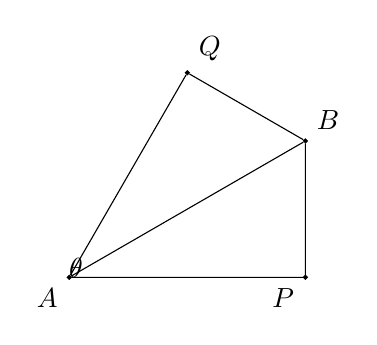
\begin{tikzpicture}
[scale=1,>=stealth,point/.style={draw,circle,fill = black,inner sep=0.5pt},]

\node (A) at (0,0)[point,label=below left:$A$] {};
\node (P) at (3, 0)[point,label=below left:$P$] {};
%\node (Q) at ($({3*\cos{60}}, {3*\sin{60}})$)[point,label=below right:$Q$] {};
%\node (B) at ($({3.4641*\cos{30}}, {3.4641*\sin{30}})$)[point,label=above right:$B$] {};
\node (Q) at (1.5, 2.598)[point,label=above right:$Q$] {};
\node (B) at (3, 1.732)[point,label=above right:$B$] {};




\draw (A) -- node[left] {$\textrm{}$} (P) -- node[below] {$\textrm{}$} (B) -- node[above,xshift=2mm] {$\textrm{}$} (Q);
\draw (A)--(Q);
\draw (A)--(B);


\tkzFillAngle[fill=green!40,size=0.4cm,mark=](P,A,B)
\tkzFillAngle[fill=orange!40,size=0.5cm,mark=](B,A,Q)
\tkzMarkRightAngle[fill=blue,size=.3](A,Q,B);
\tkzMarkRightAngle[fill=purple,size=.3](A,P,B);

%\tkzMarkRightAngle[fill=orange!40,size=0.4cm,mark=](A,Q,B)
%\tkzMarkRightAngle[fill=green!40,size=0.5cm,mark=](A,P,B)

\tkzLabelAngle[pos=0.7](P,A,Q){$\theta$}
%\tkzLabelAngle[pos=0.7](P,A,B){$\gamma$}


\end{tikzpicture}
}
\caption{ }
\label{fig:8.1.26_angle}	
\end{figure}

%\renewcommand{\thefigure}{\theenumi.\arabic{figure}}

\item {Construction: } See Fig. \ref{fig:8.1.26_angle}
The input parameters are
% 
\begin{align}
\vec{A} &= \myvec{0\\0},
\vec{P} &= \myvec{1\\0}
\vec{Q} &= \myvec{\cos \theta \\ \sin \theta}
\end{align}
resulting in 
% 
%
\begin{align}
\vec{B} &= \lambda{\vec{P}+\vec{Q}}
\\
\because \brak{\vec{B} - \vec{P}}^T \vec{P} &= 0,
\\
\brak{\lambda -1}+ \lambda \vec{Q}^T \vec{P} &=0
\end{align}
resulting in 
\begin{align}
\lambda = \frac{1}{1+\vec{P}^T \vec{Q} }
\end{align}



\item 	In Fig. \ref{fig:8.1.26_angle} using ASA congruence,
\begin{align}
\triangle APB &\cong \triangle AQB
\\
\implies BP = BQ
\end{align}

\end{enumerate}

\item $ABCE$ is a quadrilateral and $D$ is a point on $BC$ such that, $AC = AE, AB = AD$ and $\angle  BAD = \angle  EAC$. Show that $BC = DE$.
%
\item In right triangle $ABC$, right angled at $C, M$ is the mid-point of hypotenuse $AB$. $C$ is joined to $M$ and produced to a point $D$ such that $DM = CM$. Point $D$ is joined to point $B$.
Show that: 
\begin{enumerate}
\item $ \triangle  AMC \cong  \triangle  BMD $
\item $\angle  DBC$ is a right angle. 
\item $\triangle  DBC \cong  \triangle  ACB$
\item $ CM = \frac{1}{ 2} AB$
\end{enumerate}
%
See  Fig. \ref{fig:8.1.28}.
%\solution 
\begin{enumerate}
%\renewcommand{\theequation}{\theenumi}
%\begin{enumerate}[label=\thesection.\arabic*.,ref=\thesection.\theenumi]
%\numberwithin{equation}{enumi}
%\item 
\item {\em Construction:} 
%with angles $\phase{ A},\phase{ C}$ and $\phase{ B}$ and sides $a, b$ and $c$.  The unique feature of this triangle is $\phase{ C}$ which is defined to be $90\degree$.%
%\renewcommand{\thefigure}{\theenumi.\arabic{figure}}
From the given information, 
%$\triangle ABC$ are 
\begin{align}
\label{eq:8.1.28_constr_a}
\vec{A} &= \myvec{0\\b} 
\\
 \vec{C} &= \myvec{0\\0}, 
\label{eq:8.1.28_constr_c}
\\
\vec{B} &= \myvec{a\\0}
\label{eq:8.1.28_constr_b}
\end{align}
$\because \vec{M}$ is the midpoint of $AB$,
\begin{align}
\vec{M}= \frac{\vec{A}+\vec{B}}{2} = \frac{1}{2}\myvec{a\\b}
\label{eq:8.1.28_constr_m}
\end{align}
%
Also, $\vec{M}$ is given to be the midpoint of $C$.  Hence, 
\begin{align}
\vec{M}&= \frac{\vec{C}+\vec{D}}{2}
\\
\implies \vec{D} &= 2 \vec{M} - \vec{C} = \myvec{a\\b}
\label{eq:8.1.28_constr_d}
\end{align}
\begin{figure}[!ht]
\centering
\resizebox{\columnwidth}{!}{

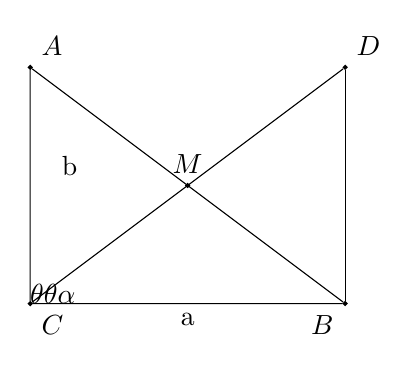
\begin{tikzpicture}
[scale=1,>=stealth,point/.style={draw,circle,fill = black,inner sep=0.5pt},]

%Triangle sides
\def\a{4}
\def\b{3}
\def\c{sqrt(\a^2+\c^2)}



%Labeling points
\node (A) at (0,\b)[point,label=above right:$A$] {};
\node (B) at (\a, 0)[point,label=below left:$B$] {};
\node (C) at (0, 0)[point,label=below right:$C$] {};
\node (M) at (\a*0.5,\b*0.5)[point,label=above:$M$] {};
\node (D) at (\a,\b)[point,label=above right:$D$] {};


%Drawing triangle ABC
\draw (A) -- node[left] {$\textrm{}$} (B) -- node[below] {$\textrm{a}$} (C) -- node[above,xshift=5mm] {$\textrm{b}$} (A);

%Joining CD
\draw (C)--(D);
%Joining BD
\draw (B)--(D);

%Drawing and marking angles
\tkzMarkAngle[fill=orange!40,size=0.5cm,mark=](A,M,C)
\tkzMarkAngle[fill=orange!40,size=0.5cm,mark=](B,M,D)
\tkzMarkAngle[fill=green!40,size=0.5cm,mark=](A,B,C)
\tkzMarkRightAngle[fill=blue!20,size=.2](A,C,B)
\tkzMarkRightAngle[fill=blue!20,size=.2](D,B,C)
\tkzLabelAngle[pos=0.65](A,M,C){$\theta$}
\tkzLabelAngle[pos=0.65](B,M,D){$\theta$}
\tkzLabelAngle[pos=0.65](A,B,C){$\alpha$}


\end{tikzpicture}
}
\caption{}
\label{fig:8.1.28}	
\end{figure}
%
%
%\renewcommand{\thefigure}{\theenumi}
%
%\item List the design parameters for construction
%\label{const:table1}
%\\
%\solution See Table. \ref{table:table1}. 
%%
%\begin{table}[ht!]
%\centering
%%\begin{tabular}{ |p{3cm}|p{3cm}|  }
%%\hline
%% \multicolumn{2}{|c|}{Initial Input Values.} \\
%%\hline
%%a & 4\\
%%\hline
%%b & 3\\
%%\hline
%%$\phase{(ACB)$ & $90^{\circ}$ \\
%%\hline
%%\end{tabular}
%%%%%%%%%%%%%%%%%%%%%%%%%%%%%%%%%%%%%%%%%%%%%%%%%%%%%%%%%%%%%%%%%%%%%%%
%%                                                                  %%
%%  This is the header of a LaTeX2e file exported from Gnumeric.    %%
%%                                                                  %%
%%  This file can be compiled as it stands or included in another   %%
%%  LaTeX document. The table is based on the longtable package so  %%
%%  the longtable options (headers, footers...) can be set in the   %%
%%  preamble section below (see PRAMBLE).                           %%
%%                                                                  %%
%%  To include the file in another, the following two lines must be %%
%%  in the including file:                                          %%
%%        \def\inputGnumericTable{}                                 %%
%%  at the beginning of the file and:                               %%
%%        \input{name-of-this-file.tex}                             %%
%%  where the table is to be placed. Note also that the including   %%
%%  file must use the following packages for the table to be        %%
%%  rendered correctly:                                             %%
%%    \usepackage[latin1]{inputenc}                                 %%
%%    \usepackage{color}                                            %%
%%    \usepackage{array}                                            %%
%%    \usepackage{longtable}                                        %%
%%    \usepackage{calc}                                             %%
%%    \usepackage{multirow}                                         %%
%%    \usepackage{hhline}                                           %%
%%    \usepackage{ifthen}                                           %%
%%  optionally (for landscape tables embedded in another document): %%
%%    \usepackage{lscape}                                           %%
%%                                                                  %%
%%%%%%%%%%%%%%%%%%%%%%%%%%%%%%%%%%%%%%%%%%%%%%%%%%%%%%%%%%%%%%%%%%%%%%



%%  This section checks if we are begin input into another file or  %%
%%  the file will be compiled alone. First use a macro taken from   %%
%%  the TeXbook ex 7.7 (suggestion of Han-Wen Nienhuys).            %%
\def\ifundefined#1{\expandafter\ifx\csname#1\endcsname\relax}


%%  Check for the \def token for inputed files. If it is not        %%
%%  defined, the file will be processed as a standalone and the     %%
%%  preamble will be used.                                          %%
\ifundefined{inputGnumericTable}

%%  We must be able to close or not the document at the end.        %%
	\def\gnumericTableEnd{\end{document}}


%%%%%%%%%%%%%%%%%%%%%%%%%%%%%%%%%%%%%%%%%%%%%%%%%%%%%%%%%%%%%%%%%%%%%%
%%                                                                  %%
%%  This is the PREAMBLE. Change these values to get the right      %%
%%  paper size and other niceties.                                  %%
%%                                                                  %%
%%%%%%%%%%%%%%%%%%%%%%%%%%%%%%%%%%%%%%%%%%%%%%%%%%%%%%%%%%%%%%%%%%%%%%

	\documentclass[12pt%
			  %,landscape%
                    ]{report}
       \usepackage[latin1]{inputenc}
       \usepackage{fullpage}
       \usepackage{color}
       \usepackage{array}
       \usepackage{longtable}
       \usepackage{calc}
       \usepackage{multirow}
       \usepackage{hhline}
       \usepackage{ifthen}

	\begin{document}


%%  End of the preamble for the standalone. The next section is for %%
%%  documents which are included into other LaTeX2e files.          %%
\else

%%  We are not a stand alone document. For a regular table, we will %%
%%  have no preamble and only define the closing to mean nothing.   %%
    \def\gnumericTableEnd{}

%%  If we want landscape mode in an embedded document, comment out  %%
%%  the line above and uncomment the two below. The table will      %%
%%  begin on a new page and run in landscape mode.                  %%
%       \def\gnumericTableEnd{\end{landscape}}
%       \begin{landscape}


%%  End of the else clause for this file being \input.              %%
\fi

%%%%%%%%%%%%%%%%%%%%%%%%%%%%%%%%%%%%%%%%%%%%%%%%%%%%%%%%%%%%%%%%%%%%%%
%%                                                                  %%
%%  The rest is the gnumeric table, except for the closing          %%
%%  statement. Changes below will alter the table's appearance.     %%
%%                                                                  %%
%%%%%%%%%%%%%%%%%%%%%%%%%%%%%%%%%%%%%%%%%%%%%%%%%%%%%%%%%%%%%%%%%%%%%%

\providecommand{\gnumericmathit}[1]{#1} 
%%  Uncomment the next line if you would like your numbers to be in %%
%%  italics if they are italizised in the gnumeric table.           %%
%\renewcommand{\gnumericmathit}[1]{\mathit{#1}}
\providecommand{\gnumericPB}[1]%
{\let\gnumericTemp=\\#1\let\\=\gnumericTemp\hspace{0pt}}
 \ifundefined{gnumericTableWidthDefined}
        \newlength{\gnumericTableWidth}
        \newlength{\gnumericTableWidthComplete}
        \newlength{\gnumericMultiRowLength}
        \global\def\gnumericTableWidthDefined{}
 \fi
%% The following setting protects this code from babel shorthands.  %%
 \ifthenelse{\isundefined{\languageshorthands}}{}{\languageshorthands{english}}
%%  The default table format retains the relative column widths of  %%
%%  gnumeric. They can easily be changed to c, r or l. In that case %%
%%  you may want to comment out the next line and uncomment the one %%
%%  thereafter                                                      %%
\providecommand\gnumbox{\makebox[0pt]}
%%\providecommand\gnumbox[1][]{\makebox}

%% to adjust positions in multirow situations                       %%
\setlength{\bigstrutjot}{\jot}
\setlength{\extrarowheight}{\doublerulesep}

%%  The \setlongtables command keeps column widths the same across  %%
%%  pages. Simply comment out next line for varying column widths.  %%
\setlongtables

\setlength\gnumericTableWidth{%
	53pt+%
	53pt+%
0pt}
\def\gumericNumCols{2}
\setlength\gnumericTableWidthComplete{\gnumericTableWidth+%
         \tabcolsep*\gumericNumCols*2+\arrayrulewidth*\gumericNumCols}
\ifthenelse{\lengthtest{\gnumericTableWidthComplete > \linewidth}}%
         {\def\gnumericScale{\ratio{\linewidth-%
                        \tabcolsep*\gumericNumCols*2-%
                        \arrayrulewidth*\gumericNumCols}%
{\gnumericTableWidth}}}%
{\def\gnumericScale{1}}

%%%%%%%%%%%%%%%%%%%%%%%%%%%%%%%%%%%%%%%%%%%%%%%%%%%%%%%%%%%%%%%%%%%%%%
%%                                                                  %%
%% The following are the widths of the various columns. We are      %%
%% defining them here because then they are easier to change.       %%
%% Depending on the cell formats we may use them more than once.    %%
%%                                                                  %%
%%%%%%%%%%%%%%%%%%%%%%%%%%%%%%%%%%%%%%%%%%%%%%%%%%%%%%%%%%%%%%%%%%%%%%

\ifthenelse{\isundefined{\gnumericColA}}{\newlength{\gnumericColA}}{}\settowidth{\gnumericColA}{\begin{tabular}{@{}p{53pt*\gnumericScale}@{}}x\end{tabular}}
\ifthenelse{\isundefined{\gnumericColB}}{\newlength{\gnumericColB}}{}\settowidth{\gnumericColB}{\begin{tabular}{@{}p{53pt*\gnumericScale}@{}}x\end{tabular}}

\begin{tabular}[c]{%
	b{\gnumericColA}%
	b{\gnumericColB}%
	}

%%%%%%%%%%%%%%%%%%%%%%%%%%%%%%%%%%%%%%%%%%%%%%%%%%%%%%%%%%%%%%%%%%%%%%
%%  The longtable options. (Caption, headers... see Goosens, p.124) %%
%	\caption{The Table Caption.}             \\	%
% \hline	% Across the top of the table.
%%  The rest of these options are table rows which are placed on    %%
%%  the first, last or every page. Use \multicolumn if you want.    %%

%%  Header for the first page.                                      %%
%	\multicolumn{2}{c}{The First Header} \\ \hline 
%	\multicolumn{1}{c}{colTag}	%Column 1
%	&\multicolumn{1}{c}{colTag}	\\ \hline %Last column
%	\endfirsthead

%%  The running header definition.                                  %%
%	\hline
%	\multicolumn{2}{l}{\ldots\small\slshape continued} \\ \hline
%	\multicolumn{1}{c}{colTag}	%Column 1
%	&\multicolumn{1}{c}{colTag}	\\ \hline %Last column
%	\endhead

%%  The running footer definition.                                  %%
%	\hline
%	\multicolumn{2}{r}{\small\slshape continued\ldots} \\
%	\endfoot

%%  The ending footer definition.                                   %%
%	\multicolumn{2}{c}{That's all folks} \\ \hline 
%	\endlastfoot
%%%%%%%%%%%%%%%%%%%%%%%%%%%%%%%%%%%%%%%%%%%%%%%%%%%%%%%%%%%%%%%%%%%%%%

\hhline{|-|-}
	 \multicolumn{1}{|p{\gnumericColA}|}%
	{\gnumericPB{\centering}\gnumbox{Parameter}}
	&\multicolumn{1}{p{\gnumericColB}|}%
	{\gnumericPB{\centering}\gnumbox{Value}}
\\
\hhline{|--|}
	 \multicolumn{1}{|p{\gnumericColA}|}%
	{\gnumericPB{\centering}\gnumbox{a}}
	&\multicolumn{1}{p{\gnumericColB}|}%
	{\gnumericPB{\centering}\gnumbox{5}}
\\
\hhline{|--|}
	 \multicolumn{1}{|p{\gnumericColA}|}%
	{\gnumericPB{\centering}\gnumbox{b}}
	&\multicolumn{1}{p{\gnumericColB}|}%
	{\gnumericPB{\centering}\gnumbox{6}}
\\
\hhline{|--|}
	 \multicolumn{1}{|p{\gnumericColA}|}%
	{\gnumericPB{\centering}\gnumbox{c}}
	&\multicolumn{1}{p{\gnumericColB}|}%
	{\gnumericPB{\centering}\gnumbox{4}}
\\
\hhline{|--|}
	 \multicolumn{1}{|p{\gnumericColA}|}%
	{\gnumericPB{\centering}\gnumbox{d}}
	&\multicolumn{1}{p{\gnumericColB}|}%
	{\gnumericPB{\centering}\gnumbox{4}}
\\
\hhline{|-|-|}
\end{tabular}

\ifthenelse{\isundefined{\languageshorthands}}{}{\languageshorthands{\languagename}}
\gnumericTableEnd

%\caption{To construct $\triangle ACB$}
%\label{table:table1}	
%\end{table}
%\item
%	For simplicity, let the greek letter $\alpha = \phase{ B$.  We have the following definitions.
%\begin{equation}
%\label{eq:8.1.28_tri_trig_defs}
%\begin{matrix}
	%\sin \theta = \frac{b}{c} & 	\cos \theta = \frac{a}{c} \\
	%\tan \theta = \frac{c}{a} & \cot \theta = \frac{1}{\tan \theta} \\
	%\csc \theta = \frac{1}{\sin \theta} & \sec \theta = \frac{1}{\cos \theta}
	%\end{equation}
%
%\item Find the coordinates of the various points in Fig. \ref{fig:tri_right_angle}
%\label{const:tri_right_angle}
%\\
%
%\solution 
%
%The values are listed in 
%%\item List the  derived values.
%%\label{const:table2}
%%\\
%%\solution See  
%Table. \ref{table:table2} 
%\begin{table}[ht!]
%%\centering
%%\begin{tabular}{ |p{3cm}|p{3cm}|  }
%%\hline
%% \multicolumn{2}{|c|}{Derived Values.} \\
%%\hline
%%$\vec{M}$ & $$\begin{pmatrix}2\\1.5\end{pmatrix}$$\\						
%%\hline
%%$\vec{D}$ & $$\begin{pmatrix}4\\3\end{pmatrix} $$\\
%%\hline
%\input{./tables/inp1.tex}
%\caption{To construct $\triangle DBC$}
%\label{table:table2}
%
%\end{table}
%
%\item Draw Fig. \ref{fig:tri_right_angle}.	
%\\
%\solution The  following Python code generates Fig. \ref{fig:tri_sss_py}
%%
%\begin{lstlisting}
%codes/triangle.py
%\end{lstlisting}
%\begin{figure}[!ht]
%\centering
%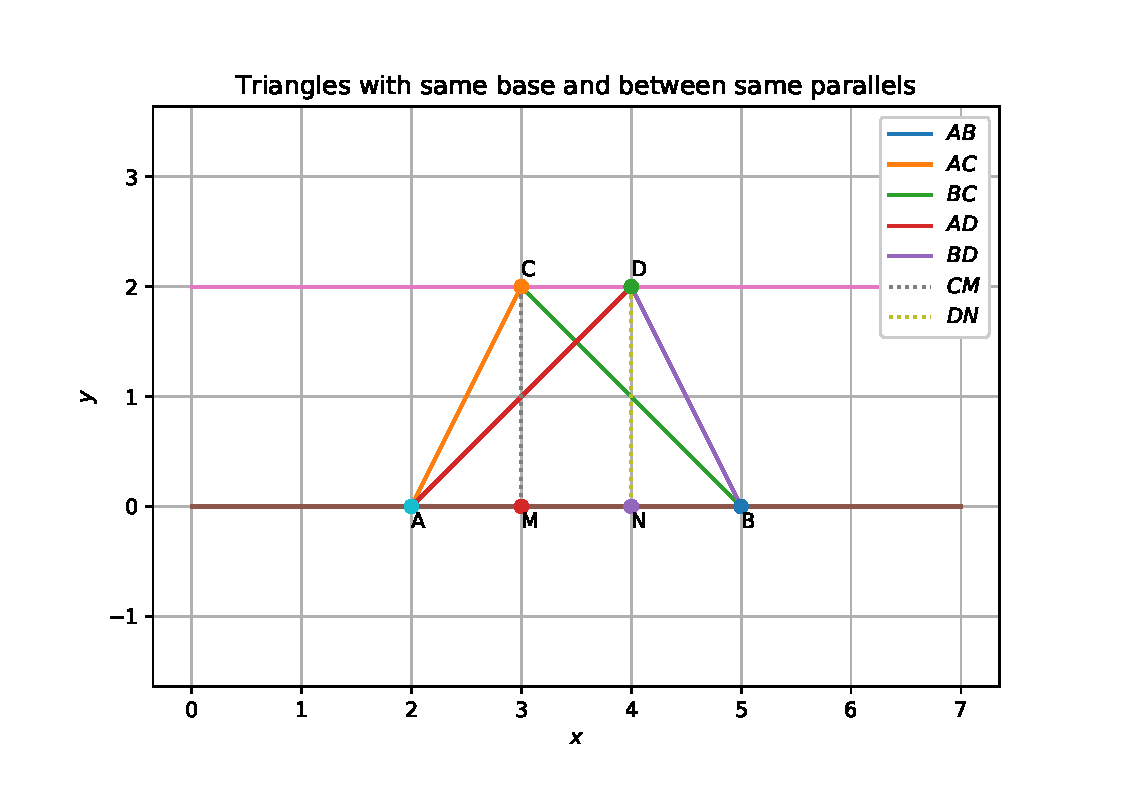
\includegraphics[width=\columnwidth]{./figs/triangle.eps}
%\caption{Triangle generated using python}
%\label{fig:tri_sss_py}
%\end{figure}
%
%%
%and the equivalent latex-tikz code generating Fig. \ref{fig:tri_right_angle} is 
%\begin{lstlisting}
%figs/triangle.tex
%\end{lstlisting}
%
%The above latex code can be compiled as a standalone document as
%\begin{lstlisting}
%figs/triangle_fig.tex
%\end{lstlisting}

%

%

%
%

%\end{enumerate}

%\renewcommand{\theequation}{\theenumi}
%\begin{enumerate}[label=\thesection.\arabic*.,ref=\thesection.\theenumi]
%\numberwithin{equation}{enumi}
	
\item {\em Proof: }
%\solution
From Fig. \ref{fig:8.1.28},	
%$\triangle AMC \cong \triangle DMB$  by SAS congruency $\because$
%\begin{enumerate}
%\item $AM = BM$
%\item $CM = DM$
%\item $\phase{AMC}$ = $\phase{DMB}$ ( Vertically Opposite Angles)
%\end{enumerate}
%
%\begin{figure}[!ht]
%\centering
%\resizebox{\columnwidth}{!}{

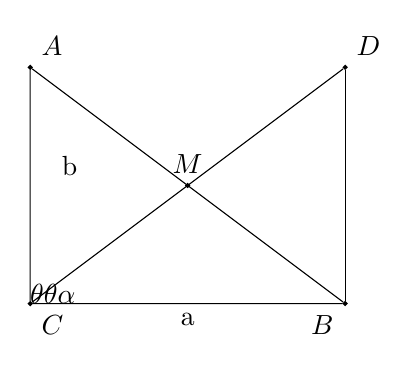
\begin{tikzpicture}
[scale=1,>=stealth,point/.style={draw,circle,fill = black,inner sep=0.5pt},]

%Triangle sides
\def\a{4}
\def\b{3}
\def\c{sqrt(\a^2+\c^2)}



%Labeling points
\node (A) at (0,\b)[point,label=above right:$A$] {};
\node (B) at (\a, 0)[point,label=below left:$B$] {};
\node (C) at (0, 0)[point,label=below right:$C$] {};
\node (M) at (\a*0.5,\b*0.5)[point,label=above:$M$] {};
\node (D) at (\a,\b)[point,label=above right:$D$] {};


%Drawing triangle ABC
\draw (A) -- node[left] {$\textrm{}$} (B) -- node[below] {$\textrm{a}$} (C) -- node[above,xshift=5mm] {$\textrm{b}$} (A);

%Joining CD
\draw (C)--(D);
%Joining BD
\draw (B)--(D);

%Drawing and marking angles
\tkzMarkAngle[fill=orange!40,size=0.5cm,mark=](A,M,C)
\tkzMarkAngle[fill=orange!40,size=0.5cm,mark=](B,M,D)
\tkzMarkAngle[fill=green!40,size=0.5cm,mark=](A,B,C)
\tkzMarkRightAngle[fill=blue!20,size=.2](A,C,B)
\tkzMarkRightAngle[fill=blue!20,size=.2](D,B,C)
\tkzLabelAngle[pos=0.65](A,M,C){$\theta$}
\tkzLabelAngle[pos=0.65](B,M,D){$\theta$}
\tkzLabelAngle[pos=0.65](A,B,C){$\alpha$}


\end{tikzpicture}
}
%\caption{}
%\label{fig:8.1.28}	
%\end{figure}
%\item From \eqref{eq:constr_b}, \eqref{eq:constr_c} and \eqref{eq:constr_d},
%%
%%
\begin{align}
\brak{\vec{D}-\vec{B}}^T
\brak{\vec{B}-\vec{C}} &= \myvec{0 & b}\myvec{a \\ 0} = 0
\\
\implies BD \perp BC
\end{align}
%%
%\item From \eqref{eq:constr_a}, \eqref{eq:constr_b}, \eqref{eq:constr_c} and \eqref{eq:constr_d},
\begin{align}
\norm{\vec{A}-\vec{B}} &= \norm{\myvec{-a \\ b}}
\\
\norm{\vec{C}-\vec{D}} &= \norm{\myvec{-a \\ -b}}
\\
\implies \norm{\vec{A}-\vec{B}} &= \norm{\vec{C}-\vec{D}}\\
\text{or, } AB &=CD
\label{eq:solution_abcd}
\end{align}
%%
Noting that BC is the common side, from RHS congruence,  $\triangle ACB \cong  \triangle DCB$.
\subitem  From \eqref{eq:solution_abcd}, noting that $\vec{M}$ is the mid point of both $AB$ and $CD$, 
\begin{align}
CM = \frac{1}{2}CD =\frac{1}{2} AB
\end{align}



%\end{enumerate}

\end{enumerate}

\item In an isosceles $\triangle ABC$, with $AB = AC$, the bisectors of $\angle B$ and $\angle C$ intersect each other at $O$. Join $A$ to $O$. Show that :
\begin{enumerate} 
\item $OB = OC$ 
\item $AO$ bisects $\angle A$
\end{enumerate}
\item In $\triangle ABC$, $AD$ is the perpendicular bisector of $BC$. Show that $\triangle ABC$ is an isosceles triangle in which $AB = AC$.
\item $ABC$ is an isosceles triangle in which altitudes $BE$ and $CF$ are drawn to equal sides $AC$ and $AB$ respectively . Show that these altitudes are equal.
%
\item $ABC$ is a triangle in which altitudes $BE$ and $CF$ to sides $AC$ and $AB$ are equal. Show that
%
\begin{enumerate} 
\item $\triangle  ABE \cong  \triangle  ACF $
\item  $AB = AC$, i.e., $ABC$ is an isosceles triangle.
\end{enumerate}
%
\item $ABC$ and $DBC$ are two isosceles triangles on the same base $BC$. Show that $\angle ABD = \angle ACD$.
%
\item  $\triangle  ABC$ and $\triangle  DBC$ are two isosceles triangles on the same base $BC$ and vertices $A$ and $D$ are on the same side of $BC$. If $AD$ is extended to intersect $BC$ at $P$, show that
\begin{enumerate}
\item $\triangle  ABD \cong  \triangle  ACD $
\item $\triangle  ABP \cong  \triangle  ACP $
\item $AP$ bisects $\angle  A$ as well as $\angle  D$. 
\item $AP$ is the perpendicular bisector of $BC$.
\end{enumerate}
\item $AD$ is an altitude of an isosceles $\triangle ABC$ in which $AB = AC$. Show that 
\begin{enumerate}
\item $AD$ bisects $BC$
\item $AD$ bisects $\angle  A$. 
\end{enumerate}

\item  Two sides $AB$ and $BC$ and median $AM$ of one triangle $ABC$ are respectively equal to sides $PQ$ and $QR$ and median $PN$ of $\triangle  PQR$. Show that: 
\begin{enumerate}
\item $\triangle  ABM \cong  \triangle  PQN $
\item $\triangle  ABC \cong  \triangle  PQR$
\end{enumerate}
\begin{enumerate}

%\renewcommand{\thefigure}{\theenumi.\arabic{figure}}
\begin{figure}[!ht]
\centering
\resizebox{\columnwidth}{!}{%\documentclass{article}
%\usepackage[utf8]{inputenc}
%\usepackage{tikz}
%\usepackage{tkz-euclide}
%\begin{document}

\begin{tikzpicture}
[scale=1,>=stealth,point/.style={draw,circle,fill = black,inner sep=0.5pt},]

%Triangle ABC
\def\a{6}
\def\b{4}
\def\c{5}
 
%Coordinates of A
%\def\p{(\a^2 + \c^2 - \b^2)/ (2*\a)}
\def\p{45/12}
\def\q{{sqrt(\c^2-\p^2)}}

%Labeling points
\node (A) at (\p,\q)[point,label=above right:$A$] {};
\node (B) at (0, 0)[point,label=below left:$B$] {};
\node (C) at (\a, 0)[point,label=below right:$C$] {};

%Foot median AM

\node (M) at (\a/2,0)[point,label=above right:$M$] {};

%Drawing triangle ABC
\draw (A) -- node[left] {$\textrm{c}$} (B) -- node[below] {$\textrm{a}$} (C) -- node[above,xshift=2mm] {$\textrm{b}$} (A);

%Drawing median AM
\draw (A) -- node[left] {$\textrm{}$}(M);

%Drawing and marking angles
\tkzMarkAngle[fill=orange!40,size=0.5cm,mark=](C,B,A)
\tkzLabelAngle[pos=-0.9](A,B,C){$\alpha$}

\end{tikzpicture}

\begin{tikzpicture}
[scale=1,>=stealth,point/.style={draw,circle,fill = black,inner sep=0.5pt},]

%Triangle PQR
\def\p{6}
\def\q{4}
\def\r{5}
 
%Coordinates of P
%\def\x{(\p^2 + \r^2 - \q^2)/ (2*\p)}
\def\x{45/12}
\def\z{{sqrt(\r^2-\x^2)}}

%Labeling points
\node (P) at (\x,\z)[point,label=above right:$P$] {};
\node (Q) at (0, 0)[point,label=below left:$Q$] {};
\node (R) at (\p, 0)[point,label=below right:$R$] {};

%Foot of median

\node (N) at (\p/2,0)[point,label=above right:$N$] {};

%Drawing triangle PQR
\draw (P) -- node[left] {$\textrm{r}$} (Q) -- node[below] {$\textrm{p}$} (R) -- node[above,xshift=2mm] {$\textrm{q}$} (P);

%Drawing median PN
\draw (P) -- node[left] {$\textrm{}$}(N);

%Drawing and marking angles
\tkzMarkAngle[fill=orange!40,size=0.5cm,mark=](R,Q,P)
\tkzLabelAngle[pos=-0.9](P,Q,R){$\theta$}

\end{tikzpicture}
%\end{document}
}
\caption{$\triangle ABC$ and $\triangle PQR$ by Latex-Tikz}
\label{fig:8.1.36_triangle_latex}	
\end{figure}
%
%
%\renewcommand{\thefigure}{\theenumi}
%

\item {\em Construction: }The coordinates of the various points of triangle ABC in Fig. \ref{fig:8.1.36_triangle_latex} are
%\label{}
%
\begin{align}
\vec{B} &= \myvec{0\\0} ,
\label{eq:8.1.36_constr_b}
\\
 \vec{C} &= \myvec{a\\0}, 
\label{eq:8.1.36_constr_c}
\end{align}

$\because \vec{M}$ is the midpoint of $BC$,
\begin{align}
\vec{M}= \frac{\vec{B}+\vec{C}}{2} =\myvec{a/2\\0},
\label{eq:8.1.36_constr_m}
\end{align}
%
$\triangle PQR$ is a horizontal translation of $\triangle ABC$.  Hence, if 
\begin{align}
\vec{Q}= \myvec{q\\0},
\label{eq:8.1.36_constr_q}
\end{align}
\begin{align}
\vec{P}= \vec{A} + \vec{Q}
\\
\vec{R}= \vec{C} + \vec{Q}
\end{align}

%




%\noindent a) \\
    In $\triangle ABM$  and  $\triangle PQN$ \newline 
    AB = PQ (Given)  \newline
    AM = PN (Given) \newline
    Since M and N are midpoints and BC = QR , \newline
    BM = QR  \newline
    :. By SSS congruence rule , $\triangle ABM \cong \triangle PQN$  \newline
    
        This implies that $\angle ABM = \angle PQN$ i.e $\alpha = \theta$
    \newline
    \\
    \\
b) \\   
Now in $\triangle ABC$  and  $\triangle PQR$ \newline 
AB = PQ (Given)  \newline
$\alpha = \theta$ \newline
BC = QR (Given)\newline
:. By SAS congruence rule , $\triangle ABC \cong \triangle PQR$ 
    



\end{enumerate}

\item  $BE$ and $CF$ are two equal altitudes of a triangle $ABC$. Using RHS congruence rule, prove that the triangle $ABC$ is isosceles.
\item  $ABC$ is an isosceles triangle with $AB = AC$. Draw $AP \perp BC$ to show that $\angle  B = \angle  C$.
%
\item $\triangle ABC$ is an isosceles triangle in which $AB = AC$. Side $BA$ is produced to $D$ such that $AD = AB$. Show that $\angle BCD$ is a right angle.
%
\item $ABC$ is a right angled triangle in which $\angle A$ = 90$\degree$ and $AB = AC$. Find $\angle B$ and $\angle C$.
%
\item Show that in a right angled triangle, the hypotenuse is the longest side.
\item Sides AB and AC of $\triangle  ABC$ are extended to points P and Q respectively. Also, $\angle  PBC < \angle  QCB$. Show that $AC > AB$.

\item Line segments $AD$ and $BC$ intersect at $O$ and form $\triangle OAB$ and $\triangle ODC$. $\angle  B < \angle  A$ and $\angle  C < \angle  D$. Show that $AD < BC$.

\item $AB$ and $CD$ are respectively the smallest and longest sides of a quadrilateral $ABCD$. Show that $\angle  A > \angle  C$ and $\angle  B > \angle  D$.
%
\item In $\triangle PQR,  PR > PQ$ and $PS$ bisects $\angle  QPR$. Prove that $\angle  PSR > \angle  PSQ$.
%
\begin{enumerate}

\begin{figure}[!ht]
\centering
\resizebox{\columnwidth}{!}{\begin{tikzpicture}[scale = 1.5,>=stealth,point/.style={draw,circle,fill=black, inner sep=0.5pt},]

\node (Q) at (0, 0)[point,label=below left:$Q$] {};
\node (R) at (6, 0)[point,label=below right:$R$] {};
\node (P) at (2.25, 3.307189138830738)[point,label=above right:$P$] {};
\node (S) at (8/3, 0)[point,label=below:$S$] {};
\node (G) at (4/3, 0)[label=below:$y$] {};

\draw (P) -- node[below=5pt]{}(Q) -- (R) -- (P) -- (S);

\tkzMarkAngle[fill=green!20, mark=|](Q,P,S)
\tkzMarkAngle[fill=green!20, mark=|](S,P,R)

\end{tikzpicture}}
\caption{}
\label{fig:8.1.45_triangle1}	
\end{figure}

\item {\em Construction: } See Fig. \ref{fig:8.1.45_triangle1}.  The input parameters are
\begin{align}
\vec{P} &= \myvec{p\\q},
%\label{eq:constr_a} 
 \vec{Q} &= \myvec{0\\0}, 
\label{eq:constr_b}
\\
\vec{R} &= \myvec{a\\0},
%\label{eq:constr_c}
\label{eq:constr_d}
\end{align}
%
where $\vec{P}$  is obtained by choosing $PR > PQ$.
$\because PS$ is the angle bisector, its equation is given by (see Problem \ref{prob:8.1.23})
%
\begin{align}
PS: \vec{x} = \vec{P} + \lambda\brak{\frac{\vec{P}-\vec{Q}}{\norm{\vec{P}-\vec{Q}}}+\frac{\vec{P}-\vec{R}}{\norm{\vec{P}-\vec{R}}}}
\end{align}
%
$\vec{S}$ is obtained as the intersection of $PS$ and $QR$.



\item {\em Proof: } From the given information,
\begin{align}
\phase{Q} &> \phase{R}
\\
\implies \phase{Q} + \phase{SPQ}&> \phase{R}+  \phase{SPR} 
\\
\implies  \phase{PSQ}&>   \phase{PSR} 
\end{align}
$\because PS$ is the angle bisector.

\end{enumerate}

\item Show that of all line segments drawn from a given point not on it, the perpendicular line segment is the shortest.
%
\item $ABCD$ is a trapezium with $AB  \parallel  DC$. $E$ and $F$ are points on non-parallel sides $AD$ and $BC$ respectively such that $EF$ is parallel to $AB$
. Show that
$\frac{AE}{ED}=\frac{ BF}{  FC}$ .
\begin{enumerate}
\begin{figure}[!ht]
\centering
\resizebox{\columnwidth}{!}{%Exercise 8.1 prob 47
\begin{tikzpicture}
[scale=0.5,>=stealth,point/.style={draw,circle,fill = black,inner sep=0.5pt},]
%\tikzset{shift={(-3,0)}}
%Triangle sides
\def\a{4}
\def\c{9}
\def\xA{4}
\def\h{3}
\def\k{1}
%\def\c{7.5}
\def\yE{\h/2}
%Labeling points
\node (D) at (0,0)[point,label=below left:$D$] {};
\node (B) at ({\xA+\a}, \h )[point,label=above right:$B$] {};
\node (C) at (\c, 0)[point,label=below right:$C$] {};
%\node (E) at (2, \yE)
%\node (F) at (8.5, \yE)[point,label=below right:$F$] {};
%\node (M) at (\xA,\yE)[point,label=above right:$M$] {};
%\node (N) at ({\xA+\a}, \yE)[point,label=above left:$N$] {};
%\node (X) at (\xA , 0)[point,label=below left:$X$] {};
%\node (Y) at ({\xA+\a}, 0)[point,label=below right:$Y$] {};
\node (A) at (\xA , \h)[point,label=above left:$A$] {};
\node (E) at ($(D)!0.5!(A)$)[point,label=above left:$E$] {};
\node (F) at ($(B)!0.5!(C)$)[point,label=above right:$F$] {};



%A



%Drawing parallelogram ABCD
\draw (A) -- (B)--(C) --(D)--(A);
%\draw (A) --(X);
\draw (E) --(F);
\draw(A)--node[right]{$\textrm{k}$} (E)--node[right]{$\textrm{1}$} (D);
\draw(B)--node[left]{$\textrm{m}$} (F)--node[left]{$\textrm{1}$} (C);


%\draw (B) --(Y);
%marking right angles
%\tkzMarkRightAngle[fill=green!20,size=.2](D,X,A)
%\tkzMarkRightAngle[fill=green!20,size=.2](C,Y,B)


%
\end{tikzpicture}
}
\caption{}
\label{fig:8.1.47_trapezium_ABCD}	
\end{figure}

\item {\em Construction: }See Fig. \ref{fig:8.1.47_trapezium_ABCD}.
The input parameters are
\begin{align}
\label{eq:8.1.47_constr_d}
\vec{D} &= \myvec{0\\0} 
\\
\vec{C} &= \myvec{c\\0} 
\\
\vec{A} &= \myvec{p\\q} 
\\
\vec{B} &= \myvec{b\\q}, \quad b < c 
\label{eq:8.1.47_constr_c}
\end{align}
%
For $0 < k < 1$, 
\begin{align}
\label{eq:8.1.47_constr_e}
\vec{E} &= \frac{{k\vec{D} +\vec{A}}}{k+1}
\\
\vec{F} &= \frac{{k\vec{C} +\vec{B}}}{k+1}
\label{eq:8.1.47_constr_f}
\end{align}


\item {\em Proof: }Let 
\begin{align}
\vec{F} &= \frac{{{m\vec{C}} +\vec{B}}}{m+1}
\end{align}
%
From \eqref{eq:8.1.47_constr_e}
\begin{align}
\vec{E} &= \frac{{{k\vec{D}} +\vec{A}}}{k+1}
\\
\implies \vec{E} - \vec{F} &= \frac{{{k\vec{D}} +\vec{A}}}{k+1}-\frac{{{m\vec{C}} +\vec{B}}}{m+1}
\label{eq:8.1.47_sol_EF}
\\
& = \frac{\vec{A}}{k+1}-\frac{{{m\vec{C}} +\vec{B}}}{m+1}
\label{eq:8.1.47_sol_EF2}
\end{align}
$\because D = \vec{0}$.
\begin{align}
\because AB &\parallel BC, 
\\
\vec{C}-\vec{D} &= l\brak{\vec{B}-\vec{A}}
\\
\implies \vec{C} &= l\brak{\vec{B}-\vec{A}}
\label{eq:8.1.47_sol_C}
\end{align}
%
Substituting \eqref{eq:8.1.47_sol_C} in \eqref{eq:8.1.47_sol_EF2},
\begin{align}
 \vec{E} - \vec{F} &= \frac{\vec{A}}{k+1}-\frac{{{ml\brak{\vec{B}-\vec{A}}} +\vec{B}}}{m+1}
\\
 &= \vec{A}\brak{\frac{1}{k+1} + \frac{lm}{m+1}} - \vec{B}\brak{\frac{ml+1}{m+1}}
\label{eq:8.1.47_sol_EFinAB}
\end{align}
But $ EF \parallel AB$. So, for some w
\begin{align}
\implies \vec{E} - \vec{F} = w\brak{\vec{A}-\vec{B}}
\label{eq:8.1.47_sol_EFinAB2}
\end{align}
%
Comparing \eqref{eq:8.1.47_sol_EFinAB2} and \eqref{eq:8.1.47_sol_EFinAB}. We have
\begin{align}
\frac{1}{k+1} + \frac{lm}{m+1} &= \frac{ml+1}{m+1} = w
\\
\implies m+1+\brak{k+1}lm &= \brak{lm+1}\brak{k+1} 
\label{eq:8.1.47_sol_sol}
\\
\text{or, } m &=k
\end{align}

\end{enumerate}

\item $ST$ is a line joining two points on $PQ$ and $PR$ in $\triangle PQR$.  If $\frac{PS}{ SQ}=\frac{PT}{ TR}$ and $ \angle  PST = \angle  PRQ$, prove that $PQR$ is an isosceles triangle.
%
\item If $LM  \parallel  CB$ and $LN  \parallel  CD$, prove that $\frac{AM}{AB} = \frac{ AN}{AD}$.
%
\item $D$ is a point on $AB$ and $E, F$ are points on $BC$ such that $DE  \parallel  AC$ and $DF  \parallel  AE$. Prove that $\frac{BF} {FE} =\frac{BE}  {EC}$.
%
\item $O$ is a point in the interior of $\triangle ABC$. $D$ is a point on $OA$.  If $DE  \parallel  OB$ and $DF  \parallel  OC$. Show that $EF  \parallel  BC$.
\begin{enumerate}
\begin{figure}[!ht]
\centering
\resizebox{\columnwidth}{!}{\begin{tikzpicture}
[scale=2,>=stealth,point/.style={draw,circle,fill = black,inner sep=0.5pt},]

%Triangle sides
\def\a{5}
\def\b{6}
\def\c{4}
 
%Coordinates of A
\def\p{0.5}
\def\q{{sqrt(\c^2-\p^2)}}

%Labeling points
\node (A) at (\p,\q)[point,label=above right:$A$] {};
\node (B) at (0, 0)[point,label=below left:$B$] {};
\node (C) at (\a, 0)[point,label=below right:$C$] {};
\node (O) at (2,1.5)[point,label=below:$O$]{};
%Foot of median

\node (D) at ($(A)!0.5!(O)$)[point,label=below:$D$] {};
\node (E) at ($(A)!0.5!(B)$)[point,label=left:$E$] {};
\node (F) at ($(C)!0.5!(A)$)[point,label=right:$F$] {};

%Drawing triangle ABC
\draw (A) -- node[left, xshift=-5mm,yshift=5mm] {$\textrm{c}$} (B) -- node[below, yshift=-5mm] {$\textrm{a}$} (C) -- node[above right,xshift=2mm,yshift=5mm] {$\textrm{b}$} (A);
\draw (A) -- (D) -- (O);
%Drawing medians BE and CF
\draw (D) -- (E);
\draw (D) -- (F);
\draw (O) -- (B);
\draw (O) -- (C);
%Drawing EF
\draw (E) -- (F);

%Labeling sides
%\node [right] at ($(A)!0.5!(E)$) {$\frac{b}{2}$};
%\node [right] at ($(C)!0.5!(E)$) {$\frac{b}{2}$};
%\node [left] at ($(B)!0.5!(F)$) {$\frac{c}{2}$};
%\node [left] at ($(A)!0.5!(F)$) {$\frac{c}{2}$};




%Angles
\tkzMarkAngle[size=.3](D,E,A)
\tkzMarkAngle[size=.3](O,B,A)
%
\tkzMarkAngle[size=.7](A,F,D)
\tkzMarkAngle[size=.7](A,C,O)
%%
\tkzMarkAngle[size=.2](A,D,E)
\tkzMarkAngle[size=.2](A,O,B)
%%
\tkzMarkAngle[size=.2](F,D,A)
\tkzMarkAngle[size=.2](C,O,A)
%
%\tkzMarkAngle[size=.3](E,A,D)
%\tkzMarkAngle[size=.3](D,A,F)

\begin{comment}
%Angles
\tkzMarkAngle[fill=green!60,size=.3](D,E,A)
\tkzMarkAngle[fill=green!60,size=.3](O,B,A)
%
\tkzMarkAngle[fill=red!60,size=.5](A,F,D)
\tkzMarkAngle[fill=red!60,size=.5](A,C,O)
%%
\tkzMarkAngle[fill=yellow!60,size=.2](A,D,E)
\tkzMarkAngle[fill=yellow!60,size=.2](A,O,B)
%%
\tkzMarkAngle[fill=orange!60,size=.2](F,D,A)
\tkzMarkAngle[fill=orange!60,size=.2](C,O,A)
%
\tkzMarkAngle[fill=blue!60,size=.3](E,A,D)
\tkzMarkAngle[fill=blue!60,size=.3](D,A,F)
\end{comment}
\end{tikzpicture}
}
\caption{}
\label{fig:8.1.51_similar}	
\end{figure}
\item {\em Construction: }
See Fig. \ref{fig:8.1.51_similar}. The input values are
\begin{align}
     \vec{B}= \myvec{0\\0}
    \vec{C}=\myvec{a\\0}
    \vec{A}=\myvec{p\\q}
\end{align}

\subitem The point inside $\triangle ABC$ is generated as
\begin{align}
\vec{O} &= \lambda_1 \brak{\vec{B}-\vec{A}} +  \lambda_2 \brak{\vec{B}-\vec{C}}
\\
0 &< \lambda_1  < 1,
\\
0 &< \lambda_2  < 1,
\\
0 &< \lambda_1+\lambda_2  < 1,
\end{align}
%
by choosing appropriate values of $\lambda_1, \lambda_2$.
\subitem Determination of points D,E and F.
\begin{align}
\vec{D} = \frac{k\vec{A} + \vec{O}}{k+1}, \quad 0 < k < 1
\end{align}
%
where $k$ is an input parameter.
\begin{align}
\because DE &\parallel OB, DF \parallel OC,
\\
\begin{split}
\vec{E} &= \frac{k\vec{A} + \vec{B}}{k+1}, 
\\
\vec{F} &= \frac{k\vec{A} + \vec{C}}{k+1}, 
\end{split}
\label{eq:8.1.51_ef}
\end{align}

\item {\em Proof: }
From \eqref{eq:8.1.51_ef}
\begin{align}
\vec{E} - \vec{F} &= \frac{\vec{B}-\vec{C}}{k+1}, 
\\
\implies EF &\parallel BC
\end{align}


\end{enumerate}

\item $O$ is a point in the interior of $\triangle PQR$.  $A, B and C$ are points on $OP, OQ$ and $OR$ respectively such that $AB  \parallel  PQ$ and $AC  \parallel  PR$. Show that $BC  \parallel  QR$.
%
\item $ABCD$ is a trapezium in which $AB  \parallel  DC$ and its diagonals intersect each other at the point $O$. Show
that
$\frac{AO}{ BO}=\frac{CO}{  DO}$
%
\item The diagonals of a quadrilateral $ABCD$ intersect each other at the point $O$ such that $\frac{AO}{ BO}=\frac{CO}{  DO}$.   Show that $ABCD$ is a trapezium.
%
\item $PQ \parallel RS$ and $PS$ intersects $QR$ at $O$.  Show that $\triangle OPQ \sim \triangle ORS$.
 \item $CM$ and $RN$ are respectively the medians of $ \triangle  ABC$ and $ \triangle  PQR$. If $ \triangle  ABC  \sim   \triangle  PQR$, prove that 
\begin{enumerate}
\item  $ \triangle  AMC  \sim   \triangle  PNR$ 
\item  $\frac{CM}{RN}=\frac{ AB}{  PQ}$
\item $ \triangle  CMB  \sim   \triangle  RNQ$
%
\end{enumerate}
\item Diagonals $AC$ and $BD$ of a trapezium $ABCD$ with $AB  \parallel  DC$ intersect each other at the point $O$. Using a similarity criterion for two triangles, show that
$\frac{OA}{OC} =  \frac{OB}  {OD}$
%
\item In $\triangle PQR$, $QP$ is extended to $T$ and $S$ is a point on $QR$ such that $ \frac{QR}{QS}=\frac{ QT}{  PR}$. If $\angle PRQ = \angle PQS$, show that 
 that  $\triangle  PQS  \sim   \triangle  TQR$.
\item $S$ and $T$ are points on sides $PR$ and $QR$ of $\triangle PQR$ such that $\angle P = \angle 
 RTS$. Show that $\triangle RPQ \sim \triangle RTS$.
\item  In $\triangle ABC$, $D$ and $E$ are points on the sides $AB$ and $AC$ respectively.  If  $\triangle  ABE \cong   \triangle  ACD$, show that  $\triangle  ADE  \sim   \triangle  ABC$.
\item   Altitudes $AD$ and CE of  $\triangle  ABC$ intersect each other at the point $P$. Show that:
%
\begin{enumerate}
\item   $\triangle  AEP  \sim   \triangle  CDP $
\item   $\triangle  ABD  \sim   \triangle  CBE $
\item   $\triangle  AEP  \sim   \triangle  ADB$
 \item  $\triangle  PDC  \sim   \triangle  BEC$
\end{enumerate}
%
\item  $E$ is a point on the side $AD$ produced of a parallelogram $ABCD$ and $BE$ intersects $CD$ at $F$. Show that  $\triangle  ABE  \sim   \triangle  CFB$.
\item  $ABC$ and $AMP$ are two right triangles, right angled at $B$ and $M$ respectively. $M$ lies on $AC$ and $AB$ is extended to meet $P$. Prove that: 
\begin{enumerate}
\item   $\triangle  ABC  \sim   \triangle  AMP$
\item  $\frac{CA}{PA} = \frac{BC}{  MP}$
\end{enumerate}
%
\item  $CD$ and $GH$ are respectively the bisectors of  $\angle  ACB$ and  $\angle  EGF$ such that $D$ and $H$ lie on sides $AB$ and $FE$ of  $\triangle  ABC$ and  $\triangle  EFG$ respectively. If  $\triangle  ABC  \sim   \triangle  FEG$, show that:
\item  $\frac{CD}{GH} = \frac{ AC}{  FG}$
\item  $ \triangle  DCB  \sim   \triangle  HGE$
 \item  $ \triangle  DCA  \sim   \triangle  HGF$
\item  $E$ is a point on side $CB$ produced of an isosceles $\triangle ABC$ with $AB = AC$. If $AD  \perp  BC$ and $EF  \perp  AC$, prove that  $\triangle  ABD  \sim   \triangle  ECF$.
\item  Sides $AB$ and $BC$ and median $AD$ of a $\triangle ABC$ are respectively proportional to sides  $PQ$  and $QR$ and median $PM$ of  $\triangle PQR$. Show that  $\triangle  ABC  \sim  \triangle PQR$ .
\item  $D$ is a point on the side $BC$ of a $\triangle ABC$ such that  $\angle  ADC =  \angle  BAC$. Show that $CA^2 = CB.CD$.
\item  Sides $AB$ and $AC$ and median $AD$ of a $\triangle ABC$ are respectively proportional to sides $PQ$ and $PR$ and median $PM$ of another $\triangle PQR$. Show that  $\triangle  ABC  \sim   \triangle PQR$ .%
\item  If $AD$ and $PM$ are medians of $\triangle s ABC$ and $PQR$, respectively where  $\triangle  ABC  \sim   \triangle PQR$ , prove that
$\frac{AB}{ PQ} = \frac{AD}{  PM}$
\item The line segment $XY$ is parallel to side $AC$ of  $\triangle  ABC$ and it divides the triangle into two parts of equal areas. Find the ratio
$\frac{AX}{ AB}$
% 
\item  Diagonals of a trapezium $ABCD$ with $AB  \parallel  DC$ intersect each other at the point $O$. If $AB = 2 CD$, find the ratio of the areas of $\triangle s AOB$ and $COD$.
\item  $ABC$ and $DBC$ are two triangles on the same base $BC$. If $AD$ intersects $BC$ at $O$, show that
$\frac{ar (ABC)}{ ar (DBC)}=\frac{AO}{  DO}$.
\item  If the areas of two similar triangles are equal, prove that they are congruent.
\item  $D, E$ and $F$ are respectively the mid-points of sides $AB$, $BC$ and $CA$ of  $\triangle  ABC$. Find the ratio of the areas of  $\triangle  DEF$ and  $\triangle  ABC$.
\item  Prove that the ratio of the areas of two similar triangles is equal to the square of the ratio of their corresponding medians.
\item  Prove that the area of an equilateral triangle described on one side of a square is equal to half the area of the equilateral triangle described on one of its diagonals.
\item $ABC$ and $BDE$ are two equilateral triangles such that $D$ is the mid-point of $BC$. Find the ratio of the areas of triangles $ABC$ and $BDE$.
\item The sides of two similar triangles are in the ratio 4 : 9. Find the ratio the area of  these triangles are in the ratio
\item In $\triangle ABC, \angle  ACB = 90\degree$ and $CD  \perp  AB$. Prove that 
$\frac{BC^2}{AC^2} = \frac{BD}{ AD}$.
\item In $\triangle ABC$,  if $AD  \perp  BC$, prove that $AB^2+ CD^2 = BD^2 + AC^2$.
\item $BL$ and $CM$ are medians of a $\triangle ABC$ right angled at $A$. Prove that $4 (BL^2 + CM^2
) = 5 BC^2$ .
\item $O$ is any point inside a rectangle $ABCD$. Prove that $OB^2+OD^2 = OA^2+OC^2$.
\item  $PQR$ is a triangle right angled at $P$ and $M$ is a point on $QR$ such that $PM  \perp  QR$. Show that $PM^2= QM . MR$.
\item  $ABD$ is a triangle right angled at $A$ and $AC \perp  BD$. Show that
\begin{enumerate}
\item  $AB^2 = BC . BD$
\item  $AC^2 = BC . DC$
\item  $AD^2  = BD . CD$
\end{enumerate}
\item  $ABC$ is an isosceles triangle right angled at $C$. Prove that $AB^2= 2 AC^2$.
 \item  $ABC$ is an isosceles triangle with $AC = BC$. If $AB^2=2 AC^2$, prove that $ABC$ is a right triangle.
\item  $ABC$ is an equilateral triangle of side $2a$. Find each of its altitudes. 
\item  Prove that the sum of the squares of the sides of a rhombus is equal to the sum of the squares of its diagonals.
\item  $O$ is a point in the interior of a $\triangle ABC, OD  \perp  BC, OE  \perp  AC and OF  \perp  AB$. Show that
%
\begin{enumerate}
\item  $OA^2 + OB^2 + BD^2 – OD2 – OE2– OF2 = AF^2 + BD^2 + CE^2$.
\item  $AF^2 + BD^2 +CE^2 = AE^2 + CD^2 + BF^2$.
\end{enumerate}
\item  $D$ and $E$ are points on the sides $CA$ and $CB$ respectively of a $\triangle ABC$ right angled at $C$. Prove that $AE^2+ BD^2 = AB^2 + DE^2$.
\item  The perpendicular from $A$ on side $BC$ of a  $\triangle  ABC$ intersects $BC$ at $D$ such that $DB = 3 CD$. Prove that $2 AB^2= 2 AC^2 + BC^2$ .
\item  In an equilateral $\triangle ABC$, $D$ is a point on side $BC$ such that $BD = \frac{1}{3} BC$.  Prove that $9 AD^2= 7 AB^2$.
\item  In an equilateral triangle, prove that three times the square of one side is equal to four times the square of one of its altitudes.
\item  $PS$ is the bisector of  $\angle  QPR$ of  $\triangle PQR$ . Prove that
$\frac{QS}{SR} = \frac{PQ}{PR}$
\item $D$ is a point on hypotenuse $AC$ of  $\triangle  ABC$, such that $BD  \perp  AC, DM  \perp  BC$ and $DN  \perp  AB$. Prove that :
\begin{enumerate}
\item  DM2 = DN . MC  
 \item  DN2 = DM . AN
\end{enumerate}

\item  $ABC$ is a triangle in which  $\angle  ABC > 90\degree$ and $AD  \perp  CB$ produced. Prove that
$ AC^2= AB^2 + BC^2 + 2 BC . BD$.
\item $ABC$ is a triangle in which  $\angle  ABC < 90\degree$ and $AD  \perp  BC$. Prove that $AC^2= AB^2 + BC^2 – 2 BC . BD$.
\item $AD$ is a median of a $\triangle ABC$ and $AM  \perp  BC$. Prove that :
\begin{enumerate}
\item  $AC^2 = AD^2 + BC . DM +
\brak{\frac{BC}{ 2}}^2$
\item  $AB^2 = AD^2 – BC . DM + \brak{\frac{BC}{ 2}}^
2 $
\item  $AC^2 + AB^2 = 2 AD^2 + \frac{1}{ 2} BC^2$
\end{enumerate}
\item Prove that the sum of the squares of the diagonals of parallelogram is equal to the sum of the squares of its sides.
\item   $D$ is a point on side $BC$ of  $\triangle  ABC$ such that
$\frac{BD}{CD} \frac{AB}{AC}  $.  Prove that $AD$ is the bisector of  $\angle  BAC$.
\end{enumerate}



\chapter{Quadrilateral}
\renewcommand{\theequation}{\theenumi}
\begin{enumerate}[label=\arabic*.,ref=\thesubsection.\theenumi]
\numberwithin{equation}{enumi}
	%
%
%
%
%
\item Parallelograms on the same base (or equal bases) and between the same parallels are equal in area.
\item If a parallelogram and a triangle are on the same base and between the same parallels, then area of the triangle is half the area of the parallelogram.
%
\item  The quadrilateral formed by joining the mid-points of the sides of a quadrilateral, in order, is a parallelogram.
%
%
\item Two parallel lines l and m are intersected by a transversal p. Show that the quadrilateral formed by the bisectors of interior angles is a rectangle.
%
\item Show that the bisectors of angles of a parallelogram form a rectangle.
%
%
\item $ABCD$ is a parallelogram in which $P$ and $Q$ are mid-points of opposite sides $AB$ and $CD$. If $AQ$ intersects $DP$ at $S$ and $BQ$ intersects $CP$ at $R$, show that: 
%
\begin{enumerate}
\item  $APCQ$ is a parallelogram. 
\item $DPBQ$ is a parallelogram. 
\item $PSQR$ is a parallelogram.
\end{enumerate}
%
\item $l, m$ and $n$ are three parallel lines intersected by transversals $p$ and $q$ such that $l, m$ and $n$ cut off equal intercepts $AB$ and $BC$ on $p$ . Show that $l, m$ and $n$ cut off equal intercepts $DE$ and $EF$ on $q$ also.
%
\item Parallelograms on the same base (or equal bases) and between the same parallels are equal in area.
\item Area of a parallelogram is the product of its base and the corresponding altitude. 
\item Parallelograms on the same base (or equal bases) and having equal areas lie between the same parallels.
\item If a parallelogram and a triangle are on the same base and between the same parallels, then area of the triangle is half the area of the parallelogram.
\item In parallelogram $ABCD$, two points $P$ and $Q$ are taken on diagonal $BD$ such that $DP = BQ$. show that \begin{enumerate}
 \item  $\triangle  APD  \cong   \triangle  CQB$ 
\item $AP = CQ$ \item  $\triangle  AQB  \cong   \triangle  CPD$ 
\item $AQ = CP$ 
\item $APCQ$ is a parallelogram
\end{enumerate}
\item $ABCD$ is a parallelogram and $AP$ and $CQ$ are perpendiculars from vertices $A$ and $C$ on diagonal $BD$ . Show that 
\begin{enumerate} 
\item  $\triangle  APB  \cong   \triangle  CQD $ 
\item $AP = CQ$
\end{enumerate}
%
\item In  $\triangle  ABC$ and  $\triangle  DEF, AB = DE, AB  \parallel  DE, BC = EF$ and $BC  \parallel  EF$. Vertices $A, B$ and $C$ are joined to vertices $D, E$ and $F$ respectively. Show that 
\begin{enumerate}
\item quadrilateral $ABED$ is a parallelogram 
\item quadrilateral $BEFC$ is a parallelogram 
\item $AD  \parallel  CF$ and $AD = CF$ 
\item quadrilateral $ACFD$ is a parallelogram 
\item $AC$ = $DF$ 
\item  $\triangle  ABC  \cong   \triangle  DEF$.
%
\end{enumerate}

\item $ABCD$ is a trapezium in which $AB$  $\parallel$  $CD$ and $AD = BC$. Show that 
\begin{enumerate} 
\item$\angle A$ =  $\angle B$  
\item  $\angle C  =  \angle D$  \item  $\triangle  ABC  \cong   \triangle  BAD$ 
\item diagonal $AC$ = diagonal $BD$ 
\end{enumerate}
%
\item $ABCD$ is a quadrilateral in which $P, Q, R$ and $S$ are mid-points of the sides $AB, BC, CD$ and $DA$ $AC$ is a diagonal. Show that 
\begin{enumerate} 
\item $SR$  $\parallel$  $AC$ and $SR =\frac{1}{ 2}AC$
\item $PQ = SR$ 
\item  $PQRS$  is a parallelogram.
\end{enumerate}
%
\item $ABCD$ is a rhombus and  $P, Q, R$ and $S$  are the mid-points of the sides  $AB, BC, CD$ and $DA$ respectively. Show that the quadrilateral  $PQRS$  is a rectangle.
\item $ABCD$ is a rectangle and  $P, Q, R$ and $S$  are mid-points of the sides  $AB, BC, CD$ and $DA$ respectively. Show that the quadrilateral  $PQRS$  is a rhombus.
\item $ABCD$ is a trapezium in which $AB  \parallel  DC, BD$ is a diagonal and $E$ is the mid-point of $AD$. A line is drawn through $E$ $\parallel$  $AB$ intersecting $BC$ at $F$. Show that $F$ is the mid-point of $BC$.
\item In a parallelogram $ABCD$, $E$ and $F$ are the mid-points of sides $AB$ and $CD$ respectively . Show that the line segments $AF$ and $EC$ trisect the diagonal $BD$.
\item Show that the line segments joining the mid-points of the opposite sides of a quadrilateral bisect each other.
\item $ABCD$ is a parallelogram in which $P$ and $Q$ are mid-points of opposite sides $AB$ and $CD$. If $AQ$ intersects $DP$ at $S$ and $BQ$ intersects $CP$ at $R$, show that: 
%
\begin{enumerate}
\item  $APCQ$ is a parallelogram. 
\item $DPBQ$ is a parallelogram. 
\item $PSQR$ is a parallelogram.
\end{enumerate}
%
\item $l, m$ and $n$ are three parallel lines intersected by transversals $p$ and $q$ such that $l, m$ and $n$ cut off equal intercepts $AB$ and $BC$ on $p$ . Show that $l, m$ and $n$ cut off equal intercepts $DE$ and $EF$ on $q$ also.
%
\item Diagonal $AC$ of a parallelogram $ABCD$ bisects $\angle A$ . show that 
\begin{enumerate}
\item it bisects  $\angle C$  also, 
\item $ABCD$ is a rhombus.
\end{enumerate}
%
\item $ABCD$ is a rhombus. Show that diagonal $AC$ bisects $\angle A$ as well as  $\angle C$  and diagonal $BD$ bisects  $\angle B$  as well as  $\angle D$ .
\item $ABCD$ is a rectangle in which diagonal $AC$ bisects $\angle A$ as well as  $\angle C$ . Show that 
\begin{enumerate}
\item $ABCD$ is a square 
\item diagonal $BD$ bisects  $\angle B$  as well as  $\angle D$ .
%
\end{enumerate}

\item If $E,F,G$ and $H$ are respectively the mid-points of the sides of a parallelogram $ABCD$, show that
\begin{align}
ar \brak{EFGH} =
\frac{1}{ 2}
ar \brak{ABCD} .
\end{align}
%
\item $P$ and $Q$ are any two points lying on the sides $DC$ and $AD$ respectively of a parallelogram $ABCD$. Show that $ar (APB) = ar (BQC)$.
%
\item P is a point in the interior of a parallelogram $ABCD$. Show that
\begin{enumerate}
\item $ar (APB) + ar (PCD) = \frac{1}{ 2}ar (ABCD)$
\item $ar (APD) + ar (PBC) = ar (APB) + ar (PCD)$
\end{enumerate}
%
\item $PQRS$ and $ABRS$ are parallelograms and $X$ is any point on side $BR$. show that 
\begin{enumerate} 
\item $ar (PQRS) = ar (ABRS)$
\item $ar (AX S) = \frac{1}{ 2} ar (PQRS)$
\end{enumerate}
%
\item A farmer was having a field in the form of a parallelogram $PQRS$. She took any point $A$ on $RS$ and joined it to points $P$ and $Q$. In how many parts the fields is divided? What are the shapes of these parts? The farmer wants to sow wheat and pulses in equal portions of the field separately. How should she do it?
%
\item $ABCD$ is a quadrilateral and $BE  \parallel  AC$ and also $BE$ meets $DC$ produced at $E$. Show that area of $ \triangle  ADE$ is equal to the area of the quadrilateral $ABCD$.
%
\item $E$ is any point on median $AD$ of a  $\triangle  ABC$. Show that $ar (ABE) = ar (ACE)$.
\item  In a $\triangle ABC, E$ is the mid-point of median $AD$. Show that $ar (BED) = \frac{1}{ 4}ar(ABC)$ .
\item  Show that the diagonals of a parallelogram divide it into four triangles of equal area.
\item   $ABC$ and $ABD$ are two triangles on the same base $AB$. If line- segment $CD$ is bisected by $AB$ at $O$, show that $ar(ABC) = ar (ABD)$.
%
\item $D$, $E$ and $F$ are respectively the mid-points of the sides $BC, CA$ and $AB$ of a $ \triangle  ABC$. show that 
\begin{enumerate}
\item $BDEF$ is a parallelogram. 
\item $ar (BDEF) =
\frac{1}{ 2}
ar (ABC)$
\end{enumerate}
%
\item   Diagonals $AC$ and $BD$ of quadrilateral $ABCD$ intersect at $O$ such that $OB = OD$. If $AB = CD$, then show that 
\begin{enumerate}
\item $ar (DOC) = ar (AOB)$
 \item $ar (DCB) = ar (ACB)$
\item $ar (DEF) =
\frac{1}{ 4}
ar (ABC)$ 
\end{enumerate}
\item $D$ and $E$ are points on sides $AB$ and $AC$ respectively of $ \triangle  ABC$ such that $ar (DBC) = ar (EBC)$. Prove that $DE  \parallel  BC$.
\item $XY$ is a line parallel to side $BC$ of a $\triangle ABC$. If $BE  \parallel  AC$ and $CF  \parallel  AB$ meet $XY$ at $E$ and $F$ respectively, show that
$ar (ABE) = ar (ACF)$.
\item The side $AB$ of a parallelogram $ABCD$ is produced to any point $P$. A line through $A$ and parallel to $CP$ meets $CB$ produced at $Q$ and then parallelogram $PBQR$ is completed. Show that $ar ($ABCD$) = ar (PBQR)$. \item Diagonals $AC$ and $BD$ of a trapezium $ABCD$ with $AB  \parallel  DC$ intersect each other at $O$. Prove that $ar (AOD) = ar (BOC)$.
\item  $ABCDE$ is a pentagon. A line through $B$ parallel to $AC$ meets $DC$ produced at $F$. Show that 
\begin{enumerate}
\item $ar (ACB) = ar (ACF)$
 \item $ar (AEDF) = ar (ABCDE)$
. 
\end{enumerate}
\item A villager Itwaari has a plot of land of the shape of a quadrilateral. The Gram Panchayat of the village decided to take over some portion of his plot from one of the corners to construct a Health Centre. Itwaari agrees to the above proposal with the condition that he should be given equal amount of land in lieu of his land adjoining his plot so as to form a triangular plot. Explain how this proposal will be implemented.
\item $ABCD$ is a trapezium with $AB  \parallel  DC$. A line parallel to $AC$ intersects $AB$ at $X$ and $BC$ at $Y$. Prove that $ar (ADX) = ar (ACY)$.
\item  $AP  \parallel  BQ  \parallel  CR$. Prove that $ar (AQC) = ar (PBR)$.
\item Diagonals $AC$ and $BD$ of a quadrilateral $ABCD$ intersect at $O$ in such a way that $ar (AOD) = ar (BOC)$. Prove that $ABCD$ is a trapezium.
\item  $AB \parallel DC \parallel RP$.  $ar (DRC) = ar (DPC)$ and $ar (BDP) = ar (ARC)$. Show that both the quadrilaterals $ABCD$ and $DCPR$ are trapeziums.

\item Parallelogram $ABCD$ and rectangle $ABEF$ are on the same base $AB$ and have equal areas. Show that the perimeter of the parallelogram is greater than that of the rectangle.
\item  In $\triangle ABC$,  $D$ and $E$ are two points on $BC$ such that $BD = DE = EC$. Show that $ar (ABD) = ar (ADE) = ar (AEC)$.
\item $ABCD, DCFE$ and $ABFE$ are parallelograms. Show that ar$ (ADE) = ar (BCF)$.
\item  $ABCD$ is a parallelogram and $BC$ is produced to a point $Q$ such that $AD = CQ$. If $AQ$ intersect $DC$ at $P$, show that $ar (BPC) = ar (DPQ)$.
$ABC$ and $BDE$ are two equilateral triangles such that $D$ is the mid-point of $BC$. If $AE$ intersects $BC$ at$ F$, show that 
\begin{enumerate}
\item $ar (BDE) = \frac{1}{ 4} ar (ABC)$
\item $ar (BDE) = \frac{1}{ 2} ar (BAE)$
\item $ar (ABC) = 2 ar (BEC)$
 \item $ar (BFE) = ar (AFD)$ 
\item $ar (BFE) = 2 ar (FED)$
\item $ar (FED) =
\frac{1}{ 8}
ar (AFC)$
\end{enumerate}
\item Diagonals $AC$ and $BD$ of a quadrilateral $ABCD$ intersect each other at $P$. Show that $ar (APB)  \times  ar (CPD) = ar (APD)  \times  ar (BPC)$.
\item  $P$ and $Q$ are respectively the mid-points of sides AB and BC of a $\triangle ABC$ and $R$ is the mid-point of $AP$, show that 
\begin{enumerate}
\item $ar (PRQ) = \frac{1 }{2}ar (ARC) $
\item $ar (PBQ) = ar (ARC)$
\item $ar (RQC) =
\frac{3}{ 8}
ar (ABC)$
\end{enumerate}
%
\item $ABC$ is a right triangle right angled at $A$. $BCED$, $ACFG$ and $ABMN$ are
squares on the sides $BC, CA$ and $AB$ respectively. Line segment $AX \perp  DE$ meets $BC$ at $Y$. Show that 
\begin{enumerate}
\item $ \triangle  MBC \cong  \triangle  ABD$
\item $ar (BYXD) = ar (ABMN)$ \item $ar (CYXE) = 2 ar (FCB)$
\item $ar (BYXD) = 2 ar (MBC)$ 
\item $ \triangle  FCB \cong  \triangle  ACE$
\item $ar (CYXE) = ar (ACFG)$
\item  $ar (BCED) = ar (ABMN) + ar (ACFG)$
\end{enumerate}
\item $L$ is a point on the diagonal $AC$ of quadrilateral $ABCD$.  If LM || CB and LN || CD, prove that $\frac{AM}{AB}=\frac{ AN}{  AD}$
\item The angles of quadrilateral are in the ratio 3 : 5 : 9 : 13. Find all the angles of the quadrilateral.
\\
\solution
%\renewcommand{\theequation}{\theenumi}
%\begin{enumerate}[label=\arabic*.,ref=\thesubsection.\theenumi]
%\numberwithin{equation}{enumi}
%
 Let the measure of angles $\phase{A},\phase{B},\phase{C},\phase{D} $ of a quadrilateral are 3x, 5x, 9x and 13x respectively, where x is a real number.
\\
Using angle sum property, the sum of interior angles of a quadrilateral is 360 degree.
\begin{align}
3x+5x+9x+13x=360\degree
\\
30x=360\degree
\\
x=12\degree
\end{align}
 From the above calculations, 
 \begin{align}
 \phase{A}=3x=3(12)=36\degree
 \\
 \phase{B}=5x=5(12)=60\degree
 \\
 \phase{C}=9x=9(12)=108\degree
 \\
 \phase{D}=13x=13(12)=156\degree
 \end{align}


\end{enumerate}

%
\chapter{Circle}
\renewcommand{\theequation}{\theenumi}
\begin{enumerate}[label=\arabic*.,ref=\thesubsection.\theenumi]
\numberwithin{equation}{enumi}
\item  Equal chords of a circle (or of congruent circles) subtend equal angles at the centre. 
\item  If the angles subtended by two chords of a circle (or of congruent circles) at the centre (corresponding centres) are equal, the chords are equal.
\item  The perpendicular from the centre of a circle to a chord bisects the chord. 
\item  The line drawn through the centre of a circle to bisect a chord is perpendicular to the chord.
\item  There is one and only one circle passing through three non-collinear points. 
\item  Equal chords of a circle (or of congruent circles) are equidistant from the centre (or corresponding centres).
\item Chords equidistant from the centre (or corresponding centres) of a circle (or of congruent circles) are equal.
\item  If two arcs of a circle are congruent, then their corresponding chords are equal and conversely if two chords of a circle are equal, then their corresponding arcs (minor, major) are congruent.
\item Congruent arcs of a circle subtend equal angles at the centre. 
\item  The angle subtended by an arc at the centre is double the angle subtended by it at any point on the remaining part of the circle.
\item Angles in the same segment of a circle are equal. \item  Angle in a semicircle is a right angle. 
\item  If a line segment joining two points subtends equal angles at two other points lying on the same side of the line containing the line segment, the four points lie on a circle. 
	\iffalse
\begin{enumerate}
\begin{figure}[!ht]
\centering
\resizebox{\columnwidth}{!}{	\begin{tikzpicture}
[scale=2,>=stealth,point/.style={draw,circle,fill = black,inner sep=0.5pt},]

%Triangle sides
\def\a{5}
\def\b{6}
\def\c{4}
\def\R{3.023715784073818}

%Coordinates of A
%\def\p{0.5}
\def\p{((\a^2+\c^2-\b^2)/(2*\a))}
\def\q{{sqrt(\c^2-\p^2)}}

\def\x{((\a^2+\b^2-\c^2)/(2*\a))}
\def\y{{sqrt(\b^2-\x^2)}}

%Labeling points
%\node (A) at ($({((\a^2+\c^2-\b^2)/(2*\a))},{sqrt(\c^2-\x^2)} )$)[point,label=above right:$A$] {};
\node (A) at ($({((\a^2+\c^2-\b^2)/(2*\a))},{sqrt(\c^2-\p^2)} )$)[point,label=below left:$A$] {};
\node (B) at (0, 0)[point,label=below left:$B$] {};
\node (C) at (\a, 0)[point,label=below right:$C$] {};
\node (D) at ($({((\a^2+\b^2-\c^2)/(2*\a))},{sqrt(\b^2-\x^2)} )$)[point,label=below left:$D$] {};
%\node (E) at ($({(\a)}, {((\a)/((\a^2+\b^2-\c^2)/(2*\a))*(sqrt(\c^2-\p^2))})$)[point,label=below right:$E$] {};
%Circumcentre

\node (O) at (2.5,1.70084013)[point,label=above right:$O$] {};

%Drawing triangle ABC
\draw (A) -- node[left] {$\textrm{c}$} (B) -- node[below] {$\textrm{a}$} (C) -- node[above,yshift=2mm] {$\textrm{b}$} (A);

\draw (D) -- node[left] {$\textrm{e}$} (B);
\draw (D) -- node[left] {$\textrm{d}$} (C);

%\draw[dashed] (E) -- node[left] {$\textrm{}$} (B);
%\draw[dashed] (E) -- node[left] {$\textrm{}$} (C);
%Drawing OA, OB, OC
%\draw (O) -- node[left] {$\textrm{R}$} (A);
%\draw (O) -- node[below] {$\textrm{R}$} (B);
%\draw (O) -- node[below] {$\textrm{R}$} (C);
\draw (O) circle (\R);

%\tkzMarkAngle[fill=blue!50,size=.3](C,B,A)
%\tkzMarkAngle[fill=blue!50,size=.3](O,C,B)


%\tkzMarkAngle[fill=red!50](O,A,C)
\tkzMarkAngle[fill=red!50,size=.3](B,D,C)
%\tkzMarkAngle[fill=red!50,size=.3](B,E,C)

\tkzMarkAngle[fill=orange!50,size=.3](B,A,C)
%\tkzMarkAngle[fill=orange!50,size=.3](O,B,A)
\tkzMarkAngle[fill=red!50,size=.3](B,D,C)
\tkzMarkAngle[fill=red!50,size=.3](C,B,D)
\tkzMarkAngle[fill=red!50,size=.3](D,C,B)
%\tkzLabelAngle[pos=0.5](A,C,B){$\theta_1$}
%\tkzLabelAngle[pos=0.5](O,B,C){$\theta_1$}
\tkzLabelAngle[pos=0.5](B,D,C){$\theta_2$}
%\tkzLabelAngle[pos=0.5](B,E,C){$\theta_3$}

\tkzLabelAngle[pos=0.5](B,A,C){$\theta_1$}
%\tkzLabelAngle[pos=1.5](O,C,A){$\theta_3$}
\tkzLabelAngle[pos=0.5](C,B,D){$\beta_2$}
\tkzLabelAngle[pos=0.5](D,C,B){$\alpha_2$}

	
	\end{tikzpicture}
	}
\caption{ }
\label{fig:8.5.13_C_circle}	
\end{figure}
%
\item {\em Construction: }See Fig. \ref{fig:8.5.13_C_circle}.  The input parameters are
% 
\begin{align}
\vec{A} &= \myvec{p \\ q}
\\
\vec{B} &= \myvec{0 \\ 0}
\\
\vec{C} &= \myvec{a\\ 0} 
\end{align}
\subitem $\theta_1$ is obtained using
%
\begin{align}
\cos{\theta_1} = \frac{\brak{\vec{A}-\vec{B}}^T\brak{\vec{A}-\vec{C}}}{\norm{\vec{A}-\vec{B}}\norm{\vec{A}-\vec{C}}}
\end{align}
\subitem Let 
\begin{align}
\vec{D} &= b\myvec{\cos \beta_2\\ b \sin \beta_2} 
\label{eq:8.5.13_D}
\end{align}
From the given information, $\theta_2 = \theta_1$
\begin{align}
\implies \frac{b}{\sin\brak{\theta_2 + \beta_2}} = \frac{a}{\sin \theta_2}
\label{eq:8.5.13_b}
\end{align}
%
Choosing an appropriate value of $\beta_2$, $b$ and $\vec{D}$ can be obtained from \eqref{eq:8.5.13_D} and \eqref{eq:8.5.13_b} respectively.
\subitem The circumcircle of $\triangle ABC$ can then be drawn and it can be verified that $\vec{D}$ lies on it.

\item {Proof: } Let 
\begin{align}
\vec{O} = \myvec{0\\0}
\end{align}
%
be the circumcentre of $\triangle ABC$ and let $r$ be the radius.  Assuming that
\begin{align}
\label{eq:8.5.13_A}
\vec{A} &= r\myvec{\cos \theta_1\\\sin\theta_1},
\vec{B} = r\myvec{\cos \theta_2\\\sin\theta_2}
\\
\vec{C} &= r\myvec{\cos \theta_3\\\sin\theta_3},
\vec{D} = k\myvec{\cos \theta_4\\\sin\theta_4}
\label{eq:8.5.13_Dp}
\end{align}
in Fig. \ref{fig:8.5.13_C_circle}, from the given information
\begin{align}
 \frac{\brak{\vec{A}-\vec{B}}^T\brak{\vec{A}-\vec{C}}}{\norm{\vec{A}-\vec{B}}\norm{\vec{A}-\vec{C}}} = 
 \frac{\brak{\vec{D}-\vec{B}}^T\brak{\vec{D}-\vec{C}}}{\norm{\vec{D}-\vec{B}}\norm{\vec{D}-\vec{C}}} 
\label{eq:8.5.13_inner}
\end{align}
\begin{multline}
\because \brak{\vec{A}-\vec{B}}^T\brak{\vec{A}-\vec{C}} = \norm{\vec{A}}^2 - \vec{A}^T\vec{B}
\\
- \vec{B}^T\vec{A}+ \vec{B}^T\vec{C}
\label{eq:8.5.13_inner_expand}
\end{multline}
from \eqref{eq:8.5.13_A}-\eqref{eq:8.5.13_Dp}, \eqref{eq:8.5.13_inner_expand} can be expressed as
\begin{multline}
r^2\lsbrak{1 - \cos \brak{\theta_1-\theta_2} }
\\
\rsbrak{-  \cos \brak{\theta_1-\theta_3}+ \cos \brak{\theta_2-\theta_3}}
\\
=  r^2\brak{1-p_{12}- p_{13}+ p_{23}}
\label{eq:8.5.13_abc_inner}
\end{multline}
which can be expressed as
\begin{multline}
2r^2\lsbrak{ \sin^2 \brak{\frac{\theta_1-\theta_2}{2}} }
\\
+
\rsbrak{  \sin \brak{\frac{\theta_1-\theta_2}{2}}\sin \brak{\frac{\theta_1+\theta_2}{2} - \theta_3}}
\\
= 2r^2 \sin \brak{\frac{\theta_1-\theta_2}{2}} 
\\
\times
\sbrak{\sin \brak{\frac{\theta_1-\theta_2}{2}}
 + \sin \brak{\frac{\theta_1+\theta_2}{2} - \theta_3}}
\\
= 4r^2 \sin \brak{\frac{\theta_1-\theta_2}{2}} 
\\
\times \sin \brak{\frac{\theta_1-\theta_3}{2}} \cos \brak{\frac{\theta_2-\theta_3}{2}}
\label{eq:8.5.13_abc_innercos}
\end{multline}
%
Similarly, 
\begin{multline}
 \brak{\vec{D}-\vec{B}}^T\brak{\vec{D}-\vec{C}} = \norm{\vec{D}}^2 - \vec{D}^T\vec{B}
\\
- \vec{B}^T\vec{D}+ \vec{B}^T\vec{C}
\end{multline}
which can be expressed using \eqref{eq:8.5.13_A}-\eqref{eq:8.5.13_Dp} as
\begin{multline}
 k^2 -rk \cos\brak{\theta_2-\theta_4}
\\
-rk \cos\brak{\theta_3-\theta_4}+r^2 \cos\brak{\theta_2-\theta_3}
\\
=  k^2 -rk p_{24}-rk p_{34}+r^2  p_{23}
\label{eq:8.5.13_inner_dexpand}
\end{multline}
%
Similarly, 
\begin{align}
\norm{\vec{A}-\vec{B}}^2 &= 2r^2\sbrak{1 -  \cos \brak{\theta_1-\theta_2} } 
\\
&= 2r^2\brak{1 - p_{12}}
\label{eq:8.5.13_inner_normab}
\\
&=2 \sin^2 \brak{\frac{\theta_1-\theta_2}{2}} 
\label{eq:8.5.13_inner_normabcos}
\\
\norm{\vec{A}-\vec{C}}^2 &= 2r^2\sbrak{1 -  \cos \brak{\theta_1-\theta_3} } 
\\
&= 2r^2\brak{1 - p_{13}}
\label{eq:8.5.13_inner_normac}
\\
&=2 \sin^2 \brak{\frac{\theta_1-\theta_3}{2}} 
\label{eq:8.5.13_inner_normaccos}
\\
\norm{\vec{D}-\vec{B}}^2 &= k^2 + r^2 - 2kr \cos\brak{\theta_2-\theta_4} 
\\
&= k^2+r^2 - 2kr p_{24}
\label{eq:8.5.13_inner_normdb}
\\
\norm{\vec{D}-\vec{C}}^2 &= k^2 + r^2 - 2kr \cos\brak{\theta_3-\theta_4} 
\\
&= k^2+r^2 - 2kr p_{34}
\label{eq:8.5.13_inner_normdc}
\end{align}
%
Substituting from \eqref{eq:8.5.13_inner_dexpand}, \eqref{eq:8.5.13_abc_inner},
\eqref{eq:8.5.13_inner_normab},
\eqref{eq:8.5.13_inner_normac},
\eqref{eq:8.5.13_inner_normdb},
\eqref{eq:8.5.13_inner_normdc}
 in \eqref{eq:8.5.13_inner}, 
\begin{multline}
\frac{r^2\brak{1-p_{12}- p_{13}+ p_{23}}}{\sqrt{2r^2\brak{1 - p_{12}}}\sqrt{2r^2\brak{1 - p_{13}}}} 
\\
= \frac{k^2 -rk p_{24}-rk p_{34}+r^2  p_{23}}{\sqrt{k^2+r^2 - 2kr p_{24}}\sqrt{k^2+r^2 - 2kr p_{34}}}
\end{multline}
which can be expressed as 
\begin{multline}
\frac{1-p_{12}- p_{13}+ p_{23}}{2\sqrt{\brak{1 - p_{12}}\brak{1 - p_{13}}}}
\\
= \frac{x^2 -x p_{24}-x p_{34}+  p_{23}}{\sqrt{\brak{x^2+1 - 2x p_{24}}\brak{x^2+1 - 2x p_{34}}}}
\label{eq:8.5.13_inner_x}
\end{multline}
upon substituting
\begin{align}
x =\frac{k}{r}.
\label{eq:8.5.13_xkr}
\end{align}
From \eqref{eq:8.5.13_abc_innercos}, \eqref{eq:8.5.13_inner_normabcos}
and \eqref{eq:8.5.13_inner_normaccos},
\begin{multline}
\frac{1-p_{12}- p_{13}+ p_{23}}{2\sqrt{\brak{1 - p_{12}}\brak{1 - p_{13}}}} 
\\
= \cos \brak{\frac{\theta_2-\theta_3}{2}}
\label{eq:8.5.13_inner_123}
\end{multline}
Similarly, it can be shown that
\begin{multline}
\frac{1-p_{24}- p_{34}+ p_{23}}{2\sqrt{\brak{1 - p_{24}}\brak{1 - p_{34}}}} 
\\
= \cos \brak{\frac{\theta_2-\theta_3}{2}}
\label{eq:8.5.13_inner_234}
\end{multline}
From \eqref{eq:8.5.13_inner_123} and \eqref{eq:8.5.13_inner_234}, \eqref{eq:8.5.13_inner_x}
can be expressed as
\begin{multline}
\frac{1-p_{24}- p_{34}+ p_{23}}{2\sqrt{\brak{1 - p_{24}}\brak{1 - p_{34}}}} 
\\
= \frac{x^2 -x p_{24}-x p_{34}+  p_{23}}{\sqrt{\brak{x^2+1 - 2x p_{24}}\brak{x^2+1 - 2x p_{34}}}}
\label{eq:8.5.13_inner_x23}
\end{multline}
It is obvious that 
\begin{align}
x = 1
\end{align}
%
is a solution of \eqref{eq:8.5.13_inner_x23}
\begin{align}
\implies k = r
\end{align}
from \eqref{eq:8.5.13_xkr}.


\end{enumerate}
\fi
\item  The sum of either pair of opposite angles of a cyclic quadrilateral is 180$\degree$.
\item  If sum of a pair of opposite angles of a quadrilateral is 180$\degree$, the quadrilateral is cyclic.
%
\item AB is a diameter of the circle, $CD$ is a chord equal to the radius of the circle. $AC$ and $BD$ when extended intersect at a point $E$. Prove that $\angle AEB = 60\degree$.
	\iffalse
\begin{enumerate}

%\renewcommand{\thefigure}{\theenumi.\arabic{figure}}
\begin{figure}[!ht]
\centering
\resizebox{\columnwidth}{!}{\begin{tikzpicture}
[scale =2,>=stealth,point/.style = {draw, circle, fill = black, inner sep = 1pt},]

\def\rad{2}
\coordinate [point, label={below: $O$ }] (O) at (0, 0);
\draw (O) circle (\rad);
\node (B) at (-2,0)[point,label=left :$B$] {};
\node (A) at (2,0)[point,label= right :$A$] {};
\node (C) at (1.414, 1.414)[point,label=right :$C$] {};
\node (D) at (-0.518, 1.932)[point,label= above left :$D$] {};
\node (E) at (0.597,3.385)[point,label= above :$E$] {};
\draw (A)--(B);
\draw (C)--(A);
\draw (B)--(D);
\draw (B)--(E);
\draw (C)--(D);
\draw (E)--(A);

\draw [thick,dashed](C)--(B);
\draw [thick,dashed](O)--(D);
\draw [thick,dashed](O)--(C);
\draw [thick,dashed](A)--(D);
\tkzMarkRightAngle[size=0.2](B,C,A)
\tkzMarkRightAngle[size=0.2](B,D,A)
\tkzMarkAngle[fill=orange!40,size=0.3cm,mark=](C,O,D)
\tkzLabelAngle[pos=0.4](C,O,D){$\beta$}
\tkzMarkAngle[fill=orange!40,size=0.5cm,mark=](C,A,D)
\tkzLabelAngle[pos=0.6](C,A,D){$\gamma$}
\tkzMarkAngle[fill=orange!40,size=0.3cm,mark=](A,O,C)
\tkzLabelAngle[pos=0.4](A,O,C){$\theta$}
\tkzMarkAngle[fill=orange!40,size=0.6cm,mark=](A,O,D)
\tkzLabelAngle[pos=0.7](A,O,D){$\theta_1$}

\node [above] at (-1,-0.2){$r$};
\node [above] at (1,-0.2){$r$};
\node [above] at (0.7,0.4){$r$};
\node [above] at (-0.5 , 1){$r$};
\node [above] at (0.3 ,1.47){$r$};
%\node [above right] at (0.4,-0.5){$\theta=\frac{2\pi}{n}$};
\end{tikzpicture}}
\caption{}
\label{fig:8.5.16_circle_latex}	
\end{figure}
%
%
%\renewcommand{\thefigure}{\theenumi}
%
\item {\em Construction: }In Fig. \ref{fig:8.5.16_circle_latex} the known parameters are
%\label{}
\\
%
%\solution From the given information, 
%$\triangle ABC$ are 
\begin{align}
\vec{O} &= \myvec{0\\0} ,
\\
\vec{A} &= \myvec{r\\0} ,
\label{eq:8.5.16_constr_a}
\\
 \vec{B} &= \myvec{-r\\0} 
\label{eq:8.5.16_constr_b}
\\
\vec{C}&= r\myvec{\cos\theta\\\sin\theta}
\label{eq:8.5.16_constr_cgen}
\end{align}
%
Let 
\begin{align}
\vec{D} & = r\myvec{\cos\theta_1\\\sin\theta_1} 
\label{eq:8.5.16_constr_dgen}
\end{align}
From the given information,
\begin{align}
 \norm{\vec{D} - \vec{C}} &= r
\\
\implies \brak{\vec{D} - \vec{C}}^T\brak{\vec{D} - \vec{C}} &= r^2\\
 \label{eq:8.5.16_dist_formula}
\\
\implies  \norm{D} ^2 - 2\vec{D}^T\vec{C} +  \norm{C}^2 &=r^2 
\end{align}
In the above, 
\begin{align}
\because \norm{D} &= \norm{\vec{C}} = r,
\\
\frac{\vec{D}^T\vec{C}}{\norm{D}\norm{C}}  &= \frac{1}{2}
\\
\implies \cos \brak{\theta_1-\theta} &= 60 \degree
\label{eq:8.5.16_theta_diff}
\end{align}
using the definition of the inner product.  $\because \theta$ is known, we get $\theta_1$ from \eqref{eq:8.5.16_theta_diff}
and $\vec{D}$ from 
\eqref{eq:8.5.16_constr_dgen}. 
%
\subitem Thus,
\begin{align}
BD: \vec{x} &= \vec{B} + \lambda_1 \brak{\vec{B}-\vec{D}}
\\
AC: \vec{x} &= \vec{A} + \lambda_2 \brak{\vec{A}-\vec{C}}
\end{align}
%
which can be used to obtain $\vec{E}$.


\item {\em Proof: } 
%\begin{multline}
% \brak{\vec{D}-\vec{B}}^T\brak{\vec{C}-\vec{A}} 
%\\
%=r^2\myvec{\cos \theta_1+1 & \sin \theta_1  }\myvec{\cos \theta-1 & \sin \theta  }
%\\
%=r^2\brak{\cos \brak{\theta_1- \theta} + \cos \theta_1 - \cos \theta -1  }
%\\
%=r^2 \brak{\cos \theta_1 - \cos \theta -\frac{1}{2} }
%\end{multline}
%$\because \theta_1-\theta = 60 \degree$. Also, using the cosine formula in $\triangle s OBD$ and $OCA$,
\begin{align}
\vec{D}-\vec{B}&= r\myvec{\cos \theta_1+1 & \sin \theta_1  } 
\\
&= 2r \cos\brak{\frac{\theta_1}{2}} \myvec{\cos\brak{\frac{\theta_1}{2}}\\ \sin\brak{\frac{\theta_1}{2}}}
\\
\vec{C}-\vec{A}&= r\myvec{\cos \theta - 1 & \sin \theta  } 
\\
&= 2r \sin\brak{\frac{\theta}{2}} \myvec{-\sin\brak{\frac{\theta}{2}}\\ \cos\brak{\frac{\theta}{2}}}
\\
\implies \norm{\vec{D}-\vec{B}} &= 2r \cos\brak{\frac{\theta_1}{2}}
\\
\norm{\vec{C}-\vec{A}} &= 2r \sin\brak{\frac{\theta}{2}}\end{align}
Thus, using the definition of the inner product, 
\begin{align}
\cos \phase{E} &= \frac{ \brak{\vec{D}-\vec{B}}^T\brak{\vec{C}-\vec{A}} }{\norm{\vec{D}-\vec{B}}\norm{\vec{C}-\vec{A}}}
\\
&= \myvec{\cos\brak{\frac{\theta_1}{2}} & \sin\brak{\frac{\theta_1}{2}}} \myvec{-\sin\brak{\frac{\theta}{2}}\\ \cos\brak{\frac{\theta}{2}}}
\end{align}
which can be simplified to obtain
\begin{align}
\cos \phase{E} &=\sin\brak{\frac{\theta_1-\theta}{2}} 
\\
&= \sin 30\degree = \frac{1}{2}
\end{align}
from \eqref{eq:8.5.16_theta_diff}.  Thus, 
\begin{align}
\phase{E} = 60 \degree
\end{align}


\end{enumerate}
\fi

\item $ABCD$ is a cyclic quadrilateral in which $AC$ and $BD$ are its diagonals. If $\angle DBC = 55\degree$ and $\angle BAC = 45\degree$, find $\angle BCD$
\item Two circles intersect at two points $A and B$. $AD$ and $AC$ are diameters to the two circles. Prove that $B$ lies on the line segment $DC$.
\item Prove that the quadrilateral formed (if possible) by the internal angle bisectors of any quadrilateral is cyclic.
	\iffalse
\begin{enumerate}
\begin{figure}[!ht]
\centering
\resizebox{\columnwidth}{!}{\begin{tikzpicture}
[scale=1.5,>=stealth,point/.style={draw,circle,fill = black,inner sep=0.5pt},]


%Quadrilateral sides BC, CD, AD, AB, BD
%\tikzmath{\a = 4.5; \b = 5.5; \c = 4; \d = 6; \e = 7; }
%Rotation angles DBC and ABD
%\tikzmath{\t1=51.75338012165502; \t2=34.7719440319486; }
%
\def\R{0.6227876525205392}
%Labeling points
\node (B) at (0, 0)[point,label=below left:$B$] {};
\node (C) at (9, 0)[point,label=below right:$C$] {};
\node (A) at (3,4)[point,label=above left:$A$] {};
\node (D) at (7,6)[point,label=above right:$D$] {};
\node (E) at (5.31376939,2.6568847)[point,label=above left:$E$] {};
\node (F) at (4.47213595,2.23606798)[point,label=above right:$F$] {};
\node (G) at (5.11958768,1.46028308)[point,label=above right:$G$] {};
\node (H) at (5.54592627,2.48955549)[point,label=above right:$H$] {};
\node (O) at (5.07543888,2.08150393)[point,label=right:$O$] {};
%Foot of perpendicular

\draw (A) --  node[left] {$\textrm{d}$}(B) --  node[below] {$\textrm{a}$}(C) --  node[right] {$\textrm{b}$}(D) --  node[above] {$\textrm{c}$}(A);
\draw (A) --  node[left] {$\textrm{AG}$}(G) --  node[below ,xshift=3mm] {$\textrm{DG}$}(D);
\draw (B) --  node[left] {$\textrm{BE}$}(E) --  node[below] {$\textrm{CE}$}(C);

\draw (O) circle (\R);
%Drawing and marking angles
\tkzMarkAngle[fill=orange!50,mark=||](C,B,E)
\tkzMarkAngle[fill=green!50,mark=||](E,B,A)
\tkzLabelAngle[pos=0.65](C,B,E){$\alpha$}
\tkzLabelAngle[pos=0.65](E,B,A){$\alpha$}

\end{tikzpicture}}
\caption{}
\label{fig:8.5.19_8.5.19_quadrilateral}	
\end{figure}
\item {\em Construction: } See Fig. \ref{fig:8.5.19_8.5.19_quadrilateral}.  For drawing $ABCD$, 
\begin{align}
\vec{B} &= \myvec{0\\0}
\\
\vec{A} &= d\myvec{\cos \theta\\ \sin \theta}
\\
\vec{C} &= \myvec{a \\0}
\\
\vec{D} &= \myvec{d_1 \\d_2}, \quad d_1  < a, d_2 > d \sin \theta
\end{align}
%
where 
\begin{align}
\theta = \phase{ABC}
\end{align}
%
The direction vector of the angle bisector $BE$ is given by 
\begin{align}
\frac{\vec{A}-\vec{B}}{\norm{A-B}}+\frac{\vec{C}-\vec{B}}{\norm{C-B}}
\end{align}
%
Thus, 
\begin{align}
BE:\quad \vec{x} = \vec{B}+ \lambda_1\brak{\frac{\vec{A}-\vec{B}}{\norm{A-B}}+\frac{\vec{C}-\vec{B}}{\norm{C-B}}}
\label{eq:8.5.19_constr_a}
\end{align}
Similarly,
\begin{align}
\label{eq:8.5.19_constr_b}
CE:\quad \vec{x} &= \vec{C}+ \lambda_2\brak{\frac{\vec{C}-\vec{D}}{\norm{C-D}}+\frac{\vec{C}-\vec{B}}{\norm{C-B}}}
\\
\label{eq:8.5.19_constr_c}
DG:\quad \vec{x} &= \vec{D} + \lambda_3\brak{\frac{\vec{A}-\vec{D}}{\norm{A-D}}+\frac{\vec{C}-\vec{D}}{\norm{C-D}}}
\\
\label{eq:8.5.19_constr_d}
AG:\quad \vec{x} &= \vec{A} + \lambda_4\brak{\frac{\vec{A}-\vec{D}}{\norm{A-D}}+\frac{\vec{A}-\vec{B}}{\norm{A-B}}}
\end{align}
\eqref{eq:8.5.19_constr_a}-\eqref{eq:8.5.19_constr_d} can be used to find the points $\vec{E}, \vec{F}, \vec{G}, \vec{H}$, any three of  which can be used to draw the circle and verify the fourth point lies on this circle.




\item {\em Proof: }  In $\triangle s BEC$ and $DGA$, the sum of the angles
\begin{align}
\frac{B}{2}+ \frac{C}{2} + E &= 180 \degree
%\end{align}
%Similarly, in $\triangle s CHD, DGA, AFB$, 
%\begin{align}
%\frac{C}{2}+ \frac{D}{2} + H &= 180 \degree
\\
\frac{D}{2}+ \frac{A}{2} + G &= 180 \degree
%\\
%\frac{A}{2}+ \frac{B}{2} + F = 180 \degree
\end{align}
yielding
\begin{align}
\frac{A+B+C+D}{2} + E + F  &= 360 \degree
\\
\implies E + F &= 180 \degree
\end{align}
Thus, $EFGH$ is a cyclic quadrilateral.

\end{enumerate}
\fi

\item  Equal chords of a circle (or of congruent circles) subtend equal angles at the centre. 
\item  If the angles subtended by two chords of a circle (or of congruent circles) at the centre (corresponding centres) are equal, the chords are equal.
\item  The perpendicular from the centre of a circle to a chord bisects the chord. 
\item  The line drawn through the centre of a circle to bisect a chord is perpendicular to the chord.
\item  There is one and only one circle passing through three non-collinear points. 
\item  Equal chords of a circle (or of congruent circles) are equidistant from the centre (or corresponding centres).
\item Chords equidistant from the centre (or corresponding centres) of a circle (or of congruent circles) are equal.
\item  If two arcs of a circle are congruent, then their corresponding chords are equal and conversely if two chords of a circle are equal, then their corresponding arcs (minor, major) are congruent.
\item Congruent arcs of a circle subtend equal angles at the centre. 
\item  The angle subtended by an arc at the centre is double the angle subtended by it at any point on the remaining part of the circle.
\item Angles in the same segment of a circle are equal. \item  Angle in a semicircle is a right angle. 
\item  If a line segment joining two points subtends equal angles at two other points lying on the same side of the line containing the line segment, the four points lie on a circle. 
\item  The sum of either pair of opposite angles of a cyclic quadrilateral is 180$\degree$.
\item  If sum of a pair of opposite angles of a quadrilateral is 180$\degree$, the quadrilateral is cyclic.
%
\item AB is a diameter of the circle, $CD$ is a chord equal to the radius of the circle. $AC$ and $BD$ when extended intersect at a point $E$. Prove that $\angle AEB = 60\degree$.
\item Two circles intersect at two points $A$ and $B$. $AD$ and $AC$ are diameters to the two circles. Prove that $B$ lies on the line segment $DC$.
\item Prove that the quadrilateral formed (if possible) by the internal angle bisectors of any quadrilateral is cyclic.
\item  If two equal chords of a circle intersect within the circle, prove that the segments of one chord are equal to corresponding segments of the other chord.
\item If two equal chords of a circle intersect within the circle, prove that the line joining the point of intersection to the centre makes equal angles with the chords.
	\iffalse
\begin{enumerate}
\begin{figure}[!ht]
\centering
\resizebox{\columnwidth}{!}{\begin{tikzpicture}
[scale=2,>=stealth,point/.style={draw,circle,fill = black,inner sep=0.5pt},]

%Triangle sides
\def\a{5}
\def\b{6}
\def\r{2}
%Coordinates of A
\def\pa{1.732}
\def\qa{0.998}
\def\pb{-1.732}
\def\qb{-0.998}
\def\mx{0.36}
\def\my{-1.36}
\draw (0,0) circle (2cm);
%Labeling points
\node (A) at (\pa,\qb)[point,label=below right:$A$] {};
\node (B) at (\qb, \pb)[point,label=above right:$B$] {};
\node (M) at (0.36,-1.36)[point,label=below right:$M$] {};
\node (N) at (-0.36,-1.36)[point,label=below left:$N$] {};
\node (X) at (0,-1.48)[point,label=below:$X$] {};

\node (C) at (\qa,\pb)[point,label=below left:$C$] {};
\node (D) at (\pb, \qb)[point,label=above left:$D$] {};
%\node (Y) at (\q, 0)[point,label=left:$Y$] {};

\node (O) at (0,0)[point,label=above:$O$]{};

%Drawing triangle ABC
\draw (A) --  (B);
\draw (X)-- (O);
\draw (C) --  (D);
\draw (N)-- (O);
\draw (M)-- (O);
%Drawing medians BE and CF
%\draw (D) -- (E);
%\draw (D) -- (F);
%\draw (O) -- (B);
%\draw (O) -- (C);
%Drawing EF
%\draw (E) -- (F);

%Labeling sides
%\node [right] at ($(A)!0.5!(E)$) {$\frac{b}{2}$};
%\node [right] at ($(C)!0.5!(E)$) {$\frac{b}{2}$};
%\node [left] at ($(B)!0.5!(F)$) {$\frac{c}{2}$};
%\node [left] at ($(A)!0.5!(F)$) {$\frac{c}{2}$};

%Angles
\tkzMarkRightAngle[fill=purple!60,size=.2](A,M,O)
\tkzMarkRightAngle[fill=orange!60,size=.2](O,N,D)
%\tkzMarkAngle[fill=green!60,size=.3](O,B,A)
%
\tkzMarkAngle[fill=red!60,size=.2](O,X,D)
\tkzMarkAngle[fill=green!60,size=.2](A,X,O)
%%
%\tkzMarkAngle[fill=yellow!60,size=.2](A,D,E)
%\tkzMarkAngle[fill=yellow!60,size=.2](A,O,B)
%%
%\tkzMarkAngle[fill=orange!60,size=.2](F,D,A)
%\tkzMarkAngle[fill=orange!60,size=.2](C,O,A)
%
%\tkzMarkAngle[fill=blue!60,size=.3](E,A,F)
\end{tikzpicture}
}
\caption{Circle by Latex-Tikz}
\label{fig:8.5.39_stepthreetex}	
\end{figure}
\item {\em Construction: } In Fig. \ref{fig:8.5.39_stepthreetex}, 
\begin{align}
   \vec{O}&= \myvec{0\\0}
\\
   \vec{B}&= r\myvec{\cos{\theta_1}\\\sin{\theta_1}}
\\
  \vec{A}&=r\myvec{\cos{\theta_2}\\\sin{\theta_2}}
\\
   \vec{D}&= r\myvec{\cos{\theta_3}\\\sin{\theta_3}}
\end{align}
are the input parameters.
\subitem From the given information, 
\begin{align}
\norm{\vec{A}-\vec{B}}^2 &= \norm{\vec{C}-\vec{D}}^2
\\
\implies \vec{A}^T\vec{B} &= \vec{C}^T\vec{D}
\\
\implies \theta_2-\theta_1 = \pm\brak{\theta_3-\theta_4}\label{eq:8.5.39_theta4}
\end{align}
where
\begin{align}
\vec{C}=\myvec{r\cos{\theta _4 }\\r\sin{\theta _4}}
\end{align}
From \eqref{eq:8.5.39_theta4}, $\vec{C}$ can be obtained.
\subitem $\vec{X}$ can then be obtained as the intersection of $AB$ and $CD$.
\begin{align}
\vec{M} &= \frac{\vec{A}+\vec{B}}{2}
\\
\vec{N} &= \frac{\vec{C}+\vec{D}}{2}
\end{align}

\item {\em Proof: } $\triangle OMX \cong \triangle ONX$ using RHS congruence.  Hence
%
\begin{align}
\phase{OXM}=\phase{OXN}
\end{align}

\end{enumerate}
\fi

\item If a line intersects two concentric circles (circles with the same centre) with centre O at A, B, C and D, prove that AB = CD.
	\iffalse
\begin{enumerate}
\begin{figure}[!ht]
\centering
\resizebox{\columnwidth}{!}{\begin{tikzpicture}[scale = 0.5,>=stealth,point/.style={draw,circle,fill=black, inner sep=0.5pt},]
\node (O) at (0, 0)[point,label=above:$O$] {};
\node (A) at (-8.66, -5)[point,label=below:$A$] {};
\node (B) at (-4.89, -5)[point,label=below:$B$] {};
\node (C) at (4.89, -5)[point,label=below:$C$] {};
\node (D) at (8.66, -5)[point,label=below:$D$] {};
\node (M) at (0,-5)[point,label=below:$M$] {};

\draw (0,0) circle(7cm);
\draw (0,0) circle(10cm);
\draw (A) -- node[below=5pt]{}(B) -- (C) -- (D);
\draw[dotted] (O) -- node[below=5pt]{}(M);
\draw[dotted] (O) -- node[below=5pt]{}(A);
\draw[dotted] (O) -- node[below=5pt]{}(B);
\draw[dotted] (O) -- node[below=5pt]{}(C);
\draw[dotted] (O) -- node[below=5pt]{}(D);

\tkzMarkRightAngle[fill=blue!20, mark=|](O,M,B)

\end{tikzpicture}}
\caption{}
\label{fig:8.5.40_circle_1}	
\end{figure}

\item  {\em Construction: } See Fig. \ref{fig:8.5.40_circle_1}.	 The input parameters are
\begin{align}
\vec{O} &= \myvec{0\\0},
\vec{A} &= r_1\myvec{\cos \theta_1\\ \sin \theta_1}
\vec{D} &= r_2\myvec{\cos \theta_2\\ \sin \theta_2}
\end{align}
The two concentric circles  with centre $\vec{O}$ and radii $r_1$ and $r_2$ are drawn.

\subitem The equation of $AD$ is 
\begin{align}
\label{eq:8.1.40_line}
\vec{x} = \vec{A} + \lambda \brak{\vec{A}-\vec{D}}
\end{align}
Points $\vec{B}$ and $\vec{D}$ are obtained as the intersection of $AB$ and the circle with equation
\begin{align}
\label{eq:8.1.40_circle}
\norm{\vec{x}}^2 = r_2^2
\end{align}
From \eqref{eq:8.1.40_circle}
and \eqref{eq:8.1.40_circle}, 
\begin{align}
\norm{\vec{A} + \lambda \brak{\vec{A}-\vec{D}}}^2 = r_2^2
\end{align}
\begin{multline}
\lambda^2\norm{\vec{A}-\vec{D}}^2 + 2\lambda \vec{A}^T\brak{\vec{A}-\vec{D}} 
\\
+ \norm{\vec{A}}^2 -r_2^2 =0
\label{eq:8.1.40_quad}
\end{multline}
Solving the above quadratic equation yields two values for $\lambda$ yielding $\vec{B}$ and $\vec{C}$.  
\begin{align}
\vec{M} = \frac{\vec{B}+\vec{C}}{2}
\end{align}


\item {\em Proof: } In Fig. \ref{fig:8.5.40_circle_1}, 
\begin{align}
\triangle OMB \cong \triangle OMC
\\
\triangle OMA \cong \triangle OMD
\end{align}
resulting in 
\begin{align}
AM = DM
\\
BM = CM
\\
\implies AB = CD
\end{align}

\end{enumerate}
\fi
\item A chord of a circle is equal to the radius of the
circle. Find the angle subtended by the chord at
a point on the minor arc and also at a point on the
major arc.
\item If diagonals of a cyclic quadrilateral are diameters of the circle through the vertices of
the quadrilateral, prove that it is a rectangle.
\item If the non-parallel sides of a trapezium are equal, prove that it is cyclic.
	\iffalse
\begin{enumerate}

\begin{figure}[!ht]
\centering
\resizebox{\columnwidth}{!}{\begin{tikzpicture}[scale=1.5,>=stealth,point/.style={draw,circle,fill = black,inner sep=0.5pt},]
      
%Labeling points
\node (A) at (0, 0)[point,label=below left:$A$] {};
\node (B) at (5, 0)[point,label=below right:$B$] {};
\node (C) at (3.9, 3)[point,label=above right:$C$] {};
\node (D) at (1.1, 3)[point,label=above left:$D$] {};
\node (P1) at (1.1, 0)[point,label=below right:$P_1$] {};
\node (P2) at (3.9, 0)[point,label=below left:$P_2$] {};
\node (O) at (2.5, 0.79)[point,label=below:$O$]{};

%Drawing quad ABCD
\draw (A) -- node[below=6pt]{$b$}(B) -- (C) -- (D) -- (A);
\draw[dotted] (D) -- node[right = 7pt]{$h$}(P1)(P2)--(C);
\draw[dotted] (O) circle(2.62);
%marking line segment
\tkzMarkSegments[mark=|,size=6pt](A,D C,B)
\tkzMarkSegments[mark=s||,size=6pt](P1,D C,P2)

%marking angles
\tkzMarkAngle[fill=orange!40,size=0.5cm,mark=](P1,A,D)
\tkzMarkAngle[fill=orange!40,size=0.5cm,mark=](D,C,B)
\tkzMarkRightAngle[fill=blue!20](D,P1,A)
\tkzMarkRightAngle[fill=blue!20](C,P2,B)
\tkzLabelAngle[pos=0.75](P1,A,D){$\theta$}
\tkzLabelAngle[pos=0.75](D,C,B){$\alpha$}

\end{tikzpicture} }
\caption{}
\label{fig:8.5.43_trapezium}	
\end{figure}
%
\item {\em Construction: }See Fig. \ref{fig:8.5.43_trapezium}
The input parameters are
\begin{align}
\vec{A} &=\myvec{0\\0},
\vec{B} &= \myvec{b\\0}, \label{eq:8.5.43_constr_b}
\\
\vec{C} &= \myvec{b - h\cot{\theta}\\h}\label{eq:8.5.43_constr_c}\\ 
\vec{D} &= h\myvec{\cot{\theta}\\ 1}\label{eq:8.5.43_constr_d}	\end{align}
%
which are sufficient to draw the trapezium.  The circumcircle of $\triangle ABC$ is then drawn.  This circle passes through $\vec{D}$.

From \eqref{eq:8.5.43_constr_b} - \eqref{eq:8.5.43_constr_d}
\begin{align}
\vec{B} - \vec{A} &= \myvec{b\\0}\label{eq:8.5.43_dir1}\\
\vec{D} - \vec{C} &= \myvec{2h\cot{\theta}-b\\0}\label{eq:8.5.43_dir2}\\
\vec{D} - \vec{A} &= \myvec{h\cot{\theta}\\h}\label{eq:8.5.43_dir3}\\
\vec{B} - \vec{C} &= \myvec{h\cot{\theta}\\-h}\label{eq:8.5.43_dir4}
\end{align}

Finding the scalar products:
\begin{align}
\brak{\vec{D} - \vec{A}}^T\brak{\vec{B} - \vec{A}} &= \norm{\vec{D}-\vec{A}} 
\norm{ \vec{B}-\vec{A}} \cos{\theta}\label{eq:8.5.43_scalar1}\\
\brak{\vec{D} - \vec{C}}^T\brak{\vec{B} - \vec{C}} &= \norm{\vec{D}-\vec{C}} 
\norm{ \vec{B}-\vec{C}} \cos{\alpha}\label{eq:8.5.43_scalar2}
\end{align}

Dividing \eqref{eq:8.5.43_scalar2} with \eqref{eq:8.5.43_scalar1},
\begin{align}
\frac{\brak{\vec{D} - \vec{A}}^T\brak{\vec{B} - \vec{A}}}{\brak{\vec{D} - \vec{C}}^T\brak{\vec{B} - \vec{C}}} &= \frac{\norm{\vec{D}-\vec{A}}\ 
\norm{ \vec{B}-\vec{A}} \cos{\theta}}{\norm{\vec{D}-\vec{C}} 
\norm{ \vec{B}-\vec{C}} \cos{\alpha}}\label{eq:8.5.43_scalar3}
\end{align}\\
$\because \norm{ \vec{D} - \vec{A} } = \norm{ \vec{B} - \vec{C}} $, \eqref{eq:8.5.43_scalar3} can be simplified to the form
\begin{align}
\frac{\brak{\vec{D} - \vec{A}}^T\brak{\vec{B} - \vec{A}}}{\brak{\vec{D} - \vec{C}}^T\brak{\vec{B} - \vec{C}}} &= \frac{\norm{ \vec{B}-\vec{A}} \cos{\theta}}{\norm{\vec{D}-\vec{C}}cos{\alpha}}
\end{align}
%
Substituting values from \eqref{eq:8.5.43_dir1}, \eqref{eq:8.5.43_dir2}, \eqref{eq:8.5.43_dir3} and \eqref{eq:8.5.43_dir4}:
\begin{align}
\frac{bh\cot{\theta}}{\brak{2h\cot{\theta}-b}h\cot{\theta}} &= \frac{b\cos{\theta}}{b-2h\cot{\theta}}\\
\implies\cos{\alpha} &= -\cos{\theta}\\
\implies \alpha + \theta &= 180\degree
\end{align}

$\therefore ABCD$ is a cyclic quadilateral.

\end{enumerate}
\fi

\item Two circles intersect at two points $B$ and $C$.
Through $B$, two line segments $ABD$ and $PBQ$
are drawn to intersect the circles at $A, D$ and $P$,
$Q$ respectively. Prove that
$\angle ACP = \angle QCD$.
\item If circles are drawn taking two sides of a triangle as diameters, prove that the point of
intersection of these circles lie on the third side.
\item $ABC$ and $ADC$ are two right triangles with common hypotenuse $AC$. Prove that
$\angle CAD = \angle CBD$.
\item Prove that a cyclic parallelogram is a rectangle.
\item Prove that the line of centres of two intersecting circles subtends equal angles at the
two points of intersection.
\item Let the vertex of an angle $ABC$ be located outside a circle and let the sides of the angle
intersect equal chords $AD$ and $CE$ with the circle. Prove that $\angle ABC$ is equal to half the
difference of the angles subtended by the chords $AC$ and $DE$ at the centre.
\iffalse
\begin{enumerate}
\begin{figure}[!ht]
\centering
\resizebox{\columnwidth}{!}{\begin{tikzpicture}
[scale=0.5,>=stealth,point/.style={draw,circle,fill = black,inner sep=0.5pt},]
%\tikzset{shift={(-3,0)}}

%innput parameters
\def\r{4}

%Labeling points
% r sin(pi/3) = 3.4641
\node (O) at (0,0)[point,label=below left:$O$] {};
\node (C) at (\r, 0 )[point,label=above right:$C$] {};
\node (A) at ({\r/2},-3.4641)[point,label=below right:$A$] {};
\node (D) at (-3.4641 , -{\r/2})[point,label=above left:$D$] {};
\node (E) at (0 , \r)[point,label=above left:$E$] {};
\node (B) at (9.4641 , -5.4641)[point,label=below right:$B$] {};


%A



%Drawing parallelogram ABCD
\draw (O) -- (A);
\draw (O) -- (C);
\draw (O) -- (E);
\draw (O) -- (D);
\draw (D) -- (B);
\draw (E) -- (B);
%\draw (C) -- (D);


\draw (O) circle (\r);
%marking angles
\tkzMarkAngle[fill=orange!50,mark=](E,O,D)
\tkzMarkAngle[fill=green!50,mark=](A,O,C)
\tkzLabelAngle[pos=0.65](E,O,D){$\alpha$}
\tkzLabelAngle[pos=0.65](A,O,C){$\beta$}
%\tkzMarkAngle[fill=orange!50,mark=](E,B,D)
\tkzLabelAngle[pos=2.65](E,B,D){$\theta$}

%
\end{tikzpicture}
}
\caption{}
\label{fig:8.5.49_circle}	
\end{figure}
%
\item {\em Construction: }See Fig. \ref{fig:8.5.49_circle}.  The input parameters are
%
\begin{align}
\label{eq:8.5.49_constr_o}
\vec{O} &= \myvec{0\\0} 
\\
\vec{C} &= \myvec{r\\0} 
\label{eq:8.5.49_constr_c}
\end{align}
Then, 
%
\begin{align}
\label{eq:8.5.49_constr_a}
\vec{A} &= r\myvec{\cos \beta \\ -\sin \beta} 
\end{align}

\subitem Equal chords subtend equal angles at the centre.  Hence 
\begin{align}
\phase{EOC} &= \phase{AOD} = \frac{360 \degree - \alpha -\beta}{2}
\\
&= 180\degree - \frac{\alpha+\beta}{2}
\end{align}
Thus, 
\begin{align}
\vec{D} &= r\myvec{\cos \brak{180^{\circ}-\frac{\alpha+\beta}{2}+\alpha} \\ \sin \brak{180^{\circ}-\frac{\alpha+\beta}{2}+\alpha}} 
\\
 &= r\myvec{-\cos \frac{\alpha-\beta}{2} \\ -\sin \frac{\alpha-\beta}{2}}
\label{eq:8.5.49_constr_d}
\\
\vec{E} &= r\myvec{\cos \brak{180^{\circ}-\frac{\alpha+\beta}{2}} \\ \sin \brak{180^{\circ}-\frac{\alpha+\beta}{2}}}
\\
 &= r\myvec{-\cos \frac{\alpha+\beta}{2} \\ \sin \frac{\alpha+\beta}{2}}
\label{eq:8.5.49_constr_e}
\end{align}
\subitem $\vec{B}$ can be found as the intersection of $AD$ and $CE$.

\item {Proof: } From 
\eqref{eq:8.5.49_constr_a},
\eqref{eq:8.5.49_constr_c},
\eqref{eq:8.5.49_constr_d} and 
\eqref{eq:8.5.49_constr_e}
\begin{align}
\vec{C}-\vec{E} &= r \myvec{1 + \cos\brak{\frac{\alpha+\beta}{2}}\\ -\sin \brak{\frac{\alpha+\beta}{2}}}
\\
&= 2r \cos\brak{\frac{\alpha+\beta}{4}} \myvec{\cos\brak{\frac{\alpha+\beta}{4}}\\ -\sin \brak{\frac{\alpha+\beta}{4}}} \quad \text{ and }
\label{eq:8.5.49_ce}
\\
\norm{\vec{C}-\vec{E}} &= 2r \cos\brak{\frac{\alpha+\beta}{4}}
\label{eq:8.5.49_cenorm}
\end{align}
and 
\begin{align}
\vec{A}-\vec{D} &= r \myvec{\cos \beta + \cos\brak{\frac{\alpha-\beta}{2}}\\ -\sin \beta+\sin \brak{\frac{\alpha-\beta}{2}}}
\\
&= 2r \cos\brak{\frac{\alpha+\beta}{4}} \myvec{ \cos \brak{\frac{\alpha-3\beta}{4}} \\ \sin \brak{\frac{\alpha-3\beta}{4}}} \text{ and }
\label{eq:8.5.49_ad}
\\
\norm{\vec{A}-\vec{D}} &= 2r \cos\brak{\frac{\alpha+\beta}{4}}
\label{eq:8.5.49_adnorm}
\end{align}
Thus, 
\begin{align}
\cos \phase{B} &= \frac{\brak{\vec{A}-\vec{D}}\brak{\vec{C}-\vec{E}}}{\norm{\vec{A}-\vec{D}}\norm{\vec{C}-\vec{E}}}
\\
&= \cos \brak{\frac{\alpha-\beta}{2}}
\\
\implies \phase{B} &= \frac{\alpha-\beta}{2}
\end{align}
%
upon substituting from \eqref{eq:8.5.49_ad},
\eqref{eq:8.5.49_adnorm},
\eqref{eq:8.5.49_ce},
\eqref{eq:8.5.49_cenorm} and simplifying.


\end{enumerate}
\fi

\item Prove that the circle drawn with any side of a rhombus as diameter, passes through
the point of intersection of its diagonals.
\item $ABCD$ is a parallelogram. The circle through $A, B$ and $C$ intersect $CD$ (produced if
necessary) at $E$. Prove that $AE = AD$.
\item $AC$ and $BD$ are chords of a circle which bisect each other. Prove that (i) $AC$ and $BD$ are
diameters, (ii) $ABCD$ is a rectangle.
\item Bisectors of angles $A, B$ and $C$ of a $\triangle ABC$ intersect its circumcircle at $D, E$ and
$F$ respectively. Prove that the angles of the $\triangle DEF$ are $90\degree – \frac{A}{2}, 90\degree – \frac{B}{2}$ and $90\degree – \frac{C}{2}$.
\item Two congruent circles intersect each other at points A and B. Through A any line segment PAQ is drawn so that $P, Q$ lie on the two circles. Prove that $BP = BQ$.
\item In any $\triangle ABC$, if the angle bisector of $\angle A$ and perpendicular bisector of $BC$ intersect, prove that they intersect on the circumcircle of the $\triangle ABC$.
%
\item The lengths of tangents drawn from an external point to a circle are equal.
%
\item Prove that in two concentric circles, the chord of the larger circle, which touches the smaller circle, is bisected at the point of contact.
%
\item Two tangents $TP$ and $TQ$ are drawn to a circle with centre $O$ from an external point $T$. Prove that $\angle PTQ = 2 \angle OPQ$.
%
\item Prove that the tangents drawn at the ends of a diameter of a circle are parallel. 
\item  Prove that the perpendicular at the point of contact to the tangent to a circle passes through the centre.
\item A quadrilateral $ABCD$ is drawn to circumscribe a circle. Prove that 
$AB + CD = AD + BC$.
%
\item $XY$ and $X'Y'$ are two parallel tangents to a circle with centre $O$ and another tangent $AB$ with point of contact $C$ intersecting $XY$ at $A$ and $X'Y'$ at $B$. Prove that $\angle AOB = 90\degree$
\item Prove that the angle between the two tangents drawn from an external point to a circle is supplementary to the angle subtended by the line-segment joining the points of contact at the centre.
\item  Prove that the parallelogram circumscribing a circle is a rhombus.
%
\item Prove that opposite sides of a quadrilateral circumscribing a circle subtend supplementary angles at the centre of the circle.
%
\item Find the area of a sector of angle $p$ (in degrees) of a circle with radius $R$. 
\item  Two chords $AB$ and $CD$ intersect each other at the point $P$. Prove that : 
\begin{enumerate}
\item   $\triangle  APC  \sim   \triangle  DPB$
\item  $AP . PB = CP . DP$
\end{enumerate}
\item Two chords $AB$ and $CD$ of a circle intersect each other at the point $P$ (when produced) outside the circle. Prove that 
\begin{enumerate}
\item   $\triangle  PAC  \sim   \triangle  PDB$
\item  $PA . PB = PC . PD$
\end{enumerate}

\end{enumerate}

\chapter{Miscellaneous }
\renewcommand{\theequation}{\theenumi}
\begin{enumerate}[label=\arabic*.,ref=\thesubsection.\theenumi]
\numberwithin{equation}{enumi}
\item $ABCD$ is a cyclic quadrilateral in which $AC$ and $BD$ are its diagonals. If $\angle DBC = 55\degree$ and $\angle BAC = 45\degree$, find $\angle BCD$
%
\item Two circles of radii 5 cm and 3 cm intersect at two points and the distance between their centres is 4 cm. Find the length of the common chord.
%
%
\item  A,B and C are three points on a circle with centre $O$ such that $\angle BOC = 30\degree $ and $ \angle AOB = 60\degree$. If D is a point on the circle other than the arc ABC, find $\angle ADC$.
%
\item $ \angle PQR = 100\degree$, where $P, Q$ and R are
points on a circle with centre $O$. Find $\angle OPR$.
\item $A, B, C, D$ are points on a circle such that $ \angle ABC = 69\degree, \angle ACB = 31\degree$, find
$\angle BDC$.
\item $A, B, C$ and $D$ are four points on a
circle. $AC$ and $BD$ intersect at a point $E$ such
that $\angle BEC = 130\degree$ and $\angle ECD = 20\degree$. Find $\angle BAC$.
\item $ABCD$ is a cyclic quadrilateral whose diagonals intersect at a point $E$. If $\angle DBC = 70\degree,
\angle BAC$ is $30\degree$, find $\angle BCD$. Further, if $AB = BC$, find $\angle ECD$.
%
\item Two chords $AB$ and $CD$ of lengths 5 cm and 11 cm respectively of a circle are parallel
to each other and are on opposite sides of its centre. If the distance between $AB$ and
$CD$ is 6 cm, find the radius of the circle.
\item The lengths of two parallel chords of a circle are 6 cm and 8 cm. If the smaller chord is
at distance 4 cm from the centre, what is the distance of the other chord from the
centre?
%
\item A tangent $PQ$ at a point $P$ of a circle of radius 5 cm meets a line through the centre $O$ at a point $Q$ so that $OQ =$ 12 cm. Find the length of $PQ$.
%
\item $PQ$ is a chord of length 8 cm of a circle of radius 5 cm. The tangents at $P$ and $Q$ intersect at a point $T$. Find the length $TP$.
%
\item From a point $Q$, the length of the tangent to a circle is 24 cm and the distance of $Q$ from the centre is 25 cm. Find the radius of the circle is 
\item  If $TP$ and $TQ$ are the two tangents to a circle with centre $O$ so that  $\angle  POQ = 110 \degree $, then find  $\angle  PTQ$
\item  If tangents $PA$ and $PB$ from a point $P$ to a circle with centre $O$ are inclined to each other at angle of 80 $\degree$ , then find  $\angle  POA $
%
\item The length of a tangent from a point $A$ at distance 5 cm from the centre of the circle is 4 cm. Find the radius of the circle.
\item  Two concentric circles are of radii 5 cm and 3 cm. Find the length of the chord of the larger circle which touches the smaller circle.
%
\item A $\triangle ABC$ is drawn to circumscribe a circle of radius 4 cm such that the segments $BD$ and $DC$ into which $BC$ is divided by the point of contact $D$ are of lengths 8 cm and 6 cm respectively. Find the sides $AB$ and $AC$.
%
	\iffalse
\item The cost of fencing a circular field at the rate of \rupee 24 per metre is \rupee 5280. The field is to be ploughed at the rate of \rupee 0.50 per $m^2$.  Find the cost of ploughing the field.	
	\fi
\item The radii of two circles are 19 cm and 9 cm respectively. Find the radius of the circle which has circumference equal to the sum of the circumferences of the two circles.
\item The radii of two circles are 8 cm and 6 cm respectively. Find the radius of the circle having area equal to the sum of the areas of the two circles.
\item A circular  archery target is marked with its five scoring regions from the centre outwards as Gold, Red, Blue, Black and White. The diameter of the region representing Gold score is 21 cm and each of the other bands is 10.5 cm wide. Find the area of each of the five scoring regions.
\item The wheels of a car are of diameter 80 cm each. How many complete revolutions does each wheel make in 10 minutes when the car is travelling at a speed of 66 km per hour?
%
 \item Find the area of the sector of a circle with radius 4 cm and of angle 30 $\degree$ . Also, find the area of the corresponding major sector.
\item Find the area of the segment $AYB$, if radius of the circle is 21 cm and
 $\angle  AOB = 120 \degree$ .
%
\item Find the area of a sector of a circle with radius 6 cm if angle of the sector is 60 $\degree$ . 
\item Find the area of a quadrant of a circle whose circumference is 22 cm. 3. The length of the minute hand of a clock is 14 cm. Find the area swept by the minute hand in 5 minutes.
\item A chord of a circle of radius 10 cm subtends a right angle at the centre. Find the area of the corresponding : 
\begin{enumerate}
\item minor segment 
\item major sector.
\end{enumerate}

\item In a circle of radius 21 cm, an arc subtends an angle of 60 $\degree$  at the centre. Find: 
\begin{enumerate}
\item the length of the arc 
\item area of the sector formed by the arc 
\item area of the segment formed by the corresponding chord
\end{enumerate}
\item A chord of a circle of radius 15 cm subtends an angle of 60 $\degree$  at the centre. Find the areas of the corresponding minor and major segments of the circle. 
\item A chord of a circle of radius 12 cm subtends an angle of 120 $\degree$  at the centre. Find the area of the corresponding segment of the circle. 
\item A horse is tied to a peg at one corner of a square shaped grass field of side 15 m by means of a 5 m long rope. Find 
\begin{enumerate}
\item the area of that part of the field in which the horse can graze.
\item the increase in the grazing area if the rope were 10 m long instead of 5 m.
\end{enumerate}
\item A brooch is made with silver wire in the form of a circle with diameter 35 mm. The wire is also used in making 5 diameters which divide the circle into 10 equal sectors. Find : 
\begin{enumerate}
\item the total length of the silver wire required. 
\item the area of each sector of the brooch
\end{enumerate}
\item An umbrella has 8 ribs which are equally spaced. Assuming umbrella to be a flat circle of radius 45 cm, find the area between the two consecutive ribs of the umbrella.
\item A car has two wipers which do not overlap. Each wiper has a blade of length 25 cm sweeping through an angle of 115 $\degree$ . Find the total area cleaned at each sweep of the blades.
\item  To warn ships for underwater rocks, a lighthouse spreads a red coloured light over a sector of angle 80 $\degree$  to a distance of 16.5 km. Find the area of the sea over which the ships are warned.
	\iffalse
\item  A round table cover has six equal designs. If the radius of the cover is 28 cm, find the cost of making the designs at the rate of \rupee 0.35 per $cm^2$
. 
\fi
%
\item Two circular flower beds are located on opposite sides of a square lawn $ABCD$ of side 56 m. If the centre $O$f each circular flower bed is the point of intersection O of the diagonals of the square lawn, find the sum of the areas of the lawn and the flower beds.
%
\item Four circles are inscribed  inside a square $ABCD$ of side 14 cm such that each one touches exernally two adjacent sides of the square and two  other circles.  Find the region between the circles and the square.
\item  $ABCD$ is a square of side 10 cm and semicircles are drawn with each side of the square as diameter. Find the area enclosed by the circular arcs.
%
\item P is a point on the semi-circle formed with diameter $QR$. Find the area between the semi-circle and $\triangle PQR$ if $PQ$ = 24 cm, PR = 7 cm and O is the centre $O$f the circle.
\item $AC$ and $BD$ are two arcs on concentric circles with radii 14 cm and 7 cm respectively, such that $\angle AOC = 40\degree$.  Find the area of the region $ABDC$.
%
\item Find the area between a square $ABCD$ of side 14cm and the semi circles $APD$ and $BPC$.
\item Find the area of the  region enclosed by  a circular arc of radius 6 cm drawn with vertex $O$ of an equilateral triangle OAB of side 12 cm as centre.
%
\item From each corner of a square of side 4 cm a quadrant of a circle of radius 1 cm is cut and also a circle of diameter 2 cm is cut. Find the area of the remaining portion of the square.\item In a circular table cover of radius 32 cm, a design is formed leaving an equilateral $\triangle ABC$ in the middle. Find the area of the design.
%
\item $ABCD$ is a square of side 14 cm. With centres A, B, C and D, four circles are drawn such that each circle touches externally two of the remaining three circles. Find the area within the square that lies outside the circles.
\item The left and right ends of a racing track are semicircular.
The distance between the two inner parallel line segments is 60 m and they are each 106 m long. If the track is 10 m wide, find : 
\begin{enumerate}
\item the distance around the track along its inner edge 
\item the area of the track.
\end{enumerate}
\item $AB$ and $CD$ are two diameters of a circle (with centre $O$) perpendicular to each other and OD is the diameter of a  smaller circle inside. If $OA$ = 7 cm, find the area of the smaller circle.
\item The area of an equilateral $\triangle ABC$ is 17320.5 $cm^2$
. With each vertex of the triangle as centre, a circle is drawn with radius equal to half the length of the side of the triangle. Find the area of region within the triangle but outside the circles. 
\item On a square handkerchief, nine circular designs are inscribed touching each other, each of radius 7 cm. Find the area of the remaining portion of the handkerchief.
\item $OACB$ is a quadrant of a circle with centre $O$ and radius 3.5 cm. $D$ is a point on $OA$.  If OD = 2 cm, find the area of the
\begin{enumerate}
\item quadrant $OACB$,
 \item the region between the quadrant and $\triangle OBD$.
\end{enumerate}
\item A square $OABC$ is inscribed in a quadrant $OPBQ$. If $OA$ = 20 cm, find the area between the square and the quadrant.
\item $AB$ and $CD$ are respectively arcs of two concentric circles of radii 21 cm and 7 cm and centre $O$.  If  $\angle  AOB = 30 \degree$ , find the area of the region $ABCD$.
\item ABC is a quadrant of a circle of radius 14 cm and a semicircle is drawn with $BC$ as diameter. Find the area of the crescent formed.
\item Find the area common between the two quadrants of circles of radius 8 cm each if the centres of the circles lie on opposite sides of a square.
\item Find the area of the sector of a circle with radius 4 cm and of angle 30$\degree$. Also, find the area of the corresponding major sector.
\item A pole has to be erected at a point on the boundary of a circular park of diameter 13 metres in such a way that the differences of its distances from two diametrically opposite fixed gates A and B on the boundary is 7 metres. Is it possible to do so? If yes, at what distances from the two gates should the pole be erected?
%
\item Draw a triangle whose sides are 8cm and 11cm and the perimeter is 32 cm and find its area.
%
%\solution Use \eqref{eq:tri_hero}.
%
	\iffalse
\item A triangular park $ABC$ has sides 120m, 80m and 50m. A gardener Dhania has to put a fence all around it and also plant grass inside. Draw this park.  How much area does she need to plant? Find the cost of fencing it with barbed wire at the rate of \rupee 20 per metre leaving a space 3m wide for a gate on one side.
	\fi
%\\
%\solution Use \eqref{eq:tri_hero}.
%
\item The sides of a triangular plot are in the ratio of 3 : 5 : 7 and its perimeter is 300 m. Draw the plot and find its area.
%\\
%\solution Use \eqref{eq:tri_hero}.
\item A tower stands vertically on the ground.  From a point on the ground, which is 15m away from the foot of the tower, the angle of elevation of the top of the tower is found to be 60$\degree$.  Find the height of the tower.
%
%\begin{figure}[!ht]
%\includegraphics[width=\columnwidth]{./figs/Trig/pg1.eps}
%\caption{}
%\label{fig:trig_pg1}
%\end{figure}
%%
%\\
%\solution Fig. \ref{fig:trig_pg1} summarizes the problem. 
%%
%\begin{align}
%h = b\tan\theta = 15\tan60\degree = 15\sqrt{3}
%\end{align}
%
\item An electrician has to repair an electric fault pole of height 5m.  She needs to reach a point 1.3m below the top of the pole to undertake the repair work.  What should be the length of the ladder that she should use which, when inclined at an angle of 60$\degree$ to the horizontal, would enable her to reach the required position?  Also, how far from the foot of the pole should she place the foot of the ladder?
%
%\begin{figure}[!ht]
%\includegraphics[width=\columnwidth]{./figs/Trig/pg2.eps}
%\caption{}
%\label{fig:trig_pg2}
%\end{figure}
%%
%\\
%\solution Fig. \ref{fig:trig_pg2} summarizes the problem. The objective is to find $l$ and $b$.  From the figure,
%%
%if 
%\begin{align}
%\cot \theta &=\frac{1}{\tan \theta},
%\\
%h-x &= l\sin \theta = b\tan \theta
%\\
%\implies l &= \brak{h-x}\csc \theta = 3.7\csc60\degree 
%\\
%\text{and } b&=\brak{h-x}\cot\theta = 3.7 \cot \degree 
%\end{align}
\item An observer 1.5m tall is 28.5m away from a chimney.  The angle of elevation of the top of the chimney from her eyes is 45$\degree$.  What is the height of the chimney?
%
%
%\begin{figure}[!ht]
%\includegraphics[width=\columnwidth]{./figs/Trig/pg3.eps}
%\caption{}
%\label{fig:trig_pg3}
%\end{figure}
%%
%\\
%\solution Fig. \ref{fig:trig_pg3} summarizes the problem. The objective is to find $h$.  From the figure,
%%
%\begin{align}
%h-h_1 &=  b\tan \theta
%\\
%\implies h &= h_1+b\tan\theta 
%\\
%&= 1.5+28.5\tan45\degree 
%\\
%&= 30m
%\end{align}
\item From a point $\vec{P}$ on the ground the angle of elevation of the top of a 10m tall building is 30$\degree$.  A flag is hoisted at the top of the building and the angle of elevation of the top of the flagstaff from $\vec{P}$ is $45\degree$.  Find the length of the flagstaff and the distance of the building from the point $\vec{P}$.
%
%\begin{figure}[!ht]
%\includegraphics[width=\columnwidth]{./figs/Trig/pg4.eps}
%\caption{}
%\label{fig:trig_pg4}
%\end{figure}
%%
%\\
%\solution Fig. \ref{fig:trig_pg4} summarizes the problem. The objective is to find $h_2$ and $b$ while $h_1$ is known.  From the figure, 
%%
%\begin{align}
%h_1+h_2 &=  b\tan \theta_1
%\\
%h_1 &= b\tan \theta_2
%\end{align}
%%
%This can be expressed as the matrix equation 
%%
%\begin{align}
%\myvec{
%\tan \theta_1 & -1
%\\
%\tan \theta_2 &0
%}\myvec{b\\h_2}
%= h_1\myvec{1\\1}
%\end{align}
%%
%and solved.
\item The shadow of a tower standing on a level ground is found to be 40m longer when the Sun's altitude is 30$\degree$ than when it is $60\degree$.  Find the height of the tower.
%
%\begin{figure}[!ht]
%\includegraphics[width=\columnwidth]{./figs/Trig/pg5.eps}
%\caption{}
%\label{fig:trig_pg5}
%\end{figure}
%%
%\\
%\solution Fig. \ref{fig:trig_pg5} summarizes the problem. The objective is to find $h$.  from the figure,
%%
%\begin{align}
%b_1 &= h\cot 60\degree
%\\
%b_2 &= h\cot 30\degree
%\\
%b_2-b_1 &= 40
%\\
%\implies h \brak{\cot 30\degree-\cot 60\degree}&= 40
%\\
%\text{or } h &= \frac{40}{\cot 30\degree-\cot 60\degree}
%\end{align}
%
\item The angles of depression of the top and the bottom of an 8m tall building from the top of a multi-storeyed building are 30$\degree$ and 45$\degree$ respectively.  Find the height of the multi-storeyed building and the distance between the two buildings.
%
%\begin{figure}[!ht]
%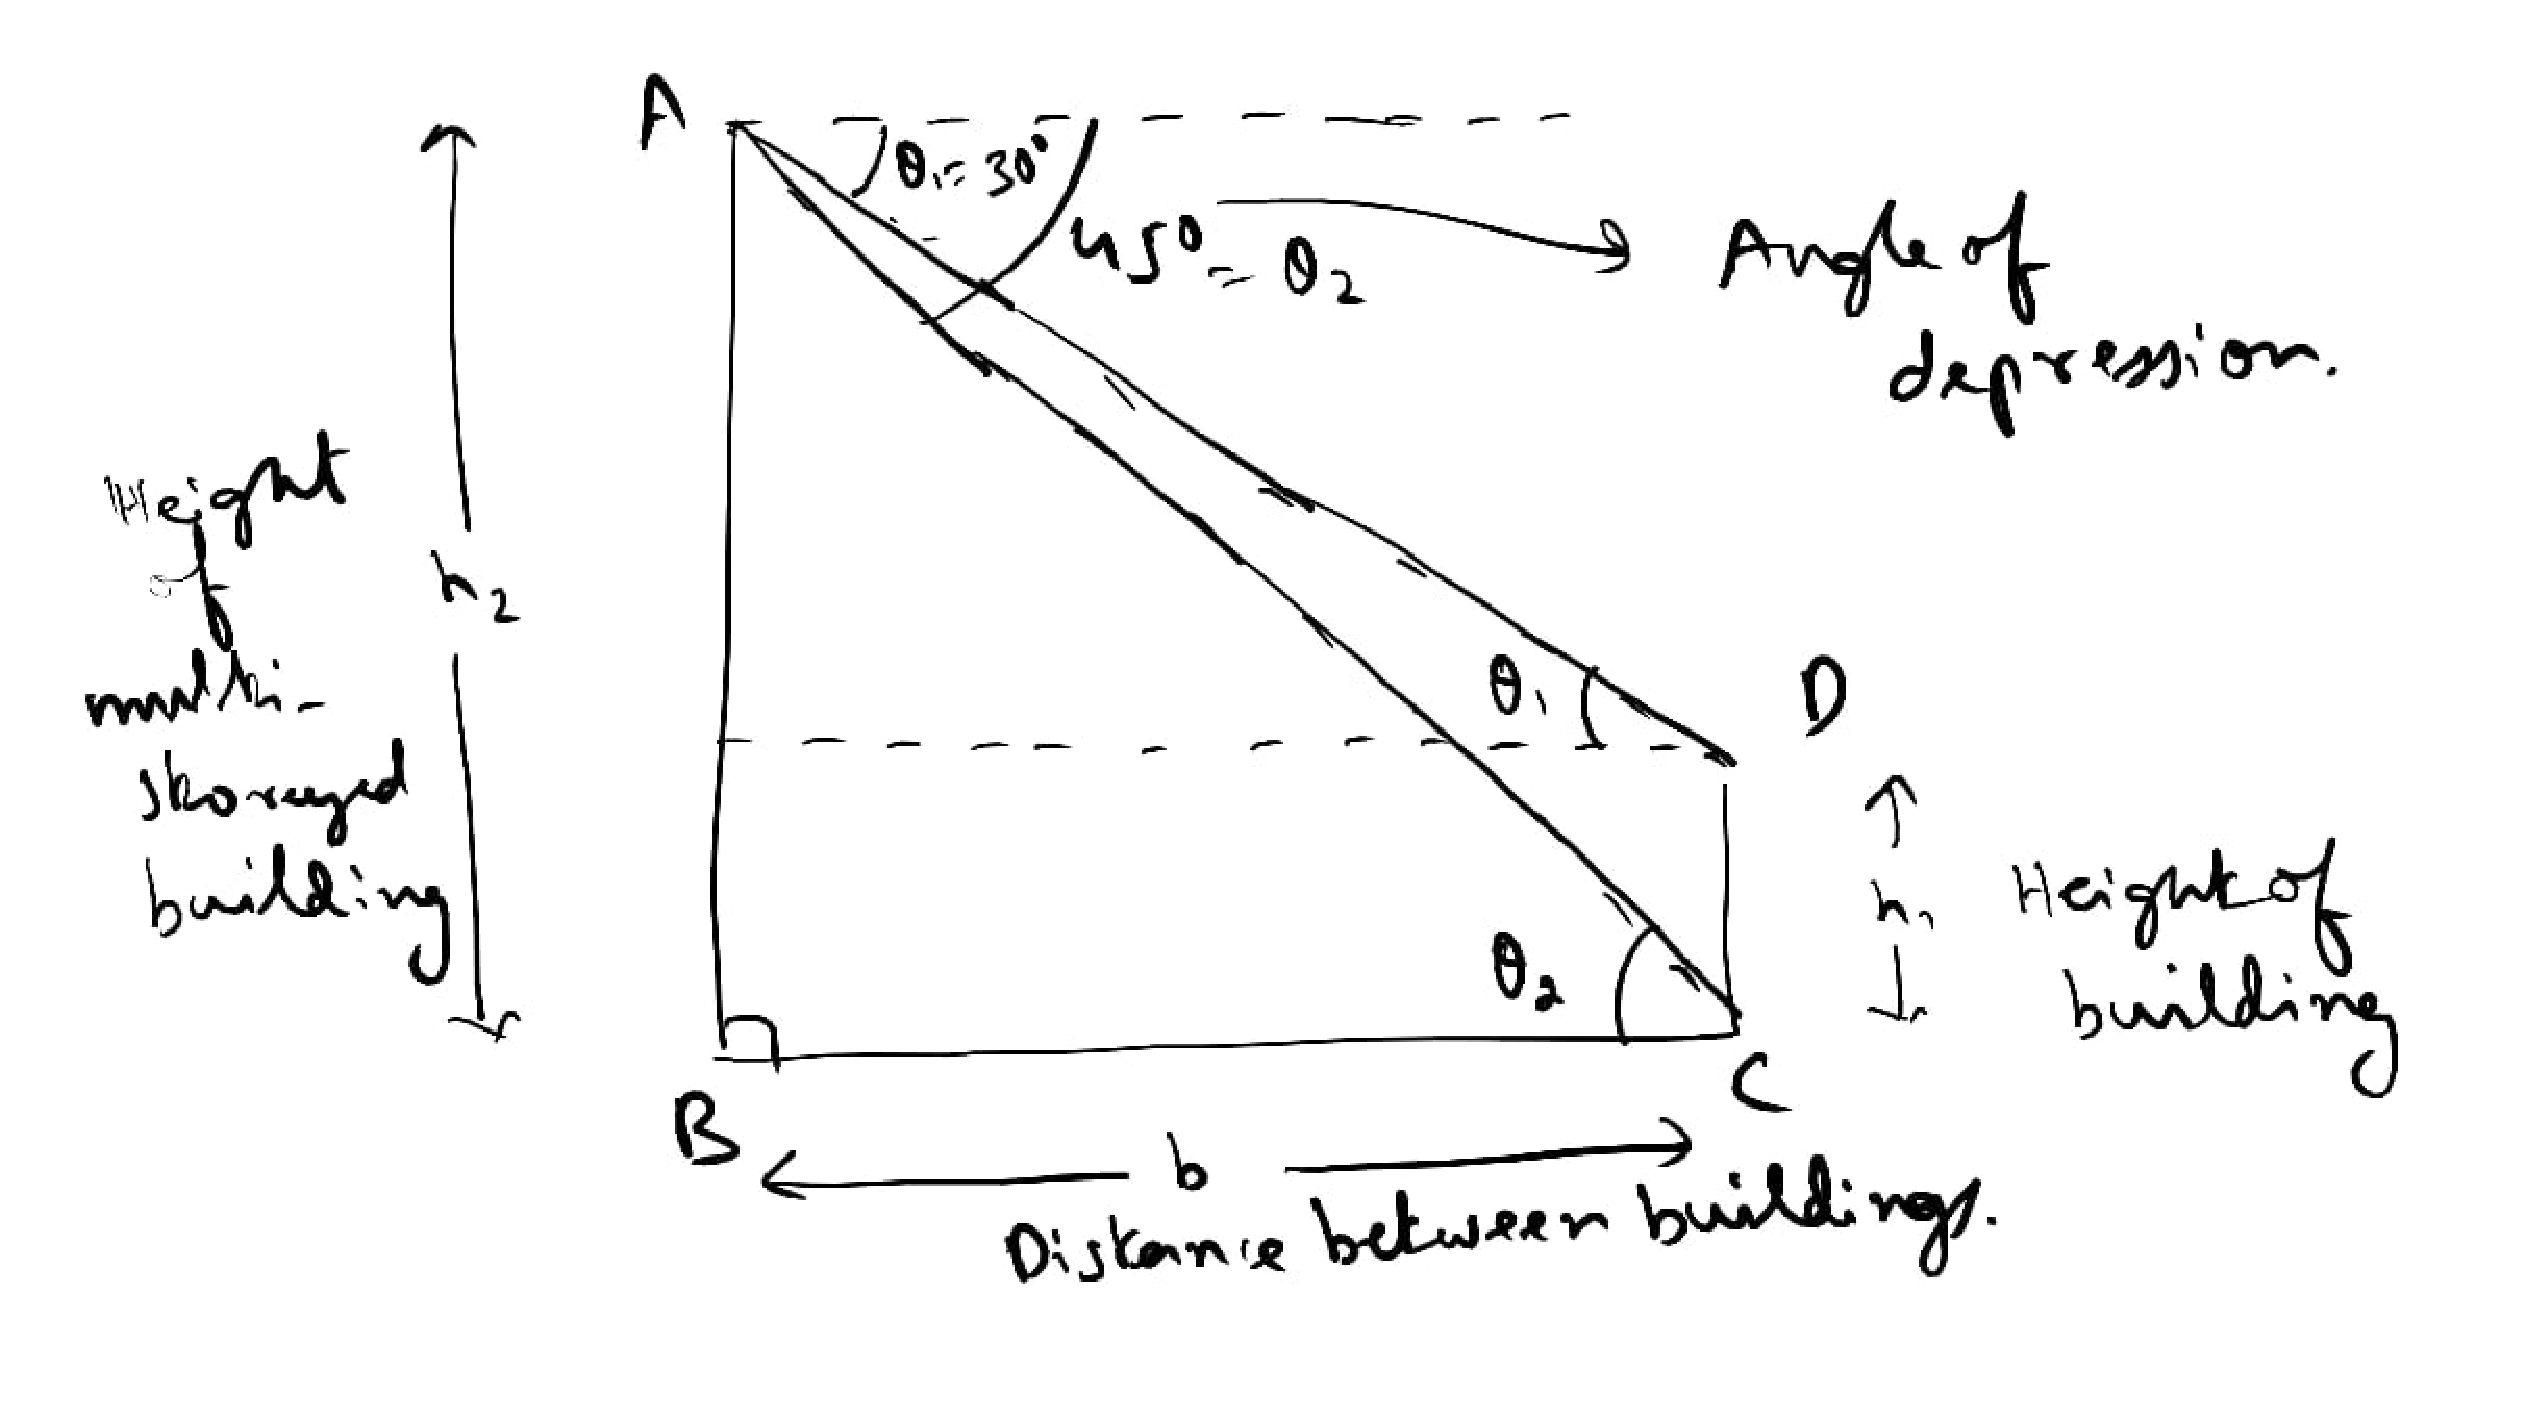
\includegraphics[width=\columnwidth]{./figs/Trig/pg6.eps}
%\caption{}
%\label{fig:trig_pg6}
%\end{figure}
%%
%\\
%\solution Fig. \ref{fig:trig_pg6} summarizes the problem. The objective is to find $h_2$ and $b$.  From the figure, 
%%
%\begin{align}
%h_2 &= b\tan \theta_2
%\\
%h_2-h_1 &= b\tan \theta_1
%\end{align}
%%
%which can be expressed as
%%
%\begin{align}
%\myvec{
% 1 & -\tan\theta_2 
%\\
% 1 & -\tan\theta_1
%}\myvec{h_2\\b}
%= h_1\myvec{0\\1}
%\end{align}
%%
%and solved.
\item A traffic signal board, indicating ‘SCHOOL AHEAD’, is an equilateral triangle with side 'a'. Find the area of the signal board, using Heron's formula. If its perimeter is 180 cm, what will be the area of the signal board?
	\iffalse
\item The triangular side walls of a flyover have been used for advertisements. The sides of the walls are 122 m, 22 m and 120 m. The advertisements yield an earning of \rupee 5000 per $m^2$ per year.  A company hired one o its walls for 3 months. How  much rent did it pay?
	\fi
\item There is a slide in a park. One of its side walls has been painted in some colour with a message ``KEEP THE PARK GREEN AND CLEAN". If the sides of the wall are 15 m, 11 m and 6 m, find the area painted in colour.
\item Find the area of a triangle two sides of which are 18cm and 10cm and the perimeter is 42cm.
\item Sides of a triangle are in the ratio of 12 : 17 : 25 and its perimeter is 540cm. Find its area. 
\item  An isosceles triangle has perimeter 30 cm and each of the equal sides is 12 cm. Find the area of the triangle.
\item A girl walks 4km west, then she walks 3km in a direction $30\degree$ east of north and stops.  Determine the girl's displacement from her initial point of departure.
%
\item A circus artist is climbing a 20m long rope, which is tightly stretched and tied from the top of a vertical pole to the ground.  Find the height of the pole, if the angle made by the rope with the ground level is 30$\degree$.
%
\item A tree breaks due to storm and the broken part bends so that the top of the tree touches the ground making an angle of 30$\degree$ with it.  The distance between the foot of the tree to the point where the top touches the ground is 8m.  Find the height of the tree.
%
\item A contractor plans to install two slides for the children to play in a park.  For the children below the age of 5 years, she prefers to have a slide whose top is at a height of 1.5m, and is inclined at an angle of 30$\degree$  to the ground, whereas for elder children she wants to have a steep slide at a height of 3m, and inclined at an angle of 60$\degree$ to the ground.  What should be the length of the slide in each case?
%
\item The angle of elevation of the top of a tower from a point on the ground, which is 30m away from the foot of the tower, is 30$\degree$.  Find the height of the tower.
%
\item A kite is flying at a height of 60m above the ground.  The string attached to the kite is temporarily tied to a point on the ground.  The inclination of the string with the ground is $60\degree$.  Find the length of the string, assuming that there is no slack in the string.
%
\item A 1.5m tall boy is standing at some distance from a 30m tall building.  The angle of elevation from his eyes to the top of the building increases from 30$\degree$
 to 60$\degree $ as he walks towards the building.  Find the distance he walked towards the building.

\item From a point on the ground, the angles of elevation of the bottom and the top of a transmission tower fixed at the top of a 20 m high building are 45$\degree$ and 60$\degree$ respectively. Find the height of the tower.

\item A statue, 1.6 m tall, stands on the top of a pedestal. From a point on the ground, the angle of elevation of the top of the statue is 60$\degree$ and from the same point the angle of elevation of the top of the pedestal is 45$\degree$. Find the height of the pedestal.
\item The angle of elevation of the top of a building from the foot of the tower is 30$\degree$ and the angle of elevation of the top of the tower from the foot of the building is 60$\degree$. If the tower is 50 m high, find the height of the building.
\item Two poles of equal heights are standing opposite each other on either side of the road, which is 80 m wide. From a point between them on the road, the angles of elevation of the top of the poles are 60$\degree$ and 30$\degree$, respectively. Find the height of the poles and the distances of the point from the poles.
\item A TV tower stands vertically on a bank of a canal. From a point on the other bank directly opposite the tower, the angle of elevation of the top of the tower is 60$\degree$. From another point 20 m away from this point on the line joing this point to the foot of the tower, the angle of elevation of the top of the tower is 30$\degree$. Find the height of the tower and the width of the canal.
\item From the top of a 7 m high building, the angle of elevation of the top of a cable tower is 60$\degree$ and the angle of depression of its foot is 45$\degree$. Determine the height of the tower.
\item As observed from the top of a 75 m high lighthouse from the sea-level, the angles of depression of two ships are 30$\degree$ and 45$\degree$. If one ship is exactly behind the other on the same side of the lighthouse, find the distance between the two ships.
\item A 1.2 m tall girl spots a balloon moving with the wind in a horizontal line at a height of 88.2 m from the ground. The angle of elevation of the balloon from the eyes of the girl at any instant is 60$\degree$. After some time, the angle of elevation reduces to 30$\degree$. Find the distance travelled by the balloon during the interval.
\item A straight highway leads to the foot of a tower. A man standing at the top of the tower observes a car at an angle of depression of 30$\degree$, which is approaching the foot of the tower with a uniform speed. Six seconds later, the angle of depression of the car is found to be 60$\degree$. Find the time taken by the car to reach the foot of the tower from this point.
\item The angles of elevation of the top of a tower from two points at a distance of 4 m and 9 m from the base of the tower and in the same straight line with it are complementary. Prove that the height of the tower is 6 m.
%
\item $E$ and $F$ are points on the sides  $PQ$  and PR respectively of a  $\triangle PQR$ . For each of the following cases, state whether $EF  \parallel  QR$ 
\begin{enumerate}
\item  $PE = 3.9 cm, EQ = 3 cm, PF = 3.6 cm$ and $FR = 2.4 cm $
\item  $PE = 4 cm, QE = 4.5 cm, PF = 8 cm$ and $RF = 9 cm $
\item   $PQ  = 1.28 cm, PR = 2.56 cm, PE = 0.18 cm$ and $PF = 0.36 cm$
\end{enumerate}
\item A girl of height 90 cm is walking away from the base of a lamp-post at a speed of 1.2 m/s. If the lamp is 3.6 m above the ground, find the length of her shadow after 4 seconds.
\item  $ \triangle  ODC \sim  \triangle  OBA, \angle BOC = 125 \degree$ and $\angle CDO = 70 \degree$. Find $\angle DOC, \angle DCO$ and $\angle OAB$.
\item  Nazima is fly fishing in a stream. The tip of her fishing rod is 1.8 m above the surface of the water and the fly at the end of the string rests on the water 3.6 m away and 2.4 m from a point directly under the tip of the rod. Assuming that her string (from the tip of her rod to the fly) is taut, how much string does she have out? If she pulls in the string at the rate of 5 cm per second, what will be the horizontal distance of the fly from her after 12 seconds?
%
\item  A vertical pole of length 6 m casts a shadow 4 m long on the ground and at the same time a tower casts a shadow 28 m long. Find the height of the tower.
\item Let  $\triangle  ABC  \sim   \triangle  DEF$ and their areas be, respectively, 64 $cm^2$ and 121 $cm^2$.  If $EF = 15.4 cm$, find BC.
\item A ladder is placed against a wall such that its foot is at a distance of 2.5 m from the wall and its top reaches a window 6 m above the ground. Find the length of the ladder.
\item Sides of triangles are given below. Determine which of them are right triangles. In case of a right triangle, write the length of its hypotenuse. 
\begin{enumerate}
\item  7 cm, 24 cm, 25 cm 
\item  3 cm, 8 cm, 6 cm 
\item  50 cm, 80 cm, 100 cm 
\item  13 cm, 12 cm, 5 cm
\end{enumerate}
\item  A ladder 10 m long reaches a window 8 m above the ground. Find the distance of the foot of the ladder from base of the wall.
\item  A guy wire attached to a vertical pole of height 18 m is 24 m long and has a stake attached to the other end. How far from the base of the pole should the stake be driven so that the wire will be taut?
\item  An aeroplane leaves an airport and flies due north at a speed of 1000 km per hour. At the same time, another aeroplane leaves the same airport and flies due west at a speed of 1200 km per hour. How far apart will be the two planes after $1\frac{1}{2}$ hours?
\item  Two poles of heights 6 m and 11 m stand on a plane ground. If the distance between the feet of the poles is 12 m, find the distance between their tops.
\item  In  $\triangle  ABC, AB = 6\sqrt{3} cm, AC = 12 cm$ and $BC = 6 cm$. Find the angle $B$.
%
\item A park, in the shape of a quadrilateral $ABCD$, has $\angle C = 90\degree, AB = 9 m, BC = 12 m, CD = 5 m$ and $ AD = 8 m$. How much area does it occupy?
2. Find the area of a quadrilateral $ABCD$ in which $AB = 3 cm, BC = 4 cm, CD = 4 cm, DA = 5 cm$ and $AC = 5 cm$.
\item A triangle and a parallelogram have the same base and the same area. If the sides of the triangle are 26 cm, 28 cm and 30 cm, and the parallelogram stands on the base 28 cm, find the height of the parallelogram.
\item A rhombus shaped field has green grass for 18 cows to graze. If each side of the rhombus is 30 m and its longer diagonal is 48 m, how much area of grass field will each cow be getting?
\item A field is in the shape of a trapezium whose parallel sides are 25 m and 10 m. The non-parallel sides are 14 m and 13 m. Find the area of the field.
%
\item $ABCD$ is a parallelogram, $AE  \perp  DC$ and $CF  \perp  AD$. If $AB = 16 cm$, $AE = 8$ cm and $CF = 10$ cm, find $AD$.
\item Kamla has a triangular field with sides 240 m, 200 m, 360 m, where she grew wheat. In another triangular field with sides 240 m, 320 m, 400 m adjacent to the previous field, she wanted to grow potatoes and onions. She divided the field in two parts by joining the mid-point of the longest side to the opposite vertex and grew patatoes in one part and onions in the other part. Draw the figure for this problem.  How much area (in hectares) has been used for wheat, potatoes and onions? (1 hectare = 10000 $m^2$).
\item Students of a school staged a rally for cleanliness campaign. They walked through the lanes in two groups. One group walked through the lanes AB, BC and CA; while the other through AC, CD and DA. Then they cleaned the area enclosed within their lanes. If AB = 9 m, BC = 40 m, CD = 15 m, DA = 28 m and $\angle B = 90\degree$, which group cleaned more area and by how much? Draw the corresponding figure.  Find the total area cleaned by the students (neglecting the width of the lanes). 
%
\item Sanya has a piece of land which is in the shape of a rhombus. She wants her one daughter and one son to work on the land and produce different crops. She divided the land in two equal parts. If the perimeter of the land is 400 m and one of the diagonals is 160 m, how much area each of them will get for their crops? Draw the rhombus.
%
\item Three girls Reshma, Salma and Mandip are playing a game by standing on a circle of radius 5m drawn in a park. Reshma throws a ball to Salma, Salma to Mandip, Mandip to Reshma. If the distance between Reshma and Salma and between Salma and Mandip is 6m each, what is the distance between Reshma and Mandip?
\item A circular park of radius 20m is situated in a colony. Three boys Ankur, Syed and David are sitting at equal distance on its boundary each having a toy telephone in his hands to talk each other. Find the length of the string of each phone.
    \item The longest side of a triangle is 3 times the shortest side and the third side is 2 cm shorter than the longest side. If the perimeter of the triangle is at least 61 cm, find the minimum length of the shortest side.
\item A rectangular park is to be designed whose breadth is 3 m less than its length. Its area is to be 4 square metres more than the area of a park that has already been made in the shape of an isosceles triangle with its base as the breadth of the rectangular park and of altitude 12 m. Find its length and breadth.
\item The area of a rectangular plot is 528 $m^2$
. The length of the plot (in metres) is one more than twice its breadth. We need to find the length and breadth of the plot.
%
\item  The altitude of a right triangle is 7 cm less than its base. If the hypotenuse is 13 cm, find the other two sides.
%
\item The diagonal of a rectangular field is 60 metres more than the shorter side. If the longer side is 30 metres more than the shorter side, find the sides of the field.
\item Is it possible to design a rectangular mango grove whose length is twice its breadth, and the area is 800 $m^2$
? If so, find its length and breadth.
%
\item Is it possible to design a rectangular park of perimeter 80 m and area 400 $m^2$ If so, find  its length and breadth.
\item On an open ground, a motorist follows a track that turns to his left by an angle of 600 after every 500 m. Starting from a given turn, specify the displacement of the motorist at the third, sixth and eighth turn. Compare the magnitude of the displacement with the total path length covered by the motorist in each case.
\item A passenger arriving in a new town wishes to go from the station to a hotel located 10 km away on a straight road from the station. A dishonest cabman takes him along a circuitous path 23 km long and reaches the hotel in 28 min. What is 
\begin{enumerate}
\item  the average speed of the taxi, 
\item  the magnitude of average velocity ? Are the two equal ?

\end{enumerate}
\item An aircraft is flying at a height of 3400 m above the ground. If the angle subtended at a ground observation point by the aircraft positions 10.0 s apart is 30$\degree$, what is the speed of the aircraft ?
\item Two identical billiard balls strike a rigid wall with the same speed but at different angles, and get reflected without any change in speed, as shown in Fig. \ref{fig:5.6}. What is 
\begin{enumerate}
\item  the direction of the force on the wall due to each ball? 
\item the ratio of the magnitudes of impulses imparted to the balls by the wall ?
\end{enumerate}
\begin{figure}[!ht]
\centering
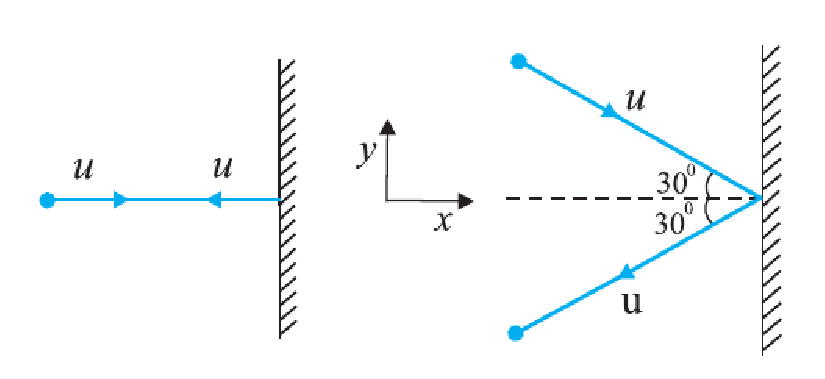
\includegraphics[width=\columnwidth]{./figs/11-1/5/5.6.eps}
\caption{}
\label{fig:5.6}
\end{figure} 

\item See Fig. \ref{fig:5.8}. A mass of 6 kg is suspended by a rope of length 2 m from the ceiling. A force of 50 N in the horizontal direction is applied at the midpoint P of the rope, as shown. What is the angle the rope makes with the vertical in equilibrium ? (Take g = 10 $m s^{-2}$).
\begin{figure}[!ht]
\centering
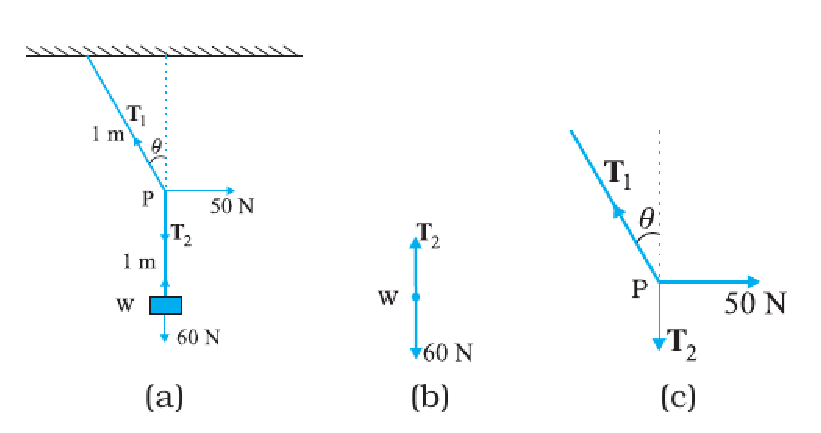
\includegraphics[width=\columnwidth]{./figs/11-1/5/5.8.eps}
\caption{}
\label{fig:5.8}
\end{figure} 
\item See Fig. \ref{fig:5.11}. A mass of 4 kg rests on a horizontal plane. The plane is gradually inclined until at an angle $\theta = 15\degree$ with the horizontal, the mass just begins to slide. What is the coefficient of static friction between the block and the surface ?
\begin{figure}[!ht]
\centering
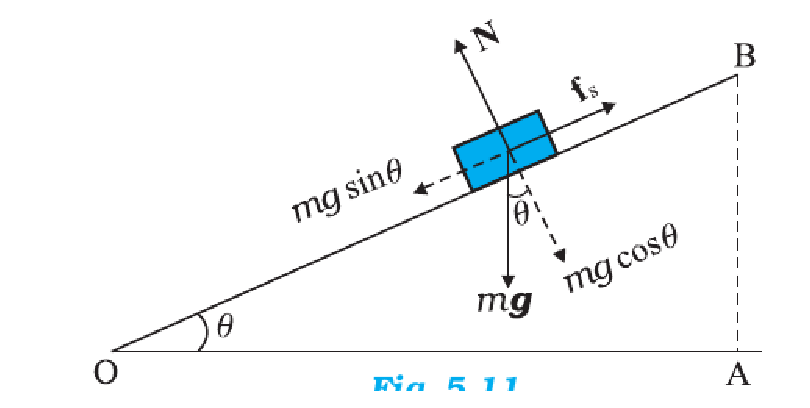
\includegraphics[width=\columnwidth]{./figs/11-1/5/5.11.eps}
\caption{}
\label{fig:5.11}
\end{figure} 
\item A cyclist speeding at 18 km/h on a level road takes a sharp circular turn of radius 3 m without reducing the speed. The co-efficient of static friction between the tyres and the road is 0.1. Will the cyclist slip while taking the turn?
\item A circular racetrack of radius 300 m is banked at an angle of 15$\degree$. If the coefficient of friction between the wheels of a race-car and the road is 0.2, what is the 
\begin{enumerate}
\item  optimum speed of the racecar to avoid wear and tear on its tyres, and 
\item  maximum permissible speed to avoid slipping ?
\end{enumerate}
\item An aircraft executes a horizontal loop at a speed of 720 km/h with its wings banked at 15$\degree$. What is the radius of the loop ?
\item A train runs along an unbanked circular track of radius 30 m at a speed of 54 km/h. The mass of the train is $10^6$
kg. What provides the centripetal force required for this
purpose - The engine or the rails ? What is the angle of banking required to prevent wearing out of the rail ?
\item A disc revolves with a speed of $33 \frac{1}{ 3}$ rev/min 
 and has a radius of 15 cm. Two coins are
placed at 4 cm and 14 cm away from the centre of the record. If the co-efficient of friction between the coins and the record is 0.15, which of the coins will revolve with the record ?
\item A 70 kg man stands in contact against the inner wall of a hollow cylindrical drum of radius 3 m rotating about its vertical axis with 200 rev/min. The coefficient of friction between the wall and his clothing is 0.15. What is the minimum rotational speed of the cylinder to enable the man to remain stuck to the wall (without falling) when the floor is suddenly removed ?
\item A thin circular loop of radius R rotates about its vertical diameter with an angular frequency $\omega$. Show that a small bead on the wire loop remains at its lowermost point for $\omega \le \sqrt{\frac{g}{R}}$ . What is the angle made by the radius vector joining the centre to the bead with the vertical downward direction for $\omega = \sqrt{\frac{2g}{R}}$  ? Neglect friction.
\item A stone of mass 0.25 kg tied to the end of a string is whirled round in a circle of radius 1.5 m with a speed of 40 rev./min in a horizontal plane. What is the tension in the string ? What is the maximum speed with which the stone can be whirled around if the string can withstand a maximum tension of 200 N ?
\item A woman pushes a trunk on a railway platform which has a rough surface. She applies a force of 100 N over a distance of 10 m. Thereafter, she gets progressively tired and her applied force reduces linearly with distance to 50 N. The total distance through which the trunk has been moved is 20 m. Plot the force applied by the woman and the frictional force, which is 50 N versus displacement. Calculate the work done by the two forces over 20 m.
\item A bob of mass m is suspended by a light string of length L . It is imparted a horizontal velocity $v_o$
such that it completes a semi-circular trajectory in the vertical plane with the string becoming slack only on reaching the topmost point, C. This is shown in Fig. \ref{fig:6.6}. Obtain an expression for 
\begin{enumerate}
\item  vo; 
\item  the speeds at points B and C; 
\item  the ratio of the kinetic energies ($K_B/K_C$) at B and C. 
\end{enumerate}
Comment on the nature
of the trajectory of the bob after it reaches the point C.
\begin{figure}[!ht]
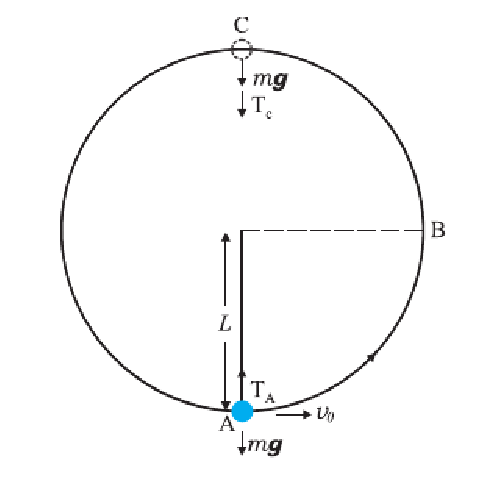
\includegraphics[width=\columnwidth]{./figs/11-1/6/6.6.eps}
\caption{}
\label{fig:6.6}
\end{figure}
\item The bob A of a pendulum released from 30\degree to the
vertical hits another bob B of the same mass at rest on a table as shown in Fig. \ref{fig:6.15}. How high does the bob A rise after the collision? Neglect the size of the bobs and assume the collision to be elastic.
\begin{figure}[!ht]
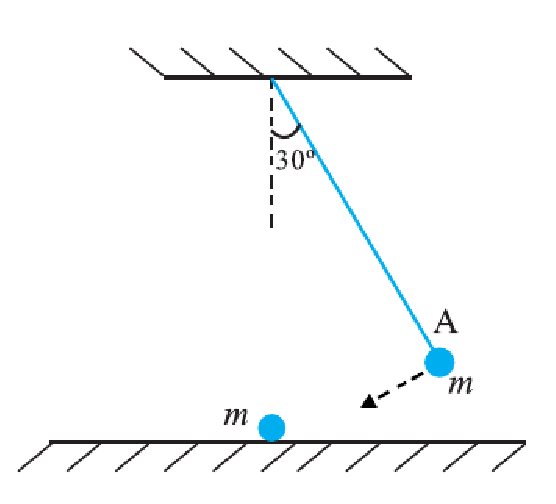
\includegraphics[width=\columnwidth]{./figs/11-1/6/6.15.eps}
\caption{}
\label{fig:6.15}
\end{figure}
%
\item The bob of a pendulum is released from a horizontal position. If the length of the pendulum is 1.5 m, what is the speed with which the bob arrives at the lowermost point, given that it dissipated 5\% of its initial energy against air resistance ?
\item The blades of a windmill sweep out a circle of area A. 
\begin{enumerate}[label=(\alph*)]
\item  If the wind flows at a velocity v perpendicular to the circle, what is the mass of the air passing through it in time t ? 
\item  What is the kinetic energy of the air ? 
\item  Assume that the windmill converts 25\% of the wind’s energy into electrical energy, and that $A = 30 m^2, v = 36km/h$ and the density of air is $1.2 kg m^{-3}$. What is the electrical power produced ?
\end{enumerate}
\item A bullet of mass 0.012 kg and horizontal speed $70 m s^{-1}$.
strikes a block of wood of
mass 0.4 kg and instantly comes to rest with respect to the block. The block is suspended from the ceiling by means of thin wires. Calculate the height to which the block rises. Also, estimate the amount of heat produced in the block.
\item Two inclined frictionless tracks, one gradual and the other steep meet at A from where two stones are allowed to slide down from rest, one on each track (Fig. \ref{fig:6.16}). Will the stones reach the bottom at the same time? Will they reach there with the same speed? Explain. Given $\theta_1 = 30\degree\theta_2 = 60\degree$  and $h = 10m$, what are the speeds and times taken by the two stones?
\begin{figure}[!ht]
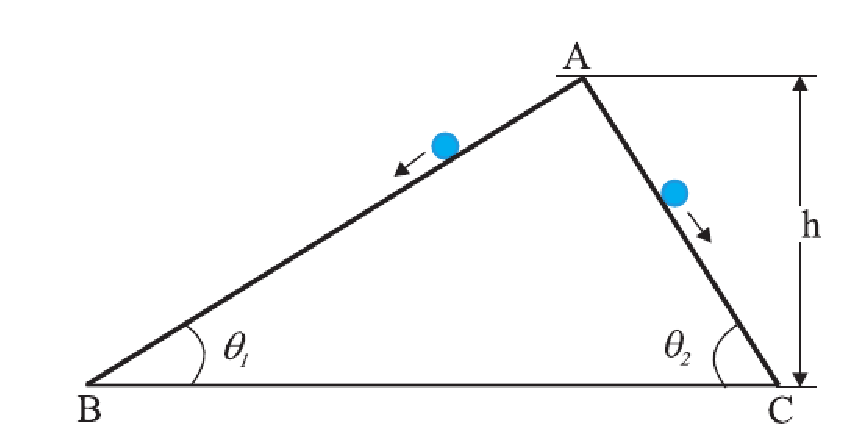
\includegraphics[width=\columnwidth]{./figs/11-1/6/6.16.eps}
\caption{}
\label{fig:6.16}
\end{figure}
\item  A 1 kg block situated on a rough incline is connected to a spring of spring constant 100 N m–1
as shown in Fig. \ref{fig:6.17}. The block is released from rest with the spring in the
unstretched position. The block moves 10 cm down the incline before coming to rest. Find the coefficient of friction between the block and the incline. Assume that the
spring has a negligible mass and the pulley is frictionless.
\begin{figure}[!ht]
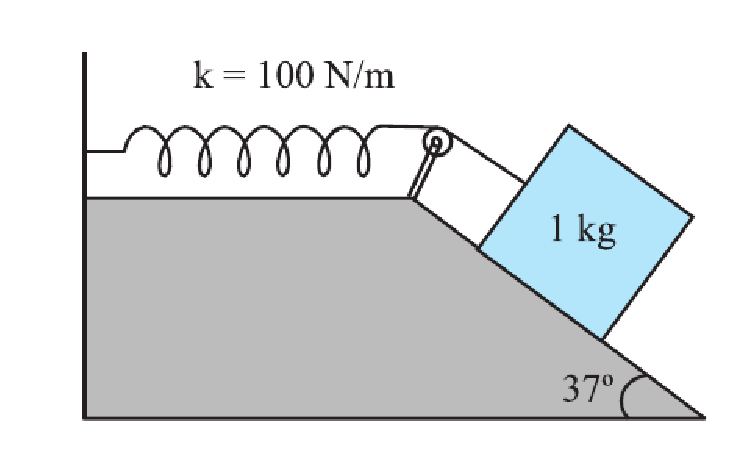
\includegraphics[width=\columnwidth]{./figs/11-1/6/6.17.eps}
\caption{}
\label{fig:6.17}
\end{figure}
\item Find the centre of mass of three particles at the vertices of an equilateral triangle. The masses of the particles are 100g, 150g, and 200g respectively. Each side of the equilateral triangle is 0.5m long.
\item Find the centre of mass of a triangular lamina.
\item Find the centre of mass of a uniform L-shaped lamina (a thin flat plate) with dimensions as shown in Fig. \ref{fig:7.11}. The mass of the lamina is 3 kg.
\begin{figure}[!ht]
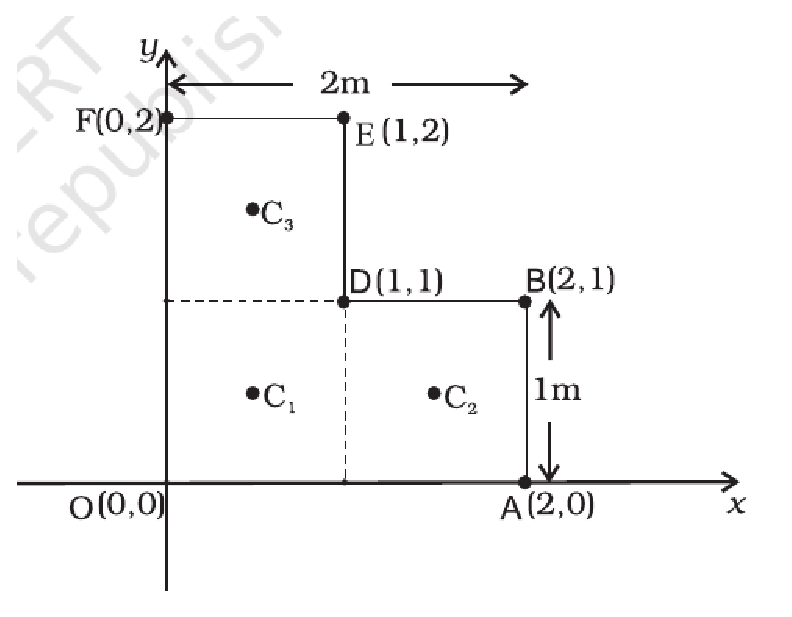
\includegraphics[width=\columnwidth]{./figs/11-1/7/7.11.eps}
\caption{}
\label{fig:7.11}
\end{figure}
\item A metal bar 70 cm long and 4.00 kg in mass supported on two knife-edges placed 10 cm from each end. A 6.00 kg load is suspended at 30 cm from one end. Find the reactions at the knifeedges. (Assume the bar to be of uniform cross section and homogeneous.)
\item A 3m long ladder weighing 20 kg leans on a frictionless wall. Its feet rest on the floor 1 m from the wall as shown in Fig. \ref{fig:7.27}. Find the reaction forces of the wall and the floor.
\begin{figure}[!ht]
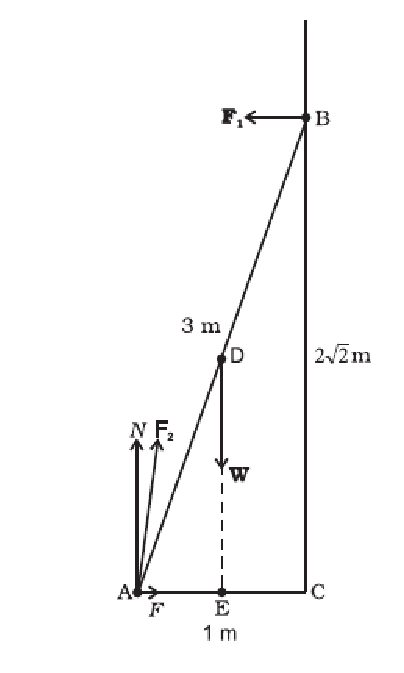
\includegraphics[width=\columnwidth]{./figs/11-1/7/7.27.eps}
\caption{}
\label{fig:7.27}
\end{figure}
\item What is the moment of inertia of a rod of mass M, length l about an axis perpendicular to it through one end?
\item What is the moment of inertia of a ring about a tangent to the circle of the ring?
\item  A cord of negligible mass is wound round the rim of a fly wheel of mass 20 kg and radius 20 cm. A steady pull of 25 N is applied on the cord as shown in Fig. \ref{fig:7.35}. The flywheel is mounted on a horizontal axle with frictionless bearings.
\begin{figure}[!ht]
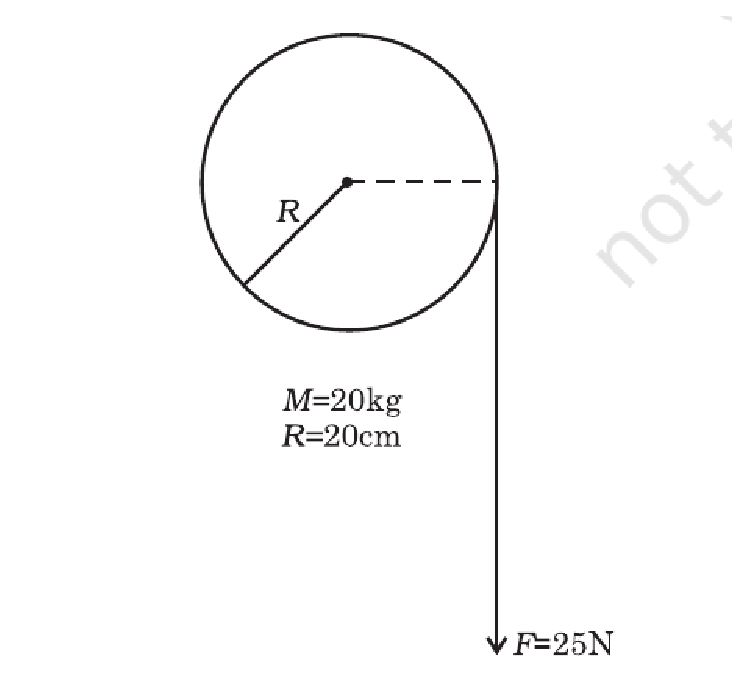
\includegraphics[width=\columnwidth]{./figs/11-1/7/7.35.eps}
\caption{}
\label{fig:7.35}
\end{figure}
\begin{enumerate}[label=(\alph*)]
\item  Compute the angular acceleration of the wheel.
\item  Find the work done by the pull, when 2m of the cord is unwound.
\item  Find also the kinetic energy of the wheel at this point. Assume that the wheel starts from rest.
\item  Compare answers to parts (b) and (c).
\end{enumerate}
\item Three bodies, a ring, a solid cylinder and a solid sphere roll down the same inclined plane without slipping. They start from rest. The radii of the bodies are identical. Which of the bodies reaches the ground with maximum velocity?
	\iffalse
\item In the HCl molecule, the separation between the nuclei of the two atoms is about 
1.27 \si{\angstrom} (1 \si{\angstrom} = $10^{-10}$ m). 
Find the approximate location of the CM of the molecule, given that a chlorine atom is about 35.5 times as massive as a hydrogen atom and nearly all the mass of an atom is concentrated in its nucleus.
\fi
\item A non-uniform bar of weight W is suspended at rest by two strings of negligible weight as shown in Fig. \ref{fig:7.39}. The angles made by the strings with the vertical are 36.9$\degree$ and 53.1$\degree$ respectively. The bar is 2 m long. Calculate the distance d of the centre of gravity of the bar from its left end.
\begin{figure}[!ht]
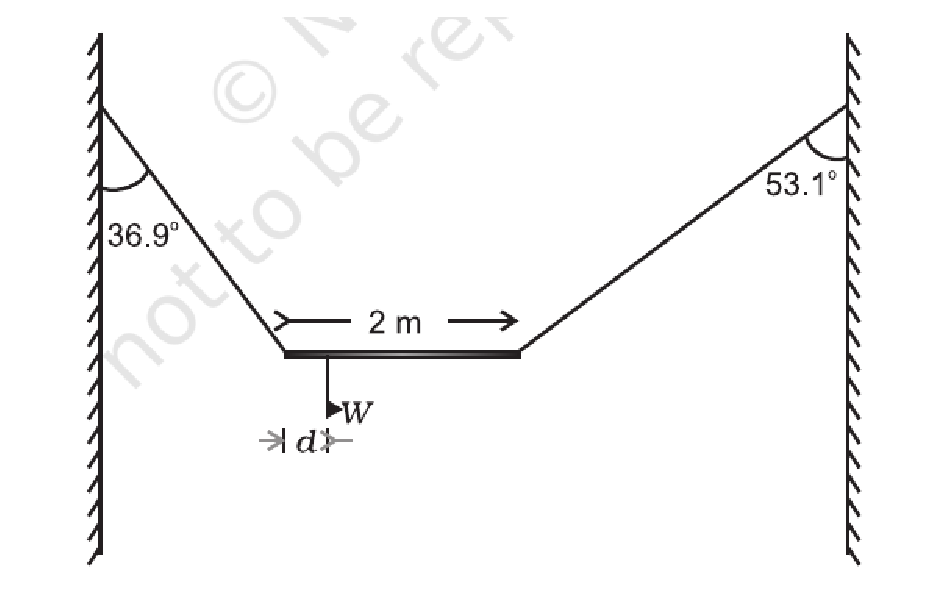
\includegraphics[width=\columnwidth]{./figs/11-1/7/7.39.eps}
\caption{}
\label{fig:7.39}
\end{figure}
\item A car weighs 1800 kg. The distance between its front and back axles is 1.8 m. Its centre of gravity is 1.05 m behind the front axle. Determine the force exerted by the level ground on each front wheel and each back wheel.
\item 
\begin{enumerate}[label=(\alph*)]
\item Find the moment of inertia of a sphere about a tangent to the sphere, given the moment of inertia of the sphere about any of its diameters to be $\frac{2MR^2}{5}$ where M is the mass of the sphere and R is the radius of the sphere.
\item  Given the moment of inertia of a disc of mass M and radius R about any of its diameters to be $\frac{MR^2}{4}$, find its moment of inertia about an axis normal to the
disc and passing through a point on its edge. 
\end{enumerate}
\item Torques of equal magnitude are applied to a hollow cylinder and a solid sphere, both having the same mass and radius. The cylinder is free to rotate about its standard axis of symmetry, and the sphere is free to rotate about an axis passing through its centre. Which of the two will acquire a greater angular speed after a given time.
\item A solid cylinder of mass 20 kg rotates about its axis with angular speed 100 $rad s^{-1}$. The radius of the cylinder is 0.25 m. What is the kinetic energy associated with the rotation of the cylinder? What is the magnitude of angular momentum of the cylinder about its axis?
\item 
\begin{enumerate}[label=(\alph*)]

\item  A child stands at the centre of a turntable with his two arms outstretched. The turntable is set rotating with an angular speed of 40 rev/min. How much is the angular speed of the child if he folds his hands back and thereby reduces his moment of inertia to 2/5 times the initial value ? Assume that the turntable rotates without friction.
\item Show that the child's new kinetic energy of rotation is more than the initial kinetic energy of rotation. How do you account for this increase in kinetic energy?
\end{enumerate}
\item  A rope of negligible mass is wound round a hollow cylinder of mass 3 kg and radius 40 cm. What is the angular acceleration of the cylinder if the rope is pulled with a force of 30 N ? What is the linear acceleration of the rope ? Assume that there is no slipping.
\item  To maintain a rotor at a uniform angular speed of 200 $rad s^{-1}$, an engine needs to transmit a torque of 180 N m. What is the power required by the engine ? (Note: uniform angular velocity in the absence of friction implies zero torque. In practice, applied torque is needed to counter frictional torque). Assume that the engine is 100\% efficient.
\item  From a uniform disk of radius R, a circular hole of radius R/2 is cut out. The centre of the hole is at R/2 from the centre of the original disc. Locate the centre of gravity of the resulting flat body.
\item  A metre stick is balanced on a knife edge at its centre. When two coins, each of mass 5 g are put one on top of the other at the 12.0 cm mark, the stick is found to be balanced at 45.0 cm. What is the mass of the metre stick?
\item A solid sphere rolls down two different inclined planes of the same heights but different angles of inclination. 
\begin{enumerate}[label=(\alph*)]
\item  Will it reach the bottom with the same speed in each case? 
\item  Will it take longer to roll down one plane than the other? 
\item  If so, which one and why?
\end{enumerate}
\item  A hoop of radius 2 m weighs 100 kg. It rolls along a horizontal floor so that its centre of mass has a speed of 20 cm/s. How much work has to be done to stop it? 
\item  The oxygen molecule has a mass of $5.30  \times  10^{-26} $ kg and a moment of inertia of
$1.94 \times 10^{-46} kg m^2$ about an axis through its centre perpendicular to the lines joining
the two atoms. Suppose the mean speed of such a molecule in a gas is 500 m/s and that its kinetic energy of rotation is two thirds of its kinetic energy of translation. Find the average angular velocity of the molecule.
\item  A solid cylinder rolls up an inclined plane of angle of inclination 30$\degree$. At the bottom of the inclined plane the centre of mass of the cylinder has a speed of 5 m/s. 
\begin{enumerate}[label=(\alph*)]
\item How far will the cylinder go up the plane? 
\item  How long will it take to return to the bottom?
\end{enumerate}
\item  As shown in Fig. \ref{fig:7.40}, the two sides of a step ladder BA and CA are 1.6 m long and hinged at A. A rope DE, 0.5 m is tied half way up. A weight 40 kg is suspended from a point F, 1.2 m from B along the ladder BA. Assuming the floor to be frictionless and neglecting the weight of the ladder, find the tension in the rope and forces exerted by the floor on the ladder. (Take $g = 9.8 m/s^2$
) (Hint: Consider the equilibrium of each side of the ladder separately.) 
\begin{figure}[!ht]
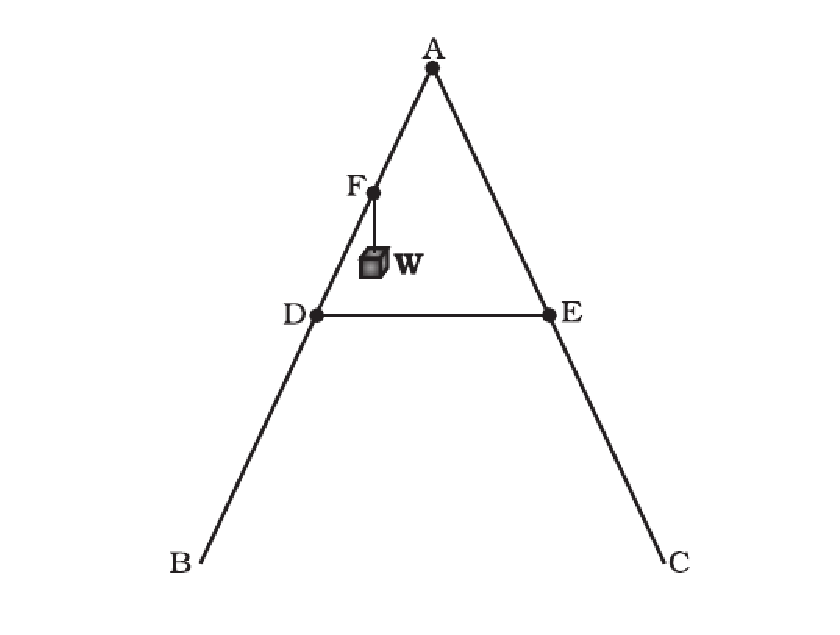
\includegraphics[width=\columnwidth]{./figs/11-1/7/7.40.eps}
\caption{}
\label{fig:7.40}
\end{figure}
%
\item A man stands on a rotating platform, with his arms stretched horizontally holding a 5 kg weight in each hand. The angular speed of the platform is 30 revolutions per minute. The man then brings his arms close to his body with the distance of each weight from the axis changing from 90cm to 20cm. The moment of inertia of the man together with the platform may be taken to be constant and equal to 7.6 $kg m^2$.
\begin{enumerate}[label=(\alph*)]
\item  What is his new angular speed? (Neglect friction.) 
\item  Is kinetic energy conserved in the process? If not, from where does the change come about?
\end{enumerate}
\item A bullet of mass 10 g and speed 500 m/s is fired into a door and gets embedded exactly at the centre of the door. The door is 1.0 m wide and weighs 12 kg. It is hinged at one end and rotates about a vertical axis practically without friction. Find the angular speed of the door just after the bullet embeds into it. (Hint: The moment of inertia of the door about the vertical axis at one end is $\frac{ML^2}{3}$.)
\item  Two discs of moments of inertia $I_1$ and $I_2$ about their respective axes (normal to the disc and passing through the centre), and rotating with angular speeds $\omega_1$ and $\omega_2$ are brought into contact face to face with their axes of rotation coincident. 
\begin{enumerate}[label=(\alph*)]
\item  What is the angular speed of the two-disc system? 
\item  Show that the kinetic energy of the combined system is less than the sum of the initial kinetic energies of the two discs. How do you account for this loss in energy? Take $\omega_1 \ne \omega_2$.
\end{enumerate}

\item Prove the result that the velocity v of translation of a rolling body (like a ring, disc, cylinder or sphere) at the bottom of an inclined plane of a height h is given by
\begin{align}
v^2 = \frac{2gh}{1+\frac{k^2}{R^2}}
\end{align}
using dynamical consideration (i.e. by consideration of forces and torques). Note k is the radius of gyration of the body about its symmetry axis, and R is the radius of the body. The body starts from rest at the top of the plane.
\item A disc rotating about its axis with angular speed $\omega_0$ is placed lightly (without any translational push) on a perfectly frictionless table. The radius of the disc is R. What are the linear velocities of the points A, B and C on the disc shown in Fig. \ref{fig:7.41}? Will the disc roll in the direction indicated ?
\begin{figure}[!ht]
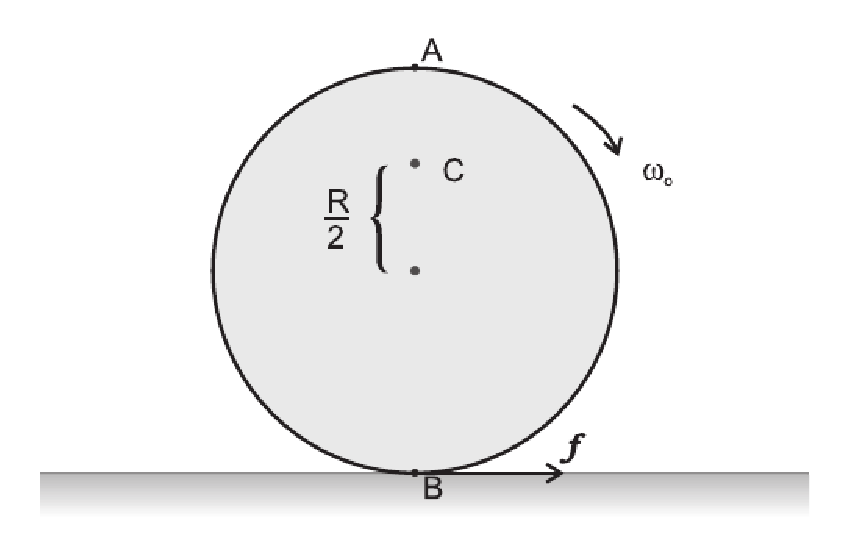
\includegraphics[width=\columnwidth]{./figs/11-1/7/7.41.eps}
\caption{}
\label{fig:7.41}
\end{figure}
\item Explain why friction is necessary to make the disc in Fig. \ref{fig:7.41} roll in the direction indicated. 
\begin{enumerate}[label=(\alph*)]
\item  Give the direction of frictional force at B, and the sense of frictional torque, before perfect rolling begins.
\item  What is the force of friction after perfect rolling begins ?
\end{enumerate}
\item  A solid disc and a ring, both of radius 10 cm are placed on a horizontal table simultaneously, with initial angular speed equal to 10 $\pi rad s^{-1}$ . Which of the two will start to roll earlier ? The coefficient of kinetic friction is $\mu_k$
= 0.2.
\item  A cylinder of mass 10 kg and radius 15 cm is rolling perfectly on a plane of inclination 30\degree. The coefficient of static friction $\mu_s$ = 0.25. 
\begin{enumerate}[label=(\alph*)]
\item  How much is the force of friction acting on the cylinder ? 
\item  What is the work done against friction during rolling ? 
\item  If the inclination $\theta$ of the plane is increased, at what value of $\theta$ does the cylinder begin to skid, and not roll perfectly ?
\end{enumerate}
\item Three equal masses of m kg each are fixed at the vertices of an
equilateral triangle ABC. 
\begin{enumerate}[label=(\alph*)]
\item  What is the force acting on a mass 2m placed at the centroid G of the triangle? 
\item  What is the force if the mass at the vertex A is doubled ? Take AG = BG = CG = 1 m (see Fig. \ref{fig:8.5})
\end{enumerate}
\begin{figure}[!ht]
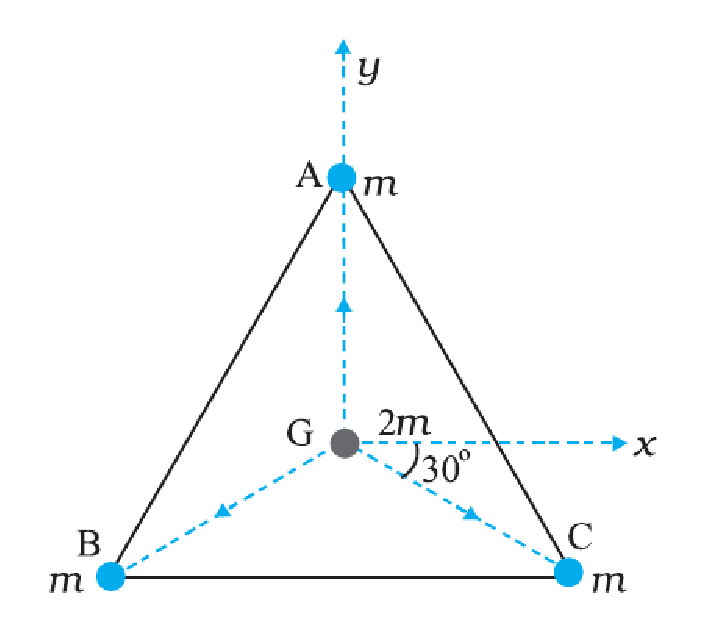
\includegraphics[width=\columnwidth]{./figs/11-1/8/8.5.eps}
\caption{}
\label{fig:8.5}
\end{figure}
\item Find the potential energy of a system of four particles placed at the vertices of a square of side $l$. Also obtain the potential at the centre of the square.
\item Two uniform solid spheres of equal radii R, but mass M and 4 M have a centre to centre separation 6 R, as shown in Fig. \ref{fig:8.10}. The two spheres are held fixed. A projectile of mass m is projected from the surface of the sphere of mass M directly towards the centre of the second sphere. Obtain an expression for the minimum speed v of the projectile so that it reaches the surface of the second sphere.
\begin{figure}[!ht]
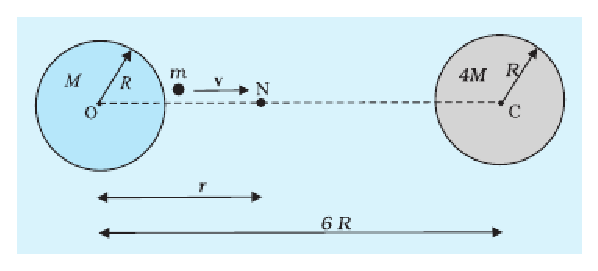
\includegraphics[width=\columnwidth]{./figs/11-1/8/8.10.eps}
\caption{}
\label{fig:8.10}
\end{figure}
\end{enumerate}


\iffalse
%\include{ch02} 
\backmatter
\appendix
\chapter{Area of a Circle}
%
%
\renewcommand{\theequation}{\theenumi}
\begin{enumerate}[label=\arabic*.,ref=\thesubsection.\theenumi]
\numberwithin{equation}{enumi}
%
%
\item
	The diameter of a circle is the chord that divides the circle into two equal parts. The diameter is equal to twice the radius
%
%	%
\item The ratio of the perimeter of a circle to its diameter is $\pi$.
\label{prob:circ_peri_dia}
\item {\em Radian} is a another unit of the angle defined by
%
\begin{align}
\pi \text{ radians} = 180 \degree
\end{align}
%
\item
	In Fig. \ref{ch5_polygon_def}, 6 congruent triangles are arranged in a circular fashion.  Such a figure is known as a regular hexagon.  In general, $n$ number of traingles can be arranged to form a regular polygon.
\begin{figure}[!ht]
	\begin{center}
		
		%\includegraphics[width=\columnwidth]{./figs/ch5_polygon_def}
		%\vspace*{-10cm}
		\resizebox{\columnwidth}{!}{\begin{tikzpicture}
[scale =2,>=stealth,point/.style = {draw, circle, fill = black, inner sep = 1pt},]

\node (O) at (0,0)[point,label=above :$O$] {};
\node (F) at (-3,0)[point,label=left :$F$] {};
\node (C) at (3,0)[point,label=right :$C$] {};
\node (E) at (-1.5,3)[point,label=above :$E$] {};
\node (D) at (1.5,3)[point,label=above :$D$] {};
\node (A) at (-1.5,-3)[point,label=below :$A$] {};
\node (B) at (1.5,-3)[point,label=below :$B$] {};
\draw (A)--(D);
\draw (B)--(E);
\draw (F)--(C);
\draw (A)--(F);
\draw (F)--(E);
\draw (E)--(D);
\draw (D)--(C);
\draw (C)--(B);
\draw (B)--(A);

\tkzMarkAngle[size=.2](F,O,A);
\tkzMarkAngle[size=.22](E,O,F);
\tkzMarkAngle[size=.26](D,O,E);
\tkzMarkAngle[size=.2](C,O,D);
\tkzMarkAngle[size=.22](B,O,C);
\tkzMarkAngle[size=.26](A,O,B);

\node [above] at (-0.8,-1.5){$r$};
\node [above] at (-1.5,0){$r$};
\node [above] at (-0.9,1.5){$r$};
\node [above] at (0.9,1.5){$r$};
\node [above] at (1.5,0){$r$};
\node [above] at (0.8,-1.5){$r$};
\node [above] at (0,-0.7){$\frac{2\pi}{6}$};

\end{tikzpicture}
}
	\end{center}
	\caption{Polygon Definition}
	\label{ch5_polygon_def}	
\end{figure}
%
\item
The angle formed by each of the congruent triangles at the centre of a regular polygon of $n$ sides is $\frac{2\pi}{n} = \frac{2\pi}{n}$ rad.
%
\item 	The triangle that forms a polygon of $n$ sides is given in Fig. \ref{ch5_polygon_area}. Show that 
%
\begin{equation}
BC = 2r \sin\frac{\pi}{n}
\label{eq:circ_chord_len}
\end{equation}
%

\begin{figure}[!ht]
	\begin{center}
		
		%\includegraphics[width=\columnwidth]{./figs/ch5_polygon_area}
		%\vspace*{-10cm}
		\resizebox{\columnwidth}{!}{\begin{tikzpicture}
[scale =2,>=stealth,point/.style = {draw, circle, fill = black, inner sep = 1pt},]

\node (A) at (0,3)[point,label=above :$A$] {};
\node (B) at (-3,0)[point,label=below :$B$] {};
\node (C) at (3,0)[point,label=below :$C$] {};
\draw (A)--(B);
\draw (C)--(B);
\draw (A)--(C);

\tkzMarkAngle[size=.2](B,A,C);
\node [above] at (0.05,2.5){$\frac{2\pi}{n}$};
\node [above] at (-1.6,1.5){$r$};
\node [above] at (1.6,1.5){$r$};
\end{tikzpicture}
}
	\end{center}
	\caption{Triangle that forms a polygon}
	\label{ch5_polygon_area}	
\end{figure}
%
\solution From  \eqref{eq:tri_crad_R}.
%
\begin{equation}
BC = 2r \sin \frac{A}{2} = 2r\sin\frac{\pi}{n}
\end{equation}
%%
\item
Show that the perimeter of a regular polygon is given by 
%
\begin{equation}
\label{eq:peri_poly_n}
2rn \sin\frac{\pi}{n}
\end{equation}
%
\item
Show that the area of a regular polygon is given by 
%
\begin{equation}
\frac{n}{2}r^{2}\sin\frac{2\pi}{n}
\end{equation}
%
\solution  From Fig. 	\ref{ch5_polygon_area}	

%
\begin{equation}
\begin{split}
ar\brak{polygon} &= n \times ar\brak{\Delta ABC} \\
&= \frac{n}{2}r^{2}\sin\frac{2\pi}{n}
\end{split}
\end{equation}
%
using \eqref{eq:circ_area_chord}

\item
	Using Fig. \ref{fig:circ_poly_squeeze}, show that
%
\begin{equation}
\label{fig:circ_poly_squeeze_eq}
\frac{n}{2}r^{2}\sin\frac{2\pi}{n} < \text{ area of circle } < nr^{2}\tan\frac{\pi}{n}
\end{equation}
%
The portion of the circle visible in Fig. \ref{fig:circ_poly_squeeze} is defined to be a sector of the circle.

\begin{figure}[!ht]
	\begin{center}
		
		%\includegraphics[width=\columnwidth]{./figs/fig:circ_poly_squeeze}
		%\vspace*{-10cm}
		\resizebox{\columnwidth}{!}{\begin{tikzpicture}
[scale =2,>=stealth,point/.style = {draw, circle, fill = black, inner sep = 1pt},]

\def\rad{3}
\coordinate [point, label={right: $O$ }] (O) at (0, 0);
\draw (O) circle (\rad);
\node (P) at (0,-3)[point,label=below :$P$] {};
\node (A) at (-2,-2.22)[point,label= left :$A$] {};
\node (B) at (2,-2.22)[point,label=right :$B$] {};
\node (C) at (-2.7,-3)[point,label=below :$C$] {};
\node (D) at (2.7,-3)[point,label=below :$D$] {};
\draw (A)--(B);
\draw (O)--(B);
\draw (A)--(O);
\draw (O)--(P);
\draw (C)--(P);
\draw (D)--(P);

\draw [thick,dashed](A)--(C);
\draw [thick,dashed](B)--(D);
\tkzMarkRightAngle[size=0.2](O,P,D)
\tkzMarkAngle[size=0.2](C,O,P)
\tkzMarkAngle[size=0.3](P,O,D)
\node [above] at (-1.4,-1.5){$r$};
\node [above right] at (0,-1.5){$r$};
\node [above] at (1.4,-1.5){$r$};
\node [above right] at (0.4,-0.5){$\theta=\frac{2\pi}{n}$};
\end{tikzpicture}
}
	\end{center}
	\caption{Circle Area in between Area of Two Polygons}
	\label{fig:circ_poly_squeeze}	
\end{figure}
%

\solution Note that the circle is squeezed between the inner and outer regular polygons.  As we can see from Fig. \ref{fig:circ_poly_squeeze}, the area of the circle should be in between the areas of the inner and outer polygons.  Since
%
\begin{align}
ar \brak{\Delta OAB} &= \frac{1}{2}r^{2}\sin\frac{2\pi}{n} \\
ar \brak{\Delta OPQ} &= 2 \times \frac{1}{2} \times r \tan\frac{2\pi/n}{2} \times r \\
&= r^{2}\tan\frac{\pi}{n},
\end{align}
%
we obtain \eqref{fig:circ_poly_squeeze_eq}.
%
\item
Show that
	%
	\begin{equation}
	\label{fig:circ_poly_squeeze_simple}
\cos^2\frac{\pi}{n} < \frac{\text{ area of circle }}{nr^{2}\tan\frac{\pi}{n}} < 1	\end{equation}
	%

\solution From \eqref{fig:circ_poly_squeeze_eq} and \eqref{eq:sin2x},
	%
{\small
	\begin{align}
	\frac{n}{2}r^{2}\sin\frac{2\pi}{n} < \text{ area of circle } 
%	\\
	< nr^{2}\tan\frac{\pi}{n} 
	\\
\Rightarrow 	
	{n}r^{2}\sin\frac{\pi}{n}\cos\frac{\pi}{n} < \text{ area of circle } 
%	\\
	< nr^{2}\tan\frac{\pi}{n} 
	\end{align}
%
}
which yields 	\eqref{fig:circ_poly_squeeze_simple} upon making use of the fact that 
%
\begin{align}
\frac{\sin \theta}{\cos \theta} = \tan \theta
\end{align}
%

%
\item
	Show that 
	\begin{equation}
	\label{ch5_cos_zero}
	\cos 0^{\degree} = 1
	\end{equation}

\solution Follows from the fact that $\cos 0 \degree = \sin \brak{90\degree -0\degree} = \sin \brak{90\degree }=1$ using \eqref{eq:sin90} and \eqref{eq:tri_90-ang}.



\item
	Show that 
	\begin{equation}
	\label{ch5_sin_zero}
	\sin 0^{\degree} = 0
	\end{equation}
%\solution Follows from the fact that $\sin 0 = 0$ and \eqref{eq:tri_sin_cos_id}.

\item
	Show that for large values of $n$
	%
	\begin{equation}
\label{eq:cos_zero_lim}
	%
\cos^2\frac{\pi}{n} = 1
%
	\end{equation}	
	% 

%
\solution  As $n \to \infty, \frac{\pi}{n} \to 0$. From \eqref{ch5_cos_zero}, this yields \eqref{eq:cos_zero_lim}.

%
\item  \eqref{eq:cos_zero_lim} is a {\em limit} and 
	 expressed as 
%
\begin{equation}
\label{eq:cos_zero_lim_def}
\lim_{n \rightarrow \infty}\cos^2\frac{\pi}{n} = 1
\end{equation}
%	

\item
	Show that 
	%
\begin{equation}
\label{fig:circ_poly_squeeze_tan_n}
\text{ area of circle } = r^2\lim_{n \rightarrow \infty}
{n\tan\frac{\pi}{n}} 
	%
\end{equation}	
	% 
\solution From \eqref{fig:circ_poly_squeeze_simple} and \eqref{eq:cos_zero_lim_def}, 
	%
	\begin{align}
%	\label{fig:circ_poly_squeeze_simple}
\lim_{n\to \infty}\cos^2\frac{\pi}{n} < \lim_{n\to \infty} \frac{\text{ area of circle }}{nr^{2}\tan\frac{\pi}{n}} < 1	
\\
1 = \lim_{n\to \infty} \frac{\text{ area of circle }}{nr^{2}\tan\frac{\pi}{n}} < 1	
\end{align}
	%
resulting in \eqref{fig:circ_poly_squeeze_tan_n}.
%
\item Show that 

	\begin{align}
\label{eq:peri_poly_sin_n}
 \lim_{n\to \infty}n \sin\frac{\pi}{n} &= \pi 
\end{align}
%
\solution From \eqref{prob:circ_peri_dia} and \eqref{eq:peri_poly_n}, the perimeter of the circle is 
%
\begin{align}
%\label{eq:peri_poly_sin_n}
\lim_{n\to \infty}2rn \sin\frac{\pi}{n} &= 2\pi r
\implies \lim_{n\to \infty}n \sin\frac{\pi}{n} &= \pi 
\end{align} 
\item Show that 

	\begin{equation}
\label{eq:peri_poly_tan_n}
	\pi = \lim_{n \rightarrow \infty}
	{n\tan\frac{\pi}{n}}
	\end{equation}
\solution 
%
From Fig. \eqref{fig:circ_poly_squeeze}, using the fact that the inner and outer polygons converge into a circle for large $n$,
\begin{align}
%\label{eq:peri_poly_n}
\lim_{n\to \infty} nCD -nAB &= 0
\\
\implies \lim_{n\to \infty} 2r n\tan\frac{\pi}{n}-2r n\sin\frac{\pi}{n} &= 0
\end{align}
%
from which, we obtain \eqref{eq:peri_poly_tan_n}
by substituting from \eqref{eq:peri_poly_sin_n}.


\item Show that the area of a circle is $\pi r^2$.
\\
\solution Use \eqref{eq:peri_poly_tan_n} in \eqref{fig:circ_poly_squeeze_tan_n}.

%\item
%	The radian is a unit of angle defined by
%\begin{equation}
%	1 \text{ radian} = \frac{2\pi}{2\pi}
%\end{equation}

%
%\item
%	Show that the circumference of a circle is $2 \pi r$.
\item
	Show that
	\begin{equation}
	\lim_{\theta \rightarrow 0} \frac{\sin\theta}{\theta} =
	\lim_{\theta \rightarrow 0} \frac{\tan\theta}{\theta} = 1
	\end{equation}

\item
	Show that the area of a sector with angle $\theta$ in radians is $\frac{1}{2}r^2\theta$.


\end{enumerate}

\fi
%
%\chapter{Proofs}
%   \section{}
%\input{apps/defs.tex}

%  \section{}
%\input{apps/parab.tex}
%  \section{}
%\input{apps/nonparab.tex}
%		\section{}
%\input{apps/params.tex}
\latexprintindex

\end{document}

 
